%!TeX spellcheck = sv_SE
\documentclass[a4paper, parskip]{scrartcl}

\usepackage[english]{babel}
\usepackage[T1]{fontenc}
\usepackage[utf8]{inputenc}

%Supress warnings... :)
\usepackage{silence}
\WarningFilter{scrartcl}{Usage of package `fancyhdr'}
\WarningFilter{scrartcl}{Usage of package `tocbibind'}

% Fancy header/footer
\usepackage{fancyhdr}
\pagestyle{fancy}
%\pagestyle{empty}

\fancyhead{}
\fancyfoot{}

\fancyhead[R]{S. Allard}
\fancyhead[L]{\slshape \leftmark\/}
% Thesis wants pagenumber at center
%\fancyfoot[LE, RO]{\thepage}
\fancyfoot[C]{\thepage}


%  Typography and fonts
%%%%%%%%%%%%%%%%%%%%%%%%%%
\usepackage{lmodern}   % Latin Modern fonts
% small but nice refinements to typography
\usepackage[expansion=false, tracking=false, protrusion=true]{microtype}
\usepackage{setspace}   % Set line-spacing in document
\addtokomafont{disposition}{\rmfamily}
\addtokomafont{descriptionlabel}{\rmfamily}
\usepackage[hyphens]{url}
% Fancy colors for text and others
\usepackage[dvipsnames]{xcolor}



% Extended set of commands/fonts for use in mathematics
\usepackage{amsmath}
\usepackage{amsfonts}
\usepackage{amssymb}

\usepackage{hyperref}   % ref,cite,toc are become hyperlinks
\usepackage{nameref}   % input section name by \ref{}

%  Figures and other floats
%%%%%%%%%%%%%%%%%%%%%%%%%%
% customizing captions
\usepackage[centerlast, small, bf]{caption}
\captionsetup{width=0.8\textwidth}
\usepackage{graphicx}   % include graphics
\usepackage{float}    % stricter positions [H]
\usepackage{subfig}   % side-by-side images
\usepackage{wrapfig}   % ability to have text to side of figure

\usepackage{tikz}   % ability to draw tikzpicture
\usetikzlibrary{shapes.multipart, fit, backgrounds, positioning}
\usepackage{neuralnetwork}

%  Algorithms
%%%%%%%%%%%%%%%%%%%%%%%%%%
\usepackage{algorithm}
\usepackage[noend]{algpseudocode}


%  Nice to have
%%%%%%%%%%%%%%%%%%%%%%%%%%
\usepackage{verbatim}   % include \begin{comment}
\usepackage{fancyvrb}   % Flexiblible verbatim text

\usepackage{csquotes}   % Display fancy quotations
\usepackage{booktabs}   % enhances the quality of tables

\usepackage{ragged2e} % alternative "prettier" \RaggedRight
% Include bibliography into table of contents
% (nottoc-dont include toc to toc)
\usepackage[nottoc]{tocbibind}

\usepackage{blindtext}   % Enter dummy text
\usepackage{ifoddpage}

\newcommand{\DataClass}[1]{\textit{#1}}

\DeclareTextFontCommand{\mytexttt}{\ttfamily\hyphenchar\font=45\relax}

\newcommand{\todo}[1]{{\color{blue}#1}}  % show to-do items in blue

\newcommand{\ie}{i.e.~}
\newcommand{\eg}{e.g.~}

\def\blankpage{%
	\clearpage%
	\thispagestyle{empty}%
	\addtocounter{page}{-1}%
	\null%
	\clearpage}

\begin{document}

% !TeX spellcheck = sv_SE

\vspace*{5cm}

\begin{flushleft}
\Huge \textsf{\textbf{Objective and Novelty Search for Bipedal Walking}}
\end{flushleft}

\emph{\large Thesis report for Degree Project C in Computer Science} \hfill \\
\rule{\textwidth}{1pt} \\

\begin{flushright}
\textsc{Sebastian Allard} \quad \today
\end{flushright}


\thispagestyle{empty}

\newpage

% In the the end, the first page abstract and the start of your text should be separated by a blank page
%\blankpage


\vspace*{3cm}

\begin{center}
	\textbf{Abstract}
\end{center}

{
\todo{An abstract is a two-three paragraph TLDR of your paper.}
\lipsum[1-2]

}

\thispagestyle{empty}
\newpage

\begingroup
\hypersetup{hidelinks}
\tableofcontents
\endgroup
\thispagestyle{empty}
\newpage


% Remove all sections to easier copy-paste the text
% into a non-latex spell checker

%\renewcommand{\section}[1]{}
%\renewcommand{\subsection}[1]{}
%\let\figure\comment
%\let\endfigure\endcomment
%\let\listing\comment
%\let\endlisting\endcomment





\hypersetup{hidelinks}
\section{Introduction}
\label{sec:intro}

\todo{https://www.cs.cmu.edu/~jrs/sins.html}

In this thesis I apply a neuroevolution algorithm to bipedal walking and compare its performance for two different fitness functions.



\section{Background}
\label{sec:background}

This first section briefly covers [\dots]. The following sections introduce [\dots], and finally how [\dots].

\subsection{Reinforcement Learning}
\label{sec:thing1}
\subsection{Neural Networks}
\subsection{Genetic Algorithms}
\subsection{Neuroevolution of Augmenting Topologies}
\subsection{Novelty Search}

\lipsum[1]


\begin{figure}[h]
	\centering
	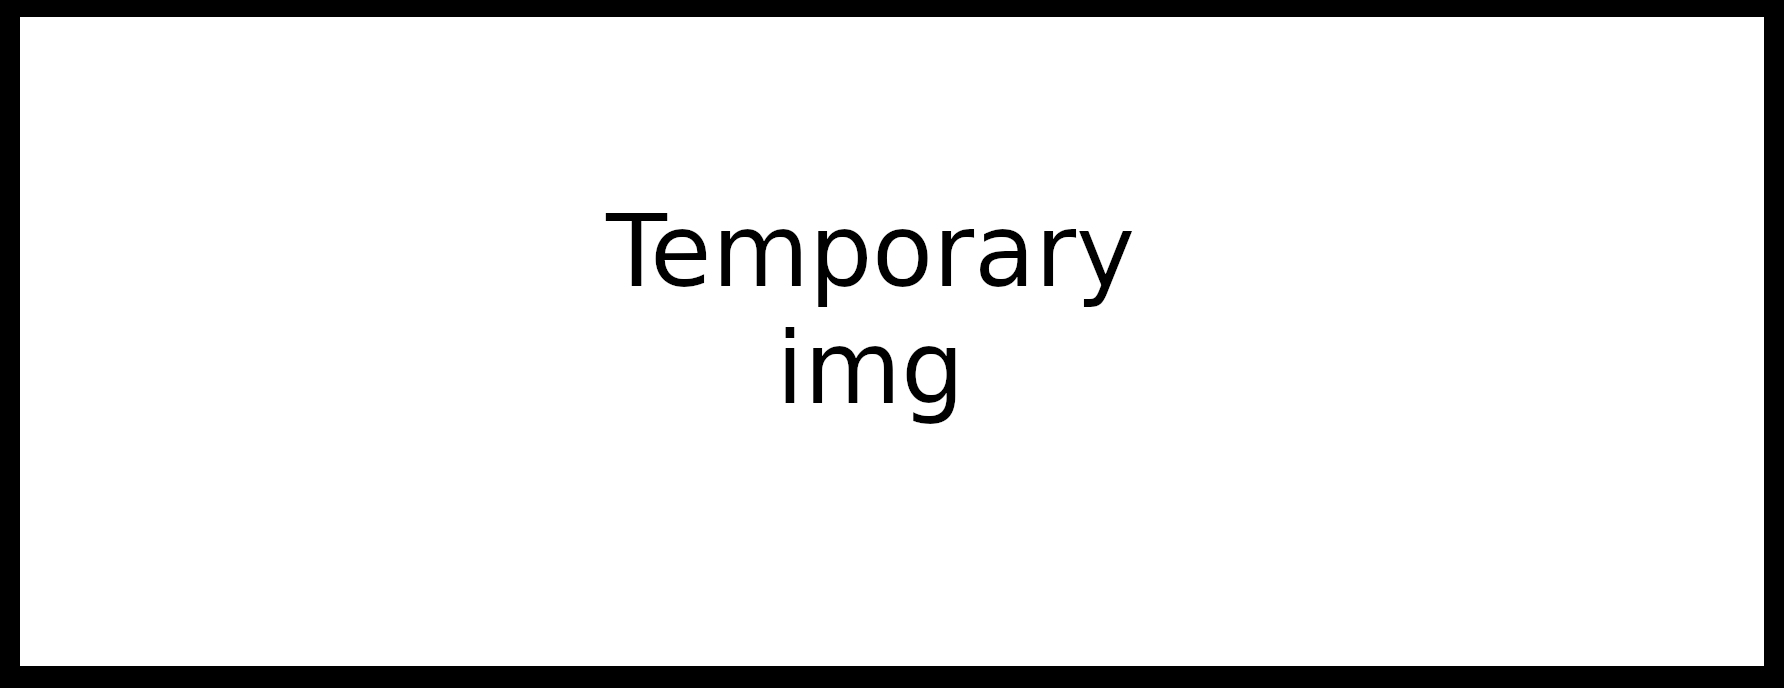
\includegraphics[width=0.3\textwidth]{resources/temp.png}
	\caption{A simple graphic}
	\label{fig:simple}	
\end{figure}


\subsubsection*{Non-numbered subsubsection}


\begin{description}
	\item [First] This is the first Item of a description list, could be useful if you need to name each procedure in a system, or in other ways list various components, while giving a short description of them.

	\item [Second] item in a list.
	

\end{description}

\lipsum[5]

\pagebreak

\todo{Remember that its easier to segment a paper into various sub-components, are you inserting large tables, tikz-pictures or other, then it might be wise to place them in a separeate tex and link it instead of having a gigantic single text file.}

\begin{figure}[htb]
	\centering
	\resizebox{\textwidth}{!}{\tikzset{
	data/.style={
		draw,
		rectangle split,
		rectangle split parts=2,
		text centered,
	},
	data+/.style={
		data,
		rectangle split every empty part={},% resets empty-part macro (explanation below)
		rectangle split empty part width=\widthof{#1},
		rectangle split empty part height=\heightof{#1},
		rectangle split empty part depth=\depthof{#1},
	},
}


\begin{tikzpicture}[background rectangle/.style={fill=green!15, rounded
	corners, draw=green!50}, show background rectangle, split/.style={rectangle split, rectangle split horizontal, rectangle split parts=#1, draw},splitv/.style={rectangle split, rectangle split parts=#1, draw}]



\node (R) {Root};
\node[split=1, above=0.25cm of R, fill=black!60] (A) {};


\node [data, right=1.0cm of A, fill=black!30] (B) { \nodepart{second} marked = True};
\draw[-stealth] ([yshift=0.5cm]A) -- (B);
\node [data, right=1.0cm of B, fill=black!30] (C) { \nodepart{second} marked = True};
\draw[-stealth, transform canvas={yshift=0.25cm}] (B) -- (C);
\node [data, right=1.0cm of C, fill=black!30] (D) { \nodepart{second} marked = True};
\draw[-stealth, transform canvas={yshift=0.25cm}] (C) -- (D);
\draw[-stealth, transform canvas={yshift=0.25cm}] (D) to[out=5, in=20] (B);

\node [data, below=1cm of B, fill=white] (B1) { \nodepart{second} marked = False};
\node [data, right=1.0cm of B1, fill=white] (C1) { \nodepart{second} marked = False};
\draw[-stealth, transform canvas={yshift=0.25cm}] (B1) -- (C1);
\node [data, right=1.0cm of C1, fill=black!30] (D1) { \nodepart{second} marked = True};
\draw[-stealth, transform canvas={yshift=0.25cm}] (C1) -- (D1);

\draw[-stealth, transform canvas={yshift=0.25cm}] (B1) to[out=20, in=-170,distance=0.5cm] (C);
\draw[-stealth, transform canvas={yshift=0.25cm}] (C) to[out=0, in=-190,distance=0.5cm] (D1);
\node[below=0.6cm of C1] {Illustration after a mark.};



\end{tikzpicture}}
	\caption{This image is a tex-document written in tikz.}
	\label{fig:tikz}
\end{figure}

\lipsum[2-4]

\pagebreak
\section{Method}
Variations on novelty search are often studied in the domain of maze navigation. Mazes are useful
since they allow for the construction of tasks of varying deceptiveness. If the objective function is
based on the distance to the end of the maze, simply following its gradient might trap the agent in
dead ends. The maze can be seen as an abstraction for difficult problems in which the fitness
landscape is deceptive.

\subsection{Maze navigation task}
In maze navigation, a simulated robot must solve a maze within a limited number of time steps.
The robot is controlled by a neural network which, given the readings from the robots sensors,
outputs two forces adjusting the robots linear and angular velocity.

The robot has six rangefinder sensors which measure the distance to walls. If a wall occurs within the sensors
direction and maximum range, the distance is returned. It also has four radar sensors which return binary
values indicating whether the end point is directly reachable within their field of view.

Three mazes are used to compare the novelty search variants (see Figure \ref{mazes}) similar to the ones in \cite{ns_study, novelty_alone}.
The first one is easy, only requiring the robot to slightly shift its path to reach the end point. The second is more
difficult, with deeper dead ends that require the robots to explore parts of the maze of much lower fitness.
The last maze is open at the top, the robots are free to move upwards from the actual maze.
$95 \%$ of the maze area is irrelevant to actually solving it. This creates a
large behaviour space which decouples novelty from utility, making novelty search alone insufficient
to solve it.

Any robot which navigates within 5 units of the end point is classified as having solved the maze. The robots
were given $400$ time steps to solve the maze, a limit which was set as to force them to navigate the maze
in a direct manner.


\begin{figure}[H]
    \captionsetup[subfigure]{justification=centering}
    \centering
    \begin{mdframed}
        \begin{subfigure}[b]{0.3\textwidth}
            \centering
            \scalebox{0.25}{%% Creator: Matplotlib, PGF backend
%%
%% To include the figure in your LaTeX document, write
%%   \input{<filename>.pgf}
%%
%% Make sure the required packages are loaded in your preamble
%%   \usepackage{pgf}
%%
%% and, on pdftex
%%   \usepackage[utf8]{inputenc}\DeclareUnicodeCharacter{2212}{-}
%%
%% or, on luatex and xetex
%%   \usepackage{unicode-math}
%%
%% Figures using additional raster images can only be included by \input if
%% they are in the same directory as the main LaTeX file. For loading figures
%% from other directories you can use the `import` package
%%   \usepackage{import}
%%
%% and then include the figures with
%%   \import{<path to file>}{<filename>.pgf}
%%
%% Matplotlib used the following preamble
%%
\begingroup%
\makeatletter%
\begin{pgfpicture}%
\pgfpathrectangle{\pgfpointorigin}{\pgfqpoint{6.400000in}{3.280000in}}%
\pgfusepath{use as bounding box, clip}%
\begin{pgfscope}%
\pgfsetbuttcap%
\pgfsetmiterjoin%
\definecolor{currentfill}{rgb}{1.000000,1.000000,1.000000}%
\pgfsetfillcolor{currentfill}%
\pgfsetlinewidth{0.000000pt}%
\definecolor{currentstroke}{rgb}{1.000000,1.000000,1.000000}%
\pgfsetstrokecolor{currentstroke}%
\pgfsetdash{}{0pt}%
\pgfpathmoveto{\pgfqpoint{0.000000in}{0.000000in}}%
\pgfpathlineto{\pgfqpoint{6.400000in}{0.000000in}}%
\pgfpathlineto{\pgfqpoint{6.400000in}{3.280000in}}%
\pgfpathlineto{\pgfqpoint{0.000000in}{3.280000in}}%
\pgfpathclose%
\pgfusepath{fill}%
\end{pgfscope}%
\begin{pgfscope}%
\pgfpathrectangle{\pgfqpoint{0.100000in}{0.100000in}}{\pgfqpoint{6.200000in}{3.080000in}}%
\pgfusepath{clip}%
\pgfsetbuttcap%
\pgfsetmiterjoin%
\definecolor{currentfill}{rgb}{0.600000,1.000000,0.600000}%
\pgfsetfillcolor{currentfill}%
\pgfsetlinewidth{1.003750pt}%
\definecolor{currentstroke}{rgb}{1.000000,1.000000,1.000000}%
\pgfsetstrokecolor{currentstroke}%
\pgfsetdash{}{0pt}%
\pgfpathmoveto{\pgfqpoint{0.565000in}{0.323300in}}%
\pgfpathcurveto{\pgfqpoint{0.595830in}{0.323300in}}{\pgfqpoint{0.625401in}{0.335470in}}{\pgfqpoint{0.647201in}{0.357129in}}%
\pgfpathcurveto{\pgfqpoint{0.669001in}{0.378789in}}{\pgfqpoint{0.681250in}{0.408169in}}{\pgfqpoint{0.681250in}{0.438800in}}%
\pgfpathcurveto{\pgfqpoint{0.681250in}{0.469431in}}{\pgfqpoint{0.669001in}{0.498811in}}{\pgfqpoint{0.647201in}{0.520471in}}%
\pgfpathcurveto{\pgfqpoint{0.625401in}{0.542130in}}{\pgfqpoint{0.595830in}{0.554300in}}{\pgfqpoint{0.565000in}{0.554300in}}%
\pgfpathcurveto{\pgfqpoint{0.534170in}{0.554300in}}{\pgfqpoint{0.504599in}{0.542130in}}{\pgfqpoint{0.482799in}{0.520471in}}%
\pgfpathcurveto{\pgfqpoint{0.460999in}{0.498811in}}{\pgfqpoint{0.448750in}{0.469431in}}{\pgfqpoint{0.448750in}{0.438800in}}%
\pgfpathcurveto{\pgfqpoint{0.448750in}{0.408169in}}{\pgfqpoint{0.460999in}{0.378789in}}{\pgfqpoint{0.482799in}{0.357129in}}%
\pgfpathcurveto{\pgfqpoint{0.504599in}{0.335470in}}{\pgfqpoint{0.534170in}{0.323300in}}{\pgfqpoint{0.565000in}{0.323300in}}%
\pgfpathclose%
\pgfusepath{stroke,fill}%
\end{pgfscope}%
\begin{pgfscope}%
\pgfpathrectangle{\pgfqpoint{0.100000in}{0.100000in}}{\pgfqpoint{6.200000in}{3.080000in}}%
\pgfusepath{clip}%
\pgfsetbuttcap%
\pgfsetmiterjoin%
\definecolor{currentfill}{rgb}{1.000000,0.200000,0.000000}%
\pgfsetfillcolor{currentfill}%
\pgfsetlinewidth{1.003750pt}%
\definecolor{currentstroke}{rgb}{1.000000,1.000000,1.000000}%
\pgfsetstrokecolor{currentstroke}%
\pgfsetdash{}{0pt}%
\pgfpathmoveto{\pgfqpoint{4.285000in}{1.524500in}}%
\pgfpathcurveto{\pgfqpoint{4.315830in}{1.524500in}}{\pgfqpoint{4.345401in}{1.536670in}}{\pgfqpoint{4.367201in}{1.558329in}}%
\pgfpathcurveto{\pgfqpoint{4.389001in}{1.579989in}}{\pgfqpoint{4.401250in}{1.609369in}}{\pgfqpoint{4.401250in}{1.640000in}}%
\pgfpathcurveto{\pgfqpoint{4.401250in}{1.670631in}}{\pgfqpoint{4.389001in}{1.700011in}}{\pgfqpoint{4.367201in}{1.721671in}}%
\pgfpathcurveto{\pgfqpoint{4.345401in}{1.743330in}}{\pgfqpoint{4.315830in}{1.755500in}}{\pgfqpoint{4.285000in}{1.755500in}}%
\pgfpathcurveto{\pgfqpoint{4.254170in}{1.755500in}}{\pgfqpoint{4.224599in}{1.743330in}}{\pgfqpoint{4.202799in}{1.721671in}}%
\pgfpathcurveto{\pgfqpoint{4.180999in}{1.700011in}}{\pgfqpoint{4.168750in}{1.670631in}}{\pgfqpoint{4.168750in}{1.640000in}}%
\pgfpathcurveto{\pgfqpoint{4.168750in}{1.609369in}}{\pgfqpoint{4.180999in}{1.579989in}}{\pgfqpoint{4.202799in}{1.558329in}}%
\pgfpathcurveto{\pgfqpoint{4.224599in}{1.536670in}}{\pgfqpoint{4.254170in}{1.524500in}}{\pgfqpoint{4.285000in}{1.524500in}}%
\pgfpathclose%
\pgfusepath{stroke,fill}%
\end{pgfscope}%
\begin{pgfscope}%
\pgfpathrectangle{\pgfqpoint{0.100000in}{0.100000in}}{\pgfqpoint{6.200000in}{3.080000in}}%
\pgfusepath{clip}%
\pgfsetrectcap%
\pgfsetroundjoin%
\pgfsetlinewidth{1.505625pt}%
\definecolor{currentstroke}{rgb}{0.121569,0.466667,0.705882}%
\pgfsetstrokecolor{currentstroke}%
\pgfsetdash{}{0pt}%
\pgfpathmoveto{\pgfqpoint{0.177500in}{0.177000in}}%
\pgfpathlineto{\pgfqpoint{4.672500in}{0.177000in}}%
\pgfusepath{stroke}%
\end{pgfscope}%
\begin{pgfscope}%
\pgfpathrectangle{\pgfqpoint{0.100000in}{0.100000in}}{\pgfqpoint{6.200000in}{3.080000in}}%
\pgfusepath{clip}%
\pgfsetrectcap%
\pgfsetroundjoin%
\pgfsetlinewidth{1.505625pt}%
\definecolor{currentstroke}{rgb}{0.121569,0.466667,0.705882}%
\pgfsetstrokecolor{currentstroke}%
\pgfsetdash{}{0pt}%
\pgfpathmoveto{\pgfqpoint{4.672500in}{0.177000in}}%
\pgfpathlineto{\pgfqpoint{4.672500in}{2.179000in}}%
\pgfusepath{stroke}%
\end{pgfscope}%
\begin{pgfscope}%
\pgfpathrectangle{\pgfqpoint{0.100000in}{0.100000in}}{\pgfqpoint{6.200000in}{3.080000in}}%
\pgfusepath{clip}%
\pgfsetrectcap%
\pgfsetroundjoin%
\pgfsetlinewidth{1.505625pt}%
\definecolor{currentstroke}{rgb}{0.121569,0.466667,0.705882}%
\pgfsetstrokecolor{currentstroke}%
\pgfsetdash{}{0pt}%
\pgfpathmoveto{\pgfqpoint{4.672500in}{2.179000in}}%
\pgfpathlineto{\pgfqpoint{0.177500in}{2.179000in}}%
\pgfusepath{stroke}%
\end{pgfscope}%
\begin{pgfscope}%
\pgfpathrectangle{\pgfqpoint{0.100000in}{0.100000in}}{\pgfqpoint{6.200000in}{3.080000in}}%
\pgfusepath{clip}%
\pgfsetrectcap%
\pgfsetroundjoin%
\pgfsetlinewidth{1.505625pt}%
\definecolor{currentstroke}{rgb}{0.121569,0.466667,0.705882}%
\pgfsetstrokecolor{currentstroke}%
\pgfsetdash{}{0pt}%
\pgfpathmoveto{\pgfqpoint{0.177500in}{2.179000in}}%
\pgfpathlineto{\pgfqpoint{0.177500in}{0.177000in}}%
\pgfusepath{stroke}%
\end{pgfscope}%
\begin{pgfscope}%
\pgfpathrectangle{\pgfqpoint{0.100000in}{0.100000in}}{\pgfqpoint{6.200000in}{3.080000in}}%
\pgfusepath{clip}%
\pgfsetrectcap%
\pgfsetroundjoin%
\pgfsetlinewidth{1.505625pt}%
\definecolor{currentstroke}{rgb}{0.121569,0.466667,0.705882}%
\pgfsetstrokecolor{currentstroke}%
\pgfsetdash{}{0pt}%
\pgfpathmoveto{\pgfqpoint{3.835500in}{2.179000in}}%
\pgfpathlineto{\pgfqpoint{0.999000in}{1.101000in}}%
\pgfusepath{stroke}%
\end{pgfscope}%
\begin{pgfscope}%
\pgfpathrectangle{\pgfqpoint{0.100000in}{0.100000in}}{\pgfqpoint{6.200000in}{3.080000in}}%
\pgfusepath{clip}%
\pgfsetrectcap%
\pgfsetroundjoin%
\pgfsetlinewidth{1.505625pt}%
\definecolor{currentstroke}{rgb}{0.121569,0.466667,0.705882}%
\pgfsetstrokecolor{currentstroke}%
\pgfsetdash{}{0pt}%
\pgfpathmoveto{\pgfqpoint{1.867000in}{0.177000in}}%
\pgfpathlineto{\pgfqpoint{1.231500in}{0.746800in}}%
\pgfusepath{stroke}%
\end{pgfscope}%
\begin{pgfscope}%
\pgfpathrectangle{\pgfqpoint{0.100000in}{0.100000in}}{\pgfqpoint{6.200000in}{3.080000in}}%
\pgfusepath{clip}%
\pgfsetrectcap%
\pgfsetroundjoin%
\pgfsetlinewidth{1.505625pt}%
\definecolor{currentstroke}{rgb}{0.121569,0.466667,0.705882}%
\pgfsetstrokecolor{currentstroke}%
\pgfsetdash{}{0pt}%
\pgfpathmoveto{\pgfqpoint{2.115000in}{1.501400in}}%
\pgfpathlineto{\pgfqpoint{1.758500in}{0.808400in}}%
\pgfusepath{stroke}%
\end{pgfscope}%
\begin{pgfscope}%
\pgfpathrectangle{\pgfqpoint{0.100000in}{0.100000in}}{\pgfqpoint{6.200000in}{3.080000in}}%
\pgfusepath{clip}%
\pgfsetrectcap%
\pgfsetroundjoin%
\pgfsetlinewidth{1.505625pt}%
\definecolor{currentstroke}{rgb}{0.121569,0.466667,0.705882}%
\pgfsetstrokecolor{currentstroke}%
\pgfsetdash{}{0pt}%
\pgfpathmoveto{\pgfqpoint{3.138000in}{0.177000in}}%
\pgfpathlineto{\pgfqpoint{2.254500in}{0.885400in}}%
\pgfusepath{stroke}%
\end{pgfscope}%
\begin{pgfscope}%
\pgfpathrectangle{\pgfqpoint{0.100000in}{0.100000in}}{\pgfqpoint{6.200000in}{3.080000in}}%
\pgfusepath{clip}%
\pgfsetrectcap%
\pgfsetroundjoin%
\pgfsetlinewidth{1.505625pt}%
\definecolor{currentstroke}{rgb}{0.121569,0.466667,0.705882}%
\pgfsetstrokecolor{currentstroke}%
\pgfsetdash{}{0pt}%
\pgfpathmoveto{\pgfqpoint{3.494500in}{2.025000in}}%
\pgfpathlineto{\pgfqpoint{2.921000in}{1.070200in}}%
\pgfusepath{stroke}%
\end{pgfscope}%
\begin{pgfscope}%
\pgfpathrectangle{\pgfqpoint{0.100000in}{0.100000in}}{\pgfqpoint{6.200000in}{3.080000in}}%
\pgfusepath{clip}%
\pgfsetrectcap%
\pgfsetroundjoin%
\pgfsetlinewidth{1.505625pt}%
\definecolor{currentstroke}{rgb}{0.121569,0.466667,0.705882}%
\pgfsetstrokecolor{currentstroke}%
\pgfsetdash{}{0pt}%
\pgfpathmoveto{\pgfqpoint{4.238500in}{0.177000in}}%
\pgfpathlineto{\pgfqpoint{3.417000in}{1.070200in}}%
\pgfusepath{stroke}%
\end{pgfscope}%
\begin{pgfscope}%
\pgfpathrectangle{\pgfqpoint{0.100000in}{0.100000in}}{\pgfqpoint{6.200000in}{3.080000in}}%
\pgfusepath{clip}%
\pgfsetrectcap%
\pgfsetroundjoin%
\pgfsetlinewidth{1.505625pt}%
\definecolor{currentstroke}{rgb}{0.121569,0.466667,0.705882}%
\pgfsetstrokecolor{currentstroke}%
\pgfsetdash{}{0pt}%
\pgfpathmoveto{\pgfqpoint{4.300500in}{2.179000in}}%
\pgfpathlineto{\pgfqpoint{3.773500in}{1.455200in}}%
\pgfusepath{stroke}%
\end{pgfscope}%
\end{pgfpicture}%
\makeatother%
\endgroup%
}
            \caption{Medium.}
        \end{subfigure}
        \begin{subfigure}[b]{0.3\textwidth}
            \centering
            \scalebox{0.25}{%% Creator: Matplotlib, PGF backend
%%
%% To include the figure in your LaTeX document, write
%%   \input{<filename>.pgf}
%%
%% Make sure the required packages are loaded in your preamble
%%   \usepackage{pgf}
%%
%% and, on pdftex
%%   \usepackage[utf8]{inputenc}\DeclareUnicodeCharacter{2212}{-}
%%
%% or, on luatex and xetex
%%   \usepackage{unicode-math}
%%
%% Figures using additional raster images can only be included by \input if
%% they are in the same directory as the main LaTeX file. For loading figures
%% from other directories you can use the `import` package
%%   \usepackage{import}
%%
%% and then include the figures with
%%   \import{<path to file>}{<filename>.pgf}
%%
%% Matplotlib used the following preamble
%%
\begingroup%
\makeatletter%
\begin{pgfpicture}%
\pgfpathrectangle{\pgfpointorigin}{\pgfqpoint{6.400000in}{3.280000in}}%
\pgfusepath{use as bounding box, clip}%
\begin{pgfscope}%
\pgfsetbuttcap%
\pgfsetmiterjoin%
\definecolor{currentfill}{rgb}{1.000000,1.000000,1.000000}%
\pgfsetfillcolor{currentfill}%
\pgfsetlinewidth{0.000000pt}%
\definecolor{currentstroke}{rgb}{1.000000,1.000000,1.000000}%
\pgfsetstrokecolor{currentstroke}%
\pgfsetdash{}{0pt}%
\pgfpathmoveto{\pgfqpoint{0.000000in}{0.000000in}}%
\pgfpathlineto{\pgfqpoint{6.400000in}{0.000000in}}%
\pgfpathlineto{\pgfqpoint{6.400000in}{3.280000in}}%
\pgfpathlineto{\pgfqpoint{0.000000in}{3.280000in}}%
\pgfpathclose%
\pgfusepath{fill}%
\end{pgfscope}%
\begin{pgfscope}%
\pgfpathrectangle{\pgfqpoint{0.100000in}{0.100000in}}{\pgfqpoint{6.200000in}{3.080000in}}%
\pgfusepath{clip}%
\pgfsetbuttcap%
\pgfsetmiterjoin%
\definecolor{currentfill}{rgb}{0.600000,1.000000,0.600000}%
\pgfsetfillcolor{currentfill}%
\pgfsetlinewidth{1.003750pt}%
\definecolor{currentstroke}{rgb}{1.000000,1.000000,1.000000}%
\pgfsetstrokecolor{currentstroke}%
\pgfsetdash{}{0pt}%
\pgfpathmoveto{\pgfqpoint{0.658000in}{2.818100in}}%
\pgfpathcurveto{\pgfqpoint{0.688830in}{2.818100in}}{\pgfqpoint{0.718401in}{2.830270in}}{\pgfqpoint{0.740201in}{2.851929in}}%
\pgfpathcurveto{\pgfqpoint{0.762001in}{2.873589in}}{\pgfqpoint{0.774250in}{2.902969in}}{\pgfqpoint{0.774250in}{2.933600in}}%
\pgfpathcurveto{\pgfqpoint{0.774250in}{2.964231in}}{\pgfqpoint{0.762001in}{2.993611in}}{\pgfqpoint{0.740201in}{3.015271in}}%
\pgfpathcurveto{\pgfqpoint{0.718401in}{3.036930in}}{\pgfqpoint{0.688830in}{3.049100in}}{\pgfqpoint{0.658000in}{3.049100in}}%
\pgfpathcurveto{\pgfqpoint{0.627170in}{3.049100in}}{\pgfqpoint{0.597599in}{3.036930in}}{\pgfqpoint{0.575799in}{3.015271in}}%
\pgfpathcurveto{\pgfqpoint{0.553999in}{2.993611in}}{\pgfqpoint{0.541750in}{2.964231in}}{\pgfqpoint{0.541750in}{2.933600in}}%
\pgfpathcurveto{\pgfqpoint{0.541750in}{2.902969in}}{\pgfqpoint{0.553999in}{2.873589in}}{\pgfqpoint{0.575799in}{2.851929in}}%
\pgfpathcurveto{\pgfqpoint{0.597599in}{2.830270in}}{\pgfqpoint{0.627170in}{2.818100in}}{\pgfqpoint{0.658000in}{2.818100in}}%
\pgfpathclose%
\pgfusepath{stroke,fill}%
\end{pgfscope}%
\begin{pgfscope}%
\pgfpathrectangle{\pgfqpoint{0.100000in}{0.100000in}}{\pgfqpoint{6.200000in}{3.080000in}}%
\pgfusepath{clip}%
\pgfsetbuttcap%
\pgfsetmiterjoin%
\definecolor{currentfill}{rgb}{1.000000,0.200000,0.000000}%
\pgfsetfillcolor{currentfill}%
\pgfsetlinewidth{1.003750pt}%
\definecolor{currentstroke}{rgb}{1.000000,1.000000,1.000000}%
\pgfsetstrokecolor{currentstroke}%
\pgfsetdash{}{0pt}%
\pgfpathmoveto{\pgfqpoint{0.580500in}{0.292500in}}%
\pgfpathcurveto{\pgfqpoint{0.611330in}{0.292500in}}{\pgfqpoint{0.640901in}{0.304670in}}{\pgfqpoint{0.662701in}{0.326329in}}%
\pgfpathcurveto{\pgfqpoint{0.684501in}{0.347989in}}{\pgfqpoint{0.696750in}{0.377369in}}{\pgfqpoint{0.696750in}{0.408000in}}%
\pgfpathcurveto{\pgfqpoint{0.696750in}{0.438631in}}{\pgfqpoint{0.684501in}{0.468011in}}{\pgfqpoint{0.662701in}{0.489671in}}%
\pgfpathcurveto{\pgfqpoint{0.640901in}{0.511330in}}{\pgfqpoint{0.611330in}{0.523500in}}{\pgfqpoint{0.580500in}{0.523500in}}%
\pgfpathcurveto{\pgfqpoint{0.549670in}{0.523500in}}{\pgfqpoint{0.520099in}{0.511330in}}{\pgfqpoint{0.498299in}{0.489671in}}%
\pgfpathcurveto{\pgfqpoint{0.476499in}{0.468011in}}{\pgfqpoint{0.464250in}{0.438631in}}{\pgfqpoint{0.464250in}{0.408000in}}%
\pgfpathcurveto{\pgfqpoint{0.464250in}{0.377369in}}{\pgfqpoint{0.476499in}{0.347989in}}{\pgfqpoint{0.498299in}{0.326329in}}%
\pgfpathcurveto{\pgfqpoint{0.520099in}{0.304670in}}{\pgfqpoint{0.549670in}{0.292500in}}{\pgfqpoint{0.580500in}{0.292500in}}%
\pgfpathclose%
\pgfusepath{stroke,fill}%
\end{pgfscope}%
\begin{pgfscope}%
\pgfpathrectangle{\pgfqpoint{0.100000in}{0.100000in}}{\pgfqpoint{6.200000in}{3.080000in}}%
\pgfusepath{clip}%
\pgfsetrectcap%
\pgfsetroundjoin%
\pgfsetlinewidth{1.505625pt}%
\definecolor{currentstroke}{rgb}{0.121569,0.466667,0.705882}%
\pgfsetstrokecolor{currentstroke}%
\pgfsetdash{}{0pt}%
\pgfpathmoveto{\pgfqpoint{0.177500in}{0.177000in}}%
\pgfpathlineto{\pgfqpoint{0.177500in}{3.180000in}}%
\pgfusepath{stroke}%
\end{pgfscope}%
\begin{pgfscope}%
\pgfpathrectangle{\pgfqpoint{0.100000in}{0.100000in}}{\pgfqpoint{6.200000in}{3.080000in}}%
\pgfusepath{clip}%
\pgfsetrectcap%
\pgfsetroundjoin%
\pgfsetlinewidth{1.505625pt}%
\definecolor{currentstroke}{rgb}{0.121569,0.466667,0.705882}%
\pgfsetstrokecolor{currentstroke}%
\pgfsetdash{}{0pt}%
\pgfpathmoveto{\pgfqpoint{0.177500in}{3.180000in}}%
\pgfpathlineto{\pgfqpoint{3.200000in}{3.180000in}}%
\pgfusepath{stroke}%
\end{pgfscope}%
\begin{pgfscope}%
\pgfpathrectangle{\pgfqpoint{0.100000in}{0.100000in}}{\pgfqpoint{6.200000in}{3.080000in}}%
\pgfusepath{clip}%
\pgfsetrectcap%
\pgfsetroundjoin%
\pgfsetlinewidth{1.505625pt}%
\definecolor{currentstroke}{rgb}{0.121569,0.466667,0.705882}%
\pgfsetstrokecolor{currentstroke}%
\pgfsetdash{}{0pt}%
\pgfpathmoveto{\pgfqpoint{3.200000in}{3.180000in}}%
\pgfpathlineto{\pgfqpoint{3.200000in}{0.177000in}}%
\pgfusepath{stroke}%
\end{pgfscope}%
\begin{pgfscope}%
\pgfpathrectangle{\pgfqpoint{0.100000in}{0.100000in}}{\pgfqpoint{6.200000in}{3.080000in}}%
\pgfusepath{clip}%
\pgfsetrectcap%
\pgfsetroundjoin%
\pgfsetlinewidth{1.505625pt}%
\definecolor{currentstroke}{rgb}{0.121569,0.466667,0.705882}%
\pgfsetstrokecolor{currentstroke}%
\pgfsetdash{}{0pt}%
\pgfpathmoveto{\pgfqpoint{3.200000in}{0.177000in}}%
\pgfpathlineto{\pgfqpoint{0.177500in}{0.177000in}}%
\pgfusepath{stroke}%
\end{pgfscope}%
\begin{pgfscope}%
\pgfpathrectangle{\pgfqpoint{0.100000in}{0.100000in}}{\pgfqpoint{6.200000in}{3.080000in}}%
\pgfusepath{clip}%
\pgfsetrectcap%
\pgfsetroundjoin%
\pgfsetlinewidth{1.505625pt}%
\definecolor{currentstroke}{rgb}{0.121569,0.466667,0.705882}%
\pgfsetstrokecolor{currentstroke}%
\pgfsetdash{}{0pt}%
\pgfpathmoveto{\pgfqpoint{0.177500in}{0.854600in}}%
\pgfpathlineto{\pgfqpoint{0.983500in}{0.916200in}}%
\pgfusepath{stroke}%
\end{pgfscope}%
\begin{pgfscope}%
\pgfpathrectangle{\pgfqpoint{0.100000in}{0.100000in}}{\pgfqpoint{6.200000in}{3.080000in}}%
\pgfusepath{clip}%
\pgfsetrectcap%
\pgfsetroundjoin%
\pgfsetlinewidth{1.505625pt}%
\definecolor{currentstroke}{rgb}{0.121569,0.466667,0.705882}%
\pgfsetstrokecolor{currentstroke}%
\pgfsetdash{}{0pt}%
\pgfpathmoveto{\pgfqpoint{0.968000in}{0.931600in}}%
\pgfpathlineto{\pgfqpoint{0.968000in}{2.517800in}}%
\pgfusepath{stroke}%
\end{pgfscope}%
\begin{pgfscope}%
\pgfpathrectangle{\pgfqpoint{0.100000in}{0.100000in}}{\pgfqpoint{6.200000in}{3.080000in}}%
\pgfusepath{clip}%
\pgfsetrectcap%
\pgfsetroundjoin%
\pgfsetlinewidth{1.505625pt}%
\definecolor{currentstroke}{rgb}{0.121569,0.466667,0.705882}%
\pgfsetstrokecolor{currentstroke}%
\pgfsetdash{}{0pt}%
\pgfpathmoveto{\pgfqpoint{0.983500in}{1.732400in}}%
\pgfpathlineto{\pgfqpoint{2.549000in}{2.594800in}}%
\pgfusepath{stroke}%
\end{pgfscope}%
\begin{pgfscope}%
\pgfpathrectangle{\pgfqpoint{0.100000in}{0.100000in}}{\pgfqpoint{6.200000in}{3.080000in}}%
\pgfusepath{clip}%
\pgfsetrectcap%
\pgfsetroundjoin%
\pgfsetlinewidth{1.505625pt}%
\definecolor{currentstroke}{rgb}{0.121569,0.466667,0.705882}%
\pgfsetstrokecolor{currentstroke}%
\pgfsetdash{}{0pt}%
\pgfpathmoveto{\pgfqpoint{1.293500in}{3.180000in}}%
\pgfpathlineto{\pgfqpoint{1.774000in}{2.625600in}}%
\pgfusepath{stroke}%
\end{pgfscope}%
\begin{pgfscope}%
\pgfpathrectangle{\pgfqpoint{0.100000in}{0.100000in}}{\pgfqpoint{6.200000in}{3.080000in}}%
\pgfusepath{clip}%
\pgfsetrectcap%
\pgfsetroundjoin%
\pgfsetlinewidth{1.505625pt}%
\definecolor{currentstroke}{rgb}{0.121569,0.466667,0.705882}%
\pgfsetstrokecolor{currentstroke}%
\pgfsetdash{}{0pt}%
\pgfpathmoveto{\pgfqpoint{0.177500in}{1.332000in}}%
\pgfpathlineto{\pgfqpoint{0.611500in}{1.963400in}}%
\pgfusepath{stroke}%
\end{pgfscope}%
\begin{pgfscope}%
\pgfpathrectangle{\pgfqpoint{0.100000in}{0.100000in}}{\pgfqpoint{6.200000in}{3.080000in}}%
\pgfusepath{clip}%
\pgfsetrectcap%
\pgfsetroundjoin%
\pgfsetlinewidth{1.505625pt}%
\definecolor{currentstroke}{rgb}{0.121569,0.466667,0.705882}%
\pgfsetstrokecolor{currentstroke}%
\pgfsetdash{}{0pt}%
\pgfpathmoveto{\pgfqpoint{3.200000in}{2.348400in}}%
\pgfpathlineto{\pgfqpoint{1.448500in}{1.501400in}}%
\pgfusepath{stroke}%
\end{pgfscope}%
\begin{pgfscope}%
\pgfpathrectangle{\pgfqpoint{0.100000in}{0.100000in}}{\pgfqpoint{6.200000in}{3.080000in}}%
\pgfusepath{clip}%
\pgfsetrectcap%
\pgfsetroundjoin%
\pgfsetlinewidth{1.505625pt}%
\definecolor{currentstroke}{rgb}{0.121569,0.466667,0.705882}%
\pgfsetstrokecolor{currentstroke}%
\pgfsetdash{}{0pt}%
\pgfpathmoveto{\pgfqpoint{0.968000in}{0.947000in}}%
\pgfpathlineto{\pgfqpoint{2.161500in}{0.562000in}}%
\pgfusepath{stroke}%
\end{pgfscope}%
\end{pgfpicture}%
\makeatother%
\endgroup%
}
            \caption{Hard.}
        \end{subfigure}
        \begin{subfigure}[b]{0.3\textwidth}
            \centering
            \scalebox{0.25}{%% Creator: Matplotlib, PGF backend
%%
%% To include the figure in your LaTeX document, write
%%   \input{<filename>.pgf}
%%
%% Make sure the required packages are loaded in your preamble
%%   \usepackage{pgf}
%%
%% and, on pdftex
%%   \usepackage[utf8]{inputenc}\DeclareUnicodeCharacter{2212}{-}
%%
%% or, on luatex and xetex
%%   \usepackage{unicode-math}
%%
%% Figures using additional raster images can only be included by \input if
%% they are in the same directory as the main LaTeX file. For loading figures
%% from other directories you can use the `import` package
%%   \usepackage{import}
%%
%% and then include the figures with
%%   \import{<path to file>}{<filename>.pgf}
%%
%% Matplotlib used the following preamble
%%
\begingroup%
\makeatletter%
\begin{pgfpicture}%
\pgfpathrectangle{\pgfpointorigin}{\pgfqpoint{5.160000in}{3.896000in}}%
\pgfusepath{use as bounding box, clip}%
\begin{pgfscope}%
\pgfsetbuttcap%
\pgfsetmiterjoin%
\definecolor{currentfill}{rgb}{1.000000,1.000000,1.000000}%
\pgfsetfillcolor{currentfill}%
\pgfsetlinewidth{0.000000pt}%
\definecolor{currentstroke}{rgb}{1.000000,1.000000,1.000000}%
\pgfsetstrokecolor{currentstroke}%
\pgfsetdash{}{0pt}%
\pgfpathmoveto{\pgfqpoint{0.000000in}{0.000000in}}%
\pgfpathlineto{\pgfqpoint{5.160000in}{0.000000in}}%
\pgfpathlineto{\pgfqpoint{5.160000in}{3.896000in}}%
\pgfpathlineto{\pgfqpoint{0.000000in}{3.896000in}}%
\pgfpathclose%
\pgfusepath{fill}%
\end{pgfscope}%
\begin{pgfscope}%
\pgfpathrectangle{\pgfqpoint{0.100000in}{0.100000in}}{\pgfqpoint{4.960000in}{3.696000in}}%
\pgfusepath{clip}%
\pgfsetbuttcap%
\pgfsetmiterjoin%
\definecolor{currentfill}{rgb}{0.000000,0.501961,0.000000}%
\pgfsetfillcolor{currentfill}%
\pgfsetlinewidth{0.000000pt}%
\definecolor{currentstroke}{rgb}{0.000000,0.000000,0.000000}%
\pgfsetstrokecolor{currentstroke}%
\pgfsetstrokeopacity{0.000000}%
\pgfsetdash{}{0pt}%
\pgfpathmoveto{\pgfqpoint{0.992800in}{3.407920in}}%
\pgfpathcurveto{\pgfqpoint{1.025685in}{3.407920in}}{\pgfqpoint{1.057228in}{3.417656in}}{\pgfqpoint{1.080481in}{3.434983in}}%
\pgfpathcurveto{\pgfqpoint{1.103735in}{3.452311in}}{\pgfqpoint{1.116800in}{3.475815in}}{\pgfqpoint{1.116800in}{3.500320in}}%
\pgfpathcurveto{\pgfqpoint{1.116800in}{3.524825in}}{\pgfqpoint{1.103735in}{3.548329in}}{\pgfqpoint{1.080481in}{3.565657in}}%
\pgfpathcurveto{\pgfqpoint{1.057228in}{3.582984in}}{\pgfqpoint{1.025685in}{3.592720in}}{\pgfqpoint{0.992800in}{3.592720in}}%
\pgfpathcurveto{\pgfqpoint{0.959915in}{3.592720in}}{\pgfqpoint{0.928372in}{3.582984in}}{\pgfqpoint{0.905119in}{3.565657in}}%
\pgfpathcurveto{\pgfqpoint{0.881865in}{3.548329in}}{\pgfqpoint{0.868800in}{3.524825in}}{\pgfqpoint{0.868800in}{3.500320in}}%
\pgfpathcurveto{\pgfqpoint{0.868800in}{3.475815in}}{\pgfqpoint{0.881865in}{3.452311in}}{\pgfqpoint{0.905119in}{3.434983in}}%
\pgfpathcurveto{\pgfqpoint{0.928372in}{3.417656in}}{\pgfqpoint{0.959915in}{3.407920in}}{\pgfqpoint{0.992800in}{3.407920in}}%
\pgfpathclose%
\pgfusepath{fill}%
\end{pgfscope}%
\begin{pgfscope}%
\pgfpathrectangle{\pgfqpoint{0.100000in}{0.100000in}}{\pgfqpoint{4.960000in}{3.696000in}}%
\pgfusepath{clip}%
\pgfsetbuttcap%
\pgfsetmiterjoin%
\definecolor{currentfill}{rgb}{1.000000,0.000000,0.000000}%
\pgfsetfillcolor{currentfill}%
\pgfsetlinewidth{0.000000pt}%
\definecolor{currentstroke}{rgb}{0.000000,0.000000,0.000000}%
\pgfsetstrokecolor{currentstroke}%
\pgfsetstrokeopacity{0.000000}%
\pgfsetdash{}{0pt}%
\pgfpathmoveto{\pgfqpoint{0.868800in}{0.377200in}}%
\pgfpathcurveto{\pgfqpoint{0.901685in}{0.377200in}}{\pgfqpoint{0.933228in}{0.386936in}}{\pgfqpoint{0.956481in}{0.404263in}}%
\pgfpathcurveto{\pgfqpoint{0.979735in}{0.421591in}}{\pgfqpoint{0.992800in}{0.445095in}}{\pgfqpoint{0.992800in}{0.469600in}}%
\pgfpathcurveto{\pgfqpoint{0.992800in}{0.494105in}}{\pgfqpoint{0.979735in}{0.517609in}}{\pgfqpoint{0.956481in}{0.534937in}}%
\pgfpathcurveto{\pgfqpoint{0.933228in}{0.552264in}}{\pgfqpoint{0.901685in}{0.562000in}}{\pgfqpoint{0.868800in}{0.562000in}}%
\pgfpathcurveto{\pgfqpoint{0.835915in}{0.562000in}}{\pgfqpoint{0.804372in}{0.552264in}}{\pgfqpoint{0.781119in}{0.534937in}}%
\pgfpathcurveto{\pgfqpoint{0.757865in}{0.517609in}}{\pgfqpoint{0.744800in}{0.494105in}}{\pgfqpoint{0.744800in}{0.469600in}}%
\pgfpathcurveto{\pgfqpoint{0.744800in}{0.445095in}}{\pgfqpoint{0.757865in}{0.421591in}}{\pgfqpoint{0.781119in}{0.404263in}}%
\pgfpathcurveto{\pgfqpoint{0.804372in}{0.386936in}}{\pgfqpoint{0.835915in}{0.377200in}}{\pgfqpoint{0.868800in}{0.377200in}}%
\pgfpathclose%
\pgfusepath{fill}%
\end{pgfscope}%
\begin{pgfscope}%
\pgfpathrectangle{\pgfqpoint{0.100000in}{0.100000in}}{\pgfqpoint{4.960000in}{3.696000in}}%
\pgfusepath{clip}%
\pgfsetrectcap%
\pgfsetroundjoin%
\pgfsetlinewidth{1.505625pt}%
\definecolor{currentstroke}{rgb}{0.121569,0.466667,0.705882}%
\pgfsetstrokecolor{currentstroke}%
\pgfsetdash{}{0pt}%
\pgfpathmoveto{\pgfqpoint{0.224000in}{0.192400in}}%
\pgfpathlineto{\pgfqpoint{0.224000in}{3.806000in}}%
\pgfusepath{stroke}%
\end{pgfscope}%
\begin{pgfscope}%
\pgfpathrectangle{\pgfqpoint{0.100000in}{0.100000in}}{\pgfqpoint{4.960000in}{3.696000in}}%
\pgfusepath{clip}%
\pgfsetrectcap%
\pgfsetroundjoin%
\pgfsetlinewidth{1.505625pt}%
\definecolor{currentstroke}{rgb}{0.121569,0.466667,0.705882}%
\pgfsetstrokecolor{currentstroke}%
\pgfsetdash{}{0pt}%
\pgfusepath{stroke}%
\end{pgfscope}%
\begin{pgfscope}%
\pgfpathrectangle{\pgfqpoint{0.100000in}{0.100000in}}{\pgfqpoint{4.960000in}{3.696000in}}%
\pgfusepath{clip}%
\pgfsetrectcap%
\pgfsetroundjoin%
\pgfsetlinewidth{1.505625pt}%
\definecolor{currentstroke}{rgb}{0.121569,0.466667,0.705882}%
\pgfsetstrokecolor{currentstroke}%
\pgfsetdash{}{0pt}%
\pgfpathmoveto{\pgfqpoint{5.060000in}{3.806000in}}%
\pgfpathlineto{\pgfqpoint{5.060000in}{0.192400in}}%
\pgfusepath{stroke}%
\end{pgfscope}%
\begin{pgfscope}%
\pgfpathrectangle{\pgfqpoint{0.100000in}{0.100000in}}{\pgfqpoint{4.960000in}{3.696000in}}%
\pgfusepath{clip}%
\pgfsetrectcap%
\pgfsetroundjoin%
\pgfsetlinewidth{1.505625pt}%
\definecolor{currentstroke}{rgb}{0.121569,0.466667,0.705882}%
\pgfsetstrokecolor{currentstroke}%
\pgfsetdash{}{0pt}%
\pgfpathmoveto{\pgfqpoint{5.060000in}{0.192400in}}%
\pgfpathlineto{\pgfqpoint{0.224000in}{0.192400in}}%
\pgfusepath{stroke}%
\end{pgfscope}%
\begin{pgfscope}%
\pgfpathrectangle{\pgfqpoint{0.100000in}{0.100000in}}{\pgfqpoint{4.960000in}{3.696000in}}%
\pgfusepath{clip}%
\pgfsetrectcap%
\pgfsetroundjoin%
\pgfsetlinewidth{1.505625pt}%
\definecolor{currentstroke}{rgb}{0.121569,0.466667,0.705882}%
\pgfsetstrokecolor{currentstroke}%
\pgfsetdash{}{0pt}%
\pgfpathmoveto{\pgfqpoint{0.224000in}{1.005520in}}%
\pgfpathlineto{\pgfqpoint{1.513600in}{1.079440in}}%
\pgfusepath{stroke}%
\end{pgfscope}%
\begin{pgfscope}%
\pgfpathrectangle{\pgfqpoint{0.100000in}{0.100000in}}{\pgfqpoint{4.960000in}{3.696000in}}%
\pgfusepath{clip}%
\pgfsetrectcap%
\pgfsetroundjoin%
\pgfsetlinewidth{1.505625pt}%
\definecolor{currentstroke}{rgb}{0.121569,0.466667,0.705882}%
\pgfsetstrokecolor{currentstroke}%
\pgfsetdash{}{0pt}%
\pgfpathmoveto{\pgfqpoint{1.488800in}{1.097920in}}%
\pgfpathlineto{\pgfqpoint{1.488800in}{3.001360in}}%
\pgfusepath{stroke}%
\end{pgfscope}%
\begin{pgfscope}%
\pgfpathrectangle{\pgfqpoint{0.100000in}{0.100000in}}{\pgfqpoint{4.960000in}{3.696000in}}%
\pgfusepath{clip}%
\pgfsetrectcap%
\pgfsetroundjoin%
\pgfsetlinewidth{1.505625pt}%
\definecolor{currentstroke}{rgb}{0.121569,0.466667,0.705882}%
\pgfsetstrokecolor{currentstroke}%
\pgfsetdash{}{0pt}%
\pgfpathmoveto{\pgfqpoint{1.513600in}{2.058880in}}%
\pgfpathlineto{\pgfqpoint{4.018400in}{3.093760in}}%
\pgfusepath{stroke}%
\end{pgfscope}%
\begin{pgfscope}%
\pgfpathrectangle{\pgfqpoint{0.100000in}{0.100000in}}{\pgfqpoint{4.960000in}{3.696000in}}%
\pgfusepath{clip}%
\pgfsetrectcap%
\pgfsetroundjoin%
\pgfsetlinewidth{1.505625pt}%
\definecolor{currentstroke}{rgb}{0.121569,0.466667,0.705882}%
\pgfsetstrokecolor{currentstroke}%
\pgfsetdash{}{0pt}%
\pgfpathmoveto{\pgfqpoint{0.224000in}{1.578400in}}%
\pgfpathlineto{\pgfqpoint{0.918400in}{2.336080in}}%
\pgfusepath{stroke}%
\end{pgfscope}%
\begin{pgfscope}%
\pgfpathrectangle{\pgfqpoint{0.100000in}{0.100000in}}{\pgfqpoint{4.960000in}{3.696000in}}%
\pgfusepath{clip}%
\pgfsetrectcap%
\pgfsetroundjoin%
\pgfsetlinewidth{1.505625pt}%
\definecolor{currentstroke}{rgb}{0.121569,0.466667,0.705882}%
\pgfsetstrokecolor{currentstroke}%
\pgfsetdash{}{0pt}%
\pgfpathmoveto{\pgfqpoint{5.060000in}{2.798080in}}%
\pgfpathlineto{\pgfqpoint{2.257600in}{1.781680in}}%
\pgfusepath{stroke}%
\end{pgfscope}%
\begin{pgfscope}%
\pgfpathrectangle{\pgfqpoint{0.100000in}{0.100000in}}{\pgfqpoint{4.960000in}{3.696000in}}%
\pgfusepath{clip}%
\pgfsetrectcap%
\pgfsetroundjoin%
\pgfsetlinewidth{1.505625pt}%
\definecolor{currentstroke}{rgb}{0.121569,0.466667,0.705882}%
\pgfsetstrokecolor{currentstroke}%
\pgfsetdash{}{0pt}%
\pgfpathmoveto{\pgfqpoint{1.488800in}{1.116400in}}%
\pgfpathlineto{\pgfqpoint{3.398400in}{0.654400in}}%
\pgfusepath{stroke}%
\end{pgfscope}%
\end{pgfpicture}%
\makeatother%
\endgroup%
}
            \caption{Open.}
        \end{subfigure}
    \end{mdframed}
    \caption{The robot must navigate from the green point to the red in order to solve the maze.}
    \label{mazes}
\end{figure}


\subsection{Fitness and novelty metric}
\label{subsection:metrics}
The fitness function is defined as $f = b - d$ where $b$ is a constant ensuring that the fitness stays positive
and $d$ is the euclidean distance from the robot's final position to the maze end point after an evaluation.
The constant $b$ was set to the length of the diagonal of the mazes.

The distance measure used in the novelty metric, see Equation 1, is defined as the euclidean distance between the
final positions of the robots in the maze.

These metrics have consistently been used in previous studies on novelty search, see for example \cite{ns_study,novelty_alone}.

\subsection{Proposed combinations}
\label{subsection:linearisation}
The idea behind both of the studied combinations is to use novelty search in order to introduce diversity
when the search algorithm prematurely converges to local optima.

As shown in \cite{novelty_not_enough}, a weighted sum of novelty and fitness can be used to score each solution
\[
    score(i) = (1-\rho) \cdot \overline{fitness}(i) + \rho \cdot \overline{novelty}(i)
\]
where $\rho \in [0,1]$ and the fitness and novelty scores are normalised according to
\begin{align*}
    \overline{fitness}(i) =  \frac{fit(i) - fit_{min}}{fit_{max} - fit_{min}} && \overline{novelty}(i) =  \frac{novelty(i) - novelty_{min}}{novelty_{max} - novelty_{min}}
\end{align*}
where the maximum and minimum are the extreme values observed in the current population for each respective metric.
The best results were obtained with $\rho$ in $[0.4,0.9]$. In the discussion of \cite{novelty_not_enough}, it is suggested
that the $\rho$ parameter could be updated based on the performance of the search algorithm.

\subsubsection{Dynamic linearisation}
\label{subsubsection:dynamic_linearisation}
I propose the following method for updating $\rho$
\begin{align*}
    \rho(n) =
        \begin{cases}
            0.1 + \frac{n}{n_{max}} \cdot 0.8 & \text{if $n \leq n_{max}$}\\
            0.9 & \text{otherwise}
        \end{cases}
\end{align*}
where $n$ is the number of generations since a solution of higher fitness was found and
$n_{max}$ is a threshold number of generations at which $\rho$ reaches a maximum
of $0.9$. For the experiments, $n_{max}=15$ was used.

\subsubsection{Novelty injection}
\label{subsection:injection}
In novelty injection, the novelty metric is used only if stagnation is detected. That is, if no solution is found with a
higher fitness within some threshold number of generations $n_{max}$, the fitness metric is swapped for novelty for a fixed
number of generations $g_{swap}$.
\begin{align*}
    \rho(n) =
        \begin{cases}
            0 & \text{if $n \leq n_{max}$}\\
            1 & \text{otherwise}
        \end{cases}
\end{align*}
In the experiments, $n_{max}=15$ and $g_{swap} = 15$ was used. These constants were not determined by experimentation due to
limited access to computational time. They were simply selected because they were able to solve the easy maze. I assumed that if novelty injection
is a good method, its performance should be robust to variations in those parameters. See section 7 for a further discussion.

\subsection{Experimental design}
\label{subsection:design}
Each variant is evaluated over $30$ runs for all of the mazes, each run being terminated once an ANN
being able to solve the maze is found or $100 000$ evaluations have been performed. For the open maze, the number of
evaluations was increased to $140 000$.
To provide a baseline comparison, the experiment is run with pure fitness and novelty. To see how
the proposed combinations compare to existing ones, it is repeated with a fixed 50-50 weighted sum
of fitness and novelty which has been shown to perform well on the maze task \cite{ns_study}.
The parameters used by the genetic algorithm can be found in Appendix A.
\section{Results and discussion}
\label{sec:Result}

See table \ref{abbreviations} for an explanation of each novelty search variants abbreviated name.

\begin{table}[H]
    \centering
    \begin{tabular}{llll}
    \toprule
    \multicolumn{1}{l}{Abbreviation} & \multicolumn{1}{l}{Name} & \multicolumn{1}{l}{$\rho$} & See section\\
    \midrule
    F & Fitness & $\rho = 0$ & \ref{subsection:metrics}. \\
    NS & Novelty search & $\rho = 1$ & \ref{subsection:metrics}. \\
    LS-50 & Linearisation 50-50 & $\rho = 0.5$ & \ref{subsection:design}. \\
    DL & Dynamic linearisation & $\rho(n) = \begin{cases} 0.1 + \frac{n}{n_{max}} \cdot 0.8 & \text{if $n \leq n_{max}$}\\ 0.9 & \text{otherwise} \end{cases}$
    & \ref{subsubsection:dynamic_linearisation}. \\
    NI & Novelty injection & $\rho(n) = \begin{cases} 0 & \text{if $n \leq n_{max}$}\\ 1 & \text{otherwise} \end{cases}$
    & \ref{subsection:injection}. \\
    \bottomrule
    \end{tabular}
    \caption{Abbreviations for the different variants of novelty search studied with references to corresponding sections.}
    \label{abbreviations}
\end{table}


\subsection{Medium maze}

All of the variants studied were able to solve the medium maze in most of the runs. See
Figure \ref{typical_runs} for a visualisation of two typical runs.
Statistics for respective variant on the medium maze is reported in table \ref{medium}.
See Figure \ref{medium_fitness} for the average fitness over all generations for each variant.

As expected, the novelty search variants solve the medium maze in fewer evaluations on average
compared to the pure fitness metric. However, LS-50 and injection were the only variants for which
the difference was significant at the $0.01$ level ($p=0.0012$ and $p=0.0068$). The mean number of
links and nodes in the solution networks for LS-50 and injection were also lower
compared to the pure fitness metric with significance at the $0.01$ level.

\begin{table}[H]
    \centering
    \sisetup{table-format = 3.2}
    \begin{tabular}{llllll}
    \toprule
    Statistic & \multicolumn{1}{l}{F} & \multicolumn{1}{l}{NS} & \multicolumn{1}{l}{LS-50} & \multicolumn{1}{l}{NI} & \multicolumn{1}{l}{DL} \\
    \midrule
    Successful runs & 28 & 30 & 30 & 30 & 28 \\
    Worst run (evaluations) & 94701 & 95433 & 97020 & 78634 & 97091 \\
    \rowcolor[gray]{.9} Mean evaluations until solved & 48465 & 37832 & 25139 & 30684 & 32991 \\
    Standard deviation & 27920  & 24959 & 24111 & 19863 & 25093 \\
    \rowcolor[gray]{.9} Mean hidden nodes of solutions & 16.4 & 12.1  & 8.9  & 10.1 & 9.8 \\
    Standard deviation & 9.9 & 7.1 & 6.8 & 5.9 & 6.4 \\
    \rowcolor[gray]{.9} Mean links of solutions & 54.7  & 40.5 & 29.0 & 33.8 & 35.1 \\
    Standard deviation & 31.6  & 24.5 & 23.6 & 20.1 & 21.4\\
    \bottomrule
    \end{tabular}
    \caption{Results for the medium maze, data was collected for each variant over 30 runs.}
    \label{medium}
\end{table}

\begin{figure}[H]
    \begin{center}
        %% Creator: Matplotlib, PGF backend
%%
%% To include the figure in your LaTeX document, write
%%   \input{<filename>.pgf}
%%
%% Make sure the required packages are loaded in your preamble
%%   \usepackage{pgf}
%%
%% and, on pdftex
%%   \usepackage[utf8]{inputenc}\DeclareUnicodeCharacter{2212}{-}
%%
%% or, on luatex and xetex
%%   \usepackage{unicode-math}
%%
%% Figures using additional raster images can only be included by \input if
%% they are in the same directory as the main LaTeX file. For loading figures
%% from other directories you can use the `import` package
%%   \usepackage{import}
%%
%% and then include the figures with
%%   \import{<path to file>}{<filename>.pgf}
%%
%% Matplotlib used the following preamble
%%
\begingroup%
\makeatletter%
\begin{pgfpicture}%
\pgfpathrectangle{\pgfpointorigin}{\pgfqpoint{6.400000in}{4.800000in}}%
\pgfusepath{use as bounding box, clip}%
\begin{pgfscope}%
\pgfsetbuttcap%
\pgfsetmiterjoin%
\definecolor{currentfill}{rgb}{1.000000,1.000000,1.000000}%
\pgfsetfillcolor{currentfill}%
\pgfsetlinewidth{0.000000pt}%
\definecolor{currentstroke}{rgb}{1.000000,1.000000,1.000000}%
\pgfsetstrokecolor{currentstroke}%
\pgfsetdash{}{0pt}%
\pgfpathmoveto{\pgfqpoint{0.000000in}{0.000000in}}%
\pgfpathlineto{\pgfqpoint{6.400000in}{0.000000in}}%
\pgfpathlineto{\pgfqpoint{6.400000in}{4.800000in}}%
\pgfpathlineto{\pgfqpoint{0.000000in}{4.800000in}}%
\pgfpathclose%
\pgfusepath{fill}%
\end{pgfscope}%
\begin{pgfscope}%
\pgfsetbuttcap%
\pgfsetmiterjoin%
\definecolor{currentfill}{rgb}{1.000000,1.000000,1.000000}%
\pgfsetfillcolor{currentfill}%
\pgfsetlinewidth{0.000000pt}%
\definecolor{currentstroke}{rgb}{0.000000,0.000000,0.000000}%
\pgfsetstrokecolor{currentstroke}%
\pgfsetstrokeopacity{0.000000}%
\pgfsetdash{}{0pt}%
\pgfpathmoveto{\pgfqpoint{0.800000in}{0.528000in}}%
\pgfpathlineto{\pgfqpoint{5.760000in}{0.528000in}}%
\pgfpathlineto{\pgfqpoint{5.760000in}{4.224000in}}%
\pgfpathlineto{\pgfqpoint{0.800000in}{4.224000in}}%
\pgfpathclose%
\pgfusepath{fill}%
\end{pgfscope}%
\begin{pgfscope}%
\pgfsetbuttcap%
\pgfsetroundjoin%
\definecolor{currentfill}{rgb}{0.000000,0.000000,0.000000}%
\pgfsetfillcolor{currentfill}%
\pgfsetlinewidth{0.803000pt}%
\definecolor{currentstroke}{rgb}{0.000000,0.000000,0.000000}%
\pgfsetstrokecolor{currentstroke}%
\pgfsetdash{}{0pt}%
\pgfsys@defobject{currentmarker}{\pgfqpoint{0.000000in}{-0.048611in}}{\pgfqpoint{0.000000in}{0.000000in}}{%
\pgfpathmoveto{\pgfqpoint{0.000000in}{0.000000in}}%
\pgfpathlineto{\pgfqpoint{0.000000in}{-0.048611in}}%
\pgfusepath{stroke,fill}%
}%
\begin{pgfscope}%
\pgfsys@transformshift{1.025455in}{0.528000in}%
\pgfsys@useobject{currentmarker}{}%
\end{pgfscope}%
\end{pgfscope}%
\begin{pgfscope}%
\definecolor{textcolor}{rgb}{0.000000,0.000000,0.000000}%
\pgfsetstrokecolor{textcolor}%
\pgfsetfillcolor{textcolor}%
\pgftext[x=1.025455in,y=0.430778in,,top]{\color{textcolor}\rmfamily\fontsize{10.000000}{12.000000}\selectfont \(\displaystyle {0}\)}%
\end{pgfscope}%
\begin{pgfscope}%
\pgfsetbuttcap%
\pgfsetroundjoin%
\definecolor{currentfill}{rgb}{0.000000,0.000000,0.000000}%
\pgfsetfillcolor{currentfill}%
\pgfsetlinewidth{0.803000pt}%
\definecolor{currentstroke}{rgb}{0.000000,0.000000,0.000000}%
\pgfsetstrokecolor{currentstroke}%
\pgfsetdash{}{0pt}%
\pgfsys@defobject{currentmarker}{\pgfqpoint{0.000000in}{-0.048611in}}{\pgfqpoint{0.000000in}{0.000000in}}{%
\pgfpathmoveto{\pgfqpoint{0.000000in}{0.000000in}}%
\pgfpathlineto{\pgfqpoint{0.000000in}{-0.048611in}}%
\pgfusepath{stroke,fill}%
}%
\begin{pgfscope}%
\pgfsys@transformshift{1.929080in}{0.528000in}%
\pgfsys@useobject{currentmarker}{}%
\end{pgfscope}%
\end{pgfscope}%
\begin{pgfscope}%
\definecolor{textcolor}{rgb}{0.000000,0.000000,0.000000}%
\pgfsetstrokecolor{textcolor}%
\pgfsetfillcolor{textcolor}%
\pgftext[x=1.929080in,y=0.430778in,,top]{\color{textcolor}\rmfamily\fontsize{10.000000}{12.000000}\selectfont \(\displaystyle {100}\)}%
\end{pgfscope}%
\begin{pgfscope}%
\pgfsetbuttcap%
\pgfsetroundjoin%
\definecolor{currentfill}{rgb}{0.000000,0.000000,0.000000}%
\pgfsetfillcolor{currentfill}%
\pgfsetlinewidth{0.803000pt}%
\definecolor{currentstroke}{rgb}{0.000000,0.000000,0.000000}%
\pgfsetstrokecolor{currentstroke}%
\pgfsetdash{}{0pt}%
\pgfsys@defobject{currentmarker}{\pgfqpoint{0.000000in}{-0.048611in}}{\pgfqpoint{0.000000in}{0.000000in}}{%
\pgfpathmoveto{\pgfqpoint{0.000000in}{0.000000in}}%
\pgfpathlineto{\pgfqpoint{0.000000in}{-0.048611in}}%
\pgfusepath{stroke,fill}%
}%
\begin{pgfscope}%
\pgfsys@transformshift{2.832705in}{0.528000in}%
\pgfsys@useobject{currentmarker}{}%
\end{pgfscope}%
\end{pgfscope}%
\begin{pgfscope}%
\definecolor{textcolor}{rgb}{0.000000,0.000000,0.000000}%
\pgfsetstrokecolor{textcolor}%
\pgfsetfillcolor{textcolor}%
\pgftext[x=2.832705in,y=0.430778in,,top]{\color{textcolor}\rmfamily\fontsize{10.000000}{12.000000}\selectfont \(\displaystyle {200}\)}%
\end{pgfscope}%
\begin{pgfscope}%
\pgfsetbuttcap%
\pgfsetroundjoin%
\definecolor{currentfill}{rgb}{0.000000,0.000000,0.000000}%
\pgfsetfillcolor{currentfill}%
\pgfsetlinewidth{0.803000pt}%
\definecolor{currentstroke}{rgb}{0.000000,0.000000,0.000000}%
\pgfsetstrokecolor{currentstroke}%
\pgfsetdash{}{0pt}%
\pgfsys@defobject{currentmarker}{\pgfqpoint{0.000000in}{-0.048611in}}{\pgfqpoint{0.000000in}{0.000000in}}{%
\pgfpathmoveto{\pgfqpoint{0.000000in}{0.000000in}}%
\pgfpathlineto{\pgfqpoint{0.000000in}{-0.048611in}}%
\pgfusepath{stroke,fill}%
}%
\begin{pgfscope}%
\pgfsys@transformshift{3.736331in}{0.528000in}%
\pgfsys@useobject{currentmarker}{}%
\end{pgfscope}%
\end{pgfscope}%
\begin{pgfscope}%
\definecolor{textcolor}{rgb}{0.000000,0.000000,0.000000}%
\pgfsetstrokecolor{textcolor}%
\pgfsetfillcolor{textcolor}%
\pgftext[x=3.736331in,y=0.430778in,,top]{\color{textcolor}\rmfamily\fontsize{10.000000}{12.000000}\selectfont \(\displaystyle {300}\)}%
\end{pgfscope}%
\begin{pgfscope}%
\pgfsetbuttcap%
\pgfsetroundjoin%
\definecolor{currentfill}{rgb}{0.000000,0.000000,0.000000}%
\pgfsetfillcolor{currentfill}%
\pgfsetlinewidth{0.803000pt}%
\definecolor{currentstroke}{rgb}{0.000000,0.000000,0.000000}%
\pgfsetstrokecolor{currentstroke}%
\pgfsetdash{}{0pt}%
\pgfsys@defobject{currentmarker}{\pgfqpoint{0.000000in}{-0.048611in}}{\pgfqpoint{0.000000in}{0.000000in}}{%
\pgfpathmoveto{\pgfqpoint{0.000000in}{0.000000in}}%
\pgfpathlineto{\pgfqpoint{0.000000in}{-0.048611in}}%
\pgfusepath{stroke,fill}%
}%
\begin{pgfscope}%
\pgfsys@transformshift{4.639956in}{0.528000in}%
\pgfsys@useobject{currentmarker}{}%
\end{pgfscope}%
\end{pgfscope}%
\begin{pgfscope}%
\definecolor{textcolor}{rgb}{0.000000,0.000000,0.000000}%
\pgfsetstrokecolor{textcolor}%
\pgfsetfillcolor{textcolor}%
\pgftext[x=4.639956in,y=0.430778in,,top]{\color{textcolor}\rmfamily\fontsize{10.000000}{12.000000}\selectfont \(\displaystyle {400}\)}%
\end{pgfscope}%
\begin{pgfscope}%
\pgfsetbuttcap%
\pgfsetroundjoin%
\definecolor{currentfill}{rgb}{0.000000,0.000000,0.000000}%
\pgfsetfillcolor{currentfill}%
\pgfsetlinewidth{0.803000pt}%
\definecolor{currentstroke}{rgb}{0.000000,0.000000,0.000000}%
\pgfsetstrokecolor{currentstroke}%
\pgfsetdash{}{0pt}%
\pgfsys@defobject{currentmarker}{\pgfqpoint{0.000000in}{-0.048611in}}{\pgfqpoint{0.000000in}{0.000000in}}{%
\pgfpathmoveto{\pgfqpoint{0.000000in}{0.000000in}}%
\pgfpathlineto{\pgfqpoint{0.000000in}{-0.048611in}}%
\pgfusepath{stroke,fill}%
}%
\begin{pgfscope}%
\pgfsys@transformshift{5.543582in}{0.528000in}%
\pgfsys@useobject{currentmarker}{}%
\end{pgfscope}%
\end{pgfscope}%
\begin{pgfscope}%
\definecolor{textcolor}{rgb}{0.000000,0.000000,0.000000}%
\pgfsetstrokecolor{textcolor}%
\pgfsetfillcolor{textcolor}%
\pgftext[x=5.543582in,y=0.430778in,,top]{\color{textcolor}\rmfamily\fontsize{10.000000}{12.000000}\selectfont \(\displaystyle {500}\)}%
\end{pgfscope}%
\begin{pgfscope}%
\definecolor{textcolor}{rgb}{0.000000,0.000000,0.000000}%
\pgfsetstrokecolor{textcolor}%
\pgfsetfillcolor{textcolor}%
\pgftext[x=3.280000in,y=0.251766in,,top]{\color{textcolor}\rmfamily\fontsize{10.000000}{12.000000}\selectfont Generations}%
\end{pgfscope}%
\begin{pgfscope}%
\pgfsetbuttcap%
\pgfsetroundjoin%
\definecolor{currentfill}{rgb}{0.000000,0.000000,0.000000}%
\pgfsetfillcolor{currentfill}%
\pgfsetlinewidth{0.803000pt}%
\definecolor{currentstroke}{rgb}{0.000000,0.000000,0.000000}%
\pgfsetstrokecolor{currentstroke}%
\pgfsetdash{}{0pt}%
\pgfsys@defobject{currentmarker}{\pgfqpoint{-0.048611in}{0.000000in}}{\pgfqpoint{-0.000000in}{0.000000in}}{%
\pgfpathmoveto{\pgfqpoint{-0.000000in}{0.000000in}}%
\pgfpathlineto{\pgfqpoint{-0.048611in}{0.000000in}}%
\pgfusepath{stroke,fill}%
}%
\begin{pgfscope}%
\pgfsys@transformshift{0.800000in}{0.894912in}%
\pgfsys@useobject{currentmarker}{}%
\end{pgfscope}%
\end{pgfscope}%
\begin{pgfscope}%
\definecolor{textcolor}{rgb}{0.000000,0.000000,0.000000}%
\pgfsetstrokecolor{textcolor}%
\pgfsetfillcolor{textcolor}%
\pgftext[x=0.494444in, y=0.846686in, left, base]{\color{textcolor}\rmfamily\fontsize{10.000000}{12.000000}\selectfont \(\displaystyle {100}\)}%
\end{pgfscope}%
\begin{pgfscope}%
\pgfsetbuttcap%
\pgfsetroundjoin%
\definecolor{currentfill}{rgb}{0.000000,0.000000,0.000000}%
\pgfsetfillcolor{currentfill}%
\pgfsetlinewidth{0.803000pt}%
\definecolor{currentstroke}{rgb}{0.000000,0.000000,0.000000}%
\pgfsetstrokecolor{currentstroke}%
\pgfsetdash{}{0pt}%
\pgfsys@defobject{currentmarker}{\pgfqpoint{-0.048611in}{0.000000in}}{\pgfqpoint{-0.000000in}{0.000000in}}{%
\pgfpathmoveto{\pgfqpoint{-0.000000in}{0.000000in}}%
\pgfpathlineto{\pgfqpoint{-0.048611in}{0.000000in}}%
\pgfusepath{stroke,fill}%
}%
\begin{pgfscope}%
\pgfsys@transformshift{0.800000in}{1.619932in}%
\pgfsys@useobject{currentmarker}{}%
\end{pgfscope}%
\end{pgfscope}%
\begin{pgfscope}%
\definecolor{textcolor}{rgb}{0.000000,0.000000,0.000000}%
\pgfsetstrokecolor{textcolor}%
\pgfsetfillcolor{textcolor}%
\pgftext[x=0.494444in, y=1.571707in, left, base]{\color{textcolor}\rmfamily\fontsize{10.000000}{12.000000}\selectfont \(\displaystyle {150}\)}%
\end{pgfscope}%
\begin{pgfscope}%
\pgfsetbuttcap%
\pgfsetroundjoin%
\definecolor{currentfill}{rgb}{0.000000,0.000000,0.000000}%
\pgfsetfillcolor{currentfill}%
\pgfsetlinewidth{0.803000pt}%
\definecolor{currentstroke}{rgb}{0.000000,0.000000,0.000000}%
\pgfsetstrokecolor{currentstroke}%
\pgfsetdash{}{0pt}%
\pgfsys@defobject{currentmarker}{\pgfqpoint{-0.048611in}{0.000000in}}{\pgfqpoint{-0.000000in}{0.000000in}}{%
\pgfpathmoveto{\pgfqpoint{-0.000000in}{0.000000in}}%
\pgfpathlineto{\pgfqpoint{-0.048611in}{0.000000in}}%
\pgfusepath{stroke,fill}%
}%
\begin{pgfscope}%
\pgfsys@transformshift{0.800000in}{2.344952in}%
\pgfsys@useobject{currentmarker}{}%
\end{pgfscope}%
\end{pgfscope}%
\begin{pgfscope}%
\definecolor{textcolor}{rgb}{0.000000,0.000000,0.000000}%
\pgfsetstrokecolor{textcolor}%
\pgfsetfillcolor{textcolor}%
\pgftext[x=0.494444in, y=2.296727in, left, base]{\color{textcolor}\rmfamily\fontsize{10.000000}{12.000000}\selectfont \(\displaystyle {200}\)}%
\end{pgfscope}%
\begin{pgfscope}%
\pgfsetbuttcap%
\pgfsetroundjoin%
\definecolor{currentfill}{rgb}{0.000000,0.000000,0.000000}%
\pgfsetfillcolor{currentfill}%
\pgfsetlinewidth{0.803000pt}%
\definecolor{currentstroke}{rgb}{0.000000,0.000000,0.000000}%
\pgfsetstrokecolor{currentstroke}%
\pgfsetdash{}{0pt}%
\pgfsys@defobject{currentmarker}{\pgfqpoint{-0.048611in}{0.000000in}}{\pgfqpoint{-0.000000in}{0.000000in}}{%
\pgfpathmoveto{\pgfqpoint{-0.000000in}{0.000000in}}%
\pgfpathlineto{\pgfqpoint{-0.048611in}{0.000000in}}%
\pgfusepath{stroke,fill}%
}%
\begin{pgfscope}%
\pgfsys@transformshift{0.800000in}{3.069972in}%
\pgfsys@useobject{currentmarker}{}%
\end{pgfscope}%
\end{pgfscope}%
\begin{pgfscope}%
\definecolor{textcolor}{rgb}{0.000000,0.000000,0.000000}%
\pgfsetstrokecolor{textcolor}%
\pgfsetfillcolor{textcolor}%
\pgftext[x=0.494444in, y=3.021747in, left, base]{\color{textcolor}\rmfamily\fontsize{10.000000}{12.000000}\selectfont \(\displaystyle {250}\)}%
\end{pgfscope}%
\begin{pgfscope}%
\pgfsetbuttcap%
\pgfsetroundjoin%
\definecolor{currentfill}{rgb}{0.000000,0.000000,0.000000}%
\pgfsetfillcolor{currentfill}%
\pgfsetlinewidth{0.803000pt}%
\definecolor{currentstroke}{rgb}{0.000000,0.000000,0.000000}%
\pgfsetstrokecolor{currentstroke}%
\pgfsetdash{}{0pt}%
\pgfsys@defobject{currentmarker}{\pgfqpoint{-0.048611in}{0.000000in}}{\pgfqpoint{-0.000000in}{0.000000in}}{%
\pgfpathmoveto{\pgfqpoint{-0.000000in}{0.000000in}}%
\pgfpathlineto{\pgfqpoint{-0.048611in}{0.000000in}}%
\pgfusepath{stroke,fill}%
}%
\begin{pgfscope}%
\pgfsys@transformshift{0.800000in}{3.794993in}%
\pgfsys@useobject{currentmarker}{}%
\end{pgfscope}%
\end{pgfscope}%
\begin{pgfscope}%
\definecolor{textcolor}{rgb}{0.000000,0.000000,0.000000}%
\pgfsetstrokecolor{textcolor}%
\pgfsetfillcolor{textcolor}%
\pgftext[x=0.494444in, y=3.746767in, left, base]{\color{textcolor}\rmfamily\fontsize{10.000000}{12.000000}\selectfont \(\displaystyle {300}\)}%
\end{pgfscope}%
\begin{pgfscope}%
\definecolor{textcolor}{rgb}{0.000000,0.000000,0.000000}%
\pgfsetstrokecolor{textcolor}%
\pgfsetfillcolor{textcolor}%
\pgftext[x=0.438888in,y=2.376000in,,bottom,rotate=90.000000]{\color{textcolor}\rmfamily\fontsize{10.000000}{12.000000}\selectfont Average fitness}%
\end{pgfscope}%
\begin{pgfscope}%
\pgfpathrectangle{\pgfqpoint{0.800000in}{0.528000in}}{\pgfqpoint{4.960000in}{3.696000in}}%
\pgfusepath{clip}%
\pgfsetrectcap%
\pgfsetroundjoin%
\pgfsetlinewidth{1.505625pt}%
\definecolor{currentstroke}{rgb}{0.121569,0.466667,0.705882}%
\pgfsetstrokecolor{currentstroke}%
\pgfsetdash{}{0pt}%
\pgfpathmoveto{\pgfqpoint{1.025455in}{0.702587in}}%
\pgfpathlineto{\pgfqpoint{1.034491in}{0.785520in}}%
\pgfpathlineto{\pgfqpoint{1.043527in}{0.833166in}}%
\pgfpathlineto{\pgfqpoint{1.052563in}{0.913674in}}%
\pgfpathlineto{\pgfqpoint{1.061600in}{0.982152in}}%
\pgfpathlineto{\pgfqpoint{1.070636in}{1.092383in}}%
\pgfpathlineto{\pgfqpoint{1.079672in}{1.177071in}}%
\pgfpathlineto{\pgfqpoint{1.088708in}{1.215867in}}%
\pgfpathlineto{\pgfqpoint{1.097745in}{1.292587in}}%
\pgfpathlineto{\pgfqpoint{1.106781in}{1.327184in}}%
\pgfpathlineto{\pgfqpoint{1.115817in}{1.368318in}}%
\pgfpathlineto{\pgfqpoint{1.124853in}{1.395882in}}%
\pgfpathlineto{\pgfqpoint{1.133890in}{1.414522in}}%
\pgfpathlineto{\pgfqpoint{1.142926in}{1.412615in}}%
\pgfpathlineto{\pgfqpoint{1.151962in}{1.399865in}}%
\pgfpathlineto{\pgfqpoint{1.160998in}{1.417063in}}%
\pgfpathlineto{\pgfqpoint{1.170035in}{1.426562in}}%
\pgfpathlineto{\pgfqpoint{1.179071in}{1.413459in}}%
\pgfpathlineto{\pgfqpoint{1.188107in}{1.421004in}}%
\pgfpathlineto{\pgfqpoint{1.197143in}{1.443520in}}%
\pgfpathlineto{\pgfqpoint{1.206180in}{1.444989in}}%
\pgfpathlineto{\pgfqpoint{1.215216in}{1.434578in}}%
\pgfpathlineto{\pgfqpoint{1.224252in}{1.445390in}}%
\pgfpathlineto{\pgfqpoint{1.233288in}{1.438394in}}%
\pgfpathlineto{\pgfqpoint{1.242325in}{1.438473in}}%
\pgfpathlineto{\pgfqpoint{1.251361in}{1.458236in}}%
\pgfpathlineto{\pgfqpoint{1.260397in}{1.453218in}}%
\pgfpathlineto{\pgfqpoint{1.269433in}{1.523789in}}%
\pgfpathlineto{\pgfqpoint{1.278470in}{1.527180in}}%
\pgfpathlineto{\pgfqpoint{1.287506in}{1.537460in}}%
\pgfpathlineto{\pgfqpoint{1.296542in}{1.538335in}}%
\pgfpathlineto{\pgfqpoint{1.314615in}{1.547627in}}%
\pgfpathlineto{\pgfqpoint{1.323651in}{1.534379in}}%
\pgfpathlineto{\pgfqpoint{1.332687in}{1.528420in}}%
\pgfpathlineto{\pgfqpoint{1.341723in}{1.521086in}}%
\pgfpathlineto{\pgfqpoint{1.350760in}{1.519487in}}%
\pgfpathlineto{\pgfqpoint{1.359796in}{1.513793in}}%
\pgfpathlineto{\pgfqpoint{1.368832in}{1.594066in}}%
\pgfpathlineto{\pgfqpoint{1.377868in}{1.624756in}}%
\pgfpathlineto{\pgfqpoint{1.386905in}{1.592919in}}%
\pgfpathlineto{\pgfqpoint{1.395941in}{1.592098in}}%
\pgfpathlineto{\pgfqpoint{1.404977in}{1.658660in}}%
\pgfpathlineto{\pgfqpoint{1.414013in}{1.675390in}}%
\pgfpathlineto{\pgfqpoint{1.423050in}{1.679308in}}%
\pgfpathlineto{\pgfqpoint{1.432086in}{1.677286in}}%
\pgfpathlineto{\pgfqpoint{1.441122in}{1.655772in}}%
\pgfpathlineto{\pgfqpoint{1.450158in}{1.638025in}}%
\pgfpathlineto{\pgfqpoint{1.459195in}{1.656446in}}%
\pgfpathlineto{\pgfqpoint{1.468231in}{1.698095in}}%
\pgfpathlineto{\pgfqpoint{1.477267in}{1.748165in}}%
\pgfpathlineto{\pgfqpoint{1.495340in}{1.729794in}}%
\pgfpathlineto{\pgfqpoint{1.513412in}{1.907139in}}%
\pgfpathlineto{\pgfqpoint{1.522449in}{1.923048in}}%
\pgfpathlineto{\pgfqpoint{1.531485in}{1.906272in}}%
\pgfpathlineto{\pgfqpoint{1.540521in}{1.914570in}}%
\pgfpathlineto{\pgfqpoint{1.549557in}{1.906941in}}%
\pgfpathlineto{\pgfqpoint{1.558594in}{1.921308in}}%
\pgfpathlineto{\pgfqpoint{1.567630in}{1.933560in}}%
\pgfpathlineto{\pgfqpoint{1.576666in}{1.930083in}}%
\pgfpathlineto{\pgfqpoint{1.585702in}{1.919194in}}%
\pgfpathlineto{\pgfqpoint{1.594739in}{1.932068in}}%
\pgfpathlineto{\pgfqpoint{1.603775in}{1.979475in}}%
\pgfpathlineto{\pgfqpoint{1.612811in}{2.019232in}}%
\pgfpathlineto{\pgfqpoint{1.621847in}{2.010110in}}%
\pgfpathlineto{\pgfqpoint{1.630884in}{2.004773in}}%
\pgfpathlineto{\pgfqpoint{1.639920in}{2.016671in}}%
\pgfpathlineto{\pgfqpoint{1.648956in}{2.002287in}}%
\pgfpathlineto{\pgfqpoint{1.657992in}{1.993829in}}%
\pgfpathlineto{\pgfqpoint{1.667029in}{2.019748in}}%
\pgfpathlineto{\pgfqpoint{1.676065in}{1.992745in}}%
\pgfpathlineto{\pgfqpoint{1.685101in}{2.004081in}}%
\pgfpathlineto{\pgfqpoint{1.694137in}{1.989556in}}%
\pgfpathlineto{\pgfqpoint{1.703174in}{2.003774in}}%
\pgfpathlineto{\pgfqpoint{1.712210in}{2.085785in}}%
\pgfpathlineto{\pgfqpoint{1.721246in}{2.090124in}}%
\pgfpathlineto{\pgfqpoint{1.730282in}{2.091804in}}%
\pgfpathlineto{\pgfqpoint{1.739319in}{2.095231in}}%
\pgfpathlineto{\pgfqpoint{1.748355in}{2.101547in}}%
\pgfpathlineto{\pgfqpoint{1.757391in}{2.111906in}}%
\pgfpathlineto{\pgfqpoint{1.766427in}{2.088324in}}%
\pgfpathlineto{\pgfqpoint{1.775464in}{2.119034in}}%
\pgfpathlineto{\pgfqpoint{1.784500in}{2.124636in}}%
\pgfpathlineto{\pgfqpoint{1.793536in}{2.103818in}}%
\pgfpathlineto{\pgfqpoint{1.802572in}{2.103951in}}%
\pgfpathlineto{\pgfqpoint{1.811609in}{2.143555in}}%
\pgfpathlineto{\pgfqpoint{1.820645in}{2.115771in}}%
\pgfpathlineto{\pgfqpoint{1.829681in}{2.126962in}}%
\pgfpathlineto{\pgfqpoint{1.838717in}{2.102897in}}%
\pgfpathlineto{\pgfqpoint{1.856790in}{2.135329in}}%
\pgfpathlineto{\pgfqpoint{1.865826in}{2.126431in}}%
\pgfpathlineto{\pgfqpoint{1.874862in}{2.171333in}}%
\pgfpathlineto{\pgfqpoint{1.883899in}{2.293469in}}%
\pgfpathlineto{\pgfqpoint{1.892935in}{2.312604in}}%
\pgfpathlineto{\pgfqpoint{1.911007in}{2.330025in}}%
\pgfpathlineto{\pgfqpoint{1.920044in}{2.325208in}}%
\pgfpathlineto{\pgfqpoint{1.929080in}{2.327665in}}%
\pgfpathlineto{\pgfqpoint{1.938116in}{2.320180in}}%
\pgfpathlineto{\pgfqpoint{1.947152in}{2.295423in}}%
\pgfpathlineto{\pgfqpoint{1.956189in}{2.310312in}}%
\pgfpathlineto{\pgfqpoint{1.965225in}{2.294104in}}%
\pgfpathlineto{\pgfqpoint{1.974261in}{2.292499in}}%
\pgfpathlineto{\pgfqpoint{1.983298in}{2.311509in}}%
\pgfpathlineto{\pgfqpoint{1.992334in}{2.310384in}}%
\pgfpathlineto{\pgfqpoint{2.001370in}{2.311810in}}%
\pgfpathlineto{\pgfqpoint{2.010406in}{2.291997in}}%
\pgfpathlineto{\pgfqpoint{2.019443in}{2.345014in}}%
\pgfpathlineto{\pgfqpoint{2.028479in}{2.383962in}}%
\pgfpathlineto{\pgfqpoint{2.037515in}{2.387322in}}%
\pgfpathlineto{\pgfqpoint{2.046551in}{2.462856in}}%
\pgfpathlineto{\pgfqpoint{2.055588in}{2.465740in}}%
\pgfpathlineto{\pgfqpoint{2.064624in}{2.457449in}}%
\pgfpathlineto{\pgfqpoint{2.073660in}{2.471707in}}%
\pgfpathlineto{\pgfqpoint{2.082696in}{2.456970in}}%
\pgfpathlineto{\pgfqpoint{2.091733in}{2.455799in}}%
\pgfpathlineto{\pgfqpoint{2.100769in}{2.448467in}}%
\pgfpathlineto{\pgfqpoint{2.109805in}{2.447401in}}%
\pgfpathlineto{\pgfqpoint{2.118841in}{2.457286in}}%
\pgfpathlineto{\pgfqpoint{2.127878in}{2.457457in}}%
\pgfpathlineto{\pgfqpoint{2.136914in}{2.555683in}}%
\pgfpathlineto{\pgfqpoint{2.145950in}{2.548945in}}%
\pgfpathlineto{\pgfqpoint{2.154986in}{2.556198in}}%
\pgfpathlineto{\pgfqpoint{2.164023in}{2.544918in}}%
\pgfpathlineto{\pgfqpoint{2.173059in}{2.598971in}}%
\pgfpathlineto{\pgfqpoint{2.182095in}{2.642788in}}%
\pgfpathlineto{\pgfqpoint{2.191131in}{2.642444in}}%
\pgfpathlineto{\pgfqpoint{2.200168in}{2.644682in}}%
\pgfpathlineto{\pgfqpoint{2.209204in}{2.629274in}}%
\pgfpathlineto{\pgfqpoint{2.218240in}{2.632278in}}%
\pgfpathlineto{\pgfqpoint{2.227276in}{2.643057in}}%
\pgfpathlineto{\pgfqpoint{2.236313in}{2.642362in}}%
\pgfpathlineto{\pgfqpoint{2.245349in}{2.626560in}}%
\pgfpathlineto{\pgfqpoint{2.254385in}{2.630081in}}%
\pgfpathlineto{\pgfqpoint{2.263421in}{2.620013in}}%
\pgfpathlineto{\pgfqpoint{2.272458in}{2.632449in}}%
\pgfpathlineto{\pgfqpoint{2.281494in}{2.625525in}}%
\pgfpathlineto{\pgfqpoint{2.299566in}{2.645279in}}%
\pgfpathlineto{\pgfqpoint{2.308603in}{2.640476in}}%
\pgfpathlineto{\pgfqpoint{2.317639in}{2.624328in}}%
\pgfpathlineto{\pgfqpoint{2.326675in}{2.614590in}}%
\pgfpathlineto{\pgfqpoint{2.335711in}{2.640871in}}%
\pgfpathlineto{\pgfqpoint{2.344748in}{2.645419in}}%
\pgfpathlineto{\pgfqpoint{2.353784in}{2.620927in}}%
\pgfpathlineto{\pgfqpoint{2.362820in}{2.642914in}}%
\pgfpathlineto{\pgfqpoint{2.371856in}{2.627030in}}%
\pgfpathlineto{\pgfqpoint{2.380893in}{2.622131in}}%
\pgfpathlineto{\pgfqpoint{2.389929in}{2.632591in}}%
\pgfpathlineto{\pgfqpoint{2.398965in}{2.631956in}}%
\pgfpathlineto{\pgfqpoint{2.408001in}{2.710103in}}%
\pgfpathlineto{\pgfqpoint{2.417038in}{2.724403in}}%
\pgfpathlineto{\pgfqpoint{2.426074in}{2.789017in}}%
\pgfpathlineto{\pgfqpoint{2.435110in}{2.816326in}}%
\pgfpathlineto{\pgfqpoint{2.444146in}{2.816614in}}%
\pgfpathlineto{\pgfqpoint{2.453183in}{2.806341in}}%
\pgfpathlineto{\pgfqpoint{2.462219in}{2.810771in}}%
\pgfpathlineto{\pgfqpoint{2.471255in}{2.808896in}}%
\pgfpathlineto{\pgfqpoint{2.480291in}{2.803813in}}%
\pgfpathlineto{\pgfqpoint{2.489328in}{2.823540in}}%
\pgfpathlineto{\pgfqpoint{2.498364in}{2.810525in}}%
\pgfpathlineto{\pgfqpoint{2.507400in}{2.810514in}}%
\pgfpathlineto{\pgfqpoint{2.516437in}{2.816784in}}%
\pgfpathlineto{\pgfqpoint{2.525473in}{2.806885in}}%
\pgfpathlineto{\pgfqpoint{2.534509in}{2.825784in}}%
\pgfpathlineto{\pgfqpoint{2.543545in}{2.811388in}}%
\pgfpathlineto{\pgfqpoint{2.552582in}{2.829295in}}%
\pgfpathlineto{\pgfqpoint{2.561618in}{2.820315in}}%
\pgfpathlineto{\pgfqpoint{2.570654in}{2.813470in}}%
\pgfpathlineto{\pgfqpoint{2.579690in}{2.802475in}}%
\pgfpathlineto{\pgfqpoint{2.588727in}{2.806805in}}%
\pgfpathlineto{\pgfqpoint{2.597763in}{2.797435in}}%
\pgfpathlineto{\pgfqpoint{2.606799in}{2.813502in}}%
\pgfpathlineto{\pgfqpoint{2.615835in}{2.813586in}}%
\pgfpathlineto{\pgfqpoint{2.624872in}{2.804567in}}%
\pgfpathlineto{\pgfqpoint{2.633908in}{2.820023in}}%
\pgfpathlineto{\pgfqpoint{2.642944in}{2.811252in}}%
\pgfpathlineto{\pgfqpoint{2.651980in}{2.820175in}}%
\pgfpathlineto{\pgfqpoint{2.661017in}{2.808720in}}%
\pgfpathlineto{\pgfqpoint{2.670053in}{2.805806in}}%
\pgfpathlineto{\pgfqpoint{2.679089in}{2.800113in}}%
\pgfpathlineto{\pgfqpoint{2.688125in}{2.800133in}}%
\pgfpathlineto{\pgfqpoint{2.697162in}{2.823606in}}%
\pgfpathlineto{\pgfqpoint{2.706198in}{2.803569in}}%
\pgfpathlineto{\pgfqpoint{2.715234in}{2.812176in}}%
\pgfpathlineto{\pgfqpoint{2.724270in}{2.808747in}}%
\pgfpathlineto{\pgfqpoint{2.733307in}{2.808688in}}%
\pgfpathlineto{\pgfqpoint{2.742343in}{2.807247in}}%
\pgfpathlineto{\pgfqpoint{2.751379in}{2.808072in}}%
\pgfpathlineto{\pgfqpoint{2.760415in}{2.807065in}}%
\pgfpathlineto{\pgfqpoint{2.769452in}{2.813514in}}%
\pgfpathlineto{\pgfqpoint{2.787524in}{2.835998in}}%
\pgfpathlineto{\pgfqpoint{2.796560in}{2.820464in}}%
\pgfpathlineto{\pgfqpoint{2.805597in}{2.830785in}}%
\pgfpathlineto{\pgfqpoint{2.814633in}{2.822667in}}%
\pgfpathlineto{\pgfqpoint{2.832705in}{2.819631in}}%
\pgfpathlineto{\pgfqpoint{2.841742in}{2.811541in}}%
\pgfpathlineto{\pgfqpoint{2.850778in}{2.813725in}}%
\pgfpathlineto{\pgfqpoint{2.859814in}{2.802642in}}%
\pgfpathlineto{\pgfqpoint{2.877887in}{2.832388in}}%
\pgfpathlineto{\pgfqpoint{2.886923in}{2.811853in}}%
\pgfpathlineto{\pgfqpoint{2.895959in}{2.827578in}}%
\pgfpathlineto{\pgfqpoint{2.904995in}{2.891901in}}%
\pgfpathlineto{\pgfqpoint{2.914032in}{2.913506in}}%
\pgfpathlineto{\pgfqpoint{2.923068in}{2.905190in}}%
\pgfpathlineto{\pgfqpoint{2.932104in}{2.899107in}}%
\pgfpathlineto{\pgfqpoint{2.941140in}{2.902207in}}%
\pgfpathlineto{\pgfqpoint{2.950177in}{2.901434in}}%
\pgfpathlineto{\pgfqpoint{2.959213in}{2.905382in}}%
\pgfpathlineto{\pgfqpoint{2.968249in}{2.904171in}}%
\pgfpathlineto{\pgfqpoint{2.977285in}{2.908930in}}%
\pgfpathlineto{\pgfqpoint{2.986322in}{2.911208in}}%
\pgfpathlineto{\pgfqpoint{2.995358in}{2.906591in}}%
\pgfpathlineto{\pgfqpoint{3.004394in}{2.892607in}}%
\pgfpathlineto{\pgfqpoint{3.013430in}{2.894373in}}%
\pgfpathlineto{\pgfqpoint{3.022467in}{2.904511in}}%
\pgfpathlineto{\pgfqpoint{3.031503in}{2.953793in}}%
\pgfpathlineto{\pgfqpoint{3.040539in}{2.986898in}}%
\pgfpathlineto{\pgfqpoint{3.049576in}{2.988276in}}%
\pgfpathlineto{\pgfqpoint{3.058612in}{2.979285in}}%
\pgfpathlineto{\pgfqpoint{3.067648in}{2.985224in}}%
\pgfpathlineto{\pgfqpoint{3.076684in}{2.978737in}}%
\pgfpathlineto{\pgfqpoint{3.103793in}{2.995597in}}%
\pgfpathlineto{\pgfqpoint{3.112829in}{2.991123in}}%
\pgfpathlineto{\pgfqpoint{3.121866in}{2.993051in}}%
\pgfpathlineto{\pgfqpoint{3.130902in}{2.997841in}}%
\pgfpathlineto{\pgfqpoint{3.139938in}{2.994660in}}%
\pgfpathlineto{\pgfqpoint{3.158011in}{3.018149in}}%
\pgfpathlineto{\pgfqpoint{3.167047in}{3.002865in}}%
\pgfpathlineto{\pgfqpoint{3.176083in}{2.994773in}}%
\pgfpathlineto{\pgfqpoint{3.185119in}{2.992121in}}%
\pgfpathlineto{\pgfqpoint{3.194156in}{3.004201in}}%
\pgfpathlineto{\pgfqpoint{3.203192in}{2.996202in}}%
\pgfpathlineto{\pgfqpoint{3.212228in}{3.002575in}}%
\pgfpathlineto{\pgfqpoint{3.221264in}{3.005642in}}%
\pgfpathlineto{\pgfqpoint{3.230301in}{3.001778in}}%
\pgfpathlineto{\pgfqpoint{3.239337in}{3.002660in}}%
\pgfpathlineto{\pgfqpoint{3.248373in}{3.002207in}}%
\pgfpathlineto{\pgfqpoint{3.257409in}{3.004380in}}%
\pgfpathlineto{\pgfqpoint{3.266446in}{2.995393in}}%
\pgfpathlineto{\pgfqpoint{3.275482in}{3.009902in}}%
\pgfpathlineto{\pgfqpoint{3.284518in}{2.994860in}}%
\pgfpathlineto{\pgfqpoint{3.293554in}{3.009374in}}%
\pgfpathlineto{\pgfqpoint{3.302591in}{3.000121in}}%
\pgfpathlineto{\pgfqpoint{3.311627in}{3.001840in}}%
\pgfpathlineto{\pgfqpoint{3.320663in}{3.019130in}}%
\pgfpathlineto{\pgfqpoint{3.329699in}{3.009147in}}%
\pgfpathlineto{\pgfqpoint{3.338736in}{3.006350in}}%
\pgfpathlineto{\pgfqpoint{3.347772in}{3.012065in}}%
\pgfpathlineto{\pgfqpoint{3.356808in}{3.005133in}}%
\pgfpathlineto{\pgfqpoint{3.365844in}{3.010621in}}%
\pgfpathlineto{\pgfqpoint{3.374881in}{3.003086in}}%
\pgfpathlineto{\pgfqpoint{3.383917in}{2.991562in}}%
\pgfpathlineto{\pgfqpoint{3.392953in}{2.995404in}}%
\pgfpathlineto{\pgfqpoint{3.401989in}{2.993418in}}%
\pgfpathlineto{\pgfqpoint{3.411026in}{3.003964in}}%
\pgfpathlineto{\pgfqpoint{3.420062in}{2.999409in}}%
\pgfpathlineto{\pgfqpoint{3.429098in}{2.998092in}}%
\pgfpathlineto{\pgfqpoint{3.438134in}{3.002849in}}%
\pgfpathlineto{\pgfqpoint{3.447171in}{3.087745in}}%
\pgfpathlineto{\pgfqpoint{3.456207in}{3.090038in}}%
\pgfpathlineto{\pgfqpoint{3.465243in}{3.084825in}}%
\pgfpathlineto{\pgfqpoint{3.474279in}{3.088796in}}%
\pgfpathlineto{\pgfqpoint{3.483316in}{3.090871in}}%
\pgfpathlineto{\pgfqpoint{3.492352in}{3.078203in}}%
\pgfpathlineto{\pgfqpoint{3.501388in}{3.141927in}}%
\pgfpathlineto{\pgfqpoint{3.510424in}{3.169212in}}%
\pgfpathlineto{\pgfqpoint{3.519461in}{3.243869in}}%
\pgfpathlineto{\pgfqpoint{3.528497in}{3.258645in}}%
\pgfpathlineto{\pgfqpoint{3.537533in}{3.254638in}}%
\pgfpathlineto{\pgfqpoint{3.546570in}{3.252880in}}%
\pgfpathlineto{\pgfqpoint{3.555606in}{3.258160in}}%
\pgfpathlineto{\pgfqpoint{3.564642in}{3.268075in}}%
\pgfpathlineto{\pgfqpoint{3.573678in}{3.428339in}}%
\pgfpathlineto{\pgfqpoint{3.582715in}{3.446451in}}%
\pgfpathlineto{\pgfqpoint{3.600787in}{3.430914in}}%
\pgfpathlineto{\pgfqpoint{3.609823in}{3.436670in}}%
\pgfpathlineto{\pgfqpoint{3.618860in}{3.439999in}}%
\pgfpathlineto{\pgfqpoint{3.627896in}{3.441749in}}%
\pgfpathlineto{\pgfqpoint{3.636932in}{3.431969in}}%
\pgfpathlineto{\pgfqpoint{3.645968in}{3.494346in}}%
\pgfpathlineto{\pgfqpoint{3.655005in}{3.526544in}}%
\pgfpathlineto{\pgfqpoint{3.664041in}{3.530488in}}%
\pgfpathlineto{\pgfqpoint{3.673077in}{3.527353in}}%
\pgfpathlineto{\pgfqpoint{3.682113in}{3.528902in}}%
\pgfpathlineto{\pgfqpoint{3.691150in}{3.525351in}}%
\pgfpathlineto{\pgfqpoint{3.700186in}{3.519381in}}%
\pgfpathlineto{\pgfqpoint{3.709222in}{3.521291in}}%
\pgfpathlineto{\pgfqpoint{3.718258in}{3.537913in}}%
\pgfpathlineto{\pgfqpoint{3.727295in}{3.544954in}}%
\pgfpathlineto{\pgfqpoint{3.736331in}{3.539997in}}%
\pgfpathlineto{\pgfqpoint{3.745367in}{3.540217in}}%
\pgfpathlineto{\pgfqpoint{3.763440in}{3.532712in}}%
\pgfpathlineto{\pgfqpoint{3.772476in}{3.541420in}}%
\pgfpathlineto{\pgfqpoint{3.781512in}{3.542536in}}%
\pgfpathlineto{\pgfqpoint{3.790548in}{3.534906in}}%
\pgfpathlineto{\pgfqpoint{3.799585in}{3.593391in}}%
\pgfpathlineto{\pgfqpoint{3.808621in}{3.633903in}}%
\pgfpathlineto{\pgfqpoint{3.817657in}{3.634447in}}%
\pgfpathlineto{\pgfqpoint{3.826693in}{3.637731in}}%
\pgfpathlineto{\pgfqpoint{3.835730in}{3.637274in}}%
\pgfpathlineto{\pgfqpoint{3.844766in}{3.634942in}}%
\pgfpathlineto{\pgfqpoint{3.853802in}{3.630167in}}%
\pgfpathlineto{\pgfqpoint{3.862838in}{3.634205in}}%
\pgfpathlineto{\pgfqpoint{3.871875in}{3.627993in}}%
\pgfpathlineto{\pgfqpoint{3.880911in}{3.691864in}}%
\pgfpathlineto{\pgfqpoint{3.889947in}{3.713241in}}%
\pgfpathlineto{\pgfqpoint{3.898983in}{3.711910in}}%
\pgfpathlineto{\pgfqpoint{3.908020in}{3.723617in}}%
\pgfpathlineto{\pgfqpoint{3.917056in}{3.721048in}}%
\pgfpathlineto{\pgfqpoint{3.926092in}{3.711211in}}%
\pgfpathlineto{\pgfqpoint{3.935128in}{3.716930in}}%
\pgfpathlineto{\pgfqpoint{3.944165in}{3.706762in}}%
\pgfpathlineto{\pgfqpoint{3.962237in}{3.711694in}}%
\pgfpathlineto{\pgfqpoint{3.971273in}{3.717615in}}%
\pgfpathlineto{\pgfqpoint{3.980310in}{3.719990in}}%
\pgfpathlineto{\pgfqpoint{3.989346in}{3.706943in}}%
\pgfpathlineto{\pgfqpoint{3.998382in}{3.701656in}}%
\pgfpathlineto{\pgfqpoint{4.016455in}{3.709555in}}%
\pgfpathlineto{\pgfqpoint{4.025491in}{3.697279in}}%
\pgfpathlineto{\pgfqpoint{4.043563in}{3.697966in}}%
\pgfpathlineto{\pgfqpoint{4.052600in}{3.703674in}}%
\pgfpathlineto{\pgfqpoint{4.061636in}{3.704686in}}%
\pgfpathlineto{\pgfqpoint{4.079709in}{3.697848in}}%
\pgfpathlineto{\pgfqpoint{4.088745in}{3.703387in}}%
\pgfpathlineto{\pgfqpoint{4.097781in}{3.699010in}}%
\pgfpathlineto{\pgfqpoint{4.106817in}{3.708185in}}%
\pgfpathlineto{\pgfqpoint{4.115854in}{3.712744in}}%
\pgfpathlineto{\pgfqpoint{4.124890in}{3.705924in}}%
\pgfpathlineto{\pgfqpoint{4.133926in}{3.761143in}}%
\pgfpathlineto{\pgfqpoint{4.142962in}{3.798580in}}%
\pgfpathlineto{\pgfqpoint{4.151999in}{3.801368in}}%
\pgfpathlineto{\pgfqpoint{4.170071in}{3.794361in}}%
\pgfpathlineto{\pgfqpoint{4.179107in}{3.796430in}}%
\pgfpathlineto{\pgfqpoint{4.197180in}{3.797517in}}%
\pgfpathlineto{\pgfqpoint{4.206216in}{3.795502in}}%
\pgfpathlineto{\pgfqpoint{4.215252in}{3.802209in}}%
\pgfpathlineto{\pgfqpoint{4.224289in}{3.798232in}}%
\pgfpathlineto{\pgfqpoint{4.233325in}{3.796701in}}%
\pgfpathlineto{\pgfqpoint{4.242361in}{3.793095in}}%
\pgfpathlineto{\pgfqpoint{4.251397in}{3.803135in}}%
\pgfpathlineto{\pgfqpoint{4.260434in}{3.797739in}}%
\pgfpathlineto{\pgfqpoint{4.269470in}{3.796579in}}%
\pgfpathlineto{\pgfqpoint{4.278506in}{3.781903in}}%
\pgfpathlineto{\pgfqpoint{4.287542in}{3.789750in}}%
\pgfpathlineto{\pgfqpoint{4.296579in}{3.824952in}}%
\pgfpathlineto{\pgfqpoint{4.305615in}{3.870316in}}%
\pgfpathlineto{\pgfqpoint{4.314651in}{3.874338in}}%
\pgfpathlineto{\pgfqpoint{4.323687in}{3.876328in}}%
\pgfpathlineto{\pgfqpoint{4.332724in}{3.874326in}}%
\pgfpathlineto{\pgfqpoint{4.341760in}{3.873509in}}%
\pgfpathlineto{\pgfqpoint{4.359832in}{3.882007in}}%
\pgfpathlineto{\pgfqpoint{4.368869in}{3.875264in}}%
\pgfpathlineto{\pgfqpoint{4.377905in}{3.882695in}}%
\pgfpathlineto{\pgfqpoint{4.386941in}{3.877712in}}%
\pgfpathlineto{\pgfqpoint{4.395977in}{3.879914in}}%
\pgfpathlineto{\pgfqpoint{4.405014in}{3.874537in}}%
\pgfpathlineto{\pgfqpoint{4.414050in}{3.880358in}}%
\pgfpathlineto{\pgfqpoint{4.423086in}{3.875051in}}%
\pgfpathlineto{\pgfqpoint{4.432122in}{3.874610in}}%
\pgfpathlineto{\pgfqpoint{4.441159in}{3.872768in}}%
\pgfpathlineto{\pgfqpoint{4.450195in}{3.873703in}}%
\pgfpathlineto{\pgfqpoint{4.459231in}{3.877583in}}%
\pgfpathlineto{\pgfqpoint{4.468267in}{3.877481in}}%
\pgfpathlineto{\pgfqpoint{4.477304in}{3.879980in}}%
\pgfpathlineto{\pgfqpoint{4.486340in}{3.880003in}}%
\pgfpathlineto{\pgfqpoint{4.495376in}{3.871834in}}%
\pgfpathlineto{\pgfqpoint{4.504412in}{3.875880in}}%
\pgfpathlineto{\pgfqpoint{4.513449in}{3.956846in}}%
\pgfpathlineto{\pgfqpoint{4.522485in}{3.961508in}}%
\pgfpathlineto{\pgfqpoint{4.531521in}{3.959896in}}%
\pgfpathlineto{\pgfqpoint{4.540557in}{3.962180in}}%
\pgfpathlineto{\pgfqpoint{4.549594in}{3.961010in}}%
\pgfpathlineto{\pgfqpoint{4.558630in}{3.958710in}}%
\pgfpathlineto{\pgfqpoint{4.567666in}{3.960453in}}%
\pgfpathlineto{\pgfqpoint{4.576702in}{3.958838in}}%
\pgfpathlineto{\pgfqpoint{4.585739in}{3.960019in}}%
\pgfpathlineto{\pgfqpoint{4.594775in}{3.957249in}}%
\pgfpathlineto{\pgfqpoint{4.603811in}{3.961059in}}%
\pgfpathlineto{\pgfqpoint{4.612848in}{3.960106in}}%
\pgfpathlineto{\pgfqpoint{4.630920in}{3.961940in}}%
\pgfpathlineto{\pgfqpoint{4.639956in}{3.958764in}}%
\pgfpathlineto{\pgfqpoint{4.648993in}{3.960302in}}%
\pgfpathlineto{\pgfqpoint{4.658029in}{3.957294in}}%
\pgfpathlineto{\pgfqpoint{4.667065in}{3.959556in}}%
\pgfpathlineto{\pgfqpoint{4.676101in}{3.957088in}}%
\pgfpathlineto{\pgfqpoint{4.685138in}{3.956043in}}%
\pgfpathlineto{\pgfqpoint{4.712246in}{3.959931in}}%
\pgfpathlineto{\pgfqpoint{4.721283in}{3.957193in}}%
\pgfpathlineto{\pgfqpoint{4.730319in}{3.959189in}}%
\pgfpathlineto{\pgfqpoint{4.739355in}{3.957747in}}%
\pgfpathlineto{\pgfqpoint{4.748391in}{3.959976in}}%
\pgfpathlineto{\pgfqpoint{4.757428in}{3.959777in}}%
\pgfpathlineto{\pgfqpoint{4.775500in}{3.955189in}}%
\pgfpathlineto{\pgfqpoint{4.784536in}{3.959446in}}%
\pgfpathlineto{\pgfqpoint{4.793573in}{3.956044in}}%
\pgfpathlineto{\pgfqpoint{4.820681in}{3.960079in}}%
\pgfpathlineto{\pgfqpoint{4.829718in}{3.966566in}}%
\pgfpathlineto{\pgfqpoint{4.838754in}{3.962960in}}%
\pgfpathlineto{\pgfqpoint{4.856826in}{3.961745in}}%
\pgfpathlineto{\pgfqpoint{4.865863in}{3.963980in}}%
\pgfpathlineto{\pgfqpoint{4.874899in}{3.960742in}}%
\pgfpathlineto{\pgfqpoint{4.883935in}{3.964218in}}%
\pgfpathlineto{\pgfqpoint{4.892971in}{3.965507in}}%
\pgfpathlineto{\pgfqpoint{4.902008in}{3.961723in}}%
\pgfpathlineto{\pgfqpoint{4.920080in}{3.963425in}}%
\pgfpathlineto{\pgfqpoint{4.929116in}{3.966847in}}%
\pgfpathlineto{\pgfqpoint{4.938153in}{3.963207in}}%
\pgfpathlineto{\pgfqpoint{4.947189in}{3.965212in}}%
\pgfpathlineto{\pgfqpoint{4.956225in}{3.959832in}}%
\pgfpathlineto{\pgfqpoint{4.965261in}{3.962859in}}%
\pgfpathlineto{\pgfqpoint{5.001406in}{3.963794in}}%
\pgfpathlineto{\pgfqpoint{5.010443in}{3.961388in}}%
\pgfpathlineto{\pgfqpoint{5.019479in}{3.965689in}}%
\pgfpathlineto{\pgfqpoint{5.037551in}{3.966963in}}%
\pgfpathlineto{\pgfqpoint{5.046588in}{3.962963in}}%
\pgfpathlineto{\pgfqpoint{5.055624in}{3.964923in}}%
\pgfpathlineto{\pgfqpoint{5.064660in}{3.959733in}}%
\pgfpathlineto{\pgfqpoint{5.073696in}{3.960858in}}%
\pgfpathlineto{\pgfqpoint{5.082733in}{3.964012in}}%
\pgfpathlineto{\pgfqpoint{5.091769in}{3.962349in}}%
\pgfpathlineto{\pgfqpoint{5.100805in}{3.962073in}}%
\pgfpathlineto{\pgfqpoint{5.109842in}{3.967578in}}%
\pgfpathlineto{\pgfqpoint{5.127914in}{3.964740in}}%
\pgfpathlineto{\pgfqpoint{5.136950in}{3.967877in}}%
\pgfpathlineto{\pgfqpoint{5.164059in}{3.968619in}}%
\pgfpathlineto{\pgfqpoint{5.191168in}{3.966121in}}%
\pgfpathlineto{\pgfqpoint{5.200204in}{3.964516in}}%
\pgfpathlineto{\pgfqpoint{5.209240in}{3.967499in}}%
\pgfpathlineto{\pgfqpoint{5.218277in}{3.967061in}}%
\pgfpathlineto{\pgfqpoint{5.227313in}{3.967888in}}%
\pgfpathlineto{\pgfqpoint{5.236349in}{3.963168in}}%
\pgfpathlineto{\pgfqpoint{5.245385in}{3.969178in}}%
\pgfpathlineto{\pgfqpoint{5.254422in}{3.969529in}}%
\pgfpathlineto{\pgfqpoint{5.272494in}{3.964604in}}%
\pgfpathlineto{\pgfqpoint{5.281530in}{3.965525in}}%
\pgfpathlineto{\pgfqpoint{5.290567in}{3.963948in}}%
\pgfpathlineto{\pgfqpoint{5.299603in}{3.968439in}}%
\pgfpathlineto{\pgfqpoint{5.308639in}{3.964698in}}%
\pgfpathlineto{\pgfqpoint{5.317675in}{3.968244in}}%
\pgfpathlineto{\pgfqpoint{5.326712in}{3.970243in}}%
\pgfpathlineto{\pgfqpoint{5.335748in}{4.043638in}}%
\pgfpathlineto{\pgfqpoint{5.344784in}{4.056000in}}%
\pgfpathlineto{\pgfqpoint{5.534545in}{4.056000in}}%
\pgfpathlineto{\pgfqpoint{5.534545in}{4.056000in}}%
\pgfusepath{stroke}%
\end{pgfscope}%
\begin{pgfscope}%
\pgfpathrectangle{\pgfqpoint{0.800000in}{0.528000in}}{\pgfqpoint{4.960000in}{3.696000in}}%
\pgfusepath{clip}%
\pgfsetrectcap%
\pgfsetroundjoin%
\pgfsetlinewidth{1.505625pt}%
\definecolor{currentstroke}{rgb}{1.000000,0.498039,0.054902}%
\pgfsetstrokecolor{currentstroke}%
\pgfsetdash{}{0pt}%
\pgfpathmoveto{\pgfqpoint{1.025455in}{0.696220in}}%
\pgfpathlineto{\pgfqpoint{1.034491in}{0.838886in}}%
\pgfpathlineto{\pgfqpoint{1.043527in}{0.909980in}}%
\pgfpathlineto{\pgfqpoint{1.052563in}{1.017232in}}%
\pgfpathlineto{\pgfqpoint{1.079672in}{1.277886in}}%
\pgfpathlineto{\pgfqpoint{1.088708in}{1.323961in}}%
\pgfpathlineto{\pgfqpoint{1.106781in}{1.428340in}}%
\pgfpathlineto{\pgfqpoint{1.115817in}{1.449772in}}%
\pgfpathlineto{\pgfqpoint{1.133890in}{1.504658in}}%
\pgfpathlineto{\pgfqpoint{1.142926in}{1.517218in}}%
\pgfpathlineto{\pgfqpoint{1.151962in}{1.545018in}}%
\pgfpathlineto{\pgfqpoint{1.160998in}{1.559608in}}%
\pgfpathlineto{\pgfqpoint{1.170035in}{1.570822in}}%
\pgfpathlineto{\pgfqpoint{1.179071in}{1.594056in}}%
\pgfpathlineto{\pgfqpoint{1.188107in}{1.599777in}}%
\pgfpathlineto{\pgfqpoint{1.197143in}{1.589716in}}%
\pgfpathlineto{\pgfqpoint{1.206180in}{1.623484in}}%
\pgfpathlineto{\pgfqpoint{1.215216in}{1.690997in}}%
\pgfpathlineto{\pgfqpoint{1.224252in}{1.688214in}}%
\pgfpathlineto{\pgfqpoint{1.233288in}{1.722020in}}%
\pgfpathlineto{\pgfqpoint{1.242325in}{1.815947in}}%
\pgfpathlineto{\pgfqpoint{1.251361in}{1.804779in}}%
\pgfpathlineto{\pgfqpoint{1.260397in}{1.817177in}}%
\pgfpathlineto{\pgfqpoint{1.269433in}{1.837029in}}%
\pgfpathlineto{\pgfqpoint{1.278470in}{1.829677in}}%
\pgfpathlineto{\pgfqpoint{1.287506in}{1.853602in}}%
\pgfpathlineto{\pgfqpoint{1.296542in}{1.870503in}}%
\pgfpathlineto{\pgfqpoint{1.314615in}{1.980246in}}%
\pgfpathlineto{\pgfqpoint{1.323651in}{2.008897in}}%
\pgfpathlineto{\pgfqpoint{1.332687in}{2.005480in}}%
\pgfpathlineto{\pgfqpoint{1.341723in}{2.029547in}}%
\pgfpathlineto{\pgfqpoint{1.350760in}{2.090503in}}%
\pgfpathlineto{\pgfqpoint{1.359796in}{2.123528in}}%
\pgfpathlineto{\pgfqpoint{1.368832in}{2.175548in}}%
\pgfpathlineto{\pgfqpoint{1.377868in}{2.183314in}}%
\pgfpathlineto{\pgfqpoint{1.386905in}{2.265350in}}%
\pgfpathlineto{\pgfqpoint{1.395941in}{2.262765in}}%
\pgfpathlineto{\pgfqpoint{1.404977in}{2.274469in}}%
\pgfpathlineto{\pgfqpoint{1.414013in}{2.279914in}}%
\pgfpathlineto{\pgfqpoint{1.423050in}{2.265415in}}%
\pgfpathlineto{\pgfqpoint{1.432086in}{2.296884in}}%
\pgfpathlineto{\pgfqpoint{1.441122in}{2.426511in}}%
\pgfpathlineto{\pgfqpoint{1.450158in}{2.478572in}}%
\pgfpathlineto{\pgfqpoint{1.459195in}{2.503503in}}%
\pgfpathlineto{\pgfqpoint{1.468231in}{2.476584in}}%
\pgfpathlineto{\pgfqpoint{1.477267in}{2.503923in}}%
\pgfpathlineto{\pgfqpoint{1.486304in}{2.500727in}}%
\pgfpathlineto{\pgfqpoint{1.495340in}{2.486071in}}%
\pgfpathlineto{\pgfqpoint{1.504376in}{2.483741in}}%
\pgfpathlineto{\pgfqpoint{1.513412in}{2.478646in}}%
\pgfpathlineto{\pgfqpoint{1.522449in}{2.557044in}}%
\pgfpathlineto{\pgfqpoint{1.531485in}{2.564573in}}%
\pgfpathlineto{\pgfqpoint{1.540521in}{2.585234in}}%
\pgfpathlineto{\pgfqpoint{1.549557in}{2.639567in}}%
\pgfpathlineto{\pgfqpoint{1.558594in}{2.643455in}}%
\pgfpathlineto{\pgfqpoint{1.567630in}{2.682222in}}%
\pgfpathlineto{\pgfqpoint{1.576666in}{2.733377in}}%
\pgfpathlineto{\pgfqpoint{1.585702in}{2.717860in}}%
\pgfpathlineto{\pgfqpoint{1.594739in}{2.791024in}}%
\pgfpathlineto{\pgfqpoint{1.603775in}{2.782869in}}%
\pgfpathlineto{\pgfqpoint{1.612811in}{2.796299in}}%
\pgfpathlineto{\pgfqpoint{1.621847in}{2.795881in}}%
\pgfpathlineto{\pgfqpoint{1.639920in}{2.960546in}}%
\pgfpathlineto{\pgfqpoint{1.648956in}{2.956277in}}%
\pgfpathlineto{\pgfqpoint{1.657992in}{2.954891in}}%
\pgfpathlineto{\pgfqpoint{1.667029in}{2.959487in}}%
\pgfpathlineto{\pgfqpoint{1.676065in}{2.966270in}}%
\pgfpathlineto{\pgfqpoint{1.685101in}{3.029549in}}%
\pgfpathlineto{\pgfqpoint{1.694137in}{3.041091in}}%
\pgfpathlineto{\pgfqpoint{1.703174in}{3.033690in}}%
\pgfpathlineto{\pgfqpoint{1.712210in}{3.042805in}}%
\pgfpathlineto{\pgfqpoint{1.721246in}{3.027416in}}%
\pgfpathlineto{\pgfqpoint{1.730282in}{3.031483in}}%
\pgfpathlineto{\pgfqpoint{1.739319in}{3.028103in}}%
\pgfpathlineto{\pgfqpoint{1.748355in}{3.022859in}}%
\pgfpathlineto{\pgfqpoint{1.757391in}{3.027226in}}%
\pgfpathlineto{\pgfqpoint{1.766427in}{3.038992in}}%
\pgfpathlineto{\pgfqpoint{1.775464in}{3.054892in}}%
\pgfpathlineto{\pgfqpoint{1.784500in}{3.129607in}}%
\pgfpathlineto{\pgfqpoint{1.793536in}{3.111716in}}%
\pgfpathlineto{\pgfqpoint{1.802572in}{3.121335in}}%
\pgfpathlineto{\pgfqpoint{1.811609in}{3.124108in}}%
\pgfpathlineto{\pgfqpoint{1.820645in}{3.108599in}}%
\pgfpathlineto{\pgfqpoint{1.829681in}{3.117705in}}%
\pgfpathlineto{\pgfqpoint{1.838717in}{3.119907in}}%
\pgfpathlineto{\pgfqpoint{1.847754in}{3.129412in}}%
\pgfpathlineto{\pgfqpoint{1.856790in}{3.112484in}}%
\pgfpathlineto{\pgfqpoint{1.865826in}{3.118160in}}%
\pgfpathlineto{\pgfqpoint{1.874862in}{3.111674in}}%
\pgfpathlineto{\pgfqpoint{1.883899in}{3.110297in}}%
\pgfpathlineto{\pgfqpoint{1.892935in}{3.107748in}}%
\pgfpathlineto{\pgfqpoint{1.901971in}{3.112647in}}%
\pgfpathlineto{\pgfqpoint{1.911007in}{3.122918in}}%
\pgfpathlineto{\pgfqpoint{1.920044in}{3.121291in}}%
\pgfpathlineto{\pgfqpoint{1.929080in}{3.117446in}}%
\pgfpathlineto{\pgfqpoint{1.938116in}{3.118327in}}%
\pgfpathlineto{\pgfqpoint{1.947152in}{3.109244in}}%
\pgfpathlineto{\pgfqpoint{1.956189in}{3.106457in}}%
\pgfpathlineto{\pgfqpoint{1.965225in}{3.110299in}}%
\pgfpathlineto{\pgfqpoint{1.974261in}{3.107924in}}%
\pgfpathlineto{\pgfqpoint{1.983298in}{3.127935in}}%
\pgfpathlineto{\pgfqpoint{1.992334in}{3.116309in}}%
\pgfpathlineto{\pgfqpoint{2.001370in}{3.123717in}}%
\pgfpathlineto{\pgfqpoint{2.010406in}{3.109237in}}%
\pgfpathlineto{\pgfqpoint{2.019443in}{3.117228in}}%
\pgfpathlineto{\pgfqpoint{2.028479in}{3.129481in}}%
\pgfpathlineto{\pgfqpoint{2.037515in}{3.189629in}}%
\pgfpathlineto{\pgfqpoint{2.046551in}{3.208641in}}%
\pgfpathlineto{\pgfqpoint{2.055588in}{3.204457in}}%
\pgfpathlineto{\pgfqpoint{2.064624in}{3.198893in}}%
\pgfpathlineto{\pgfqpoint{2.073660in}{3.213906in}}%
\pgfpathlineto{\pgfqpoint{2.082696in}{3.205024in}}%
\pgfpathlineto{\pgfqpoint{2.091733in}{3.193885in}}%
\pgfpathlineto{\pgfqpoint{2.100769in}{3.201938in}}%
\pgfpathlineto{\pgfqpoint{2.118841in}{3.199973in}}%
\pgfpathlineto{\pgfqpoint{2.127878in}{3.185405in}}%
\pgfpathlineto{\pgfqpoint{2.136914in}{3.205931in}}%
\pgfpathlineto{\pgfqpoint{2.145950in}{3.196648in}}%
\pgfpathlineto{\pgfqpoint{2.154986in}{3.197403in}}%
\pgfpathlineto{\pgfqpoint{2.164023in}{3.196513in}}%
\pgfpathlineto{\pgfqpoint{2.173059in}{3.277295in}}%
\pgfpathlineto{\pgfqpoint{2.182095in}{3.298564in}}%
\pgfpathlineto{\pgfqpoint{2.191131in}{3.342608in}}%
\pgfpathlineto{\pgfqpoint{2.209204in}{3.351308in}}%
\pgfpathlineto{\pgfqpoint{2.218240in}{3.361366in}}%
\pgfpathlineto{\pgfqpoint{2.227276in}{3.345887in}}%
\pgfpathlineto{\pgfqpoint{2.236313in}{3.343683in}}%
\pgfpathlineto{\pgfqpoint{2.245349in}{3.348664in}}%
\pgfpathlineto{\pgfqpoint{2.254385in}{3.346932in}}%
\pgfpathlineto{\pgfqpoint{2.263421in}{3.337629in}}%
\pgfpathlineto{\pgfqpoint{2.272458in}{3.350287in}}%
\pgfpathlineto{\pgfqpoint{2.281494in}{3.352629in}}%
\pgfpathlineto{\pgfqpoint{2.290530in}{3.341612in}}%
\pgfpathlineto{\pgfqpoint{2.299566in}{3.340095in}}%
\pgfpathlineto{\pgfqpoint{2.308603in}{3.347055in}}%
\pgfpathlineto{\pgfqpoint{2.317639in}{3.351604in}}%
\pgfpathlineto{\pgfqpoint{2.326675in}{3.352788in}}%
\pgfpathlineto{\pgfqpoint{2.335711in}{3.340355in}}%
\pgfpathlineto{\pgfqpoint{2.344748in}{3.351742in}}%
\pgfpathlineto{\pgfqpoint{2.353784in}{3.356777in}}%
\pgfpathlineto{\pgfqpoint{2.362820in}{3.342479in}}%
\pgfpathlineto{\pgfqpoint{2.371856in}{3.352811in}}%
\pgfpathlineto{\pgfqpoint{2.380893in}{3.365311in}}%
\pgfpathlineto{\pgfqpoint{2.389929in}{3.350095in}}%
\pgfpathlineto{\pgfqpoint{2.398965in}{3.342331in}}%
\pgfpathlineto{\pgfqpoint{2.408001in}{3.356161in}}%
\pgfpathlineto{\pgfqpoint{2.417038in}{3.356543in}}%
\pgfpathlineto{\pgfqpoint{2.426074in}{3.353691in}}%
\pgfpathlineto{\pgfqpoint{2.435110in}{3.358639in}}%
\pgfpathlineto{\pgfqpoint{2.444146in}{3.366275in}}%
\pgfpathlineto{\pgfqpoint{2.453183in}{3.357809in}}%
\pgfpathlineto{\pgfqpoint{2.462219in}{3.353326in}}%
\pgfpathlineto{\pgfqpoint{2.471255in}{3.352313in}}%
\pgfpathlineto{\pgfqpoint{2.480291in}{3.356614in}}%
\pgfpathlineto{\pgfqpoint{2.489328in}{3.371134in}}%
\pgfpathlineto{\pgfqpoint{2.498364in}{3.364914in}}%
\pgfpathlineto{\pgfqpoint{2.507400in}{3.381489in}}%
\pgfpathlineto{\pgfqpoint{2.516437in}{3.439304in}}%
\pgfpathlineto{\pgfqpoint{2.525473in}{3.446082in}}%
\pgfpathlineto{\pgfqpoint{2.534509in}{3.433333in}}%
\pgfpathlineto{\pgfqpoint{2.543545in}{3.441548in}}%
\pgfpathlineto{\pgfqpoint{2.552582in}{3.437015in}}%
\pgfpathlineto{\pgfqpoint{2.561618in}{3.448224in}}%
\pgfpathlineto{\pgfqpoint{2.570654in}{3.434779in}}%
\pgfpathlineto{\pgfqpoint{2.579690in}{3.435271in}}%
\pgfpathlineto{\pgfqpoint{2.588727in}{3.438503in}}%
\pgfpathlineto{\pgfqpoint{2.597763in}{3.437234in}}%
\pgfpathlineto{\pgfqpoint{2.606799in}{3.491891in}}%
\pgfpathlineto{\pgfqpoint{2.615835in}{3.525004in}}%
\pgfpathlineto{\pgfqpoint{2.624872in}{3.518088in}}%
\pgfpathlineto{\pgfqpoint{2.633908in}{3.514938in}}%
\pgfpathlineto{\pgfqpoint{2.670053in}{3.516422in}}%
\pgfpathlineto{\pgfqpoint{2.679089in}{3.527645in}}%
\pgfpathlineto{\pgfqpoint{2.688125in}{3.520206in}}%
\pgfpathlineto{\pgfqpoint{2.697162in}{3.506345in}}%
\pgfpathlineto{\pgfqpoint{2.706198in}{3.506709in}}%
\pgfpathlineto{\pgfqpoint{2.715234in}{3.521030in}}%
\pgfpathlineto{\pgfqpoint{2.724270in}{3.520486in}}%
\pgfpathlineto{\pgfqpoint{2.733307in}{3.521177in}}%
\pgfpathlineto{\pgfqpoint{2.742343in}{3.525513in}}%
\pgfpathlineto{\pgfqpoint{2.751379in}{3.522021in}}%
\pgfpathlineto{\pgfqpoint{2.760415in}{3.510852in}}%
\pgfpathlineto{\pgfqpoint{2.769452in}{3.598867in}}%
\pgfpathlineto{\pgfqpoint{2.778488in}{3.599850in}}%
\pgfpathlineto{\pgfqpoint{2.787524in}{3.595091in}}%
\pgfpathlineto{\pgfqpoint{2.796560in}{3.591822in}}%
\pgfpathlineto{\pgfqpoint{2.805597in}{3.585579in}}%
\pgfpathlineto{\pgfqpoint{2.814633in}{3.596291in}}%
\pgfpathlineto{\pgfqpoint{2.823669in}{3.588755in}}%
\pgfpathlineto{\pgfqpoint{2.832705in}{3.593194in}}%
\pgfpathlineto{\pgfqpoint{2.859814in}{3.591047in}}%
\pgfpathlineto{\pgfqpoint{2.877887in}{3.583556in}}%
\pgfpathlineto{\pgfqpoint{2.886923in}{3.592382in}}%
\pgfpathlineto{\pgfqpoint{2.895959in}{3.591138in}}%
\pgfpathlineto{\pgfqpoint{2.904995in}{3.584951in}}%
\pgfpathlineto{\pgfqpoint{2.914032in}{3.589791in}}%
\pgfpathlineto{\pgfqpoint{2.923068in}{3.588940in}}%
\pgfpathlineto{\pgfqpoint{2.932104in}{3.585507in}}%
\pgfpathlineto{\pgfqpoint{2.941140in}{3.577048in}}%
\pgfpathlineto{\pgfqpoint{2.950177in}{3.584168in}}%
\pgfpathlineto{\pgfqpoint{2.968249in}{3.581642in}}%
\pgfpathlineto{\pgfqpoint{2.977285in}{3.587436in}}%
\pgfpathlineto{\pgfqpoint{2.986322in}{3.590727in}}%
\pgfpathlineto{\pgfqpoint{2.995358in}{3.587235in}}%
\pgfpathlineto{\pgfqpoint{3.004394in}{3.577618in}}%
\pgfpathlineto{\pgfqpoint{3.013430in}{3.590499in}}%
\pgfpathlineto{\pgfqpoint{3.022467in}{3.584315in}}%
\pgfpathlineto{\pgfqpoint{3.031503in}{3.654294in}}%
\pgfpathlineto{\pgfqpoint{3.058612in}{3.662535in}}%
\pgfpathlineto{\pgfqpoint{3.067648in}{3.667752in}}%
\pgfpathlineto{\pgfqpoint{3.076684in}{3.663654in}}%
\pgfpathlineto{\pgfqpoint{3.085721in}{3.717076in}}%
\pgfpathlineto{\pgfqpoint{3.094757in}{3.739867in}}%
\pgfpathlineto{\pgfqpoint{3.103793in}{3.739962in}}%
\pgfpathlineto{\pgfqpoint{3.112829in}{3.746610in}}%
\pgfpathlineto{\pgfqpoint{3.121866in}{3.742378in}}%
\pgfpathlineto{\pgfqpoint{3.130902in}{3.747845in}}%
\pgfpathlineto{\pgfqpoint{3.139938in}{3.735597in}}%
\pgfpathlineto{\pgfqpoint{3.148974in}{3.740323in}}%
\pgfpathlineto{\pgfqpoint{3.158011in}{3.751429in}}%
\pgfpathlineto{\pgfqpoint{3.176083in}{3.735286in}}%
\pgfpathlineto{\pgfqpoint{3.185119in}{3.737791in}}%
\pgfpathlineto{\pgfqpoint{3.194156in}{3.747738in}}%
\pgfpathlineto{\pgfqpoint{3.203192in}{3.740430in}}%
\pgfpathlineto{\pgfqpoint{3.212228in}{3.745475in}}%
\pgfpathlineto{\pgfqpoint{3.221264in}{3.752298in}}%
\pgfpathlineto{\pgfqpoint{3.230301in}{3.754990in}}%
\pgfpathlineto{\pgfqpoint{3.239337in}{3.741850in}}%
\pgfpathlineto{\pgfqpoint{3.248373in}{3.744063in}}%
\pgfpathlineto{\pgfqpoint{3.257409in}{3.738886in}}%
\pgfpathlineto{\pgfqpoint{3.266446in}{3.753554in}}%
\pgfpathlineto{\pgfqpoint{3.275482in}{3.748793in}}%
\pgfpathlineto{\pgfqpoint{3.284518in}{3.751400in}}%
\pgfpathlineto{\pgfqpoint{3.293554in}{3.734820in}}%
\pgfpathlineto{\pgfqpoint{3.302591in}{3.741431in}}%
\pgfpathlineto{\pgfqpoint{3.311627in}{3.738884in}}%
\pgfpathlineto{\pgfqpoint{3.320663in}{3.740718in}}%
\pgfpathlineto{\pgfqpoint{3.329699in}{3.739487in}}%
\pgfpathlineto{\pgfqpoint{3.338736in}{3.748294in}}%
\pgfpathlineto{\pgfqpoint{3.347772in}{3.739022in}}%
\pgfpathlineto{\pgfqpoint{3.356808in}{3.752256in}}%
\pgfpathlineto{\pgfqpoint{3.365844in}{3.739689in}}%
\pgfpathlineto{\pgfqpoint{3.383917in}{3.751276in}}%
\pgfpathlineto{\pgfqpoint{3.392953in}{3.752437in}}%
\pgfpathlineto{\pgfqpoint{3.401989in}{3.743716in}}%
\pgfpathlineto{\pgfqpoint{3.411026in}{3.750126in}}%
\pgfpathlineto{\pgfqpoint{3.420062in}{3.744181in}}%
\pgfpathlineto{\pgfqpoint{3.429098in}{3.746437in}}%
\pgfpathlineto{\pgfqpoint{3.438134in}{3.743249in}}%
\pgfpathlineto{\pgfqpoint{3.456207in}{3.741043in}}%
\pgfpathlineto{\pgfqpoint{3.465243in}{3.740869in}}%
\pgfpathlineto{\pgfqpoint{3.474279in}{3.747059in}}%
\pgfpathlineto{\pgfqpoint{3.483316in}{3.743738in}}%
\pgfpathlineto{\pgfqpoint{3.492352in}{3.743902in}}%
\pgfpathlineto{\pgfqpoint{3.501388in}{3.745406in}}%
\pgfpathlineto{\pgfqpoint{3.510424in}{3.743535in}}%
\pgfpathlineto{\pgfqpoint{3.519461in}{3.743489in}}%
\pgfpathlineto{\pgfqpoint{3.528497in}{3.736905in}}%
\pgfpathlineto{\pgfqpoint{3.537533in}{3.739686in}}%
\pgfpathlineto{\pgfqpoint{3.546570in}{3.732702in}}%
\pgfpathlineto{\pgfqpoint{3.555606in}{3.740447in}}%
\pgfpathlineto{\pgfqpoint{3.564642in}{3.742407in}}%
\pgfpathlineto{\pgfqpoint{3.573678in}{3.740653in}}%
\pgfpathlineto{\pgfqpoint{3.582715in}{3.740209in}}%
\pgfpathlineto{\pgfqpoint{3.591751in}{3.749367in}}%
\pgfpathlineto{\pgfqpoint{3.600787in}{3.735537in}}%
\pgfpathlineto{\pgfqpoint{3.609823in}{3.736492in}}%
\pgfpathlineto{\pgfqpoint{3.618860in}{3.740238in}}%
\pgfpathlineto{\pgfqpoint{3.627896in}{3.742408in}}%
\pgfpathlineto{\pgfqpoint{3.636932in}{3.780775in}}%
\pgfpathlineto{\pgfqpoint{3.645968in}{3.824754in}}%
\pgfpathlineto{\pgfqpoint{3.655005in}{3.817649in}}%
\pgfpathlineto{\pgfqpoint{3.664041in}{3.816293in}}%
\pgfpathlineto{\pgfqpoint{3.673077in}{3.820625in}}%
\pgfpathlineto{\pgfqpoint{3.682113in}{3.821374in}}%
\pgfpathlineto{\pgfqpoint{3.691150in}{3.823345in}}%
\pgfpathlineto{\pgfqpoint{3.700186in}{3.822404in}}%
\pgfpathlineto{\pgfqpoint{3.709222in}{3.828155in}}%
\pgfpathlineto{\pgfqpoint{3.718258in}{3.818689in}}%
\pgfpathlineto{\pgfqpoint{3.727295in}{3.821351in}}%
\pgfpathlineto{\pgfqpoint{3.736331in}{3.815983in}}%
\pgfpathlineto{\pgfqpoint{3.745367in}{3.817524in}}%
\pgfpathlineto{\pgfqpoint{3.754403in}{3.815286in}}%
\pgfpathlineto{\pgfqpoint{3.763440in}{3.827164in}}%
\pgfpathlineto{\pgfqpoint{3.772476in}{3.826583in}}%
\pgfpathlineto{\pgfqpoint{3.781512in}{3.818678in}}%
\pgfpathlineto{\pgfqpoint{3.790548in}{3.821701in}}%
\pgfpathlineto{\pgfqpoint{3.817657in}{3.819875in}}%
\pgfpathlineto{\pgfqpoint{3.826693in}{3.824663in}}%
\pgfpathlineto{\pgfqpoint{3.835730in}{3.812436in}}%
\pgfpathlineto{\pgfqpoint{3.844766in}{3.815451in}}%
\pgfpathlineto{\pgfqpoint{3.853802in}{3.821091in}}%
\pgfpathlineto{\pgfqpoint{3.862838in}{3.816579in}}%
\pgfpathlineto{\pgfqpoint{3.871875in}{3.820104in}}%
\pgfpathlineto{\pgfqpoint{3.880911in}{3.816731in}}%
\pgfpathlineto{\pgfqpoint{3.908020in}{3.824000in}}%
\pgfpathlineto{\pgfqpoint{3.917056in}{3.822485in}}%
\pgfpathlineto{\pgfqpoint{3.926092in}{3.825580in}}%
\pgfpathlineto{\pgfqpoint{3.935128in}{3.822306in}}%
\pgfpathlineto{\pgfqpoint{3.944165in}{3.815690in}}%
\pgfpathlineto{\pgfqpoint{3.953201in}{3.822750in}}%
\pgfpathlineto{\pgfqpoint{3.962237in}{3.821450in}}%
\pgfpathlineto{\pgfqpoint{3.971273in}{3.812396in}}%
\pgfpathlineto{\pgfqpoint{3.980310in}{3.815176in}}%
\pgfpathlineto{\pgfqpoint{3.989346in}{3.821784in}}%
\pgfpathlineto{\pgfqpoint{3.998382in}{3.813608in}}%
\pgfpathlineto{\pgfqpoint{4.007418in}{3.818980in}}%
\pgfpathlineto{\pgfqpoint{4.016455in}{3.813425in}}%
\pgfpathlineto{\pgfqpoint{4.025491in}{3.822894in}}%
\pgfpathlineto{\pgfqpoint{4.043563in}{3.814370in}}%
\pgfpathlineto{\pgfqpoint{4.052600in}{3.821878in}}%
\pgfpathlineto{\pgfqpoint{4.061636in}{3.814750in}}%
\pgfpathlineto{\pgfqpoint{4.070672in}{3.814135in}}%
\pgfpathlineto{\pgfqpoint{4.079709in}{3.810394in}}%
\pgfpathlineto{\pgfqpoint{4.088745in}{3.810574in}}%
\pgfpathlineto{\pgfqpoint{4.097781in}{3.814921in}}%
\pgfpathlineto{\pgfqpoint{4.106817in}{3.816763in}}%
\pgfpathlineto{\pgfqpoint{4.115854in}{3.821972in}}%
\pgfpathlineto{\pgfqpoint{4.124890in}{3.832371in}}%
\pgfpathlineto{\pgfqpoint{4.133926in}{3.828045in}}%
\pgfpathlineto{\pgfqpoint{4.142962in}{3.822019in}}%
\pgfpathlineto{\pgfqpoint{4.151999in}{3.823694in}}%
\pgfpathlineto{\pgfqpoint{4.161035in}{3.822359in}}%
\pgfpathlineto{\pgfqpoint{4.170071in}{3.828789in}}%
\pgfpathlineto{\pgfqpoint{4.179107in}{3.828591in}}%
\pgfpathlineto{\pgfqpoint{4.197180in}{3.822804in}}%
\pgfpathlineto{\pgfqpoint{4.206216in}{3.832157in}}%
\pgfpathlineto{\pgfqpoint{4.215252in}{3.831397in}}%
\pgfpathlineto{\pgfqpoint{4.224289in}{3.822023in}}%
\pgfpathlineto{\pgfqpoint{4.233325in}{3.830009in}}%
\pgfpathlineto{\pgfqpoint{4.242361in}{3.829502in}}%
\pgfpathlineto{\pgfqpoint{4.251397in}{3.888520in}}%
\pgfpathlineto{\pgfqpoint{4.260434in}{3.897280in}}%
\pgfpathlineto{\pgfqpoint{4.269470in}{3.900566in}}%
\pgfpathlineto{\pgfqpoint{4.278506in}{3.898473in}}%
\pgfpathlineto{\pgfqpoint{4.287542in}{3.905089in}}%
\pgfpathlineto{\pgfqpoint{4.296579in}{3.901173in}}%
\pgfpathlineto{\pgfqpoint{4.305615in}{3.895305in}}%
\pgfpathlineto{\pgfqpoint{4.314651in}{3.899511in}}%
\pgfpathlineto{\pgfqpoint{4.332724in}{3.894471in}}%
\pgfpathlineto{\pgfqpoint{4.359832in}{3.902067in}}%
\pgfpathlineto{\pgfqpoint{4.368869in}{3.902536in}}%
\pgfpathlineto{\pgfqpoint{4.377905in}{3.900092in}}%
\pgfpathlineto{\pgfqpoint{4.386941in}{3.890082in}}%
\pgfpathlineto{\pgfqpoint{4.395977in}{3.898182in}}%
\pgfpathlineto{\pgfqpoint{4.405014in}{3.895985in}}%
\pgfpathlineto{\pgfqpoint{4.414050in}{3.896099in}}%
\pgfpathlineto{\pgfqpoint{4.423086in}{3.900801in}}%
\pgfpathlineto{\pgfqpoint{4.432122in}{3.893932in}}%
\pgfpathlineto{\pgfqpoint{4.459231in}{3.896248in}}%
\pgfpathlineto{\pgfqpoint{4.468267in}{3.898527in}}%
\pgfpathlineto{\pgfqpoint{4.477304in}{3.894937in}}%
\pgfpathlineto{\pgfqpoint{4.486340in}{3.898365in}}%
\pgfpathlineto{\pgfqpoint{4.495376in}{3.892669in}}%
\pgfpathlineto{\pgfqpoint{4.504412in}{3.898409in}}%
\pgfpathlineto{\pgfqpoint{4.513449in}{3.891801in}}%
\pgfpathlineto{\pgfqpoint{4.522485in}{3.894632in}}%
\pgfpathlineto{\pgfqpoint{4.531521in}{3.893364in}}%
\pgfpathlineto{\pgfqpoint{4.540557in}{3.903224in}}%
\pgfpathlineto{\pgfqpoint{4.549594in}{3.899604in}}%
\pgfpathlineto{\pgfqpoint{4.558630in}{3.891003in}}%
\pgfpathlineto{\pgfqpoint{4.567666in}{3.899887in}}%
\pgfpathlineto{\pgfqpoint{4.576702in}{3.894719in}}%
\pgfpathlineto{\pgfqpoint{4.585739in}{3.897116in}}%
\pgfpathlineto{\pgfqpoint{4.594775in}{3.897330in}}%
\pgfpathlineto{\pgfqpoint{4.603811in}{3.910182in}}%
\pgfpathlineto{\pgfqpoint{4.612848in}{3.977564in}}%
\pgfpathlineto{\pgfqpoint{4.621884in}{3.970614in}}%
\pgfpathlineto{\pgfqpoint{4.630920in}{3.971157in}}%
\pgfpathlineto{\pgfqpoint{4.639956in}{3.969971in}}%
\pgfpathlineto{\pgfqpoint{4.648993in}{3.973513in}}%
\pgfpathlineto{\pgfqpoint{4.658029in}{3.971258in}}%
\pgfpathlineto{\pgfqpoint{4.667065in}{3.974046in}}%
\pgfpathlineto{\pgfqpoint{4.685138in}{3.972744in}}%
\pgfpathlineto{\pgfqpoint{4.694174in}{3.974519in}}%
\pgfpathlineto{\pgfqpoint{4.703210in}{3.973783in}}%
\pgfpathlineto{\pgfqpoint{4.730319in}{3.976042in}}%
\pgfpathlineto{\pgfqpoint{4.748391in}{3.968273in}}%
\pgfpathlineto{\pgfqpoint{4.757428in}{3.969509in}}%
\pgfpathlineto{\pgfqpoint{4.766464in}{3.972341in}}%
\pgfpathlineto{\pgfqpoint{4.775500in}{3.968879in}}%
\pgfpathlineto{\pgfqpoint{4.784536in}{3.969056in}}%
\pgfpathlineto{\pgfqpoint{4.802609in}{3.971705in}}%
\pgfpathlineto{\pgfqpoint{4.811645in}{3.970125in}}%
\pgfpathlineto{\pgfqpoint{4.820681in}{3.975346in}}%
\pgfpathlineto{\pgfqpoint{4.829718in}{3.975158in}}%
\pgfpathlineto{\pgfqpoint{4.838754in}{3.971342in}}%
\pgfpathlineto{\pgfqpoint{4.856826in}{3.972740in}}%
\pgfpathlineto{\pgfqpoint{4.865863in}{3.972299in}}%
\pgfpathlineto{\pgfqpoint{4.874899in}{3.973400in}}%
\pgfpathlineto{\pgfqpoint{4.883935in}{3.971729in}}%
\pgfpathlineto{\pgfqpoint{4.902008in}{3.974690in}}%
\pgfpathlineto{\pgfqpoint{4.920080in}{3.971516in}}%
\pgfpathlineto{\pgfqpoint{4.929116in}{3.973075in}}%
\pgfpathlineto{\pgfqpoint{4.938153in}{3.979327in}}%
\pgfpathlineto{\pgfqpoint{4.947189in}{3.975540in}}%
\pgfpathlineto{\pgfqpoint{4.965261in}{3.976972in}}%
\pgfpathlineto{\pgfqpoint{4.974298in}{3.975809in}}%
\pgfpathlineto{\pgfqpoint{4.983334in}{3.973048in}}%
\pgfpathlineto{\pgfqpoint{5.001406in}{3.973122in}}%
\pgfpathlineto{\pgfqpoint{5.010443in}{3.975031in}}%
\pgfpathlineto{\pgfqpoint{5.019479in}{3.974644in}}%
\pgfpathlineto{\pgfqpoint{5.028515in}{3.977141in}}%
\pgfpathlineto{\pgfqpoint{5.037551in}{3.974801in}}%
\pgfpathlineto{\pgfqpoint{5.046588in}{3.976497in}}%
\pgfpathlineto{\pgfqpoint{5.064660in}{3.973633in}}%
\pgfpathlineto{\pgfqpoint{5.082733in}{3.969350in}}%
\pgfpathlineto{\pgfqpoint{5.091769in}{3.972920in}}%
\pgfpathlineto{\pgfqpoint{5.100805in}{3.975094in}}%
\pgfpathlineto{\pgfqpoint{5.109842in}{3.973418in}}%
\pgfpathlineto{\pgfqpoint{5.136950in}{3.975241in}}%
\pgfpathlineto{\pgfqpoint{5.145987in}{3.972194in}}%
\pgfpathlineto{\pgfqpoint{5.155023in}{3.967412in}}%
\pgfpathlineto{\pgfqpoint{5.164059in}{3.970748in}}%
\pgfpathlineto{\pgfqpoint{5.182132in}{3.970736in}}%
\pgfpathlineto{\pgfqpoint{5.191168in}{3.967587in}}%
\pgfpathlineto{\pgfqpoint{5.200204in}{3.973971in}}%
\pgfpathlineto{\pgfqpoint{5.209240in}{3.971605in}}%
\pgfpathlineto{\pgfqpoint{5.218277in}{3.966896in}}%
\pgfpathlineto{\pgfqpoint{5.227313in}{3.968584in}}%
\pgfpathlineto{\pgfqpoint{5.236349in}{3.971839in}}%
\pgfpathlineto{\pgfqpoint{5.245385in}{3.973625in}}%
\pgfpathlineto{\pgfqpoint{5.263458in}{3.972162in}}%
\pgfpathlineto{\pgfqpoint{5.272494in}{3.972045in}}%
\pgfpathlineto{\pgfqpoint{5.281530in}{3.973780in}}%
\pgfpathlineto{\pgfqpoint{5.299603in}{3.973139in}}%
\pgfpathlineto{\pgfqpoint{5.308639in}{3.970564in}}%
\pgfpathlineto{\pgfqpoint{5.317675in}{3.974291in}}%
\pgfpathlineto{\pgfqpoint{5.326712in}{3.970808in}}%
\pgfpathlineto{\pgfqpoint{5.335748in}{3.973547in}}%
\pgfpathlineto{\pgfqpoint{5.344784in}{3.970819in}}%
\pgfpathlineto{\pgfqpoint{5.362857in}{3.970170in}}%
\pgfpathlineto{\pgfqpoint{5.371893in}{3.974912in}}%
\pgfpathlineto{\pgfqpoint{5.380929in}{3.972006in}}%
\pgfpathlineto{\pgfqpoint{5.389965in}{3.973153in}}%
\pgfpathlineto{\pgfqpoint{5.399002in}{3.971642in}}%
\pgfpathlineto{\pgfqpoint{5.408038in}{4.048475in}}%
\pgfpathlineto{\pgfqpoint{5.417074in}{4.056000in}}%
\pgfpathlineto{\pgfqpoint{5.534545in}{4.056000in}}%
\pgfpathlineto{\pgfqpoint{5.534545in}{4.056000in}}%
\pgfusepath{stroke}%
\end{pgfscope}%
\begin{pgfscope}%
\pgfpathrectangle{\pgfqpoint{0.800000in}{0.528000in}}{\pgfqpoint{4.960000in}{3.696000in}}%
\pgfusepath{clip}%
\pgfsetrectcap%
\pgfsetroundjoin%
\pgfsetlinewidth{1.505625pt}%
\definecolor{currentstroke}{rgb}{0.172549,0.627451,0.172549}%
\pgfsetstrokecolor{currentstroke}%
\pgfsetdash{}{0pt}%
\pgfpathmoveto{\pgfqpoint{1.025455in}{0.702015in}}%
\pgfpathlineto{\pgfqpoint{1.034491in}{0.858600in}}%
\pgfpathlineto{\pgfqpoint{1.043527in}{0.951305in}}%
\pgfpathlineto{\pgfqpoint{1.079672in}{1.257036in}}%
\pgfpathlineto{\pgfqpoint{1.088708in}{1.305902in}}%
\pgfpathlineto{\pgfqpoint{1.097745in}{1.366462in}}%
\pgfpathlineto{\pgfqpoint{1.106781in}{1.416942in}}%
\pgfpathlineto{\pgfqpoint{1.115817in}{1.458423in}}%
\pgfpathlineto{\pgfqpoint{1.124853in}{1.523787in}}%
\pgfpathlineto{\pgfqpoint{1.133890in}{1.599611in}}%
\pgfpathlineto{\pgfqpoint{1.142926in}{1.628349in}}%
\pgfpathlineto{\pgfqpoint{1.151962in}{1.641262in}}%
\pgfpathlineto{\pgfqpoint{1.160998in}{1.682825in}}%
\pgfpathlineto{\pgfqpoint{1.170035in}{1.677888in}}%
\pgfpathlineto{\pgfqpoint{1.179071in}{1.702335in}}%
\pgfpathlineto{\pgfqpoint{1.188107in}{1.716204in}}%
\pgfpathlineto{\pgfqpoint{1.197143in}{1.736686in}}%
\pgfpathlineto{\pgfqpoint{1.206180in}{1.735691in}}%
\pgfpathlineto{\pgfqpoint{1.215216in}{1.710220in}}%
\pgfpathlineto{\pgfqpoint{1.224252in}{1.741060in}}%
\pgfpathlineto{\pgfqpoint{1.233288in}{1.760359in}}%
\pgfpathlineto{\pgfqpoint{1.242325in}{1.761905in}}%
\pgfpathlineto{\pgfqpoint{1.251361in}{1.758401in}}%
\pgfpathlineto{\pgfqpoint{1.260397in}{1.777717in}}%
\pgfpathlineto{\pgfqpoint{1.269433in}{1.855716in}}%
\pgfpathlineto{\pgfqpoint{1.278470in}{1.825911in}}%
\pgfpathlineto{\pgfqpoint{1.287506in}{1.842875in}}%
\pgfpathlineto{\pgfqpoint{1.296542in}{1.901548in}}%
\pgfpathlineto{\pgfqpoint{1.305578in}{1.914581in}}%
\pgfpathlineto{\pgfqpoint{1.314615in}{2.003248in}}%
\pgfpathlineto{\pgfqpoint{1.323651in}{2.011666in}}%
\pgfpathlineto{\pgfqpoint{1.332687in}{2.013805in}}%
\pgfpathlineto{\pgfqpoint{1.341723in}{2.022201in}}%
\pgfpathlineto{\pgfqpoint{1.350760in}{2.093691in}}%
\pgfpathlineto{\pgfqpoint{1.359796in}{2.142384in}}%
\pgfpathlineto{\pgfqpoint{1.368832in}{2.251629in}}%
\pgfpathlineto{\pgfqpoint{1.377868in}{2.238523in}}%
\pgfpathlineto{\pgfqpoint{1.386905in}{2.234122in}}%
\pgfpathlineto{\pgfqpoint{1.395941in}{2.237185in}}%
\pgfpathlineto{\pgfqpoint{1.404977in}{2.222231in}}%
\pgfpathlineto{\pgfqpoint{1.414013in}{2.226789in}}%
\pgfpathlineto{\pgfqpoint{1.423050in}{2.248306in}}%
\pgfpathlineto{\pgfqpoint{1.432086in}{2.229488in}}%
\pgfpathlineto{\pgfqpoint{1.441122in}{2.230669in}}%
\pgfpathlineto{\pgfqpoint{1.459195in}{2.199330in}}%
\pgfpathlineto{\pgfqpoint{1.468231in}{2.210355in}}%
\pgfpathlineto{\pgfqpoint{1.477267in}{2.205375in}}%
\pgfpathlineto{\pgfqpoint{1.486304in}{2.194699in}}%
\pgfpathlineto{\pgfqpoint{1.495340in}{2.217216in}}%
\pgfpathlineto{\pgfqpoint{1.504376in}{2.202150in}}%
\pgfpathlineto{\pgfqpoint{1.513412in}{2.206963in}}%
\pgfpathlineto{\pgfqpoint{1.522449in}{2.218536in}}%
\pgfpathlineto{\pgfqpoint{1.531485in}{2.228044in}}%
\pgfpathlineto{\pgfqpoint{1.540521in}{2.200600in}}%
\pgfpathlineto{\pgfqpoint{1.558594in}{2.165994in}}%
\pgfpathlineto{\pgfqpoint{1.567630in}{2.173926in}}%
\pgfpathlineto{\pgfqpoint{1.576666in}{2.178244in}}%
\pgfpathlineto{\pgfqpoint{1.585702in}{2.184530in}}%
\pgfpathlineto{\pgfqpoint{1.594739in}{2.195703in}}%
\pgfpathlineto{\pgfqpoint{1.603775in}{2.273611in}}%
\pgfpathlineto{\pgfqpoint{1.612811in}{2.254768in}}%
\pgfpathlineto{\pgfqpoint{1.621847in}{2.221415in}}%
\pgfpathlineto{\pgfqpoint{1.630884in}{2.221833in}}%
\pgfpathlineto{\pgfqpoint{1.639920in}{2.238249in}}%
\pgfpathlineto{\pgfqpoint{1.648956in}{2.224630in}}%
\pgfpathlineto{\pgfqpoint{1.657992in}{2.255130in}}%
\pgfpathlineto{\pgfqpoint{1.667029in}{2.235433in}}%
\pgfpathlineto{\pgfqpoint{1.676065in}{2.224049in}}%
\pgfpathlineto{\pgfqpoint{1.685101in}{2.231706in}}%
\pgfpathlineto{\pgfqpoint{1.694137in}{2.249837in}}%
\pgfpathlineto{\pgfqpoint{1.703174in}{2.218842in}}%
\pgfpathlineto{\pgfqpoint{1.712210in}{2.208081in}}%
\pgfpathlineto{\pgfqpoint{1.721246in}{2.217567in}}%
\pgfpathlineto{\pgfqpoint{1.730282in}{2.231529in}}%
\pgfpathlineto{\pgfqpoint{1.739319in}{2.228285in}}%
\pgfpathlineto{\pgfqpoint{1.748355in}{2.291746in}}%
\pgfpathlineto{\pgfqpoint{1.757391in}{2.283803in}}%
\pgfpathlineto{\pgfqpoint{1.766427in}{2.287193in}}%
\pgfpathlineto{\pgfqpoint{1.775464in}{2.278179in}}%
\pgfpathlineto{\pgfqpoint{1.784500in}{2.309940in}}%
\pgfpathlineto{\pgfqpoint{1.793536in}{2.312367in}}%
\pgfpathlineto{\pgfqpoint{1.802572in}{2.304102in}}%
\pgfpathlineto{\pgfqpoint{1.811609in}{2.291203in}}%
\pgfpathlineto{\pgfqpoint{1.820645in}{2.322652in}}%
\pgfpathlineto{\pgfqpoint{1.829681in}{2.288501in}}%
\pgfpathlineto{\pgfqpoint{1.838717in}{2.364262in}}%
\pgfpathlineto{\pgfqpoint{1.847754in}{2.383303in}}%
\pgfpathlineto{\pgfqpoint{1.856790in}{2.393241in}}%
\pgfpathlineto{\pgfqpoint{1.865826in}{2.413723in}}%
\pgfpathlineto{\pgfqpoint{1.874862in}{2.399507in}}%
\pgfpathlineto{\pgfqpoint{1.883899in}{2.408805in}}%
\pgfpathlineto{\pgfqpoint{1.892935in}{2.415718in}}%
\pgfpathlineto{\pgfqpoint{1.901971in}{2.407416in}}%
\pgfpathlineto{\pgfqpoint{1.911007in}{2.415575in}}%
\pgfpathlineto{\pgfqpoint{1.920044in}{2.388108in}}%
\pgfpathlineto{\pgfqpoint{1.929080in}{2.386764in}}%
\pgfpathlineto{\pgfqpoint{1.938116in}{2.368786in}}%
\pgfpathlineto{\pgfqpoint{1.947152in}{2.368145in}}%
\pgfpathlineto{\pgfqpoint{1.956189in}{2.381724in}}%
\pgfpathlineto{\pgfqpoint{1.965225in}{2.381154in}}%
\pgfpathlineto{\pgfqpoint{1.974261in}{2.443011in}}%
\pgfpathlineto{\pgfqpoint{1.983298in}{2.442452in}}%
\pgfpathlineto{\pgfqpoint{1.992334in}{2.440300in}}%
\pgfpathlineto{\pgfqpoint{2.001370in}{2.454823in}}%
\pgfpathlineto{\pgfqpoint{2.010406in}{2.459453in}}%
\pgfpathlineto{\pgfqpoint{2.019443in}{2.469847in}}%
\pgfpathlineto{\pgfqpoint{2.028479in}{2.465981in}}%
\pgfpathlineto{\pgfqpoint{2.037515in}{2.479852in}}%
\pgfpathlineto{\pgfqpoint{2.046551in}{2.453267in}}%
\pgfpathlineto{\pgfqpoint{2.055588in}{2.462803in}}%
\pgfpathlineto{\pgfqpoint{2.064624in}{2.462825in}}%
\pgfpathlineto{\pgfqpoint{2.073660in}{2.414753in}}%
\pgfpathlineto{\pgfqpoint{2.082696in}{2.427443in}}%
\pgfpathlineto{\pgfqpoint{2.091733in}{2.433609in}}%
\pgfpathlineto{\pgfqpoint{2.100769in}{2.437400in}}%
\pgfpathlineto{\pgfqpoint{2.109805in}{2.425383in}}%
\pgfpathlineto{\pgfqpoint{2.118841in}{2.485531in}}%
\pgfpathlineto{\pgfqpoint{2.127878in}{2.522358in}}%
\pgfpathlineto{\pgfqpoint{2.145950in}{2.510953in}}%
\pgfpathlineto{\pgfqpoint{2.154986in}{2.517757in}}%
\pgfpathlineto{\pgfqpoint{2.164023in}{2.522285in}}%
\pgfpathlineto{\pgfqpoint{2.173059in}{2.522721in}}%
\pgfpathlineto{\pgfqpoint{2.191131in}{2.500322in}}%
\pgfpathlineto{\pgfqpoint{2.200168in}{2.524017in}}%
\pgfpathlineto{\pgfqpoint{2.209204in}{2.564327in}}%
\pgfpathlineto{\pgfqpoint{2.218240in}{2.521539in}}%
\pgfpathlineto{\pgfqpoint{2.236313in}{2.530613in}}%
\pgfpathlineto{\pgfqpoint{2.245349in}{2.544985in}}%
\pgfpathlineto{\pgfqpoint{2.254385in}{2.554644in}}%
\pgfpathlineto{\pgfqpoint{2.263421in}{2.559776in}}%
\pgfpathlineto{\pgfqpoint{2.272458in}{2.545129in}}%
\pgfpathlineto{\pgfqpoint{2.281494in}{2.567645in}}%
\pgfpathlineto{\pgfqpoint{2.290530in}{2.547685in}}%
\pgfpathlineto{\pgfqpoint{2.299566in}{2.518999in}}%
\pgfpathlineto{\pgfqpoint{2.308603in}{2.532804in}}%
\pgfpathlineto{\pgfqpoint{2.317639in}{2.538987in}}%
\pgfpathlineto{\pgfqpoint{2.326675in}{2.531011in}}%
\pgfpathlineto{\pgfqpoint{2.335711in}{2.595176in}}%
\pgfpathlineto{\pgfqpoint{2.344748in}{2.620276in}}%
\pgfpathlineto{\pgfqpoint{2.353784in}{2.641340in}}%
\pgfpathlineto{\pgfqpoint{2.371856in}{2.634155in}}%
\pgfpathlineto{\pgfqpoint{2.380893in}{2.635378in}}%
\pgfpathlineto{\pgfqpoint{2.389929in}{2.634566in}}%
\pgfpathlineto{\pgfqpoint{2.398965in}{2.713239in}}%
\pgfpathlineto{\pgfqpoint{2.408001in}{2.715676in}}%
\pgfpathlineto{\pgfqpoint{2.417038in}{2.719743in}}%
\pgfpathlineto{\pgfqpoint{2.426074in}{2.719530in}}%
\pgfpathlineto{\pgfqpoint{2.435110in}{2.731069in}}%
\pgfpathlineto{\pgfqpoint{2.453183in}{2.701570in}}%
\pgfpathlineto{\pgfqpoint{2.462219in}{2.777347in}}%
\pgfpathlineto{\pgfqpoint{2.471255in}{2.796220in}}%
\pgfpathlineto{\pgfqpoint{2.480291in}{2.776313in}}%
\pgfpathlineto{\pgfqpoint{2.489328in}{2.785923in}}%
\pgfpathlineto{\pgfqpoint{2.507400in}{2.784626in}}%
\pgfpathlineto{\pgfqpoint{2.516437in}{2.770447in}}%
\pgfpathlineto{\pgfqpoint{2.525473in}{2.789608in}}%
\pgfpathlineto{\pgfqpoint{2.534509in}{2.795617in}}%
\pgfpathlineto{\pgfqpoint{2.543545in}{2.853668in}}%
\pgfpathlineto{\pgfqpoint{2.552582in}{2.846319in}}%
\pgfpathlineto{\pgfqpoint{2.561618in}{2.853695in}}%
\pgfpathlineto{\pgfqpoint{2.570654in}{2.895676in}}%
\pgfpathlineto{\pgfqpoint{2.579690in}{2.883116in}}%
\pgfpathlineto{\pgfqpoint{2.588727in}{2.902370in}}%
\pgfpathlineto{\pgfqpoint{2.597763in}{3.032094in}}%
\pgfpathlineto{\pgfqpoint{2.606799in}{3.130492in}}%
\pgfpathlineto{\pgfqpoint{2.615835in}{3.109819in}}%
\pgfpathlineto{\pgfqpoint{2.633908in}{3.101702in}}%
\pgfpathlineto{\pgfqpoint{2.642944in}{3.103468in}}%
\pgfpathlineto{\pgfqpoint{2.651980in}{3.100326in}}%
\pgfpathlineto{\pgfqpoint{2.670053in}{3.100112in}}%
\pgfpathlineto{\pgfqpoint{2.679089in}{3.088810in}}%
\pgfpathlineto{\pgfqpoint{2.688125in}{3.104551in}}%
\pgfpathlineto{\pgfqpoint{2.697162in}{3.104789in}}%
\pgfpathlineto{\pgfqpoint{2.706198in}{3.106964in}}%
\pgfpathlineto{\pgfqpoint{2.715234in}{3.091283in}}%
\pgfpathlineto{\pgfqpoint{2.724270in}{3.088355in}}%
\pgfpathlineto{\pgfqpoint{2.733307in}{3.097387in}}%
\pgfpathlineto{\pgfqpoint{2.742343in}{3.160462in}}%
\pgfpathlineto{\pgfqpoint{2.751379in}{3.190511in}}%
\pgfpathlineto{\pgfqpoint{2.760415in}{3.189116in}}%
\pgfpathlineto{\pgfqpoint{2.778488in}{3.274992in}}%
\pgfpathlineto{\pgfqpoint{2.787524in}{3.278047in}}%
\pgfpathlineto{\pgfqpoint{2.796560in}{3.349684in}}%
\pgfpathlineto{\pgfqpoint{2.805597in}{3.406344in}}%
\pgfpathlineto{\pgfqpoint{2.814633in}{3.453431in}}%
\pgfpathlineto{\pgfqpoint{2.823669in}{3.446495in}}%
\pgfpathlineto{\pgfqpoint{2.832705in}{3.447110in}}%
\pgfpathlineto{\pgfqpoint{2.841742in}{3.457400in}}%
\pgfpathlineto{\pgfqpoint{2.850778in}{3.454151in}}%
\pgfpathlineto{\pgfqpoint{2.859814in}{3.448942in}}%
\pgfpathlineto{\pgfqpoint{2.868850in}{3.489165in}}%
\pgfpathlineto{\pgfqpoint{2.877887in}{3.518979in}}%
\pgfpathlineto{\pgfqpoint{2.886923in}{3.532067in}}%
\pgfpathlineto{\pgfqpoint{2.895959in}{3.557401in}}%
\pgfpathlineto{\pgfqpoint{2.904995in}{3.557838in}}%
\pgfpathlineto{\pgfqpoint{2.914032in}{3.554743in}}%
\pgfpathlineto{\pgfqpoint{2.923068in}{3.557402in}}%
\pgfpathlineto{\pgfqpoint{2.932104in}{3.544780in}}%
\pgfpathlineto{\pgfqpoint{2.941140in}{3.551699in}}%
\pgfpathlineto{\pgfqpoint{2.950177in}{3.550666in}}%
\pgfpathlineto{\pgfqpoint{2.959213in}{3.548320in}}%
\pgfpathlineto{\pgfqpoint{2.977285in}{3.544954in}}%
\pgfpathlineto{\pgfqpoint{2.986322in}{3.542711in}}%
\pgfpathlineto{\pgfqpoint{2.995358in}{3.547194in}}%
\pgfpathlineto{\pgfqpoint{3.004394in}{3.550249in}}%
\pgfpathlineto{\pgfqpoint{3.013430in}{3.563481in}}%
\pgfpathlineto{\pgfqpoint{3.031503in}{3.546980in}}%
\pgfpathlineto{\pgfqpoint{3.040539in}{3.554293in}}%
\pgfpathlineto{\pgfqpoint{3.049576in}{3.565071in}}%
\pgfpathlineto{\pgfqpoint{3.058612in}{3.553573in}}%
\pgfpathlineto{\pgfqpoint{3.067648in}{3.553647in}}%
\pgfpathlineto{\pgfqpoint{3.076684in}{3.556011in}}%
\pgfpathlineto{\pgfqpoint{3.085721in}{3.545463in}}%
\pgfpathlineto{\pgfqpoint{3.094757in}{3.554507in}}%
\pgfpathlineto{\pgfqpoint{3.112829in}{3.554606in}}%
\pgfpathlineto{\pgfqpoint{3.121866in}{3.563096in}}%
\pgfpathlineto{\pgfqpoint{3.130902in}{3.556826in}}%
\pgfpathlineto{\pgfqpoint{3.139938in}{3.547593in}}%
\pgfpathlineto{\pgfqpoint{3.148974in}{3.566867in}}%
\pgfpathlineto{\pgfqpoint{3.158011in}{3.556464in}}%
\pgfpathlineto{\pgfqpoint{3.167047in}{3.547791in}}%
\pgfpathlineto{\pgfqpoint{3.176083in}{3.561729in}}%
\pgfpathlineto{\pgfqpoint{3.185119in}{3.570091in}}%
\pgfpathlineto{\pgfqpoint{3.194156in}{3.566521in}}%
\pgfpathlineto{\pgfqpoint{3.203192in}{3.553879in}}%
\pgfpathlineto{\pgfqpoint{3.212228in}{3.554207in}}%
\pgfpathlineto{\pgfqpoint{3.221264in}{3.559243in}}%
\pgfpathlineto{\pgfqpoint{3.230301in}{3.559162in}}%
\pgfpathlineto{\pgfqpoint{3.239337in}{3.569449in}}%
\pgfpathlineto{\pgfqpoint{3.248373in}{3.559493in}}%
\pgfpathlineto{\pgfqpoint{3.257409in}{3.546703in}}%
\pgfpathlineto{\pgfqpoint{3.266446in}{3.548695in}}%
\pgfpathlineto{\pgfqpoint{3.275482in}{3.558199in}}%
\pgfpathlineto{\pgfqpoint{3.284518in}{3.603548in}}%
\pgfpathlineto{\pgfqpoint{3.293554in}{3.641544in}}%
\pgfpathlineto{\pgfqpoint{3.302591in}{3.654663in}}%
\pgfpathlineto{\pgfqpoint{3.311627in}{3.655365in}}%
\pgfpathlineto{\pgfqpoint{3.320663in}{3.715302in}}%
\pgfpathlineto{\pgfqpoint{3.329699in}{3.759889in}}%
\pgfpathlineto{\pgfqpoint{3.338736in}{3.747077in}}%
\pgfpathlineto{\pgfqpoint{3.347772in}{3.751311in}}%
\pgfpathlineto{\pgfqpoint{3.356808in}{3.751050in}}%
\pgfpathlineto{\pgfqpoint{3.365844in}{3.755774in}}%
\pgfpathlineto{\pgfqpoint{3.374881in}{3.741912in}}%
\pgfpathlineto{\pgfqpoint{3.383917in}{3.745234in}}%
\pgfpathlineto{\pgfqpoint{3.392953in}{3.727940in}}%
\pgfpathlineto{\pgfqpoint{3.401989in}{3.730707in}}%
\pgfpathlineto{\pgfqpoint{3.420062in}{3.724731in}}%
\pgfpathlineto{\pgfqpoint{3.447171in}{3.727874in}}%
\pgfpathlineto{\pgfqpoint{3.456207in}{3.792950in}}%
\pgfpathlineto{\pgfqpoint{3.465243in}{3.799471in}}%
\pgfpathlineto{\pgfqpoint{3.474279in}{3.821640in}}%
\pgfpathlineto{\pgfqpoint{3.483316in}{3.789823in}}%
\pgfpathlineto{\pgfqpoint{3.492352in}{3.873900in}}%
\pgfpathlineto{\pgfqpoint{3.501388in}{3.871200in}}%
\pgfpathlineto{\pgfqpoint{3.510424in}{3.875812in}}%
\pgfpathlineto{\pgfqpoint{3.519461in}{3.873788in}}%
\pgfpathlineto{\pgfqpoint{3.528497in}{3.877766in}}%
\pgfpathlineto{\pgfqpoint{3.546570in}{3.867276in}}%
\pgfpathlineto{\pgfqpoint{3.555606in}{3.871515in}}%
\pgfpathlineto{\pgfqpoint{3.564642in}{3.867064in}}%
\pgfpathlineto{\pgfqpoint{3.573678in}{3.869921in}}%
\pgfpathlineto{\pgfqpoint{3.582715in}{3.869445in}}%
\pgfpathlineto{\pgfqpoint{3.591751in}{3.864895in}}%
\pgfpathlineto{\pgfqpoint{3.600787in}{3.874050in}}%
\pgfpathlineto{\pgfqpoint{3.609823in}{3.868596in}}%
\pgfpathlineto{\pgfqpoint{3.618860in}{3.890742in}}%
\pgfpathlineto{\pgfqpoint{3.627896in}{3.873008in}}%
\pgfpathlineto{\pgfqpoint{3.636932in}{3.871907in}}%
\pgfpathlineto{\pgfqpoint{3.645968in}{3.875389in}}%
\pgfpathlineto{\pgfqpoint{3.655005in}{3.864905in}}%
\pgfpathlineto{\pgfqpoint{3.664041in}{3.869791in}}%
\pgfpathlineto{\pgfqpoint{3.673077in}{3.872344in}}%
\pgfpathlineto{\pgfqpoint{3.682113in}{3.869641in}}%
\pgfpathlineto{\pgfqpoint{3.691150in}{3.877468in}}%
\pgfpathlineto{\pgfqpoint{3.700186in}{3.872518in}}%
\pgfpathlineto{\pgfqpoint{3.709222in}{3.872370in}}%
\pgfpathlineto{\pgfqpoint{3.718258in}{3.873771in}}%
\pgfpathlineto{\pgfqpoint{3.727295in}{3.869088in}}%
\pgfpathlineto{\pgfqpoint{3.745367in}{3.869105in}}%
\pgfpathlineto{\pgfqpoint{3.754403in}{3.871861in}}%
\pgfpathlineto{\pgfqpoint{3.763440in}{3.887907in}}%
\pgfpathlineto{\pgfqpoint{3.772476in}{3.877005in}}%
\pgfpathlineto{\pgfqpoint{3.781512in}{3.878119in}}%
\pgfpathlineto{\pgfqpoint{3.790548in}{3.873359in}}%
\pgfpathlineto{\pgfqpoint{3.799585in}{3.877060in}}%
\pgfpathlineto{\pgfqpoint{3.817657in}{3.869955in}}%
\pgfpathlineto{\pgfqpoint{3.826693in}{3.869835in}}%
\pgfpathlineto{\pgfqpoint{3.835730in}{3.874819in}}%
\pgfpathlineto{\pgfqpoint{3.844766in}{3.877404in}}%
\pgfpathlineto{\pgfqpoint{3.853802in}{3.878802in}}%
\pgfpathlineto{\pgfqpoint{3.862838in}{3.872134in}}%
\pgfpathlineto{\pgfqpoint{3.880911in}{3.865530in}}%
\pgfpathlineto{\pgfqpoint{3.898983in}{3.864485in}}%
\pgfpathlineto{\pgfqpoint{3.908020in}{3.879055in}}%
\pgfpathlineto{\pgfqpoint{3.917056in}{3.869378in}}%
\pgfpathlineto{\pgfqpoint{3.944165in}{3.867682in}}%
\pgfpathlineto{\pgfqpoint{3.953201in}{3.876384in}}%
\pgfpathlineto{\pgfqpoint{3.962237in}{3.880569in}}%
\pgfpathlineto{\pgfqpoint{3.971273in}{3.878428in}}%
\pgfpathlineto{\pgfqpoint{3.980310in}{3.880560in}}%
\pgfpathlineto{\pgfqpoint{3.989346in}{3.876689in}}%
\pgfpathlineto{\pgfqpoint{3.998382in}{3.878525in}}%
\pgfpathlineto{\pgfqpoint{4.007418in}{3.874439in}}%
\pgfpathlineto{\pgfqpoint{4.016455in}{3.874167in}}%
\pgfpathlineto{\pgfqpoint{4.025491in}{3.870818in}}%
\pgfpathlineto{\pgfqpoint{4.034527in}{3.872091in}}%
\pgfpathlineto{\pgfqpoint{4.043563in}{3.867440in}}%
\pgfpathlineto{\pgfqpoint{4.052600in}{3.892670in}}%
\pgfpathlineto{\pgfqpoint{4.061636in}{3.871249in}}%
\pgfpathlineto{\pgfqpoint{4.070672in}{3.872744in}}%
\pgfpathlineto{\pgfqpoint{4.079709in}{3.875372in}}%
\pgfpathlineto{\pgfqpoint{4.097781in}{3.868831in}}%
\pgfpathlineto{\pgfqpoint{4.106817in}{3.874841in}}%
\pgfpathlineto{\pgfqpoint{4.124890in}{3.875521in}}%
\pgfpathlineto{\pgfqpoint{4.133926in}{3.870806in}}%
\pgfpathlineto{\pgfqpoint{4.142962in}{3.876513in}}%
\pgfpathlineto{\pgfqpoint{4.151999in}{3.871026in}}%
\pgfpathlineto{\pgfqpoint{4.161035in}{3.870838in}}%
\pgfpathlineto{\pgfqpoint{4.170071in}{3.874203in}}%
\pgfpathlineto{\pgfqpoint{4.179107in}{3.871953in}}%
\pgfpathlineto{\pgfqpoint{4.188144in}{3.874045in}}%
\pgfpathlineto{\pgfqpoint{4.197180in}{3.890754in}}%
\pgfpathlineto{\pgfqpoint{4.206216in}{3.879549in}}%
\pgfpathlineto{\pgfqpoint{4.215252in}{3.880859in}}%
\pgfpathlineto{\pgfqpoint{4.224289in}{3.880085in}}%
\pgfpathlineto{\pgfqpoint{4.233325in}{3.873889in}}%
\pgfpathlineto{\pgfqpoint{4.242361in}{3.869671in}}%
\pgfpathlineto{\pgfqpoint{4.251397in}{3.867679in}}%
\pgfpathlineto{\pgfqpoint{4.260434in}{3.869019in}}%
\pgfpathlineto{\pgfqpoint{4.269470in}{3.872409in}}%
\pgfpathlineto{\pgfqpoint{4.278506in}{3.886852in}}%
\pgfpathlineto{\pgfqpoint{4.287542in}{3.962936in}}%
\pgfpathlineto{\pgfqpoint{4.296579in}{3.962494in}}%
\pgfpathlineto{\pgfqpoint{4.305615in}{3.965942in}}%
\pgfpathlineto{\pgfqpoint{4.314651in}{3.960971in}}%
\pgfpathlineto{\pgfqpoint{4.332724in}{3.963970in}}%
\pgfpathlineto{\pgfqpoint{4.341760in}{3.969770in}}%
\pgfpathlineto{\pgfqpoint{4.350796in}{3.965852in}}%
\pgfpathlineto{\pgfqpoint{4.359832in}{3.969986in}}%
\pgfpathlineto{\pgfqpoint{4.368869in}{3.965739in}}%
\pgfpathlineto{\pgfqpoint{4.386941in}{3.965014in}}%
\pgfpathlineto{\pgfqpoint{4.395977in}{3.966707in}}%
\pgfpathlineto{\pgfqpoint{4.405014in}{3.966275in}}%
\pgfpathlineto{\pgfqpoint{4.414050in}{3.963773in}}%
\pgfpathlineto{\pgfqpoint{4.423086in}{3.964898in}}%
\pgfpathlineto{\pgfqpoint{4.432122in}{3.960540in}}%
\pgfpathlineto{\pgfqpoint{4.441159in}{3.963108in}}%
\pgfpathlineto{\pgfqpoint{4.450195in}{3.964254in}}%
\pgfpathlineto{\pgfqpoint{4.459231in}{3.969384in}}%
\pgfpathlineto{\pgfqpoint{4.468267in}{3.969585in}}%
\pgfpathlineto{\pgfqpoint{4.477304in}{3.965937in}}%
\pgfpathlineto{\pgfqpoint{4.486340in}{3.980541in}}%
\pgfpathlineto{\pgfqpoint{4.495376in}{3.968320in}}%
\pgfpathlineto{\pgfqpoint{4.504412in}{3.969017in}}%
\pgfpathlineto{\pgfqpoint{4.522485in}{3.963936in}}%
\pgfpathlineto{\pgfqpoint{4.531521in}{3.964720in}}%
\pgfpathlineto{\pgfqpoint{4.540557in}{3.966748in}}%
\pgfpathlineto{\pgfqpoint{4.549594in}{3.963562in}}%
\pgfpathlineto{\pgfqpoint{4.558630in}{3.965655in}}%
\pgfpathlineto{\pgfqpoint{4.567666in}{3.964308in}}%
\pgfpathlineto{\pgfqpoint{4.576702in}{4.042359in}}%
\pgfpathlineto{\pgfqpoint{4.585739in}{4.056000in}}%
\pgfpathlineto{\pgfqpoint{5.534545in}{4.056000in}}%
\pgfpathlineto{\pgfqpoint{5.534545in}{4.056000in}}%
\pgfusepath{stroke}%
\end{pgfscope}%
\begin{pgfscope}%
\pgfpathrectangle{\pgfqpoint{0.800000in}{0.528000in}}{\pgfqpoint{4.960000in}{3.696000in}}%
\pgfusepath{clip}%
\pgfsetrectcap%
\pgfsetroundjoin%
\pgfsetlinewidth{1.505625pt}%
\definecolor{currentstroke}{rgb}{0.839216,0.152941,0.156863}%
\pgfsetstrokecolor{currentstroke}%
\pgfsetdash{}{0pt}%
\pgfpathmoveto{\pgfqpoint{1.025455in}{0.696000in}}%
\pgfpathlineto{\pgfqpoint{1.034491in}{0.864130in}}%
\pgfpathlineto{\pgfqpoint{1.043527in}{1.117549in}}%
\pgfpathlineto{\pgfqpoint{1.052563in}{1.242546in}}%
\pgfpathlineto{\pgfqpoint{1.061600in}{1.298503in}}%
\pgfpathlineto{\pgfqpoint{1.079672in}{1.451086in}}%
\pgfpathlineto{\pgfqpoint{1.088708in}{1.503813in}}%
\pgfpathlineto{\pgfqpoint{1.097745in}{1.541923in}}%
\pgfpathlineto{\pgfqpoint{1.106781in}{1.601835in}}%
\pgfpathlineto{\pgfqpoint{1.115817in}{1.627622in}}%
\pgfpathlineto{\pgfqpoint{1.124853in}{1.658253in}}%
\pgfpathlineto{\pgfqpoint{1.133890in}{1.695211in}}%
\pgfpathlineto{\pgfqpoint{1.142926in}{1.689029in}}%
\pgfpathlineto{\pgfqpoint{1.151962in}{1.717910in}}%
\pgfpathlineto{\pgfqpoint{1.160998in}{1.731630in}}%
\pgfpathlineto{\pgfqpoint{1.170035in}{1.741880in}}%
\pgfpathlineto{\pgfqpoint{1.179071in}{1.770654in}}%
\pgfpathlineto{\pgfqpoint{1.188107in}{1.770694in}}%
\pgfpathlineto{\pgfqpoint{1.197143in}{1.769062in}}%
\pgfpathlineto{\pgfqpoint{1.206180in}{1.773224in}}%
\pgfpathlineto{\pgfqpoint{1.215216in}{1.756141in}}%
\pgfpathlineto{\pgfqpoint{1.233288in}{1.756181in}}%
\pgfpathlineto{\pgfqpoint{1.242325in}{1.752281in}}%
\pgfpathlineto{\pgfqpoint{1.251361in}{1.751292in}}%
\pgfpathlineto{\pgfqpoint{1.260397in}{1.755110in}}%
\pgfpathlineto{\pgfqpoint{1.269433in}{1.750630in}}%
\pgfpathlineto{\pgfqpoint{1.278470in}{1.728816in}}%
\pgfpathlineto{\pgfqpoint{1.287506in}{1.739544in}}%
\pgfpathlineto{\pgfqpoint{1.296542in}{1.744851in}}%
\pgfpathlineto{\pgfqpoint{1.305578in}{1.736429in}}%
\pgfpathlineto{\pgfqpoint{1.314615in}{1.741941in}}%
\pgfpathlineto{\pgfqpoint{1.323651in}{1.763615in}}%
\pgfpathlineto{\pgfqpoint{1.332687in}{1.750845in}}%
\pgfpathlineto{\pgfqpoint{1.341723in}{1.770447in}}%
\pgfpathlineto{\pgfqpoint{1.350760in}{1.838357in}}%
\pgfpathlineto{\pgfqpoint{1.359796in}{1.863156in}}%
\pgfpathlineto{\pgfqpoint{1.377868in}{1.887338in}}%
\pgfpathlineto{\pgfqpoint{1.386905in}{1.892657in}}%
\pgfpathlineto{\pgfqpoint{1.395941in}{1.988288in}}%
\pgfpathlineto{\pgfqpoint{1.404977in}{2.007490in}}%
\pgfpathlineto{\pgfqpoint{1.414013in}{1.982137in}}%
\pgfpathlineto{\pgfqpoint{1.423050in}{1.982801in}}%
\pgfpathlineto{\pgfqpoint{1.432086in}{1.979273in}}%
\pgfpathlineto{\pgfqpoint{1.441122in}{1.996036in}}%
\pgfpathlineto{\pgfqpoint{1.450158in}{2.001883in}}%
\pgfpathlineto{\pgfqpoint{1.459195in}{2.012697in}}%
\pgfpathlineto{\pgfqpoint{1.468231in}{2.004055in}}%
\pgfpathlineto{\pgfqpoint{1.477267in}{2.049941in}}%
\pgfpathlineto{\pgfqpoint{1.486304in}{2.072016in}}%
\pgfpathlineto{\pgfqpoint{1.495340in}{2.065028in}}%
\pgfpathlineto{\pgfqpoint{1.504376in}{2.066556in}}%
\pgfpathlineto{\pgfqpoint{1.513412in}{2.065351in}}%
\pgfpathlineto{\pgfqpoint{1.522449in}{2.045652in}}%
\pgfpathlineto{\pgfqpoint{1.531485in}{2.062538in}}%
\pgfpathlineto{\pgfqpoint{1.540521in}{2.067445in}}%
\pgfpathlineto{\pgfqpoint{1.549557in}{2.044410in}}%
\pgfpathlineto{\pgfqpoint{1.558594in}{2.051658in}}%
\pgfpathlineto{\pgfqpoint{1.567630in}{2.042790in}}%
\pgfpathlineto{\pgfqpoint{1.576666in}{2.023831in}}%
\pgfpathlineto{\pgfqpoint{1.585702in}{2.045592in}}%
\pgfpathlineto{\pgfqpoint{1.594739in}{1.995001in}}%
\pgfpathlineto{\pgfqpoint{1.603775in}{2.022763in}}%
\pgfpathlineto{\pgfqpoint{1.612811in}{2.021358in}}%
\pgfpathlineto{\pgfqpoint{1.621847in}{2.033306in}}%
\pgfpathlineto{\pgfqpoint{1.639920in}{1.979749in}}%
\pgfpathlineto{\pgfqpoint{1.648956in}{1.967388in}}%
\pgfpathlineto{\pgfqpoint{1.657992in}{1.966619in}}%
\pgfpathlineto{\pgfqpoint{1.667029in}{1.975631in}}%
\pgfpathlineto{\pgfqpoint{1.676065in}{1.962460in}}%
\pgfpathlineto{\pgfqpoint{1.685101in}{2.018785in}}%
\pgfpathlineto{\pgfqpoint{1.703174in}{2.159414in}}%
\pgfpathlineto{\pgfqpoint{1.712210in}{2.144810in}}%
\pgfpathlineto{\pgfqpoint{1.721246in}{2.165511in}}%
\pgfpathlineto{\pgfqpoint{1.730282in}{2.247234in}}%
\pgfpathlineto{\pgfqpoint{1.739319in}{2.232231in}}%
\pgfpathlineto{\pgfqpoint{1.757391in}{2.223287in}}%
\pgfpathlineto{\pgfqpoint{1.766427in}{2.205815in}}%
\pgfpathlineto{\pgfqpoint{1.775464in}{2.195803in}}%
\pgfpathlineto{\pgfqpoint{1.784500in}{2.204143in}}%
\pgfpathlineto{\pgfqpoint{1.793536in}{2.191034in}}%
\pgfpathlineto{\pgfqpoint{1.811609in}{2.284850in}}%
\pgfpathlineto{\pgfqpoint{1.820645in}{2.269262in}}%
\pgfpathlineto{\pgfqpoint{1.829681in}{2.263599in}}%
\pgfpathlineto{\pgfqpoint{1.838717in}{2.254784in}}%
\pgfpathlineto{\pgfqpoint{1.847754in}{2.343540in}}%
\pgfpathlineto{\pgfqpoint{1.856790in}{2.354497in}}%
\pgfpathlineto{\pgfqpoint{1.865826in}{2.349729in}}%
\pgfpathlineto{\pgfqpoint{1.874862in}{2.356451in}}%
\pgfpathlineto{\pgfqpoint{1.883899in}{2.349935in}}%
\pgfpathlineto{\pgfqpoint{1.892935in}{2.429163in}}%
\pgfpathlineto{\pgfqpoint{1.901971in}{2.458272in}}%
\pgfpathlineto{\pgfqpoint{1.911007in}{2.465704in}}%
\pgfpathlineto{\pgfqpoint{1.920044in}{2.456476in}}%
\pgfpathlineto{\pgfqpoint{1.938116in}{2.464659in}}%
\pgfpathlineto{\pgfqpoint{1.947152in}{2.452580in}}%
\pgfpathlineto{\pgfqpoint{1.956189in}{2.451990in}}%
\pgfpathlineto{\pgfqpoint{1.965225in}{2.457391in}}%
\pgfpathlineto{\pgfqpoint{1.974261in}{2.458604in}}%
\pgfpathlineto{\pgfqpoint{1.983298in}{2.509117in}}%
\pgfpathlineto{\pgfqpoint{1.992334in}{2.516760in}}%
\pgfpathlineto{\pgfqpoint{2.001370in}{2.505077in}}%
\pgfpathlineto{\pgfqpoint{2.010406in}{2.514027in}}%
\pgfpathlineto{\pgfqpoint{2.019443in}{2.507704in}}%
\pgfpathlineto{\pgfqpoint{2.028479in}{2.599000in}}%
\pgfpathlineto{\pgfqpoint{2.046551in}{2.586794in}}%
\pgfpathlineto{\pgfqpoint{2.055588in}{2.592299in}}%
\pgfpathlineto{\pgfqpoint{2.064624in}{2.585563in}}%
\pgfpathlineto{\pgfqpoint{2.091733in}{2.691852in}}%
\pgfpathlineto{\pgfqpoint{2.100769in}{2.700866in}}%
\pgfpathlineto{\pgfqpoint{2.109805in}{2.700084in}}%
\pgfpathlineto{\pgfqpoint{2.118841in}{2.710331in}}%
\pgfpathlineto{\pgfqpoint{2.127878in}{2.710217in}}%
\pgfpathlineto{\pgfqpoint{2.136914in}{2.697843in}}%
\pgfpathlineto{\pgfqpoint{2.145950in}{2.714446in}}%
\pgfpathlineto{\pgfqpoint{2.154986in}{2.726677in}}%
\pgfpathlineto{\pgfqpoint{2.164023in}{2.712223in}}%
\pgfpathlineto{\pgfqpoint{2.173059in}{2.708196in}}%
\pgfpathlineto{\pgfqpoint{2.182095in}{2.729101in}}%
\pgfpathlineto{\pgfqpoint{2.191131in}{2.774731in}}%
\pgfpathlineto{\pgfqpoint{2.200168in}{2.776813in}}%
\pgfpathlineto{\pgfqpoint{2.209204in}{2.772499in}}%
\pgfpathlineto{\pgfqpoint{2.218240in}{2.780963in}}%
\pgfpathlineto{\pgfqpoint{2.227276in}{2.781562in}}%
\pgfpathlineto{\pgfqpoint{2.236313in}{2.785118in}}%
\pgfpathlineto{\pgfqpoint{2.245349in}{2.778872in}}%
\pgfpathlineto{\pgfqpoint{2.254385in}{2.779044in}}%
\pgfpathlineto{\pgfqpoint{2.263421in}{2.776208in}}%
\pgfpathlineto{\pgfqpoint{2.272458in}{2.770558in}}%
\pgfpathlineto{\pgfqpoint{2.281494in}{2.768452in}}%
\pgfpathlineto{\pgfqpoint{2.290530in}{2.771595in}}%
\pgfpathlineto{\pgfqpoint{2.299566in}{2.780529in}}%
\pgfpathlineto{\pgfqpoint{2.308603in}{2.786434in}}%
\pgfpathlineto{\pgfqpoint{2.317639in}{2.780162in}}%
\pgfpathlineto{\pgfqpoint{2.326675in}{2.753018in}}%
\pgfpathlineto{\pgfqpoint{2.335711in}{2.763379in}}%
\pgfpathlineto{\pgfqpoint{2.344748in}{2.748754in}}%
\pgfpathlineto{\pgfqpoint{2.353784in}{2.751812in}}%
\pgfpathlineto{\pgfqpoint{2.362820in}{2.744086in}}%
\pgfpathlineto{\pgfqpoint{2.371856in}{2.761135in}}%
\pgfpathlineto{\pgfqpoint{2.380893in}{2.769775in}}%
\pgfpathlineto{\pgfqpoint{2.389929in}{2.762517in}}%
\pgfpathlineto{\pgfqpoint{2.398965in}{2.758520in}}%
\pgfpathlineto{\pgfqpoint{2.408001in}{2.773016in}}%
\pgfpathlineto{\pgfqpoint{2.417038in}{2.763029in}}%
\pgfpathlineto{\pgfqpoint{2.426074in}{2.754736in}}%
\pgfpathlineto{\pgfqpoint{2.435110in}{2.820669in}}%
\pgfpathlineto{\pgfqpoint{2.444146in}{2.827287in}}%
\pgfpathlineto{\pgfqpoint{2.453183in}{2.830169in}}%
\pgfpathlineto{\pgfqpoint{2.462219in}{2.848665in}}%
\pgfpathlineto{\pgfqpoint{2.471255in}{2.845240in}}%
\pgfpathlineto{\pgfqpoint{2.480291in}{2.859754in}}%
\pgfpathlineto{\pgfqpoint{2.489328in}{2.863042in}}%
\pgfpathlineto{\pgfqpoint{2.498364in}{2.875738in}}%
\pgfpathlineto{\pgfqpoint{2.507400in}{2.868548in}}%
\pgfpathlineto{\pgfqpoint{2.516437in}{2.872694in}}%
\pgfpathlineto{\pgfqpoint{2.525473in}{2.874103in}}%
\pgfpathlineto{\pgfqpoint{2.534509in}{2.866396in}}%
\pgfpathlineto{\pgfqpoint{2.543545in}{2.867052in}}%
\pgfpathlineto{\pgfqpoint{2.552582in}{2.873027in}}%
\pgfpathlineto{\pgfqpoint{2.561618in}{3.011177in}}%
\pgfpathlineto{\pgfqpoint{2.570654in}{3.052332in}}%
\pgfpathlineto{\pgfqpoint{2.579690in}{3.038424in}}%
\pgfpathlineto{\pgfqpoint{2.588727in}{3.047303in}}%
\pgfpathlineto{\pgfqpoint{2.597763in}{3.040008in}}%
\pgfpathlineto{\pgfqpoint{2.606799in}{3.042823in}}%
\pgfpathlineto{\pgfqpoint{2.615835in}{3.034958in}}%
\pgfpathlineto{\pgfqpoint{2.624872in}{3.038926in}}%
\pgfpathlineto{\pgfqpoint{2.633908in}{3.052782in}}%
\pgfpathlineto{\pgfqpoint{2.642944in}{3.032266in}}%
\pgfpathlineto{\pgfqpoint{2.651980in}{3.034308in}}%
\pgfpathlineto{\pgfqpoint{2.661017in}{3.034300in}}%
\pgfpathlineto{\pgfqpoint{2.670053in}{3.046554in}}%
\pgfpathlineto{\pgfqpoint{2.679089in}{3.038911in}}%
\pgfpathlineto{\pgfqpoint{2.688125in}{3.024808in}}%
\pgfpathlineto{\pgfqpoint{2.697162in}{3.017829in}}%
\pgfpathlineto{\pgfqpoint{2.706198in}{3.039409in}}%
\pgfpathlineto{\pgfqpoint{2.715234in}{3.035892in}}%
\pgfpathlineto{\pgfqpoint{2.724270in}{3.025296in}}%
\pgfpathlineto{\pgfqpoint{2.733307in}{3.029921in}}%
\pgfpathlineto{\pgfqpoint{2.742343in}{3.109367in}}%
\pgfpathlineto{\pgfqpoint{2.751379in}{3.107876in}}%
\pgfpathlineto{\pgfqpoint{2.760415in}{3.119551in}}%
\pgfpathlineto{\pgfqpoint{2.769452in}{3.197501in}}%
\pgfpathlineto{\pgfqpoint{2.778488in}{3.201975in}}%
\pgfpathlineto{\pgfqpoint{2.787524in}{3.194201in}}%
\pgfpathlineto{\pgfqpoint{2.805597in}{3.195437in}}%
\pgfpathlineto{\pgfqpoint{2.814633in}{3.200562in}}%
\pgfpathlineto{\pgfqpoint{2.823669in}{3.192181in}}%
\pgfpathlineto{\pgfqpoint{2.832705in}{3.199862in}}%
\pgfpathlineto{\pgfqpoint{2.841742in}{3.205180in}}%
\pgfpathlineto{\pgfqpoint{2.850778in}{3.205401in}}%
\pgfpathlineto{\pgfqpoint{2.868850in}{3.198233in}}%
\pgfpathlineto{\pgfqpoint{2.877887in}{3.199682in}}%
\pgfpathlineto{\pgfqpoint{2.886923in}{3.193656in}}%
\pgfpathlineto{\pgfqpoint{2.895959in}{3.194712in}}%
\pgfpathlineto{\pgfqpoint{2.904995in}{3.166380in}}%
\pgfpathlineto{\pgfqpoint{2.914032in}{3.192936in}}%
\pgfpathlineto{\pgfqpoint{2.923068in}{3.173719in}}%
\pgfpathlineto{\pgfqpoint{2.932104in}{3.263096in}}%
\pgfpathlineto{\pgfqpoint{2.941140in}{3.267547in}}%
\pgfpathlineto{\pgfqpoint{2.950177in}{3.275233in}}%
\pgfpathlineto{\pgfqpoint{2.968249in}{3.267508in}}%
\pgfpathlineto{\pgfqpoint{2.977285in}{3.277345in}}%
\pgfpathlineto{\pgfqpoint{2.986322in}{3.273415in}}%
\pgfpathlineto{\pgfqpoint{2.995358in}{3.277061in}}%
\pgfpathlineto{\pgfqpoint{3.004394in}{3.272817in}}%
\pgfpathlineto{\pgfqpoint{3.022467in}{3.365718in}}%
\pgfpathlineto{\pgfqpoint{3.031503in}{3.366616in}}%
\pgfpathlineto{\pgfqpoint{3.040539in}{3.377465in}}%
\pgfpathlineto{\pgfqpoint{3.049576in}{3.362818in}}%
\pgfpathlineto{\pgfqpoint{3.058612in}{3.364663in}}%
\pgfpathlineto{\pgfqpoint{3.076684in}{3.373647in}}%
\pgfpathlineto{\pgfqpoint{3.085721in}{3.369230in}}%
\pgfpathlineto{\pgfqpoint{3.094757in}{3.367067in}}%
\pgfpathlineto{\pgfqpoint{3.103793in}{3.375309in}}%
\pgfpathlineto{\pgfqpoint{3.112829in}{3.370565in}}%
\pgfpathlineto{\pgfqpoint{3.121866in}{3.364040in}}%
\pgfpathlineto{\pgfqpoint{3.130902in}{3.359307in}}%
\pgfpathlineto{\pgfqpoint{3.139938in}{3.372134in}}%
\pgfpathlineto{\pgfqpoint{3.148974in}{3.352416in}}%
\pgfpathlineto{\pgfqpoint{3.158011in}{3.371289in}}%
\pgfpathlineto{\pgfqpoint{3.167047in}{3.364492in}}%
\pgfpathlineto{\pgfqpoint{3.185119in}{3.366709in}}%
\pgfpathlineto{\pgfqpoint{3.194156in}{3.373674in}}%
\pgfpathlineto{\pgfqpoint{3.203192in}{3.377626in}}%
\pgfpathlineto{\pgfqpoint{3.212228in}{3.366491in}}%
\pgfpathlineto{\pgfqpoint{3.221264in}{3.367604in}}%
\pgfpathlineto{\pgfqpoint{3.230301in}{3.372599in}}%
\pgfpathlineto{\pgfqpoint{3.239337in}{3.382213in}}%
\pgfpathlineto{\pgfqpoint{3.248373in}{3.371747in}}%
\pgfpathlineto{\pgfqpoint{3.257409in}{3.367402in}}%
\pgfpathlineto{\pgfqpoint{3.266446in}{3.374641in}}%
\pgfpathlineto{\pgfqpoint{3.284518in}{3.369839in}}%
\pgfpathlineto{\pgfqpoint{3.293554in}{3.377032in}}%
\pgfpathlineto{\pgfqpoint{3.302591in}{3.368020in}}%
\pgfpathlineto{\pgfqpoint{3.311627in}{3.370110in}}%
\pgfpathlineto{\pgfqpoint{3.320663in}{3.359337in}}%
\pgfpathlineto{\pgfqpoint{3.329699in}{3.369919in}}%
\pgfpathlineto{\pgfqpoint{3.338736in}{3.358105in}}%
\pgfpathlineto{\pgfqpoint{3.347772in}{3.384024in}}%
\pgfpathlineto{\pgfqpoint{3.356808in}{3.369874in}}%
\pgfpathlineto{\pgfqpoint{3.365844in}{3.382171in}}%
\pgfpathlineto{\pgfqpoint{3.374881in}{3.369304in}}%
\pgfpathlineto{\pgfqpoint{3.392953in}{3.382859in}}%
\pgfpathlineto{\pgfqpoint{3.401989in}{3.386953in}}%
\pgfpathlineto{\pgfqpoint{3.411026in}{3.375480in}}%
\pgfpathlineto{\pgfqpoint{3.420062in}{3.389081in}}%
\pgfpathlineto{\pgfqpoint{3.429098in}{3.384347in}}%
\pgfpathlineto{\pgfqpoint{3.438134in}{3.385875in}}%
\pgfpathlineto{\pgfqpoint{3.447171in}{3.381097in}}%
\pgfpathlineto{\pgfqpoint{3.456207in}{3.370551in}}%
\pgfpathlineto{\pgfqpoint{3.465243in}{3.382111in}}%
\pgfpathlineto{\pgfqpoint{3.474279in}{3.380623in}}%
\pgfpathlineto{\pgfqpoint{3.492352in}{3.362724in}}%
\pgfpathlineto{\pgfqpoint{3.501388in}{3.373727in}}%
\pgfpathlineto{\pgfqpoint{3.510424in}{3.376160in}}%
\pgfpathlineto{\pgfqpoint{3.528497in}{3.398203in}}%
\pgfpathlineto{\pgfqpoint{3.537533in}{3.395370in}}%
\pgfpathlineto{\pgfqpoint{3.546570in}{3.395213in}}%
\pgfpathlineto{\pgfqpoint{3.555606in}{3.388004in}}%
\pgfpathlineto{\pgfqpoint{3.564642in}{3.399573in}}%
\pgfpathlineto{\pgfqpoint{3.573678in}{3.387050in}}%
\pgfpathlineto{\pgfqpoint{3.582715in}{3.394755in}}%
\pgfpathlineto{\pgfqpoint{3.591751in}{3.381182in}}%
\pgfpathlineto{\pgfqpoint{3.609823in}{3.390789in}}%
\pgfpathlineto{\pgfqpoint{3.618860in}{3.385056in}}%
\pgfpathlineto{\pgfqpoint{3.627896in}{3.376280in}}%
\pgfpathlineto{\pgfqpoint{3.636932in}{3.383462in}}%
\pgfpathlineto{\pgfqpoint{3.645968in}{3.398020in}}%
\pgfpathlineto{\pgfqpoint{3.655005in}{3.397471in}}%
\pgfpathlineto{\pgfqpoint{3.664041in}{3.377644in}}%
\pgfpathlineto{\pgfqpoint{3.673077in}{3.392515in}}%
\pgfpathlineto{\pgfqpoint{3.682113in}{3.377681in}}%
\pgfpathlineto{\pgfqpoint{3.691150in}{3.374709in}}%
\pgfpathlineto{\pgfqpoint{3.700186in}{3.375310in}}%
\pgfpathlineto{\pgfqpoint{3.709222in}{3.389788in}}%
\pgfpathlineto{\pgfqpoint{3.718258in}{3.370497in}}%
\pgfpathlineto{\pgfqpoint{3.727295in}{3.370856in}}%
\pgfpathlineto{\pgfqpoint{3.736331in}{3.376530in}}%
\pgfpathlineto{\pgfqpoint{3.745367in}{3.391864in}}%
\pgfpathlineto{\pgfqpoint{3.754403in}{3.379707in}}%
\pgfpathlineto{\pgfqpoint{3.763440in}{3.453694in}}%
\pgfpathlineto{\pgfqpoint{3.772476in}{3.464310in}}%
\pgfpathlineto{\pgfqpoint{3.781512in}{3.467587in}}%
\pgfpathlineto{\pgfqpoint{3.790548in}{3.461925in}}%
\pgfpathlineto{\pgfqpoint{3.808621in}{3.463899in}}%
\pgfpathlineto{\pgfqpoint{3.817657in}{3.468566in}}%
\pgfpathlineto{\pgfqpoint{3.826693in}{3.450630in}}%
\pgfpathlineto{\pgfqpoint{3.835730in}{3.449069in}}%
\pgfpathlineto{\pgfqpoint{3.844766in}{3.456809in}}%
\pgfpathlineto{\pgfqpoint{3.853802in}{3.452847in}}%
\pgfpathlineto{\pgfqpoint{3.862838in}{3.453253in}}%
\pgfpathlineto{\pgfqpoint{3.871875in}{3.449477in}}%
\pgfpathlineto{\pgfqpoint{3.880911in}{3.439984in}}%
\pgfpathlineto{\pgfqpoint{3.889947in}{3.436726in}}%
\pgfpathlineto{\pgfqpoint{3.917056in}{3.437707in}}%
\pgfpathlineto{\pgfqpoint{3.926092in}{3.438757in}}%
\pgfpathlineto{\pgfqpoint{3.935128in}{3.447842in}}%
\pgfpathlineto{\pgfqpoint{3.953201in}{3.432403in}}%
\pgfpathlineto{\pgfqpoint{3.962237in}{3.438052in}}%
\pgfpathlineto{\pgfqpoint{3.971273in}{3.436726in}}%
\pgfpathlineto{\pgfqpoint{3.980310in}{3.447506in}}%
\pgfpathlineto{\pgfqpoint{3.989346in}{3.439555in}}%
\pgfpathlineto{\pgfqpoint{3.998382in}{3.451179in}}%
\pgfpathlineto{\pgfqpoint{4.007418in}{3.450280in}}%
\pgfpathlineto{\pgfqpoint{4.016455in}{3.443656in}}%
\pgfpathlineto{\pgfqpoint{4.025491in}{3.518434in}}%
\pgfpathlineto{\pgfqpoint{4.043563in}{3.529120in}}%
\pgfpathlineto{\pgfqpoint{4.052600in}{3.529086in}}%
\pgfpathlineto{\pgfqpoint{4.061636in}{3.523620in}}%
\pgfpathlineto{\pgfqpoint{4.070672in}{3.525014in}}%
\pgfpathlineto{\pgfqpoint{4.079709in}{3.528655in}}%
\pgfpathlineto{\pgfqpoint{4.088745in}{3.536258in}}%
\pgfpathlineto{\pgfqpoint{4.097781in}{3.536376in}}%
\pgfpathlineto{\pgfqpoint{4.106817in}{3.526472in}}%
\pgfpathlineto{\pgfqpoint{4.115854in}{3.528502in}}%
\pgfpathlineto{\pgfqpoint{4.124890in}{3.532157in}}%
\pgfpathlineto{\pgfqpoint{4.133926in}{3.531115in}}%
\pgfpathlineto{\pgfqpoint{4.142962in}{3.562039in}}%
\pgfpathlineto{\pgfqpoint{4.151999in}{3.613241in}}%
\pgfpathlineto{\pgfqpoint{4.161035in}{3.613305in}}%
\pgfpathlineto{\pgfqpoint{4.170071in}{3.620108in}}%
\pgfpathlineto{\pgfqpoint{4.179107in}{3.617299in}}%
\pgfpathlineto{\pgfqpoint{4.188144in}{3.617485in}}%
\pgfpathlineto{\pgfqpoint{4.197180in}{3.615218in}}%
\pgfpathlineto{\pgfqpoint{4.206216in}{3.615535in}}%
\pgfpathlineto{\pgfqpoint{4.215252in}{3.626188in}}%
\pgfpathlineto{\pgfqpoint{4.224289in}{3.619425in}}%
\pgfpathlineto{\pgfqpoint{4.233325in}{3.698499in}}%
\pgfpathlineto{\pgfqpoint{4.242361in}{3.711870in}}%
\pgfpathlineto{\pgfqpoint{4.251397in}{3.709141in}}%
\pgfpathlineto{\pgfqpoint{4.260434in}{3.710365in}}%
\pgfpathlineto{\pgfqpoint{4.269470in}{3.715913in}}%
\pgfpathlineto{\pgfqpoint{4.278506in}{3.714855in}}%
\pgfpathlineto{\pgfqpoint{4.287542in}{3.711727in}}%
\pgfpathlineto{\pgfqpoint{4.296579in}{3.716691in}}%
\pgfpathlineto{\pgfqpoint{4.305615in}{3.712209in}}%
\pgfpathlineto{\pgfqpoint{4.314651in}{3.703082in}}%
\pgfpathlineto{\pgfqpoint{4.323687in}{3.712341in}}%
\pgfpathlineto{\pgfqpoint{4.332724in}{3.717721in}}%
\pgfpathlineto{\pgfqpoint{4.341760in}{3.710060in}}%
\pgfpathlineto{\pgfqpoint{4.350796in}{3.712876in}}%
\pgfpathlineto{\pgfqpoint{4.359832in}{3.704537in}}%
\pgfpathlineto{\pgfqpoint{4.377905in}{3.721343in}}%
\pgfpathlineto{\pgfqpoint{4.386941in}{3.711101in}}%
\pgfpathlineto{\pgfqpoint{4.395977in}{3.716242in}}%
\pgfpathlineto{\pgfqpoint{4.405014in}{3.717703in}}%
\pgfpathlineto{\pgfqpoint{4.423086in}{3.713904in}}%
\pgfpathlineto{\pgfqpoint{4.432122in}{3.719846in}}%
\pgfpathlineto{\pgfqpoint{4.441159in}{3.716072in}}%
\pgfpathlineto{\pgfqpoint{4.450195in}{3.725875in}}%
\pgfpathlineto{\pgfqpoint{4.459231in}{3.721033in}}%
\pgfpathlineto{\pgfqpoint{4.477304in}{3.721022in}}%
\pgfpathlineto{\pgfqpoint{4.486340in}{3.723475in}}%
\pgfpathlineto{\pgfqpoint{4.495376in}{3.722374in}}%
\pgfpathlineto{\pgfqpoint{4.504412in}{3.724959in}}%
\pgfpathlineto{\pgfqpoint{4.513449in}{3.729572in}}%
\pgfpathlineto{\pgfqpoint{4.522485in}{3.728207in}}%
\pgfpathlineto{\pgfqpoint{4.531521in}{3.731567in}}%
\pgfpathlineto{\pgfqpoint{4.540557in}{3.722123in}}%
\pgfpathlineto{\pgfqpoint{4.549594in}{3.726861in}}%
\pgfpathlineto{\pgfqpoint{4.567666in}{3.822438in}}%
\pgfpathlineto{\pgfqpoint{4.576702in}{3.817480in}}%
\pgfpathlineto{\pgfqpoint{4.585739in}{3.810941in}}%
\pgfpathlineto{\pgfqpoint{4.594775in}{3.816913in}}%
\pgfpathlineto{\pgfqpoint{4.603811in}{3.812496in}}%
\pgfpathlineto{\pgfqpoint{4.612848in}{3.820948in}}%
\pgfpathlineto{\pgfqpoint{4.621884in}{3.808430in}}%
\pgfpathlineto{\pgfqpoint{4.630920in}{3.817511in}}%
\pgfpathlineto{\pgfqpoint{4.639956in}{3.819350in}}%
\pgfpathlineto{\pgfqpoint{4.648993in}{3.814477in}}%
\pgfpathlineto{\pgfqpoint{4.676101in}{3.814863in}}%
\pgfpathlineto{\pgfqpoint{4.685138in}{3.809242in}}%
\pgfpathlineto{\pgfqpoint{4.694174in}{3.813548in}}%
\pgfpathlineto{\pgfqpoint{4.703210in}{3.807570in}}%
\pgfpathlineto{\pgfqpoint{4.721283in}{3.821748in}}%
\pgfpathlineto{\pgfqpoint{4.730319in}{3.814932in}}%
\pgfpathlineto{\pgfqpoint{4.739355in}{3.815090in}}%
\pgfpathlineto{\pgfqpoint{4.748391in}{3.818828in}}%
\pgfpathlineto{\pgfqpoint{4.757428in}{3.814084in}}%
\pgfpathlineto{\pgfqpoint{4.766464in}{3.802322in}}%
\pgfpathlineto{\pgfqpoint{4.775500in}{3.807334in}}%
\pgfpathlineto{\pgfqpoint{4.784536in}{3.808179in}}%
\pgfpathlineto{\pgfqpoint{4.793573in}{3.799885in}}%
\pgfpathlineto{\pgfqpoint{4.802609in}{3.806147in}}%
\pgfpathlineto{\pgfqpoint{4.811645in}{3.806505in}}%
\pgfpathlineto{\pgfqpoint{4.829718in}{3.800367in}}%
\pgfpathlineto{\pgfqpoint{4.838754in}{3.805928in}}%
\pgfpathlineto{\pgfqpoint{4.847790in}{3.806770in}}%
\pgfpathlineto{\pgfqpoint{4.856826in}{3.799604in}}%
\pgfpathlineto{\pgfqpoint{4.865863in}{3.797454in}}%
\pgfpathlineto{\pgfqpoint{4.874899in}{3.808127in}}%
\pgfpathlineto{\pgfqpoint{4.883935in}{3.795968in}}%
\pgfpathlineto{\pgfqpoint{4.892971in}{3.801660in}}%
\pgfpathlineto{\pgfqpoint{4.902008in}{3.797991in}}%
\pgfpathlineto{\pgfqpoint{4.920080in}{3.793629in}}%
\pgfpathlineto{\pgfqpoint{4.929116in}{3.796098in}}%
\pgfpathlineto{\pgfqpoint{4.938153in}{3.803619in}}%
\pgfpathlineto{\pgfqpoint{4.956225in}{3.794696in}}%
\pgfpathlineto{\pgfqpoint{4.965261in}{3.800745in}}%
\pgfpathlineto{\pgfqpoint{4.974298in}{3.795414in}}%
\pgfpathlineto{\pgfqpoint{4.983334in}{3.796508in}}%
\pgfpathlineto{\pgfqpoint{4.992370in}{3.799564in}}%
\pgfpathlineto{\pgfqpoint{5.001406in}{3.799508in}}%
\pgfpathlineto{\pgfqpoint{5.010443in}{3.794225in}}%
\pgfpathlineto{\pgfqpoint{5.019479in}{3.798630in}}%
\pgfpathlineto{\pgfqpoint{5.028515in}{3.800506in}}%
\pgfpathlineto{\pgfqpoint{5.037551in}{3.800764in}}%
\pgfpathlineto{\pgfqpoint{5.046588in}{3.804162in}}%
\pgfpathlineto{\pgfqpoint{5.055624in}{3.797815in}}%
\pgfpathlineto{\pgfqpoint{5.064660in}{3.799726in}}%
\pgfpathlineto{\pgfqpoint{5.073696in}{3.807624in}}%
\pgfpathlineto{\pgfqpoint{5.082733in}{3.802690in}}%
\pgfpathlineto{\pgfqpoint{5.091769in}{3.802926in}}%
\pgfpathlineto{\pgfqpoint{5.100805in}{3.799254in}}%
\pgfpathlineto{\pgfqpoint{5.109842in}{3.797480in}}%
\pgfpathlineto{\pgfqpoint{5.118878in}{3.792719in}}%
\pgfpathlineto{\pgfqpoint{5.127914in}{3.791106in}}%
\pgfpathlineto{\pgfqpoint{5.136950in}{3.797099in}}%
\pgfpathlineto{\pgfqpoint{5.145987in}{3.794590in}}%
\pgfpathlineto{\pgfqpoint{5.155023in}{3.796919in}}%
\pgfpathlineto{\pgfqpoint{5.164059in}{3.792434in}}%
\pgfpathlineto{\pgfqpoint{5.173095in}{3.792862in}}%
\pgfpathlineto{\pgfqpoint{5.182132in}{3.794838in}}%
\pgfpathlineto{\pgfqpoint{5.191168in}{3.791508in}}%
\pgfpathlineto{\pgfqpoint{5.200204in}{3.789685in}}%
\pgfpathlineto{\pgfqpoint{5.209240in}{3.791600in}}%
\pgfpathlineto{\pgfqpoint{5.218277in}{3.790156in}}%
\pgfpathlineto{\pgfqpoint{5.227313in}{3.786024in}}%
\pgfpathlineto{\pgfqpoint{5.245385in}{3.789344in}}%
\pgfpathlineto{\pgfqpoint{5.254422in}{3.793658in}}%
\pgfpathlineto{\pgfqpoint{5.263458in}{3.786440in}}%
\pgfpathlineto{\pgfqpoint{5.272494in}{3.790637in}}%
\pgfpathlineto{\pgfqpoint{5.281530in}{3.784900in}}%
\pgfpathlineto{\pgfqpoint{5.290567in}{3.792901in}}%
\pgfpathlineto{\pgfqpoint{5.308639in}{3.789027in}}%
\pgfpathlineto{\pgfqpoint{5.326712in}{3.779955in}}%
\pgfpathlineto{\pgfqpoint{5.335748in}{3.786161in}}%
\pgfpathlineto{\pgfqpoint{5.353820in}{3.789460in}}%
\pgfpathlineto{\pgfqpoint{5.362857in}{3.786195in}}%
\pgfpathlineto{\pgfqpoint{5.380929in}{3.794419in}}%
\pgfpathlineto{\pgfqpoint{5.389965in}{3.786591in}}%
\pgfpathlineto{\pgfqpoint{5.399002in}{3.788496in}}%
\pgfpathlineto{\pgfqpoint{5.408038in}{3.837863in}}%
\pgfpathlineto{\pgfqpoint{5.417074in}{3.872297in}}%
\pgfpathlineto{\pgfqpoint{5.426110in}{3.872885in}}%
\pgfpathlineto{\pgfqpoint{5.435147in}{3.878915in}}%
\pgfpathlineto{\pgfqpoint{5.444183in}{3.873948in}}%
\pgfpathlineto{\pgfqpoint{5.453219in}{3.870977in}}%
\pgfpathlineto{\pgfqpoint{5.462255in}{3.869224in}}%
\pgfpathlineto{\pgfqpoint{5.480328in}{3.876419in}}%
\pgfpathlineto{\pgfqpoint{5.498400in}{3.868330in}}%
\pgfpathlineto{\pgfqpoint{5.507437in}{3.868017in}}%
\pgfpathlineto{\pgfqpoint{5.516473in}{3.871385in}}%
\pgfpathlineto{\pgfqpoint{5.525509in}{3.876421in}}%
\pgfpathlineto{\pgfqpoint{5.534545in}{3.874667in}}%
\pgfpathlineto{\pgfqpoint{5.534545in}{3.874667in}}%
\pgfusepath{stroke}%
\end{pgfscope}%
\begin{pgfscope}%
\pgfsetrectcap%
\pgfsetmiterjoin%
\pgfsetlinewidth{0.803000pt}%
\definecolor{currentstroke}{rgb}{0.000000,0.000000,0.000000}%
\pgfsetstrokecolor{currentstroke}%
\pgfsetdash{}{0pt}%
\pgfpathmoveto{\pgfqpoint{0.800000in}{0.528000in}}%
\pgfpathlineto{\pgfqpoint{0.800000in}{4.224000in}}%
\pgfusepath{stroke}%
\end{pgfscope}%
\begin{pgfscope}%
\pgfsetrectcap%
\pgfsetmiterjoin%
\pgfsetlinewidth{0.803000pt}%
\definecolor{currentstroke}{rgb}{0.000000,0.000000,0.000000}%
\pgfsetstrokecolor{currentstroke}%
\pgfsetdash{}{0pt}%
\pgfpathmoveto{\pgfqpoint{5.760000in}{0.528000in}}%
\pgfpathlineto{\pgfqpoint{5.760000in}{4.224000in}}%
\pgfusepath{stroke}%
\end{pgfscope}%
\begin{pgfscope}%
\pgfsetrectcap%
\pgfsetmiterjoin%
\pgfsetlinewidth{0.803000pt}%
\definecolor{currentstroke}{rgb}{0.000000,0.000000,0.000000}%
\pgfsetstrokecolor{currentstroke}%
\pgfsetdash{}{0pt}%
\pgfpathmoveto{\pgfqpoint{0.800000in}{0.528000in}}%
\pgfpathlineto{\pgfqpoint{5.760000in}{0.528000in}}%
\pgfusepath{stroke}%
\end{pgfscope}%
\begin{pgfscope}%
\pgfsetrectcap%
\pgfsetmiterjoin%
\pgfsetlinewidth{0.803000pt}%
\definecolor{currentstroke}{rgb}{0.000000,0.000000,0.000000}%
\pgfsetstrokecolor{currentstroke}%
\pgfsetdash{}{0pt}%
\pgfpathmoveto{\pgfqpoint{0.800000in}{4.224000in}}%
\pgfpathlineto{\pgfqpoint{5.760000in}{4.224000in}}%
\pgfusepath{stroke}%
\end{pgfscope}%
\begin{pgfscope}%
\pgfsetbuttcap%
\pgfsetmiterjoin%
\definecolor{currentfill}{rgb}{1.000000,1.000000,1.000000}%
\pgfsetfillcolor{currentfill}%
\pgfsetfillopacity{0.800000}%
\pgfsetlinewidth{1.003750pt}%
\definecolor{currentstroke}{rgb}{0.800000,0.800000,0.800000}%
\pgfsetstrokecolor{currentstroke}%
\pgfsetstrokeopacity{0.800000}%
\pgfsetdash{}{0pt}%
\pgfpathmoveto{\pgfqpoint{4.676279in}{0.597444in}}%
\pgfpathlineto{\pgfqpoint{5.662778in}{0.597444in}}%
\pgfpathquadraticcurveto{\pgfqpoint{5.690556in}{0.597444in}}{\pgfqpoint{5.690556in}{0.625222in}}%
\pgfpathlineto{\pgfqpoint{5.690556in}{1.386024in}}%
\pgfpathquadraticcurveto{\pgfqpoint{5.690556in}{1.413802in}}{\pgfqpoint{5.662778in}{1.413802in}}%
\pgfpathlineto{\pgfqpoint{4.676279in}{1.413802in}}%
\pgfpathquadraticcurveto{\pgfqpoint{4.648502in}{1.413802in}}{\pgfqpoint{4.648502in}{1.386024in}}%
\pgfpathlineto{\pgfqpoint{4.648502in}{0.625222in}}%
\pgfpathquadraticcurveto{\pgfqpoint{4.648502in}{0.597444in}}{\pgfqpoint{4.676279in}{0.597444in}}%
\pgfpathclose%
\pgfusepath{stroke,fill}%
\end{pgfscope}%
\begin{pgfscope}%
\pgfsetrectcap%
\pgfsetroundjoin%
\pgfsetlinewidth{1.505625pt}%
\definecolor{currentstroke}{rgb}{0.121569,0.466667,0.705882}%
\pgfsetstrokecolor{currentstroke}%
\pgfsetdash{}{0pt}%
\pgfpathmoveto{\pgfqpoint{4.704057in}{1.309636in}}%
\pgfpathlineto{\pgfqpoint{4.981835in}{1.309636in}}%
\pgfusepath{stroke}%
\end{pgfscope}%
\begin{pgfscope}%
\definecolor{textcolor}{rgb}{0.000000,0.000000,0.000000}%
\pgfsetstrokecolor{textcolor}%
\pgfsetfillcolor{textcolor}%
\pgftext[x=5.092946in,y=1.261024in,left,base]{\color{textcolor}\rmfamily\fontsize{10.000000}{12.000000}\selectfont Novelty}%
\end{pgfscope}%
\begin{pgfscope}%
\pgfsetrectcap%
\pgfsetroundjoin%
\pgfsetlinewidth{1.505625pt}%
\definecolor{currentstroke}{rgb}{1.000000,0.498039,0.054902}%
\pgfsetstrokecolor{currentstroke}%
\pgfsetdash{}{0pt}%
\pgfpathmoveto{\pgfqpoint{4.704057in}{1.115963in}}%
\pgfpathlineto{\pgfqpoint{4.981835in}{1.115963in}}%
\pgfusepath{stroke}%
\end{pgfscope}%
\begin{pgfscope}%
\definecolor{textcolor}{rgb}{0.000000,0.000000,0.000000}%
\pgfsetstrokecolor{textcolor}%
\pgfsetfillcolor{textcolor}%
\pgftext[x=5.092946in,y=1.067352in,left,base]{\color{textcolor}\rmfamily\fontsize{10.000000}{12.000000}\selectfont LS-50}%
\end{pgfscope}%
\begin{pgfscope}%
\pgfsetrectcap%
\pgfsetroundjoin%
\pgfsetlinewidth{1.505625pt}%
\definecolor{currentstroke}{rgb}{0.172549,0.627451,0.172549}%
\pgfsetstrokecolor{currentstroke}%
\pgfsetdash{}{0pt}%
\pgfpathmoveto{\pgfqpoint{4.704057in}{0.922290in}}%
\pgfpathlineto{\pgfqpoint{4.981835in}{0.922290in}}%
\pgfusepath{stroke}%
\end{pgfscope}%
\begin{pgfscope}%
\definecolor{textcolor}{rgb}{0.000000,0.000000,0.000000}%
\pgfsetstrokecolor{textcolor}%
\pgfsetfillcolor{textcolor}%
\pgftext[x=5.092946in,y=0.873679in,left,base]{\color{textcolor}\rmfamily\fontsize{10.000000}{12.000000}\selectfont Injection}%
\end{pgfscope}%
\begin{pgfscope}%
\pgfsetrectcap%
\pgfsetroundjoin%
\pgfsetlinewidth{1.505625pt}%
\definecolor{currentstroke}{rgb}{0.839216,0.152941,0.156863}%
\pgfsetstrokecolor{currentstroke}%
\pgfsetdash{}{0pt}%
\pgfpathmoveto{\pgfqpoint{4.704057in}{0.728617in}}%
\pgfpathlineto{\pgfqpoint{4.981835in}{0.728617in}}%
\pgfusepath{stroke}%
\end{pgfscope}%
\begin{pgfscope}%
\definecolor{textcolor}{rgb}{0.000000,0.000000,0.000000}%
\pgfsetstrokecolor{textcolor}%
\pgfsetfillcolor{textcolor}%
\pgftext[x=5.092946in,y=0.680006in,left,base]{\color{textcolor}\rmfamily\fontsize{10.000000}{12.000000}\selectfont Dynamic}%
\end{pgfscope}%
\end{pgfpicture}%
\makeatother%
\endgroup%

    \end{center}
    \caption{Average fitness of each generation over 30 runs on the medium maze for each variant.}
    \label{medium_fitness}
\end{figure}

\begin{figure}[H]
    \begin{mdframed}
        \begin{subfigure}[b]{0.45\textwidth}
            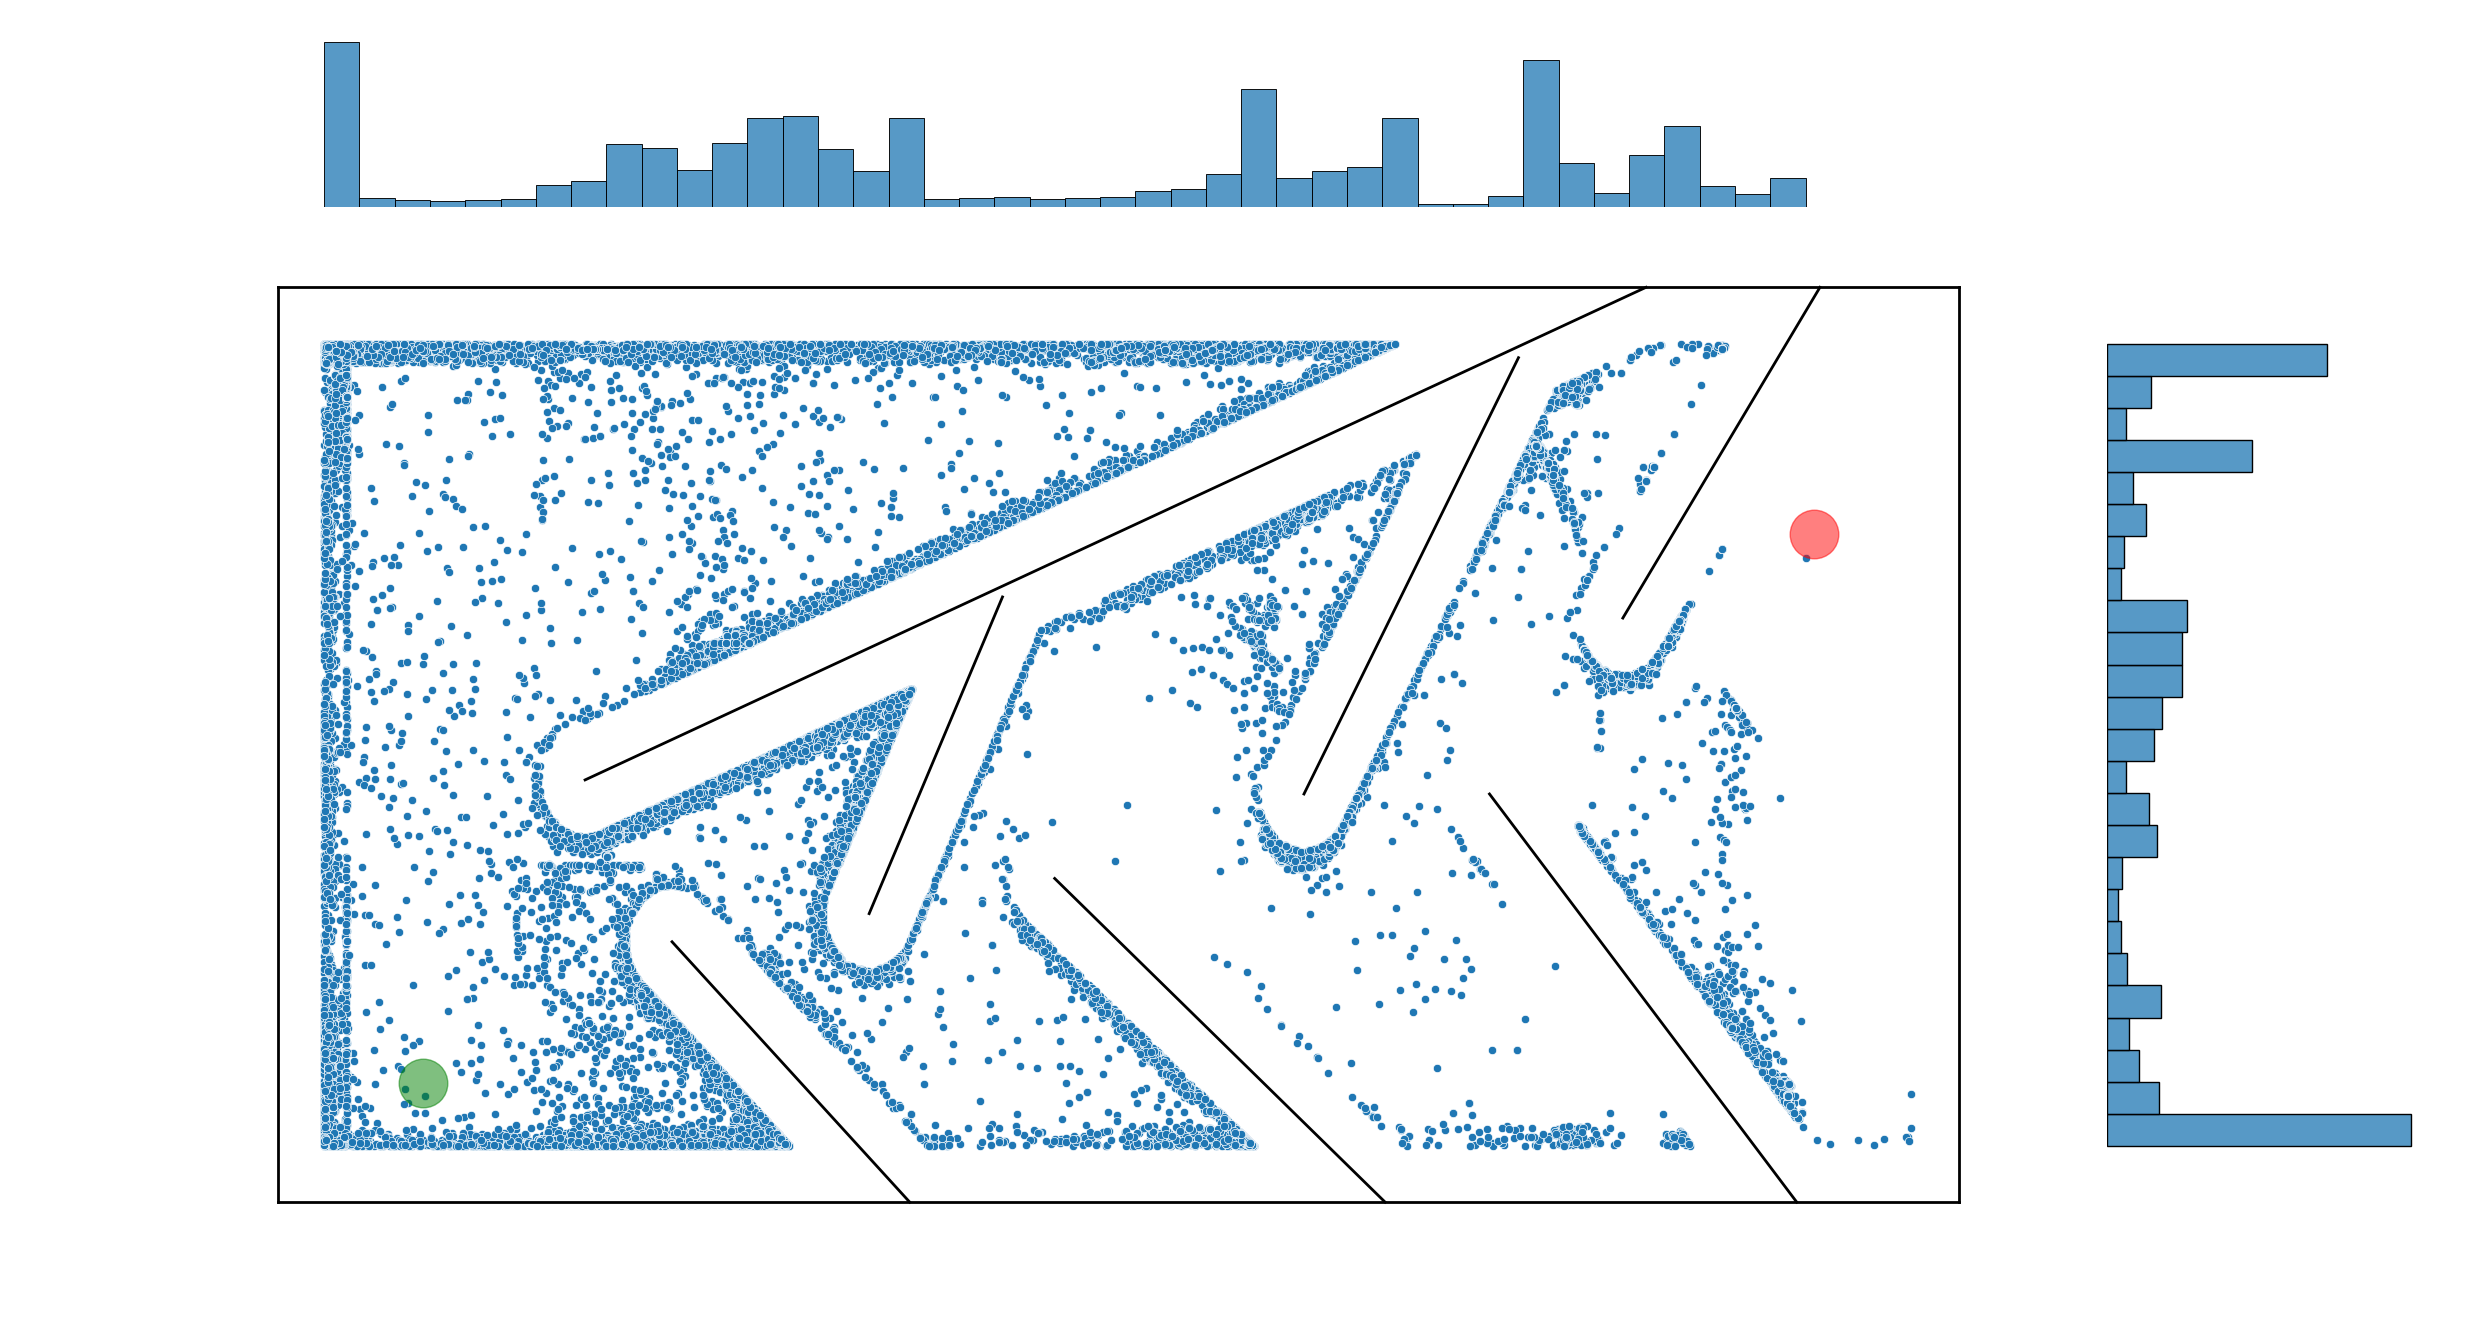
\includegraphics[scale=0.1]{resources/mazes/fitness_medium.png}
            \caption{Fitness.}
            \label{fitness_only}
        \end{subfigure}
        \begin{subfigure}[b]{0.5\textwidth}
            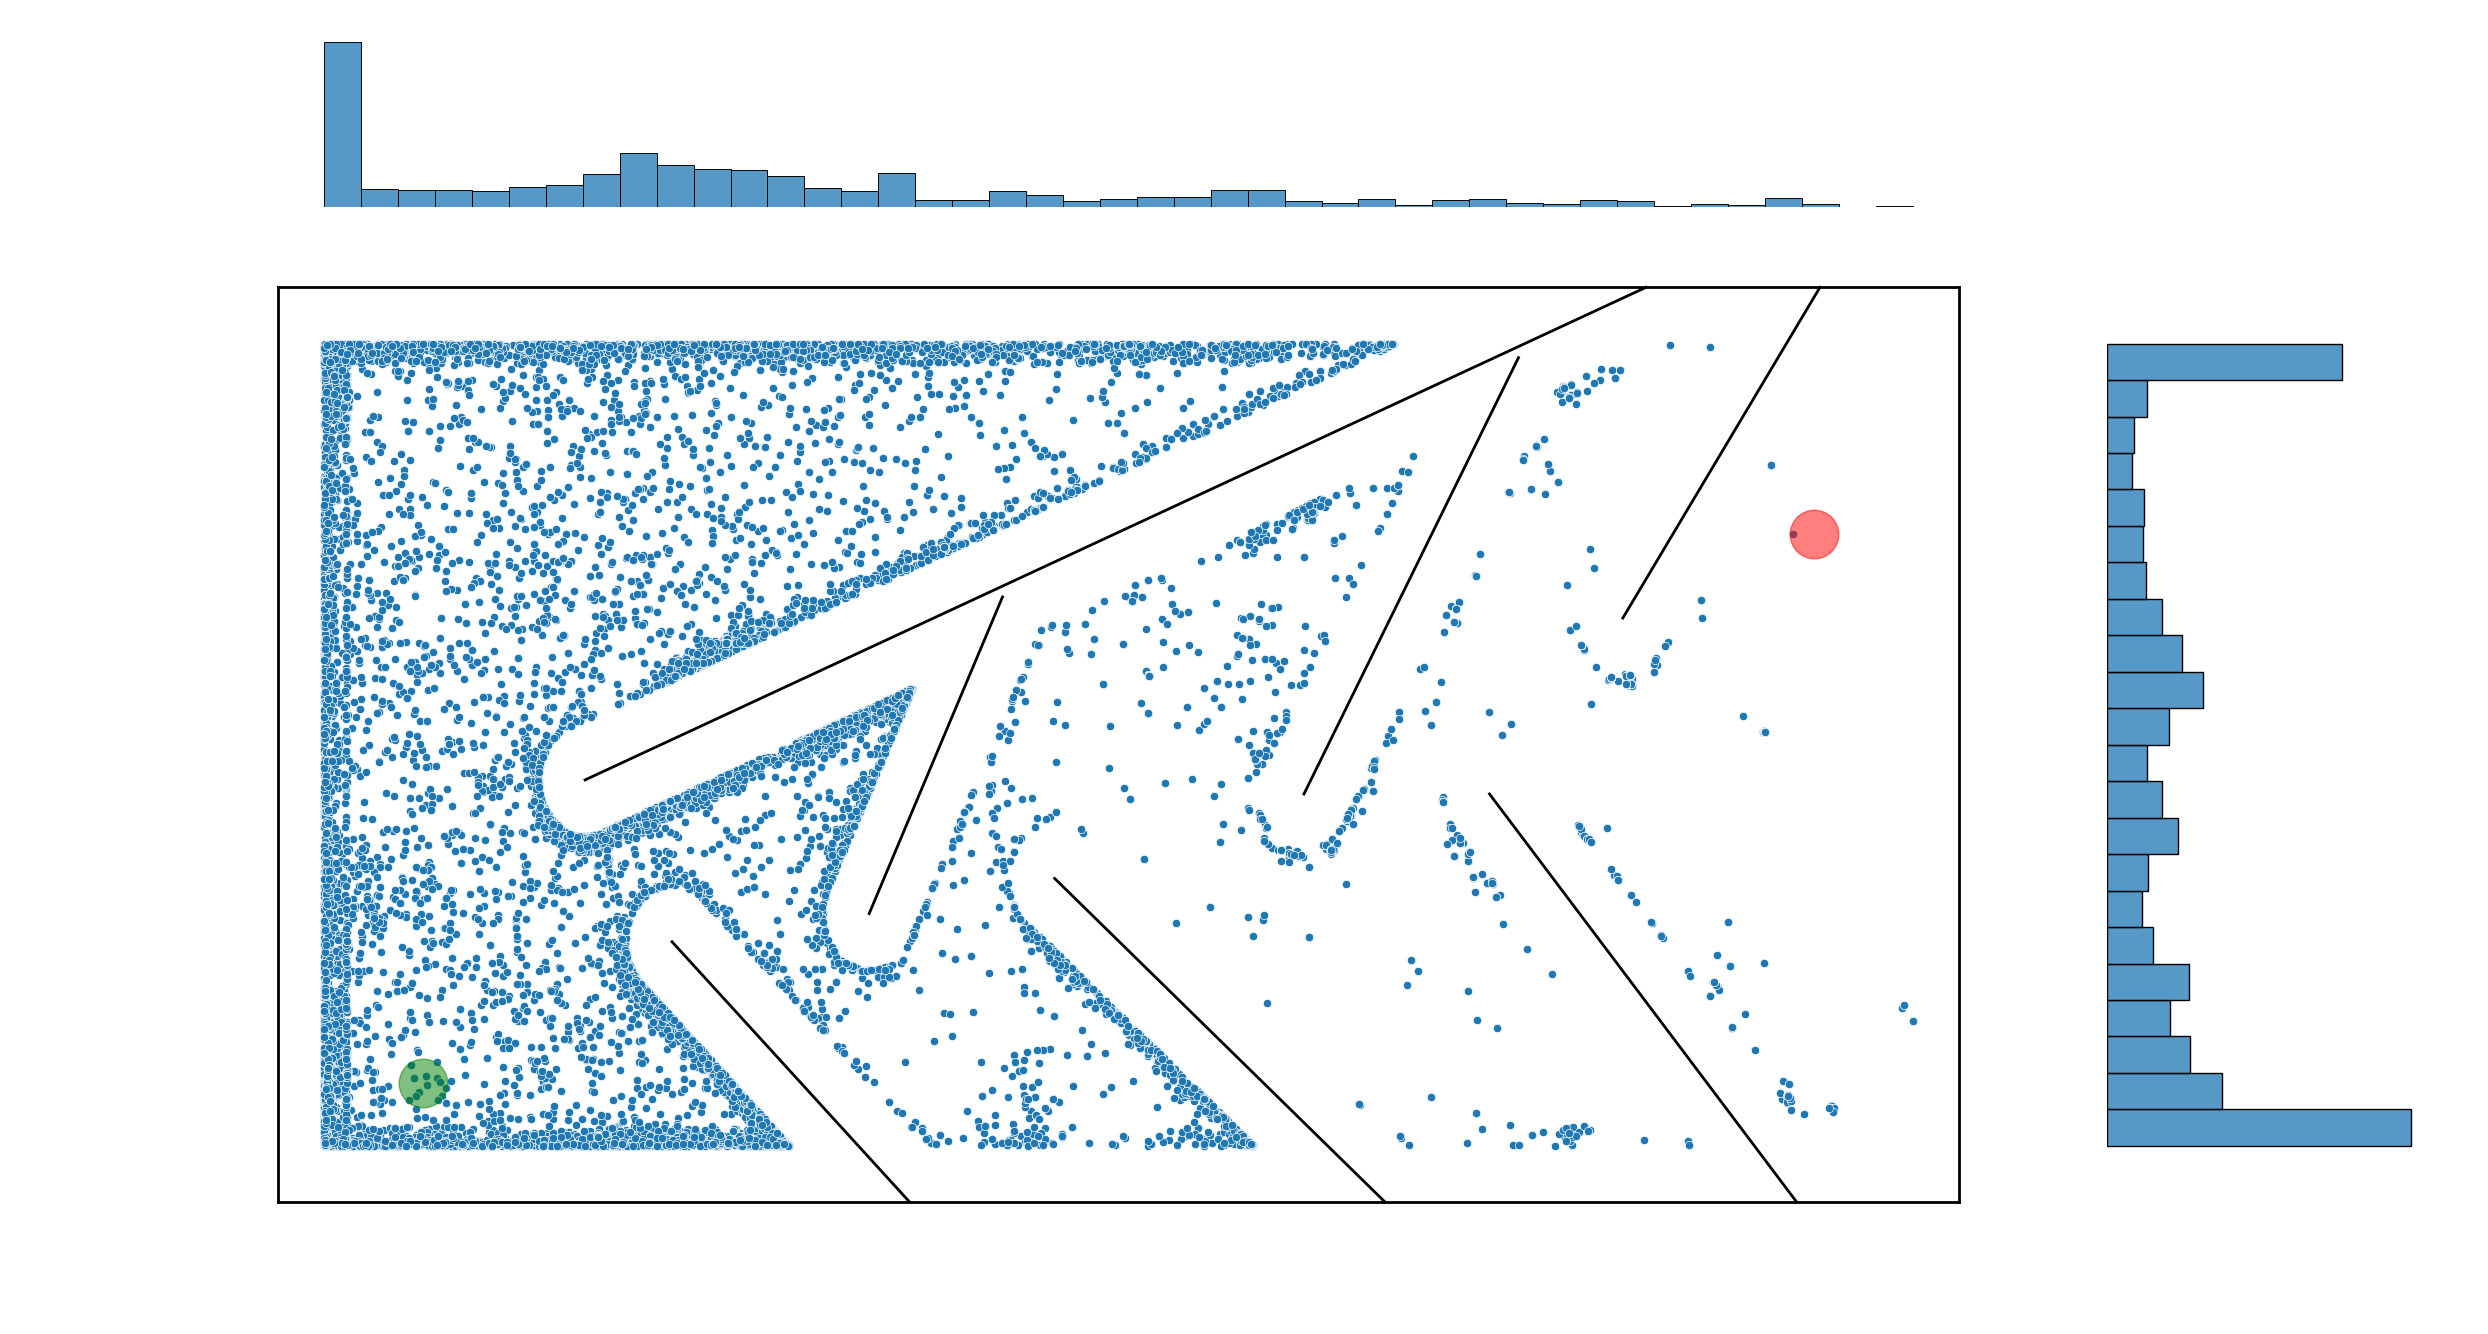
\includegraphics[scale=0.1]{resources/mazes/novelty_medium.png}
            \caption{Novelty.}
            \label{novelty_only}
        \end{subfigure}
    \end{mdframed}
    \caption{Two representative runs for fitness and novelty on the medium maze. (a) found a solution after 57811 evaluations
    and (b) found a solution after 18922 evaluations. Each point represents the final location
    of a robot after an evaluation.}
    \label{typical_runs}
\end{figure}

\subsection{Hard maze}
None of the variants were able to solve the hard maze within the $400$ time steps and $500$ generations.
The fitness rose quickly for each variant (see Figure \ref{hard_fitness}) due to the
robots entering the first dead-end. However, most of the novelty search variants
were able to quickly escape it, as indicated by the subsequent drop in fitness.
Judging from the distribution of end-points in Figure \ref{distribution}, none of the variants
were better than pure novelty search in the hard maze.

\begin{figure}[H]
    \begin{center}
        %% Creator: Matplotlib, PGF backend
%%
%% To include the figure in your LaTeX document, write
%%   \input{<filename>.pgf}
%%
%% Make sure the required packages are loaded in your preamble
%%   \usepackage{pgf}
%%
%% and, on pdftex
%%   \usepackage[utf8]{inputenc}\DeclareUnicodeCharacter{2212}{-}
%%
%% or, on luatex and xetex
%%   \usepackage{unicode-math}
%%
%% Figures using additional raster images can only be included by \input if
%% they are in the same directory as the main LaTeX file. For loading figures
%% from other directories you can use the `import` package
%%   \usepackage{import}
%%
%% and then include the figures with
%%   \import{<path to file>}{<filename>.pgf}
%%
%% Matplotlib used the following preamble
%%
\begingroup%
\makeatletter%
\begin{pgfpicture}%
\pgfpathrectangle{\pgfpointorigin}{\pgfqpoint{3.784568in}{2.909691in}}%
\pgfusepath{use as bounding box, clip}%
\begin{pgfscope}%
\pgfsetbuttcap%
\pgfsetmiterjoin%
\definecolor{currentfill}{rgb}{1.000000,1.000000,1.000000}%
\pgfsetfillcolor{currentfill}%
\pgfsetlinewidth{0.000000pt}%
\definecolor{currentstroke}{rgb}{1.000000,1.000000,1.000000}%
\pgfsetstrokecolor{currentstroke}%
\pgfsetdash{}{0pt}%
\pgfpathmoveto{\pgfqpoint{0.000000in}{0.000000in}}%
\pgfpathlineto{\pgfqpoint{3.784568in}{0.000000in}}%
\pgfpathlineto{\pgfqpoint{3.784568in}{2.909691in}}%
\pgfpathlineto{\pgfqpoint{0.000000in}{2.909691in}}%
\pgfpathclose%
\pgfusepath{fill}%
\end{pgfscope}%
\begin{pgfscope}%
\pgfsetbuttcap%
\pgfsetmiterjoin%
\definecolor{currentfill}{rgb}{1.000000,1.000000,1.000000}%
\pgfsetfillcolor{currentfill}%
\pgfsetlinewidth{0.000000pt}%
\definecolor{currentstroke}{rgb}{0.000000,0.000000,0.000000}%
\pgfsetstrokecolor{currentstroke}%
\pgfsetstrokeopacity{0.000000}%
\pgfsetdash{}{0pt}%
\pgfpathmoveto{\pgfqpoint{0.584568in}{0.499691in}}%
\pgfpathlineto{\pgfqpoint{3.684568in}{0.499691in}}%
\pgfpathlineto{\pgfqpoint{3.684568in}{2.809691in}}%
\pgfpathlineto{\pgfqpoint{0.584568in}{2.809691in}}%
\pgfpathclose%
\pgfusepath{fill}%
\end{pgfscope}%
\begin{pgfscope}%
\pgfsetbuttcap%
\pgfsetroundjoin%
\definecolor{currentfill}{rgb}{0.000000,0.000000,0.000000}%
\pgfsetfillcolor{currentfill}%
\pgfsetlinewidth{0.803000pt}%
\definecolor{currentstroke}{rgb}{0.000000,0.000000,0.000000}%
\pgfsetstrokecolor{currentstroke}%
\pgfsetdash{}{0pt}%
\pgfsys@defobject{currentmarker}{\pgfqpoint{0.000000in}{-0.048611in}}{\pgfqpoint{0.000000in}{0.000000in}}{%
\pgfpathmoveto{\pgfqpoint{0.000000in}{0.000000in}}%
\pgfpathlineto{\pgfqpoint{0.000000in}{-0.048611in}}%
\pgfusepath{stroke,fill}%
}%
\begin{pgfscope}%
\pgfsys@transformshift{0.725478in}{0.499691in}%
\pgfsys@useobject{currentmarker}{}%
\end{pgfscope}%
\end{pgfscope}%
\begin{pgfscope}%
\definecolor{textcolor}{rgb}{0.000000,0.000000,0.000000}%
\pgfsetstrokecolor{textcolor}%
\pgfsetfillcolor{textcolor}%
\pgftext[x=0.725478in,y=0.402469in,,top]{\color{textcolor}\rmfamily\fontsize{10.000000}{12.000000}\selectfont \(\displaystyle {0}\)}%
\end{pgfscope}%
\begin{pgfscope}%
\pgfsetbuttcap%
\pgfsetroundjoin%
\definecolor{currentfill}{rgb}{0.000000,0.000000,0.000000}%
\pgfsetfillcolor{currentfill}%
\pgfsetlinewidth{0.803000pt}%
\definecolor{currentstroke}{rgb}{0.000000,0.000000,0.000000}%
\pgfsetstrokecolor{currentstroke}%
\pgfsetdash{}{0pt}%
\pgfsys@defobject{currentmarker}{\pgfqpoint{0.000000in}{-0.048611in}}{\pgfqpoint{0.000000in}{0.000000in}}{%
\pgfpathmoveto{\pgfqpoint{0.000000in}{0.000000in}}%
\pgfpathlineto{\pgfqpoint{0.000000in}{-0.048611in}}%
\pgfusepath{stroke,fill}%
}%
\begin{pgfscope}%
\pgfsys@transformshift{1.290243in}{0.499691in}%
\pgfsys@useobject{currentmarker}{}%
\end{pgfscope}%
\end{pgfscope}%
\begin{pgfscope}%
\definecolor{textcolor}{rgb}{0.000000,0.000000,0.000000}%
\pgfsetstrokecolor{textcolor}%
\pgfsetfillcolor{textcolor}%
\pgftext[x=1.290243in,y=0.402469in,,top]{\color{textcolor}\rmfamily\fontsize{10.000000}{12.000000}\selectfont \(\displaystyle {100}\)}%
\end{pgfscope}%
\begin{pgfscope}%
\pgfsetbuttcap%
\pgfsetroundjoin%
\definecolor{currentfill}{rgb}{0.000000,0.000000,0.000000}%
\pgfsetfillcolor{currentfill}%
\pgfsetlinewidth{0.803000pt}%
\definecolor{currentstroke}{rgb}{0.000000,0.000000,0.000000}%
\pgfsetstrokecolor{currentstroke}%
\pgfsetdash{}{0pt}%
\pgfsys@defobject{currentmarker}{\pgfqpoint{0.000000in}{-0.048611in}}{\pgfqpoint{0.000000in}{0.000000in}}{%
\pgfpathmoveto{\pgfqpoint{0.000000in}{0.000000in}}%
\pgfpathlineto{\pgfqpoint{0.000000in}{-0.048611in}}%
\pgfusepath{stroke,fill}%
}%
\begin{pgfscope}%
\pgfsys@transformshift{1.855009in}{0.499691in}%
\pgfsys@useobject{currentmarker}{}%
\end{pgfscope}%
\end{pgfscope}%
\begin{pgfscope}%
\definecolor{textcolor}{rgb}{0.000000,0.000000,0.000000}%
\pgfsetstrokecolor{textcolor}%
\pgfsetfillcolor{textcolor}%
\pgftext[x=1.855009in,y=0.402469in,,top]{\color{textcolor}\rmfamily\fontsize{10.000000}{12.000000}\selectfont \(\displaystyle {200}\)}%
\end{pgfscope}%
\begin{pgfscope}%
\pgfsetbuttcap%
\pgfsetroundjoin%
\definecolor{currentfill}{rgb}{0.000000,0.000000,0.000000}%
\pgfsetfillcolor{currentfill}%
\pgfsetlinewidth{0.803000pt}%
\definecolor{currentstroke}{rgb}{0.000000,0.000000,0.000000}%
\pgfsetstrokecolor{currentstroke}%
\pgfsetdash{}{0pt}%
\pgfsys@defobject{currentmarker}{\pgfqpoint{0.000000in}{-0.048611in}}{\pgfqpoint{0.000000in}{0.000000in}}{%
\pgfpathmoveto{\pgfqpoint{0.000000in}{0.000000in}}%
\pgfpathlineto{\pgfqpoint{0.000000in}{-0.048611in}}%
\pgfusepath{stroke,fill}%
}%
\begin{pgfscope}%
\pgfsys@transformshift{2.419775in}{0.499691in}%
\pgfsys@useobject{currentmarker}{}%
\end{pgfscope}%
\end{pgfscope}%
\begin{pgfscope}%
\definecolor{textcolor}{rgb}{0.000000,0.000000,0.000000}%
\pgfsetstrokecolor{textcolor}%
\pgfsetfillcolor{textcolor}%
\pgftext[x=2.419775in,y=0.402469in,,top]{\color{textcolor}\rmfamily\fontsize{10.000000}{12.000000}\selectfont \(\displaystyle {300}\)}%
\end{pgfscope}%
\begin{pgfscope}%
\pgfsetbuttcap%
\pgfsetroundjoin%
\definecolor{currentfill}{rgb}{0.000000,0.000000,0.000000}%
\pgfsetfillcolor{currentfill}%
\pgfsetlinewidth{0.803000pt}%
\definecolor{currentstroke}{rgb}{0.000000,0.000000,0.000000}%
\pgfsetstrokecolor{currentstroke}%
\pgfsetdash{}{0pt}%
\pgfsys@defobject{currentmarker}{\pgfqpoint{0.000000in}{-0.048611in}}{\pgfqpoint{0.000000in}{0.000000in}}{%
\pgfpathmoveto{\pgfqpoint{0.000000in}{0.000000in}}%
\pgfpathlineto{\pgfqpoint{0.000000in}{-0.048611in}}%
\pgfusepath{stroke,fill}%
}%
\begin{pgfscope}%
\pgfsys@transformshift{2.984541in}{0.499691in}%
\pgfsys@useobject{currentmarker}{}%
\end{pgfscope}%
\end{pgfscope}%
\begin{pgfscope}%
\definecolor{textcolor}{rgb}{0.000000,0.000000,0.000000}%
\pgfsetstrokecolor{textcolor}%
\pgfsetfillcolor{textcolor}%
\pgftext[x=2.984541in,y=0.402469in,,top]{\color{textcolor}\rmfamily\fontsize{10.000000}{12.000000}\selectfont \(\displaystyle {400}\)}%
\end{pgfscope}%
\begin{pgfscope}%
\pgfsetbuttcap%
\pgfsetroundjoin%
\definecolor{currentfill}{rgb}{0.000000,0.000000,0.000000}%
\pgfsetfillcolor{currentfill}%
\pgfsetlinewidth{0.803000pt}%
\definecolor{currentstroke}{rgb}{0.000000,0.000000,0.000000}%
\pgfsetstrokecolor{currentstroke}%
\pgfsetdash{}{0pt}%
\pgfsys@defobject{currentmarker}{\pgfqpoint{0.000000in}{-0.048611in}}{\pgfqpoint{0.000000in}{0.000000in}}{%
\pgfpathmoveto{\pgfqpoint{0.000000in}{0.000000in}}%
\pgfpathlineto{\pgfqpoint{0.000000in}{-0.048611in}}%
\pgfusepath{stroke,fill}%
}%
\begin{pgfscope}%
\pgfsys@transformshift{3.549307in}{0.499691in}%
\pgfsys@useobject{currentmarker}{}%
\end{pgfscope}%
\end{pgfscope}%
\begin{pgfscope}%
\definecolor{textcolor}{rgb}{0.000000,0.000000,0.000000}%
\pgfsetstrokecolor{textcolor}%
\pgfsetfillcolor{textcolor}%
\pgftext[x=3.549307in,y=0.402469in,,top]{\color{textcolor}\rmfamily\fontsize{10.000000}{12.000000}\selectfont \(\displaystyle {500}\)}%
\end{pgfscope}%
\begin{pgfscope}%
\definecolor{textcolor}{rgb}{0.000000,0.000000,0.000000}%
\pgfsetstrokecolor{textcolor}%
\pgfsetfillcolor{textcolor}%
\pgftext[x=2.134568in,y=0.223457in,,top]{\color{textcolor}\rmfamily\fontsize{10.000000}{12.000000}\selectfont Generations}%
\end{pgfscope}%
\begin{pgfscope}%
\pgfsetbuttcap%
\pgfsetroundjoin%
\definecolor{currentfill}{rgb}{0.000000,0.000000,0.000000}%
\pgfsetfillcolor{currentfill}%
\pgfsetlinewidth{0.803000pt}%
\definecolor{currentstroke}{rgb}{0.000000,0.000000,0.000000}%
\pgfsetstrokecolor{currentstroke}%
\pgfsetdash{}{0pt}%
\pgfsys@defobject{currentmarker}{\pgfqpoint{-0.048611in}{0.000000in}}{\pgfqpoint{-0.000000in}{0.000000in}}{%
\pgfpathmoveto{\pgfqpoint{-0.000000in}{0.000000in}}%
\pgfpathlineto{\pgfqpoint{-0.048611in}{0.000000in}}%
\pgfusepath{stroke,fill}%
}%
\begin{pgfscope}%
\pgfsys@transformshift{0.584568in}{0.781836in}%
\pgfsys@useobject{currentmarker}{}%
\end{pgfscope}%
\end{pgfscope}%
\begin{pgfscope}%
\definecolor{textcolor}{rgb}{0.000000,0.000000,0.000000}%
\pgfsetstrokecolor{textcolor}%
\pgfsetfillcolor{textcolor}%
\pgftext[x=0.279012in, y=0.733610in, left, base]{\color{textcolor}\rmfamily\fontsize{10.000000}{12.000000}\selectfont \(\displaystyle {130}\)}%
\end{pgfscope}%
\begin{pgfscope}%
\pgfsetbuttcap%
\pgfsetroundjoin%
\definecolor{currentfill}{rgb}{0.000000,0.000000,0.000000}%
\pgfsetfillcolor{currentfill}%
\pgfsetlinewidth{0.803000pt}%
\definecolor{currentstroke}{rgb}{0.000000,0.000000,0.000000}%
\pgfsetstrokecolor{currentstroke}%
\pgfsetdash{}{0pt}%
\pgfsys@defobject{currentmarker}{\pgfqpoint{-0.048611in}{0.000000in}}{\pgfqpoint{-0.000000in}{0.000000in}}{%
\pgfpathmoveto{\pgfqpoint{-0.000000in}{0.000000in}}%
\pgfpathlineto{\pgfqpoint{-0.048611in}{0.000000in}}%
\pgfusepath{stroke,fill}%
}%
\begin{pgfscope}%
\pgfsys@transformshift{0.584568in}{1.094754in}%
\pgfsys@useobject{currentmarker}{}%
\end{pgfscope}%
\end{pgfscope}%
\begin{pgfscope}%
\definecolor{textcolor}{rgb}{0.000000,0.000000,0.000000}%
\pgfsetstrokecolor{textcolor}%
\pgfsetfillcolor{textcolor}%
\pgftext[x=0.279012in, y=1.046529in, left, base]{\color{textcolor}\rmfamily\fontsize{10.000000}{12.000000}\selectfont \(\displaystyle {140}\)}%
\end{pgfscope}%
\begin{pgfscope}%
\pgfsetbuttcap%
\pgfsetroundjoin%
\definecolor{currentfill}{rgb}{0.000000,0.000000,0.000000}%
\pgfsetfillcolor{currentfill}%
\pgfsetlinewidth{0.803000pt}%
\definecolor{currentstroke}{rgb}{0.000000,0.000000,0.000000}%
\pgfsetstrokecolor{currentstroke}%
\pgfsetdash{}{0pt}%
\pgfsys@defobject{currentmarker}{\pgfqpoint{-0.048611in}{0.000000in}}{\pgfqpoint{-0.000000in}{0.000000in}}{%
\pgfpathmoveto{\pgfqpoint{-0.000000in}{0.000000in}}%
\pgfpathlineto{\pgfqpoint{-0.048611in}{0.000000in}}%
\pgfusepath{stroke,fill}%
}%
\begin{pgfscope}%
\pgfsys@transformshift{0.584568in}{1.407672in}%
\pgfsys@useobject{currentmarker}{}%
\end{pgfscope}%
\end{pgfscope}%
\begin{pgfscope}%
\definecolor{textcolor}{rgb}{0.000000,0.000000,0.000000}%
\pgfsetstrokecolor{textcolor}%
\pgfsetfillcolor{textcolor}%
\pgftext[x=0.279012in, y=1.359447in, left, base]{\color{textcolor}\rmfamily\fontsize{10.000000}{12.000000}\selectfont \(\displaystyle {150}\)}%
\end{pgfscope}%
\begin{pgfscope}%
\pgfsetbuttcap%
\pgfsetroundjoin%
\definecolor{currentfill}{rgb}{0.000000,0.000000,0.000000}%
\pgfsetfillcolor{currentfill}%
\pgfsetlinewidth{0.803000pt}%
\definecolor{currentstroke}{rgb}{0.000000,0.000000,0.000000}%
\pgfsetstrokecolor{currentstroke}%
\pgfsetdash{}{0pt}%
\pgfsys@defobject{currentmarker}{\pgfqpoint{-0.048611in}{0.000000in}}{\pgfqpoint{-0.000000in}{0.000000in}}{%
\pgfpathmoveto{\pgfqpoint{-0.000000in}{0.000000in}}%
\pgfpathlineto{\pgfqpoint{-0.048611in}{0.000000in}}%
\pgfusepath{stroke,fill}%
}%
\begin{pgfscope}%
\pgfsys@transformshift{0.584568in}{1.720590in}%
\pgfsys@useobject{currentmarker}{}%
\end{pgfscope}%
\end{pgfscope}%
\begin{pgfscope}%
\definecolor{textcolor}{rgb}{0.000000,0.000000,0.000000}%
\pgfsetstrokecolor{textcolor}%
\pgfsetfillcolor{textcolor}%
\pgftext[x=0.279012in, y=1.672365in, left, base]{\color{textcolor}\rmfamily\fontsize{10.000000}{12.000000}\selectfont \(\displaystyle {160}\)}%
\end{pgfscope}%
\begin{pgfscope}%
\pgfsetbuttcap%
\pgfsetroundjoin%
\definecolor{currentfill}{rgb}{0.000000,0.000000,0.000000}%
\pgfsetfillcolor{currentfill}%
\pgfsetlinewidth{0.803000pt}%
\definecolor{currentstroke}{rgb}{0.000000,0.000000,0.000000}%
\pgfsetstrokecolor{currentstroke}%
\pgfsetdash{}{0pt}%
\pgfsys@defobject{currentmarker}{\pgfqpoint{-0.048611in}{0.000000in}}{\pgfqpoint{-0.000000in}{0.000000in}}{%
\pgfpathmoveto{\pgfqpoint{-0.000000in}{0.000000in}}%
\pgfpathlineto{\pgfqpoint{-0.048611in}{0.000000in}}%
\pgfusepath{stroke,fill}%
}%
\begin{pgfscope}%
\pgfsys@transformshift{0.584568in}{2.033508in}%
\pgfsys@useobject{currentmarker}{}%
\end{pgfscope}%
\end{pgfscope}%
\begin{pgfscope}%
\definecolor{textcolor}{rgb}{0.000000,0.000000,0.000000}%
\pgfsetstrokecolor{textcolor}%
\pgfsetfillcolor{textcolor}%
\pgftext[x=0.279012in, y=1.985283in, left, base]{\color{textcolor}\rmfamily\fontsize{10.000000}{12.000000}\selectfont \(\displaystyle {170}\)}%
\end{pgfscope}%
\begin{pgfscope}%
\pgfsetbuttcap%
\pgfsetroundjoin%
\definecolor{currentfill}{rgb}{0.000000,0.000000,0.000000}%
\pgfsetfillcolor{currentfill}%
\pgfsetlinewidth{0.803000pt}%
\definecolor{currentstroke}{rgb}{0.000000,0.000000,0.000000}%
\pgfsetstrokecolor{currentstroke}%
\pgfsetdash{}{0pt}%
\pgfsys@defobject{currentmarker}{\pgfqpoint{-0.048611in}{0.000000in}}{\pgfqpoint{-0.000000in}{0.000000in}}{%
\pgfpathmoveto{\pgfqpoint{-0.000000in}{0.000000in}}%
\pgfpathlineto{\pgfqpoint{-0.048611in}{0.000000in}}%
\pgfusepath{stroke,fill}%
}%
\begin{pgfscope}%
\pgfsys@transformshift{0.584568in}{2.346426in}%
\pgfsys@useobject{currentmarker}{}%
\end{pgfscope}%
\end{pgfscope}%
\begin{pgfscope}%
\definecolor{textcolor}{rgb}{0.000000,0.000000,0.000000}%
\pgfsetstrokecolor{textcolor}%
\pgfsetfillcolor{textcolor}%
\pgftext[x=0.279012in, y=2.298201in, left, base]{\color{textcolor}\rmfamily\fontsize{10.000000}{12.000000}\selectfont \(\displaystyle {180}\)}%
\end{pgfscope}%
\begin{pgfscope}%
\pgfsetbuttcap%
\pgfsetroundjoin%
\definecolor{currentfill}{rgb}{0.000000,0.000000,0.000000}%
\pgfsetfillcolor{currentfill}%
\pgfsetlinewidth{0.803000pt}%
\definecolor{currentstroke}{rgb}{0.000000,0.000000,0.000000}%
\pgfsetstrokecolor{currentstroke}%
\pgfsetdash{}{0pt}%
\pgfsys@defobject{currentmarker}{\pgfqpoint{-0.048611in}{0.000000in}}{\pgfqpoint{-0.000000in}{0.000000in}}{%
\pgfpathmoveto{\pgfqpoint{-0.000000in}{0.000000in}}%
\pgfpathlineto{\pgfqpoint{-0.048611in}{0.000000in}}%
\pgfusepath{stroke,fill}%
}%
\begin{pgfscope}%
\pgfsys@transformshift{0.584568in}{2.659345in}%
\pgfsys@useobject{currentmarker}{}%
\end{pgfscope}%
\end{pgfscope}%
\begin{pgfscope}%
\definecolor{textcolor}{rgb}{0.000000,0.000000,0.000000}%
\pgfsetstrokecolor{textcolor}%
\pgfsetfillcolor{textcolor}%
\pgftext[x=0.279012in, y=2.611119in, left, base]{\color{textcolor}\rmfamily\fontsize{10.000000}{12.000000}\selectfont \(\displaystyle {190}\)}%
\end{pgfscope}%
\begin{pgfscope}%
\definecolor{textcolor}{rgb}{0.000000,0.000000,0.000000}%
\pgfsetstrokecolor{textcolor}%
\pgfsetfillcolor{textcolor}%
\pgftext[x=0.223457in,y=1.654691in,,bottom,rotate=90.000000]{\color{textcolor}\rmfamily\fontsize{10.000000}{12.000000}\selectfont Average fitness}%
\end{pgfscope}%
\begin{pgfscope}%
\pgfpathrectangle{\pgfqpoint{0.584568in}{0.499691in}}{\pgfqpoint{3.100000in}{2.310000in}}%
\pgfusepath{clip}%
\pgfsetrectcap%
\pgfsetroundjoin%
\pgfsetlinewidth{1.505625pt}%
\definecolor{currentstroke}{rgb}{0.121569,0.466667,0.705882}%
\pgfsetstrokecolor{currentstroke}%
\pgfsetdash{}{0pt}%
\pgfpathmoveto{\pgfqpoint{0.725478in}{0.695482in}}%
\pgfpathlineto{\pgfqpoint{0.731125in}{0.940833in}}%
\pgfpathlineto{\pgfqpoint{0.736773in}{1.130318in}}%
\pgfpathlineto{\pgfqpoint{0.742421in}{1.188738in}}%
\pgfpathlineto{\pgfqpoint{0.753716in}{1.540930in}}%
\pgfpathlineto{\pgfqpoint{0.759364in}{1.674265in}}%
\pgfpathlineto{\pgfqpoint{0.765011in}{1.758514in}}%
\pgfpathlineto{\pgfqpoint{0.770659in}{1.860399in}}%
\pgfpathlineto{\pgfqpoint{0.776306in}{1.914777in}}%
\pgfpathlineto{\pgfqpoint{0.781954in}{1.998294in}}%
\pgfpathlineto{\pgfqpoint{0.787602in}{2.012449in}}%
\pgfpathlineto{\pgfqpoint{0.793249in}{2.003353in}}%
\pgfpathlineto{\pgfqpoint{0.798897in}{2.059601in}}%
\pgfpathlineto{\pgfqpoint{0.804545in}{2.093998in}}%
\pgfpathlineto{\pgfqpoint{0.810192in}{2.109531in}}%
\pgfpathlineto{\pgfqpoint{0.815840in}{2.129653in}}%
\pgfpathlineto{\pgfqpoint{0.821488in}{2.168402in}}%
\pgfpathlineto{\pgfqpoint{0.827135in}{2.173782in}}%
\pgfpathlineto{\pgfqpoint{0.832783in}{2.190680in}}%
\pgfpathlineto{\pgfqpoint{0.838431in}{2.230556in}}%
\pgfpathlineto{\pgfqpoint{0.844078in}{2.224967in}}%
\pgfpathlineto{\pgfqpoint{0.849726in}{2.242541in}}%
\pgfpathlineto{\pgfqpoint{0.855374in}{2.264163in}}%
\pgfpathlineto{\pgfqpoint{0.861021in}{2.258471in}}%
\pgfpathlineto{\pgfqpoint{0.872317in}{2.241777in}}%
\pgfpathlineto{\pgfqpoint{0.877964in}{2.277620in}}%
\pgfpathlineto{\pgfqpoint{0.883612in}{2.231467in}}%
\pgfpathlineto{\pgfqpoint{0.889260in}{2.281683in}}%
\pgfpathlineto{\pgfqpoint{0.894907in}{2.289706in}}%
\pgfpathlineto{\pgfqpoint{0.900555in}{2.282040in}}%
\pgfpathlineto{\pgfqpoint{0.906203in}{2.283726in}}%
\pgfpathlineto{\pgfqpoint{0.911850in}{2.296724in}}%
\pgfpathlineto{\pgfqpoint{0.917498in}{2.242561in}}%
\pgfpathlineto{\pgfqpoint{0.923146in}{2.297141in}}%
\pgfpathlineto{\pgfqpoint{0.928793in}{2.316756in}}%
\pgfpathlineto{\pgfqpoint{0.934441in}{2.296592in}}%
\pgfpathlineto{\pgfqpoint{0.940089in}{2.331658in}}%
\pgfpathlineto{\pgfqpoint{0.945736in}{2.314237in}}%
\pgfpathlineto{\pgfqpoint{0.951384in}{2.365833in}}%
\pgfpathlineto{\pgfqpoint{0.957032in}{2.342331in}}%
\pgfpathlineto{\pgfqpoint{0.962679in}{2.325852in}}%
\pgfpathlineto{\pgfqpoint{0.968327in}{2.350544in}}%
\pgfpathlineto{\pgfqpoint{0.973975in}{2.321907in}}%
\pgfpathlineto{\pgfqpoint{0.979622in}{2.337134in}}%
\pgfpathlineto{\pgfqpoint{0.985270in}{2.356457in}}%
\pgfpathlineto{\pgfqpoint{0.990918in}{2.347920in}}%
\pgfpathlineto{\pgfqpoint{0.996565in}{2.360767in}}%
\pgfpathlineto{\pgfqpoint{1.002213in}{2.380508in}}%
\pgfpathlineto{\pgfqpoint{1.007861in}{2.355674in}}%
\pgfpathlineto{\pgfqpoint{1.013508in}{2.366418in}}%
\pgfpathlineto{\pgfqpoint{1.019156in}{2.372665in}}%
\pgfpathlineto{\pgfqpoint{1.024803in}{2.363924in}}%
\pgfpathlineto{\pgfqpoint{1.036099in}{2.383570in}}%
\pgfpathlineto{\pgfqpoint{1.041746in}{2.367525in}}%
\pgfpathlineto{\pgfqpoint{1.047394in}{2.372454in}}%
\pgfpathlineto{\pgfqpoint{1.053042in}{2.394249in}}%
\pgfpathlineto{\pgfqpoint{1.058689in}{2.435000in}}%
\pgfpathlineto{\pgfqpoint{1.064337in}{2.414444in}}%
\pgfpathlineto{\pgfqpoint{1.069985in}{2.429151in}}%
\pgfpathlineto{\pgfqpoint{1.075632in}{2.366802in}}%
\pgfpathlineto{\pgfqpoint{1.081280in}{2.406658in}}%
\pgfpathlineto{\pgfqpoint{1.086928in}{2.393892in}}%
\pgfpathlineto{\pgfqpoint{1.092575in}{2.428907in}}%
\pgfpathlineto{\pgfqpoint{1.098223in}{2.410616in}}%
\pgfpathlineto{\pgfqpoint{1.103871in}{2.437669in}}%
\pgfpathlineto{\pgfqpoint{1.109518in}{2.472307in}}%
\pgfpathlineto{\pgfqpoint{1.115166in}{2.474205in}}%
\pgfpathlineto{\pgfqpoint{1.120814in}{2.461677in}}%
\pgfpathlineto{\pgfqpoint{1.126461in}{2.452048in}}%
\pgfpathlineto{\pgfqpoint{1.132109in}{2.476471in}}%
\pgfpathlineto{\pgfqpoint{1.137757in}{2.434533in}}%
\pgfpathlineto{\pgfqpoint{1.143404in}{2.465901in}}%
\pgfpathlineto{\pgfqpoint{1.149052in}{2.477414in}}%
\pgfpathlineto{\pgfqpoint{1.154700in}{2.452073in}}%
\pgfpathlineto{\pgfqpoint{1.160347in}{2.470169in}}%
\pgfpathlineto{\pgfqpoint{1.165995in}{2.478575in}}%
\pgfpathlineto{\pgfqpoint{1.177290in}{2.469221in}}%
\pgfpathlineto{\pgfqpoint{1.182938in}{2.488047in}}%
\pgfpathlineto{\pgfqpoint{1.188586in}{2.448983in}}%
\pgfpathlineto{\pgfqpoint{1.194233in}{2.458118in}}%
\pgfpathlineto{\pgfqpoint{1.199881in}{2.484840in}}%
\pgfpathlineto{\pgfqpoint{1.205529in}{2.498849in}}%
\pgfpathlineto{\pgfqpoint{1.211176in}{2.467437in}}%
\pgfpathlineto{\pgfqpoint{1.216824in}{2.465269in}}%
\pgfpathlineto{\pgfqpoint{1.222472in}{2.488599in}}%
\pgfpathlineto{\pgfqpoint{1.228119in}{2.466060in}}%
\pgfpathlineto{\pgfqpoint{1.233767in}{2.487481in}}%
\pgfpathlineto{\pgfqpoint{1.239415in}{2.464364in}}%
\pgfpathlineto{\pgfqpoint{1.250710in}{2.470445in}}%
\pgfpathlineto{\pgfqpoint{1.256358in}{2.480114in}}%
\pgfpathlineto{\pgfqpoint{1.262005in}{2.485449in}}%
\pgfpathlineto{\pgfqpoint{1.267653in}{2.471074in}}%
\pgfpathlineto{\pgfqpoint{1.273300in}{2.497919in}}%
\pgfpathlineto{\pgfqpoint{1.278948in}{2.483875in}}%
\pgfpathlineto{\pgfqpoint{1.284596in}{2.483409in}}%
\pgfpathlineto{\pgfqpoint{1.290243in}{2.513022in}}%
\pgfpathlineto{\pgfqpoint{1.295891in}{2.503175in}}%
\pgfpathlineto{\pgfqpoint{1.301539in}{2.502157in}}%
\pgfpathlineto{\pgfqpoint{1.307186in}{2.510711in}}%
\pgfpathlineto{\pgfqpoint{1.312834in}{2.507519in}}%
\pgfpathlineto{\pgfqpoint{1.318482in}{2.445814in}}%
\pgfpathlineto{\pgfqpoint{1.324129in}{2.482599in}}%
\pgfpathlineto{\pgfqpoint{1.329777in}{2.477536in}}%
\pgfpathlineto{\pgfqpoint{1.335425in}{2.448267in}}%
\pgfpathlineto{\pgfqpoint{1.341072in}{2.491777in}}%
\pgfpathlineto{\pgfqpoint{1.346720in}{2.487061in}}%
\pgfpathlineto{\pgfqpoint{1.352368in}{2.533347in}}%
\pgfpathlineto{\pgfqpoint{1.358015in}{2.494543in}}%
\pgfpathlineto{\pgfqpoint{1.363663in}{2.532282in}}%
\pgfpathlineto{\pgfqpoint{1.369311in}{2.523775in}}%
\pgfpathlineto{\pgfqpoint{1.374958in}{2.543488in}}%
\pgfpathlineto{\pgfqpoint{1.380606in}{2.521058in}}%
\pgfpathlineto{\pgfqpoint{1.386254in}{2.515848in}}%
\pgfpathlineto{\pgfqpoint{1.391901in}{2.515061in}}%
\pgfpathlineto{\pgfqpoint{1.397549in}{2.483203in}}%
\pgfpathlineto{\pgfqpoint{1.403197in}{2.518076in}}%
\pgfpathlineto{\pgfqpoint{1.408844in}{2.536708in}}%
\pgfpathlineto{\pgfqpoint{1.414492in}{2.511111in}}%
\pgfpathlineto{\pgfqpoint{1.420140in}{2.527840in}}%
\pgfpathlineto{\pgfqpoint{1.425787in}{2.566949in}}%
\pgfpathlineto{\pgfqpoint{1.431435in}{2.537668in}}%
\pgfpathlineto{\pgfqpoint{1.437083in}{2.490995in}}%
\pgfpathlineto{\pgfqpoint{1.442730in}{2.503541in}}%
\pgfpathlineto{\pgfqpoint{1.448378in}{2.549902in}}%
\pgfpathlineto{\pgfqpoint{1.454026in}{2.542720in}}%
\pgfpathlineto{\pgfqpoint{1.459673in}{2.578796in}}%
\pgfpathlineto{\pgfqpoint{1.465321in}{2.544300in}}%
\pgfpathlineto{\pgfqpoint{1.470969in}{2.558804in}}%
\pgfpathlineto{\pgfqpoint{1.476616in}{2.580282in}}%
\pgfpathlineto{\pgfqpoint{1.482264in}{2.541434in}}%
\pgfpathlineto{\pgfqpoint{1.487912in}{2.591836in}}%
\pgfpathlineto{\pgfqpoint{1.493559in}{2.530770in}}%
\pgfpathlineto{\pgfqpoint{1.499207in}{2.546394in}}%
\pgfpathlineto{\pgfqpoint{1.504854in}{2.532375in}}%
\pgfpathlineto{\pgfqpoint{1.510502in}{2.551585in}}%
\pgfpathlineto{\pgfqpoint{1.516150in}{2.528431in}}%
\pgfpathlineto{\pgfqpoint{1.521797in}{2.542769in}}%
\pgfpathlineto{\pgfqpoint{1.527445in}{2.586827in}}%
\pgfpathlineto{\pgfqpoint{1.533093in}{2.549790in}}%
\pgfpathlineto{\pgfqpoint{1.538740in}{2.545760in}}%
\pgfpathlineto{\pgfqpoint{1.550036in}{2.550023in}}%
\pgfpathlineto{\pgfqpoint{1.555683in}{2.553251in}}%
\pgfpathlineto{\pgfqpoint{1.561331in}{2.552438in}}%
\pgfpathlineto{\pgfqpoint{1.566979in}{2.561661in}}%
\pgfpathlineto{\pgfqpoint{1.572626in}{2.557923in}}%
\pgfpathlineto{\pgfqpoint{1.578274in}{2.560657in}}%
\pgfpathlineto{\pgfqpoint{1.583922in}{2.557662in}}%
\pgfpathlineto{\pgfqpoint{1.589569in}{2.573539in}}%
\pgfpathlineto{\pgfqpoint{1.595217in}{2.557143in}}%
\pgfpathlineto{\pgfqpoint{1.600865in}{2.591081in}}%
\pgfpathlineto{\pgfqpoint{1.606512in}{2.589734in}}%
\pgfpathlineto{\pgfqpoint{1.612160in}{2.595346in}}%
\pgfpathlineto{\pgfqpoint{1.617808in}{2.547046in}}%
\pgfpathlineto{\pgfqpoint{1.623455in}{2.584319in}}%
\pgfpathlineto{\pgfqpoint{1.634751in}{2.547046in}}%
\pgfpathlineto{\pgfqpoint{1.640398in}{2.602635in}}%
\pgfpathlineto{\pgfqpoint{1.646046in}{2.575570in}}%
\pgfpathlineto{\pgfqpoint{1.651694in}{2.573188in}}%
\pgfpathlineto{\pgfqpoint{1.657341in}{2.611519in}}%
\pgfpathlineto{\pgfqpoint{1.662989in}{2.568980in}}%
\pgfpathlineto{\pgfqpoint{1.668637in}{2.550080in}}%
\pgfpathlineto{\pgfqpoint{1.674284in}{2.588314in}}%
\pgfpathlineto{\pgfqpoint{1.679932in}{2.595675in}}%
\pgfpathlineto{\pgfqpoint{1.685580in}{2.558647in}}%
\pgfpathlineto{\pgfqpoint{1.691227in}{2.560378in}}%
\pgfpathlineto{\pgfqpoint{1.696875in}{2.612251in}}%
\pgfpathlineto{\pgfqpoint{1.702523in}{2.587679in}}%
\pgfpathlineto{\pgfqpoint{1.708170in}{2.572390in}}%
\pgfpathlineto{\pgfqpoint{1.713818in}{2.575005in}}%
\pgfpathlineto{\pgfqpoint{1.719466in}{2.590451in}}%
\pgfpathlineto{\pgfqpoint{1.725113in}{2.586929in}}%
\pgfpathlineto{\pgfqpoint{1.730761in}{2.577200in}}%
\pgfpathlineto{\pgfqpoint{1.742056in}{2.610606in}}%
\pgfpathlineto{\pgfqpoint{1.747704in}{2.602567in}}%
\pgfpathlineto{\pgfqpoint{1.753351in}{2.643669in}}%
\pgfpathlineto{\pgfqpoint{1.758999in}{2.618303in}}%
\pgfpathlineto{\pgfqpoint{1.764647in}{2.601739in}}%
\pgfpathlineto{\pgfqpoint{1.775942in}{2.617622in}}%
\pgfpathlineto{\pgfqpoint{1.781590in}{2.579007in}}%
\pgfpathlineto{\pgfqpoint{1.787237in}{2.591586in}}%
\pgfpathlineto{\pgfqpoint{1.792885in}{2.590624in}}%
\pgfpathlineto{\pgfqpoint{1.798533in}{2.577440in}}%
\pgfpathlineto{\pgfqpoint{1.804180in}{2.581858in}}%
\pgfpathlineto{\pgfqpoint{1.809828in}{2.592119in}}%
\pgfpathlineto{\pgfqpoint{1.815476in}{2.611232in}}%
\pgfpathlineto{\pgfqpoint{1.821123in}{2.589434in}}%
\pgfpathlineto{\pgfqpoint{1.826771in}{2.604824in}}%
\pgfpathlineto{\pgfqpoint{1.832419in}{2.595387in}}%
\pgfpathlineto{\pgfqpoint{1.838066in}{2.595506in}}%
\pgfpathlineto{\pgfqpoint{1.843714in}{2.663066in}}%
\pgfpathlineto{\pgfqpoint{1.849362in}{2.619494in}}%
\pgfpathlineto{\pgfqpoint{1.855009in}{2.633520in}}%
\pgfpathlineto{\pgfqpoint{1.860657in}{2.612256in}}%
\pgfpathlineto{\pgfqpoint{1.866305in}{2.615253in}}%
\pgfpathlineto{\pgfqpoint{1.871952in}{2.648494in}}%
\pgfpathlineto{\pgfqpoint{1.877600in}{2.641976in}}%
\pgfpathlineto{\pgfqpoint{1.883248in}{2.657506in}}%
\pgfpathlineto{\pgfqpoint{1.888895in}{2.640079in}}%
\pgfpathlineto{\pgfqpoint{1.894543in}{2.617491in}}%
\pgfpathlineto{\pgfqpoint{1.900191in}{2.650187in}}%
\pgfpathlineto{\pgfqpoint{1.905838in}{2.651103in}}%
\pgfpathlineto{\pgfqpoint{1.911486in}{2.630254in}}%
\pgfpathlineto{\pgfqpoint{1.917134in}{2.618940in}}%
\pgfpathlineto{\pgfqpoint{1.922781in}{2.617384in}}%
\pgfpathlineto{\pgfqpoint{1.928429in}{2.602105in}}%
\pgfpathlineto{\pgfqpoint{1.934077in}{2.642720in}}%
\pgfpathlineto{\pgfqpoint{1.939724in}{2.647848in}}%
\pgfpathlineto{\pgfqpoint{1.945372in}{2.598502in}}%
\pgfpathlineto{\pgfqpoint{1.951020in}{2.644170in}}%
\pgfpathlineto{\pgfqpoint{1.956667in}{2.631084in}}%
\pgfpathlineto{\pgfqpoint{1.962315in}{2.638025in}}%
\pgfpathlineto{\pgfqpoint{1.967963in}{2.624149in}}%
\pgfpathlineto{\pgfqpoint{1.973610in}{2.632395in}}%
\pgfpathlineto{\pgfqpoint{1.979258in}{2.627691in}}%
\pgfpathlineto{\pgfqpoint{1.984906in}{2.631426in}}%
\pgfpathlineto{\pgfqpoint{1.990553in}{2.611034in}}%
\pgfpathlineto{\pgfqpoint{1.996201in}{2.643598in}}%
\pgfpathlineto{\pgfqpoint{2.001848in}{2.632155in}}%
\pgfpathlineto{\pgfqpoint{2.007496in}{2.629832in}}%
\pgfpathlineto{\pgfqpoint{2.013144in}{2.635247in}}%
\pgfpathlineto{\pgfqpoint{2.018791in}{2.624654in}}%
\pgfpathlineto{\pgfqpoint{2.024439in}{2.670616in}}%
\pgfpathlineto{\pgfqpoint{2.030087in}{2.648210in}}%
\pgfpathlineto{\pgfqpoint{2.035734in}{2.656010in}}%
\pgfpathlineto{\pgfqpoint{2.041382in}{2.671675in}}%
\pgfpathlineto{\pgfqpoint{2.047030in}{2.634730in}}%
\pgfpathlineto{\pgfqpoint{2.052677in}{2.639515in}}%
\pgfpathlineto{\pgfqpoint{2.058325in}{2.627832in}}%
\pgfpathlineto{\pgfqpoint{2.063973in}{2.627589in}}%
\pgfpathlineto{\pgfqpoint{2.069620in}{2.614254in}}%
\pgfpathlineto{\pgfqpoint{2.080916in}{2.680199in}}%
\pgfpathlineto{\pgfqpoint{2.086563in}{2.659026in}}%
\pgfpathlineto{\pgfqpoint{2.092211in}{2.652002in}}%
\pgfpathlineto{\pgfqpoint{2.097859in}{2.648626in}}%
\pgfpathlineto{\pgfqpoint{2.103506in}{2.658298in}}%
\pgfpathlineto{\pgfqpoint{2.109154in}{2.601601in}}%
\pgfpathlineto{\pgfqpoint{2.114802in}{2.633366in}}%
\pgfpathlineto{\pgfqpoint{2.120449in}{2.641301in}}%
\pgfpathlineto{\pgfqpoint{2.126097in}{2.618062in}}%
\pgfpathlineto{\pgfqpoint{2.131745in}{2.579325in}}%
\pgfpathlineto{\pgfqpoint{2.137392in}{2.642791in}}%
\pgfpathlineto{\pgfqpoint{2.143040in}{2.660287in}}%
\pgfpathlineto{\pgfqpoint{2.148688in}{2.630110in}}%
\pgfpathlineto{\pgfqpoint{2.154335in}{2.625418in}}%
\pgfpathlineto{\pgfqpoint{2.165631in}{2.662916in}}%
\pgfpathlineto{\pgfqpoint{2.171278in}{2.621510in}}%
\pgfpathlineto{\pgfqpoint{2.176926in}{2.642072in}}%
\pgfpathlineto{\pgfqpoint{2.182574in}{2.671234in}}%
\pgfpathlineto{\pgfqpoint{2.188221in}{2.661738in}}%
\pgfpathlineto{\pgfqpoint{2.193869in}{2.658929in}}%
\pgfpathlineto{\pgfqpoint{2.199517in}{2.679783in}}%
\pgfpathlineto{\pgfqpoint{2.205164in}{2.616945in}}%
\pgfpathlineto{\pgfqpoint{2.210812in}{2.617419in}}%
\pgfpathlineto{\pgfqpoint{2.216460in}{2.641678in}}%
\pgfpathlineto{\pgfqpoint{2.222107in}{2.615096in}}%
\pgfpathlineto{\pgfqpoint{2.227755in}{2.630734in}}%
\pgfpathlineto{\pgfqpoint{2.233403in}{2.636680in}}%
\pgfpathlineto{\pgfqpoint{2.239050in}{2.648786in}}%
\pgfpathlineto{\pgfqpoint{2.244698in}{2.630302in}}%
\pgfpathlineto{\pgfqpoint{2.250345in}{2.660434in}}%
\pgfpathlineto{\pgfqpoint{2.255993in}{2.666002in}}%
\pgfpathlineto{\pgfqpoint{2.261641in}{2.674515in}}%
\pgfpathlineto{\pgfqpoint{2.267288in}{2.616583in}}%
\pgfpathlineto{\pgfqpoint{2.272936in}{2.648668in}}%
\pgfpathlineto{\pgfqpoint{2.278584in}{2.619475in}}%
\pgfpathlineto{\pgfqpoint{2.284231in}{2.664718in}}%
\pgfpathlineto{\pgfqpoint{2.289879in}{2.633564in}}%
\pgfpathlineto{\pgfqpoint{2.295527in}{2.629699in}}%
\pgfpathlineto{\pgfqpoint{2.301174in}{2.632549in}}%
\pgfpathlineto{\pgfqpoint{2.306822in}{2.607742in}}%
\pgfpathlineto{\pgfqpoint{2.312470in}{2.655886in}}%
\pgfpathlineto{\pgfqpoint{2.318117in}{2.620133in}}%
\pgfpathlineto{\pgfqpoint{2.323765in}{2.649830in}}%
\pgfpathlineto{\pgfqpoint{2.329413in}{2.669699in}}%
\pgfpathlineto{\pgfqpoint{2.335060in}{2.629928in}}%
\pgfpathlineto{\pgfqpoint{2.340708in}{2.630690in}}%
\pgfpathlineto{\pgfqpoint{2.346356in}{2.636013in}}%
\pgfpathlineto{\pgfqpoint{2.352003in}{2.637651in}}%
\pgfpathlineto{\pgfqpoint{2.357651in}{2.675720in}}%
\pgfpathlineto{\pgfqpoint{2.363299in}{2.611584in}}%
\pgfpathlineto{\pgfqpoint{2.374594in}{2.682782in}}%
\pgfpathlineto{\pgfqpoint{2.380242in}{2.668442in}}%
\pgfpathlineto{\pgfqpoint{2.385889in}{2.697478in}}%
\pgfpathlineto{\pgfqpoint{2.391537in}{2.662360in}}%
\pgfpathlineto{\pgfqpoint{2.402832in}{2.657473in}}%
\pgfpathlineto{\pgfqpoint{2.408480in}{2.642511in}}%
\pgfpathlineto{\pgfqpoint{2.414128in}{2.643930in}}%
\pgfpathlineto{\pgfqpoint{2.419775in}{2.642845in}}%
\pgfpathlineto{\pgfqpoint{2.425423in}{2.643801in}}%
\pgfpathlineto{\pgfqpoint{2.431071in}{2.620634in}}%
\pgfpathlineto{\pgfqpoint{2.436718in}{2.645646in}}%
\pgfpathlineto{\pgfqpoint{2.442366in}{2.631305in}}%
\pgfpathlineto{\pgfqpoint{2.448014in}{2.630964in}}%
\pgfpathlineto{\pgfqpoint{2.453661in}{2.622576in}}%
\pgfpathlineto{\pgfqpoint{2.464957in}{2.671473in}}%
\pgfpathlineto{\pgfqpoint{2.470604in}{2.623558in}}%
\pgfpathlineto{\pgfqpoint{2.476252in}{2.671396in}}%
\pgfpathlineto{\pgfqpoint{2.481899in}{2.680359in}}%
\pgfpathlineto{\pgfqpoint{2.487547in}{2.668012in}}%
\pgfpathlineto{\pgfqpoint{2.493195in}{2.668110in}}%
\pgfpathlineto{\pgfqpoint{2.498842in}{2.679822in}}%
\pgfpathlineto{\pgfqpoint{2.504490in}{2.656405in}}%
\pgfpathlineto{\pgfqpoint{2.510138in}{2.667587in}}%
\pgfpathlineto{\pgfqpoint{2.515785in}{2.648161in}}%
\pgfpathlineto{\pgfqpoint{2.521433in}{2.678408in}}%
\pgfpathlineto{\pgfqpoint{2.527081in}{2.642735in}}%
\pgfpathlineto{\pgfqpoint{2.532728in}{2.677509in}}%
\pgfpathlineto{\pgfqpoint{2.538376in}{2.653708in}}%
\pgfpathlineto{\pgfqpoint{2.544024in}{2.654847in}}%
\pgfpathlineto{\pgfqpoint{2.549671in}{2.609927in}}%
\pgfpathlineto{\pgfqpoint{2.555319in}{2.648005in}}%
\pgfpathlineto{\pgfqpoint{2.566614in}{2.660322in}}%
\pgfpathlineto{\pgfqpoint{2.572262in}{2.666694in}}%
\pgfpathlineto{\pgfqpoint{2.577910in}{2.635987in}}%
\pgfpathlineto{\pgfqpoint{2.583557in}{2.628033in}}%
\pgfpathlineto{\pgfqpoint{2.589205in}{2.629053in}}%
\pgfpathlineto{\pgfqpoint{2.594853in}{2.597248in}}%
\pgfpathlineto{\pgfqpoint{2.600500in}{2.633999in}}%
\pgfpathlineto{\pgfqpoint{2.606148in}{2.614808in}}%
\pgfpathlineto{\pgfqpoint{2.611796in}{2.644982in}}%
\pgfpathlineto{\pgfqpoint{2.617443in}{2.627824in}}%
\pgfpathlineto{\pgfqpoint{2.623091in}{2.641787in}}%
\pgfpathlineto{\pgfqpoint{2.628739in}{2.644990in}}%
\pgfpathlineto{\pgfqpoint{2.634386in}{2.631822in}}%
\pgfpathlineto{\pgfqpoint{2.640034in}{2.638841in}}%
\pgfpathlineto{\pgfqpoint{2.645682in}{2.655565in}}%
\pgfpathlineto{\pgfqpoint{2.651329in}{2.687026in}}%
\pgfpathlineto{\pgfqpoint{2.656977in}{2.638102in}}%
\pgfpathlineto{\pgfqpoint{2.662625in}{2.673193in}}%
\pgfpathlineto{\pgfqpoint{2.668272in}{2.632351in}}%
\pgfpathlineto{\pgfqpoint{2.673920in}{2.662915in}}%
\pgfpathlineto{\pgfqpoint{2.679568in}{2.657009in}}%
\pgfpathlineto{\pgfqpoint{2.685215in}{2.701840in}}%
\pgfpathlineto{\pgfqpoint{2.690863in}{2.657011in}}%
\pgfpathlineto{\pgfqpoint{2.702158in}{2.618765in}}%
\pgfpathlineto{\pgfqpoint{2.707806in}{2.648144in}}%
\pgfpathlineto{\pgfqpoint{2.713454in}{2.629757in}}%
\pgfpathlineto{\pgfqpoint{2.719101in}{2.657209in}}%
\pgfpathlineto{\pgfqpoint{2.724749in}{2.663175in}}%
\pgfpathlineto{\pgfqpoint{2.730396in}{2.637222in}}%
\pgfpathlineto{\pgfqpoint{2.736044in}{2.658808in}}%
\pgfpathlineto{\pgfqpoint{2.741692in}{2.672949in}}%
\pgfpathlineto{\pgfqpoint{2.752987in}{2.632332in}}%
\pgfpathlineto{\pgfqpoint{2.758635in}{2.672916in}}%
\pgfpathlineto{\pgfqpoint{2.764282in}{2.643263in}}%
\pgfpathlineto{\pgfqpoint{2.769930in}{2.634347in}}%
\pgfpathlineto{\pgfqpoint{2.775578in}{2.631505in}}%
\pgfpathlineto{\pgfqpoint{2.781225in}{2.649154in}}%
\pgfpathlineto{\pgfqpoint{2.786873in}{2.632803in}}%
\pgfpathlineto{\pgfqpoint{2.792521in}{2.663732in}}%
\pgfpathlineto{\pgfqpoint{2.798168in}{2.625121in}}%
\pgfpathlineto{\pgfqpoint{2.803816in}{2.663828in}}%
\pgfpathlineto{\pgfqpoint{2.809464in}{2.635883in}}%
\pgfpathlineto{\pgfqpoint{2.815111in}{2.640868in}}%
\pgfpathlineto{\pgfqpoint{2.820759in}{2.614792in}}%
\pgfpathlineto{\pgfqpoint{2.826407in}{2.616188in}}%
\pgfpathlineto{\pgfqpoint{2.832054in}{2.654105in}}%
\pgfpathlineto{\pgfqpoint{2.837702in}{2.674560in}}%
\pgfpathlineto{\pgfqpoint{2.848997in}{2.648632in}}%
\pgfpathlineto{\pgfqpoint{2.854645in}{2.638650in}}%
\pgfpathlineto{\pgfqpoint{2.860293in}{2.615682in}}%
\pgfpathlineto{\pgfqpoint{2.865940in}{2.656619in}}%
\pgfpathlineto{\pgfqpoint{2.871588in}{2.642854in}}%
\pgfpathlineto{\pgfqpoint{2.877236in}{2.648782in}}%
\pgfpathlineto{\pgfqpoint{2.882883in}{2.658508in}}%
\pgfpathlineto{\pgfqpoint{2.888531in}{2.646976in}}%
\pgfpathlineto{\pgfqpoint{2.894179in}{2.631675in}}%
\pgfpathlineto{\pgfqpoint{2.899826in}{2.644512in}}%
\pgfpathlineto{\pgfqpoint{2.905474in}{2.624218in}}%
\pgfpathlineto{\pgfqpoint{2.911122in}{2.652092in}}%
\pgfpathlineto{\pgfqpoint{2.916769in}{2.653100in}}%
\pgfpathlineto{\pgfqpoint{2.922417in}{2.630376in}}%
\pgfpathlineto{\pgfqpoint{2.928065in}{2.647506in}}%
\pgfpathlineto{\pgfqpoint{2.933712in}{2.639328in}}%
\pgfpathlineto{\pgfqpoint{2.939360in}{2.634799in}}%
\pgfpathlineto{\pgfqpoint{2.945008in}{2.620051in}}%
\pgfpathlineto{\pgfqpoint{2.950655in}{2.622137in}}%
\pgfpathlineto{\pgfqpoint{2.956303in}{2.665676in}}%
\pgfpathlineto{\pgfqpoint{2.961951in}{2.655567in}}%
\pgfpathlineto{\pgfqpoint{2.967598in}{2.653481in}}%
\pgfpathlineto{\pgfqpoint{2.973246in}{2.625557in}}%
\pgfpathlineto{\pgfqpoint{2.978893in}{2.621103in}}%
\pgfpathlineto{\pgfqpoint{2.984541in}{2.675030in}}%
\pgfpathlineto{\pgfqpoint{2.990189in}{2.661919in}}%
\pgfpathlineto{\pgfqpoint{2.995836in}{2.669826in}}%
\pgfpathlineto{\pgfqpoint{3.001484in}{2.669548in}}%
\pgfpathlineto{\pgfqpoint{3.007132in}{2.649144in}}%
\pgfpathlineto{\pgfqpoint{3.012779in}{2.660840in}}%
\pgfpathlineto{\pgfqpoint{3.018427in}{2.642214in}}%
\pgfpathlineto{\pgfqpoint{3.024075in}{2.627536in}}%
\pgfpathlineto{\pgfqpoint{3.029722in}{2.655576in}}%
\pgfpathlineto{\pgfqpoint{3.035370in}{2.662430in}}%
\pgfpathlineto{\pgfqpoint{3.041018in}{2.662698in}}%
\pgfpathlineto{\pgfqpoint{3.046665in}{2.704691in}}%
\pgfpathlineto{\pgfqpoint{3.052313in}{2.666272in}}%
\pgfpathlineto{\pgfqpoint{3.057961in}{2.680047in}}%
\pgfpathlineto{\pgfqpoint{3.063608in}{2.661833in}}%
\pgfpathlineto{\pgfqpoint{3.069256in}{2.667866in}}%
\pgfpathlineto{\pgfqpoint{3.074904in}{2.683882in}}%
\pgfpathlineto{\pgfqpoint{3.080551in}{2.632658in}}%
\pgfpathlineto{\pgfqpoint{3.086199in}{2.672281in}}%
\pgfpathlineto{\pgfqpoint{3.091847in}{2.612958in}}%
\pgfpathlineto{\pgfqpoint{3.097494in}{2.636254in}}%
\pgfpathlineto{\pgfqpoint{3.103142in}{2.683353in}}%
\pgfpathlineto{\pgfqpoint{3.108790in}{2.674283in}}%
\pgfpathlineto{\pgfqpoint{3.120085in}{2.667157in}}%
\pgfpathlineto{\pgfqpoint{3.125733in}{2.641607in}}%
\pgfpathlineto{\pgfqpoint{3.131380in}{2.660076in}}%
\pgfpathlineto{\pgfqpoint{3.137028in}{2.644013in}}%
\pgfpathlineto{\pgfqpoint{3.148323in}{2.665022in}}%
\pgfpathlineto{\pgfqpoint{3.153971in}{2.661936in}}%
\pgfpathlineto{\pgfqpoint{3.159619in}{2.665336in}}%
\pgfpathlineto{\pgfqpoint{3.165266in}{2.685675in}}%
\pgfpathlineto{\pgfqpoint{3.170914in}{2.693806in}}%
\pgfpathlineto{\pgfqpoint{3.176562in}{2.631678in}}%
\pgfpathlineto{\pgfqpoint{3.182209in}{2.660070in}}%
\pgfpathlineto{\pgfqpoint{3.187857in}{2.621569in}}%
\pgfpathlineto{\pgfqpoint{3.193505in}{2.649282in}}%
\pgfpathlineto{\pgfqpoint{3.199152in}{2.627961in}}%
\pgfpathlineto{\pgfqpoint{3.204800in}{2.632355in}}%
\pgfpathlineto{\pgfqpoint{3.210448in}{2.640584in}}%
\pgfpathlineto{\pgfqpoint{3.216095in}{2.630624in}}%
\pgfpathlineto{\pgfqpoint{3.221743in}{2.615720in}}%
\pgfpathlineto{\pgfqpoint{3.227390in}{2.629270in}}%
\pgfpathlineto{\pgfqpoint{3.238686in}{2.649626in}}%
\pgfpathlineto{\pgfqpoint{3.244333in}{2.672436in}}%
\pgfpathlineto{\pgfqpoint{3.249981in}{2.662967in}}%
\pgfpathlineto{\pgfqpoint{3.255629in}{2.660100in}}%
\pgfpathlineto{\pgfqpoint{3.261276in}{2.687173in}}%
\pgfpathlineto{\pgfqpoint{3.266924in}{2.622498in}}%
\pgfpathlineto{\pgfqpoint{3.272572in}{2.647962in}}%
\pgfpathlineto{\pgfqpoint{3.278219in}{2.655515in}}%
\pgfpathlineto{\pgfqpoint{3.283867in}{2.655797in}}%
\pgfpathlineto{\pgfqpoint{3.289515in}{2.659619in}}%
\pgfpathlineto{\pgfqpoint{3.300810in}{2.661686in}}%
\pgfpathlineto{\pgfqpoint{3.306458in}{2.654194in}}%
\pgfpathlineto{\pgfqpoint{3.312105in}{2.657035in}}%
\pgfpathlineto{\pgfqpoint{3.317753in}{2.680122in}}%
\pgfpathlineto{\pgfqpoint{3.323401in}{2.653742in}}%
\pgfpathlineto{\pgfqpoint{3.329048in}{2.648109in}}%
\pgfpathlineto{\pgfqpoint{3.334696in}{2.630470in}}%
\pgfpathlineto{\pgfqpoint{3.340344in}{2.677571in}}%
\pgfpathlineto{\pgfqpoint{3.345991in}{2.664126in}}%
\pgfpathlineto{\pgfqpoint{3.351639in}{2.632807in}}%
\pgfpathlineto{\pgfqpoint{3.362934in}{2.674465in}}%
\pgfpathlineto{\pgfqpoint{3.368582in}{2.681480in}}%
\pgfpathlineto{\pgfqpoint{3.374230in}{2.628825in}}%
\pgfpathlineto{\pgfqpoint{3.379877in}{2.669708in}}%
\pgfpathlineto{\pgfqpoint{3.385525in}{2.668433in}}%
\pgfpathlineto{\pgfqpoint{3.391173in}{2.688692in}}%
\pgfpathlineto{\pgfqpoint{3.396820in}{2.615583in}}%
\pgfpathlineto{\pgfqpoint{3.402468in}{2.626361in}}%
\pgfpathlineto{\pgfqpoint{3.408116in}{2.646815in}}%
\pgfpathlineto{\pgfqpoint{3.413763in}{2.628800in}}%
\pgfpathlineto{\pgfqpoint{3.419411in}{2.638502in}}%
\pgfpathlineto{\pgfqpoint{3.425059in}{2.668376in}}%
\pgfpathlineto{\pgfqpoint{3.430706in}{2.659299in}}%
\pgfpathlineto{\pgfqpoint{3.436354in}{2.683064in}}%
\pgfpathlineto{\pgfqpoint{3.442002in}{2.691764in}}%
\pgfpathlineto{\pgfqpoint{3.447649in}{2.657745in}}%
\pgfpathlineto{\pgfqpoint{3.453297in}{2.639562in}}%
\pgfpathlineto{\pgfqpoint{3.458944in}{2.670240in}}%
\pgfpathlineto{\pgfqpoint{3.464592in}{2.692108in}}%
\pgfpathlineto{\pgfqpoint{3.470240in}{2.654794in}}%
\pgfpathlineto{\pgfqpoint{3.475887in}{2.679918in}}%
\pgfpathlineto{\pgfqpoint{3.481535in}{2.680165in}}%
\pgfpathlineto{\pgfqpoint{3.487183in}{2.683460in}}%
\pgfpathlineto{\pgfqpoint{3.492830in}{2.649393in}}%
\pgfpathlineto{\pgfqpoint{3.498478in}{2.654193in}}%
\pgfpathlineto{\pgfqpoint{3.504126in}{2.663178in}}%
\pgfpathlineto{\pgfqpoint{3.509773in}{2.665239in}}%
\pgfpathlineto{\pgfqpoint{3.515421in}{2.685116in}}%
\pgfpathlineto{\pgfqpoint{3.521069in}{2.692844in}}%
\pgfpathlineto{\pgfqpoint{3.526716in}{2.679577in}}%
\pgfpathlineto{\pgfqpoint{3.532364in}{2.678426in}}%
\pgfpathlineto{\pgfqpoint{3.538012in}{2.679684in}}%
\pgfpathlineto{\pgfqpoint{3.543659in}{2.653189in}}%
\pgfpathlineto{\pgfqpoint{3.543659in}{2.653189in}}%
\pgfusepath{stroke}%
\end{pgfscope}%
\begin{pgfscope}%
\pgfpathrectangle{\pgfqpoint{0.584568in}{0.499691in}}{\pgfqpoint{3.100000in}{2.310000in}}%
\pgfusepath{clip}%
\pgfsetrectcap%
\pgfsetroundjoin%
\pgfsetlinewidth{1.505625pt}%
\definecolor{currentstroke}{rgb}{1.000000,0.498039,0.054902}%
\pgfsetstrokecolor{currentstroke}%
\pgfsetdash{}{0pt}%
\pgfpathmoveto{\pgfqpoint{0.725478in}{0.687341in}}%
\pgfpathlineto{\pgfqpoint{0.731125in}{0.720836in}}%
\pgfpathlineto{\pgfqpoint{0.736773in}{0.761238in}}%
\pgfpathlineto{\pgfqpoint{0.742421in}{0.782895in}}%
\pgfpathlineto{\pgfqpoint{0.748068in}{0.819055in}}%
\pgfpathlineto{\pgfqpoint{0.753716in}{0.804767in}}%
\pgfpathlineto{\pgfqpoint{0.765011in}{0.869845in}}%
\pgfpathlineto{\pgfqpoint{0.770659in}{0.924467in}}%
\pgfpathlineto{\pgfqpoint{0.776306in}{0.989975in}}%
\pgfpathlineto{\pgfqpoint{0.787602in}{0.927980in}}%
\pgfpathlineto{\pgfqpoint{0.793249in}{0.887799in}}%
\pgfpathlineto{\pgfqpoint{0.798897in}{0.873921in}}%
\pgfpathlineto{\pgfqpoint{0.804545in}{0.899932in}}%
\pgfpathlineto{\pgfqpoint{0.810192in}{0.892758in}}%
\pgfpathlineto{\pgfqpoint{0.815840in}{0.883532in}}%
\pgfpathlineto{\pgfqpoint{0.821488in}{0.855694in}}%
\pgfpathlineto{\pgfqpoint{0.827135in}{0.789873in}}%
\pgfpathlineto{\pgfqpoint{0.838431in}{0.779901in}}%
\pgfpathlineto{\pgfqpoint{0.844078in}{0.738350in}}%
\pgfpathlineto{\pgfqpoint{0.849726in}{0.741992in}}%
\pgfpathlineto{\pgfqpoint{0.855374in}{0.753930in}}%
\pgfpathlineto{\pgfqpoint{0.861021in}{0.751046in}}%
\pgfpathlineto{\pgfqpoint{0.866669in}{0.718397in}}%
\pgfpathlineto{\pgfqpoint{0.872317in}{0.747559in}}%
\pgfpathlineto{\pgfqpoint{0.877964in}{0.709645in}}%
\pgfpathlineto{\pgfqpoint{0.883612in}{0.726706in}}%
\pgfpathlineto{\pgfqpoint{0.889260in}{0.717189in}}%
\pgfpathlineto{\pgfqpoint{0.894907in}{0.689313in}}%
\pgfpathlineto{\pgfqpoint{0.900555in}{0.729174in}}%
\pgfpathlineto{\pgfqpoint{0.906203in}{0.753680in}}%
\pgfpathlineto{\pgfqpoint{0.911850in}{0.754216in}}%
\pgfpathlineto{\pgfqpoint{0.917498in}{0.722375in}}%
\pgfpathlineto{\pgfqpoint{0.923146in}{0.773743in}}%
\pgfpathlineto{\pgfqpoint{0.928793in}{0.729965in}}%
\pgfpathlineto{\pgfqpoint{0.934441in}{0.755235in}}%
\pgfpathlineto{\pgfqpoint{0.940089in}{0.790113in}}%
\pgfpathlineto{\pgfqpoint{0.945736in}{0.774665in}}%
\pgfpathlineto{\pgfqpoint{0.951384in}{0.765956in}}%
\pgfpathlineto{\pgfqpoint{0.957032in}{0.763870in}}%
\pgfpathlineto{\pgfqpoint{0.962679in}{0.757315in}}%
\pgfpathlineto{\pgfqpoint{0.968327in}{0.722069in}}%
\pgfpathlineto{\pgfqpoint{0.973975in}{0.722504in}}%
\pgfpathlineto{\pgfqpoint{0.979622in}{0.735317in}}%
\pgfpathlineto{\pgfqpoint{0.985270in}{0.711018in}}%
\pgfpathlineto{\pgfqpoint{0.996565in}{0.770982in}}%
\pgfpathlineto{\pgfqpoint{1.002213in}{0.775784in}}%
\pgfpathlineto{\pgfqpoint{1.007861in}{0.755670in}}%
\pgfpathlineto{\pgfqpoint{1.013508in}{0.753106in}}%
\pgfpathlineto{\pgfqpoint{1.019156in}{0.763228in}}%
\pgfpathlineto{\pgfqpoint{1.024803in}{0.760245in}}%
\pgfpathlineto{\pgfqpoint{1.030451in}{0.762384in}}%
\pgfpathlineto{\pgfqpoint{1.036099in}{0.757081in}}%
\pgfpathlineto{\pgfqpoint{1.041746in}{0.785539in}}%
\pgfpathlineto{\pgfqpoint{1.047394in}{0.762576in}}%
\pgfpathlineto{\pgfqpoint{1.053042in}{0.749621in}}%
\pgfpathlineto{\pgfqpoint{1.058689in}{0.764755in}}%
\pgfpathlineto{\pgfqpoint{1.064337in}{0.765580in}}%
\pgfpathlineto{\pgfqpoint{1.069985in}{0.749416in}}%
\pgfpathlineto{\pgfqpoint{1.075632in}{0.748314in}}%
\pgfpathlineto{\pgfqpoint{1.081280in}{0.744239in}}%
\pgfpathlineto{\pgfqpoint{1.086928in}{0.769245in}}%
\pgfpathlineto{\pgfqpoint{1.092575in}{0.721140in}}%
\pgfpathlineto{\pgfqpoint{1.098223in}{0.736122in}}%
\pgfpathlineto{\pgfqpoint{1.103871in}{0.757025in}}%
\pgfpathlineto{\pgfqpoint{1.109518in}{0.739068in}}%
\pgfpathlineto{\pgfqpoint{1.115166in}{0.694691in}}%
\pgfpathlineto{\pgfqpoint{1.120814in}{0.750251in}}%
\pgfpathlineto{\pgfqpoint{1.126461in}{0.729981in}}%
\pgfpathlineto{\pgfqpoint{1.132109in}{0.766435in}}%
\pgfpathlineto{\pgfqpoint{1.137757in}{0.789098in}}%
\pgfpathlineto{\pgfqpoint{1.143404in}{0.773772in}}%
\pgfpathlineto{\pgfqpoint{1.149052in}{0.790241in}}%
\pgfpathlineto{\pgfqpoint{1.154700in}{0.740920in}}%
\pgfpathlineto{\pgfqpoint{1.160347in}{0.740701in}}%
\pgfpathlineto{\pgfqpoint{1.165995in}{0.716467in}}%
\pgfpathlineto{\pgfqpoint{1.171643in}{0.758929in}}%
\pgfpathlineto{\pgfqpoint{1.177290in}{0.764748in}}%
\pgfpathlineto{\pgfqpoint{1.182938in}{0.795474in}}%
\pgfpathlineto{\pgfqpoint{1.188586in}{0.779517in}}%
\pgfpathlineto{\pgfqpoint{1.194233in}{0.780851in}}%
\pgfpathlineto{\pgfqpoint{1.199881in}{0.800194in}}%
\pgfpathlineto{\pgfqpoint{1.205529in}{0.770410in}}%
\pgfpathlineto{\pgfqpoint{1.211176in}{0.796258in}}%
\pgfpathlineto{\pgfqpoint{1.216824in}{0.801264in}}%
\pgfpathlineto{\pgfqpoint{1.222472in}{0.783997in}}%
\pgfpathlineto{\pgfqpoint{1.228119in}{0.802884in}}%
\pgfpathlineto{\pgfqpoint{1.233767in}{0.757470in}}%
\pgfpathlineto{\pgfqpoint{1.245062in}{0.738457in}}%
\pgfpathlineto{\pgfqpoint{1.250710in}{0.733533in}}%
\pgfpathlineto{\pgfqpoint{1.256358in}{0.763895in}}%
\pgfpathlineto{\pgfqpoint{1.262005in}{0.781045in}}%
\pgfpathlineto{\pgfqpoint{1.267653in}{0.768286in}}%
\pgfpathlineto{\pgfqpoint{1.273300in}{0.751775in}}%
\pgfpathlineto{\pgfqpoint{1.278948in}{0.781737in}}%
\pgfpathlineto{\pgfqpoint{1.284596in}{0.738388in}}%
\pgfpathlineto{\pgfqpoint{1.290243in}{0.748367in}}%
\pgfpathlineto{\pgfqpoint{1.295891in}{0.732955in}}%
\pgfpathlineto{\pgfqpoint{1.301539in}{0.737299in}}%
\pgfpathlineto{\pgfqpoint{1.307186in}{0.748497in}}%
\pgfpathlineto{\pgfqpoint{1.312834in}{0.725130in}}%
\pgfpathlineto{\pgfqpoint{1.318482in}{0.726842in}}%
\pgfpathlineto{\pgfqpoint{1.324129in}{0.693849in}}%
\pgfpathlineto{\pgfqpoint{1.329777in}{0.711028in}}%
\pgfpathlineto{\pgfqpoint{1.341072in}{0.735939in}}%
\pgfpathlineto{\pgfqpoint{1.346720in}{0.747201in}}%
\pgfpathlineto{\pgfqpoint{1.352368in}{0.722367in}}%
\pgfpathlineto{\pgfqpoint{1.358015in}{0.732395in}}%
\pgfpathlineto{\pgfqpoint{1.363663in}{0.719112in}}%
\pgfpathlineto{\pgfqpoint{1.369311in}{0.742618in}}%
\pgfpathlineto{\pgfqpoint{1.374958in}{0.715078in}}%
\pgfpathlineto{\pgfqpoint{1.380606in}{0.673820in}}%
\pgfpathlineto{\pgfqpoint{1.391901in}{0.690404in}}%
\pgfpathlineto{\pgfqpoint{1.397549in}{0.686876in}}%
\pgfpathlineto{\pgfqpoint{1.403197in}{0.725931in}}%
\pgfpathlineto{\pgfqpoint{1.408844in}{0.704707in}}%
\pgfpathlineto{\pgfqpoint{1.414492in}{0.727703in}}%
\pgfpathlineto{\pgfqpoint{1.420140in}{0.679134in}}%
\pgfpathlineto{\pgfqpoint{1.425787in}{0.661668in}}%
\pgfpathlineto{\pgfqpoint{1.431435in}{0.705131in}}%
\pgfpathlineto{\pgfqpoint{1.437083in}{0.716797in}}%
\pgfpathlineto{\pgfqpoint{1.442730in}{0.736590in}}%
\pgfpathlineto{\pgfqpoint{1.448378in}{0.727929in}}%
\pgfpathlineto{\pgfqpoint{1.454026in}{0.771190in}}%
\pgfpathlineto{\pgfqpoint{1.459673in}{0.725548in}}%
\pgfpathlineto{\pgfqpoint{1.465321in}{0.722955in}}%
\pgfpathlineto{\pgfqpoint{1.470969in}{0.715694in}}%
\pgfpathlineto{\pgfqpoint{1.476616in}{0.704872in}}%
\pgfpathlineto{\pgfqpoint{1.482264in}{0.712617in}}%
\pgfpathlineto{\pgfqpoint{1.487912in}{0.698830in}}%
\pgfpathlineto{\pgfqpoint{1.493559in}{0.717439in}}%
\pgfpathlineto{\pgfqpoint{1.499207in}{0.691657in}}%
\pgfpathlineto{\pgfqpoint{1.504854in}{0.691107in}}%
\pgfpathlineto{\pgfqpoint{1.510502in}{0.729609in}}%
\pgfpathlineto{\pgfqpoint{1.516150in}{0.694205in}}%
\pgfpathlineto{\pgfqpoint{1.521797in}{0.703618in}}%
\pgfpathlineto{\pgfqpoint{1.527445in}{0.719556in}}%
\pgfpathlineto{\pgfqpoint{1.533093in}{0.727484in}}%
\pgfpathlineto{\pgfqpoint{1.538740in}{0.723889in}}%
\pgfpathlineto{\pgfqpoint{1.544388in}{0.725858in}}%
\pgfpathlineto{\pgfqpoint{1.550036in}{0.747214in}}%
\pgfpathlineto{\pgfqpoint{1.555683in}{0.773898in}}%
\pgfpathlineto{\pgfqpoint{1.561331in}{0.730388in}}%
\pgfpathlineto{\pgfqpoint{1.572626in}{0.757002in}}%
\pgfpathlineto{\pgfqpoint{1.578274in}{0.714033in}}%
\pgfpathlineto{\pgfqpoint{1.583922in}{0.760970in}}%
\pgfpathlineto{\pgfqpoint{1.589569in}{0.730419in}}%
\pgfpathlineto{\pgfqpoint{1.595217in}{0.678061in}}%
\pgfpathlineto{\pgfqpoint{1.600865in}{0.712297in}}%
\pgfpathlineto{\pgfqpoint{1.606512in}{0.731525in}}%
\pgfpathlineto{\pgfqpoint{1.612160in}{0.743906in}}%
\pgfpathlineto{\pgfqpoint{1.617808in}{0.760258in}}%
\pgfpathlineto{\pgfqpoint{1.623455in}{0.745416in}}%
\pgfpathlineto{\pgfqpoint{1.629103in}{0.762414in}}%
\pgfpathlineto{\pgfqpoint{1.634751in}{0.751429in}}%
\pgfpathlineto{\pgfqpoint{1.640398in}{0.746344in}}%
\pgfpathlineto{\pgfqpoint{1.646046in}{0.770277in}}%
\pgfpathlineto{\pgfqpoint{1.651694in}{0.756022in}}%
\pgfpathlineto{\pgfqpoint{1.657341in}{0.737148in}}%
\pgfpathlineto{\pgfqpoint{1.662989in}{0.785805in}}%
\pgfpathlineto{\pgfqpoint{1.674284in}{0.753719in}}%
\pgfpathlineto{\pgfqpoint{1.679932in}{0.779835in}}%
\pgfpathlineto{\pgfqpoint{1.685580in}{0.778104in}}%
\pgfpathlineto{\pgfqpoint{1.691227in}{0.766985in}}%
\pgfpathlineto{\pgfqpoint{1.696875in}{0.782381in}}%
\pgfpathlineto{\pgfqpoint{1.702523in}{0.768027in}}%
\pgfpathlineto{\pgfqpoint{1.708170in}{0.760685in}}%
\pgfpathlineto{\pgfqpoint{1.719466in}{0.751331in}}%
\pgfpathlineto{\pgfqpoint{1.725113in}{0.759379in}}%
\pgfpathlineto{\pgfqpoint{1.730761in}{0.720010in}}%
\pgfpathlineto{\pgfqpoint{1.736409in}{0.741367in}}%
\pgfpathlineto{\pgfqpoint{1.742056in}{0.776993in}}%
\pgfpathlineto{\pgfqpoint{1.747704in}{0.762337in}}%
\pgfpathlineto{\pgfqpoint{1.753351in}{0.769961in}}%
\pgfpathlineto{\pgfqpoint{1.758999in}{0.807280in}}%
\pgfpathlineto{\pgfqpoint{1.764647in}{0.765369in}}%
\pgfpathlineto{\pgfqpoint{1.770294in}{0.805745in}}%
\pgfpathlineto{\pgfqpoint{1.775942in}{0.807505in}}%
\pgfpathlineto{\pgfqpoint{1.781590in}{0.797664in}}%
\pgfpathlineto{\pgfqpoint{1.787237in}{0.778793in}}%
\pgfpathlineto{\pgfqpoint{1.792885in}{0.785319in}}%
\pgfpathlineto{\pgfqpoint{1.798533in}{0.823389in}}%
\pgfpathlineto{\pgfqpoint{1.804180in}{0.832065in}}%
\pgfpathlineto{\pgfqpoint{1.809828in}{0.822732in}}%
\pgfpathlineto{\pgfqpoint{1.815476in}{0.842313in}}%
\pgfpathlineto{\pgfqpoint{1.821123in}{0.832512in}}%
\pgfpathlineto{\pgfqpoint{1.826771in}{0.857027in}}%
\pgfpathlineto{\pgfqpoint{1.832419in}{0.833328in}}%
\pgfpathlineto{\pgfqpoint{1.838066in}{0.848494in}}%
\pgfpathlineto{\pgfqpoint{1.843714in}{0.826196in}}%
\pgfpathlineto{\pgfqpoint{1.849362in}{0.784560in}}%
\pgfpathlineto{\pgfqpoint{1.855009in}{0.804941in}}%
\pgfpathlineto{\pgfqpoint{1.860657in}{0.803973in}}%
\pgfpathlineto{\pgfqpoint{1.866305in}{0.824969in}}%
\pgfpathlineto{\pgfqpoint{1.871952in}{0.816490in}}%
\pgfpathlineto{\pgfqpoint{1.877600in}{0.840162in}}%
\pgfpathlineto{\pgfqpoint{1.883248in}{0.817579in}}%
\pgfpathlineto{\pgfqpoint{1.888895in}{0.824654in}}%
\pgfpathlineto{\pgfqpoint{1.894543in}{0.819064in}}%
\pgfpathlineto{\pgfqpoint{1.900191in}{0.822580in}}%
\pgfpathlineto{\pgfqpoint{1.905838in}{0.820495in}}%
\pgfpathlineto{\pgfqpoint{1.911486in}{0.824304in}}%
\pgfpathlineto{\pgfqpoint{1.917134in}{0.839804in}}%
\pgfpathlineto{\pgfqpoint{1.922781in}{0.826451in}}%
\pgfpathlineto{\pgfqpoint{1.928429in}{0.825900in}}%
\pgfpathlineto{\pgfqpoint{1.934077in}{0.773608in}}%
\pgfpathlineto{\pgfqpoint{1.939724in}{0.755098in}}%
\pgfpathlineto{\pgfqpoint{1.945372in}{0.792782in}}%
\pgfpathlineto{\pgfqpoint{1.951020in}{0.765668in}}%
\pgfpathlineto{\pgfqpoint{1.956667in}{0.781364in}}%
\pgfpathlineto{\pgfqpoint{1.962315in}{0.791960in}}%
\pgfpathlineto{\pgfqpoint{1.967963in}{0.849704in}}%
\pgfpathlineto{\pgfqpoint{1.973610in}{0.838881in}}%
\pgfpathlineto{\pgfqpoint{1.979258in}{0.796047in}}%
\pgfpathlineto{\pgfqpoint{1.984906in}{0.785710in}}%
\pgfpathlineto{\pgfqpoint{1.990553in}{0.782185in}}%
\pgfpathlineto{\pgfqpoint{1.996201in}{0.773992in}}%
\pgfpathlineto{\pgfqpoint{2.001848in}{0.799167in}}%
\pgfpathlineto{\pgfqpoint{2.007496in}{0.784062in}}%
\pgfpathlineto{\pgfqpoint{2.013144in}{0.819565in}}%
\pgfpathlineto{\pgfqpoint{2.018791in}{0.807989in}}%
\pgfpathlineto{\pgfqpoint{2.024439in}{0.758728in}}%
\pgfpathlineto{\pgfqpoint{2.030087in}{0.822483in}}%
\pgfpathlineto{\pgfqpoint{2.035734in}{0.783454in}}%
\pgfpathlineto{\pgfqpoint{2.041382in}{0.785956in}}%
\pgfpathlineto{\pgfqpoint{2.047030in}{0.778710in}}%
\pgfpathlineto{\pgfqpoint{2.052677in}{0.768562in}}%
\pgfpathlineto{\pgfqpoint{2.058325in}{0.786989in}}%
\pgfpathlineto{\pgfqpoint{2.063973in}{0.811004in}}%
\pgfpathlineto{\pgfqpoint{2.069620in}{0.794499in}}%
\pgfpathlineto{\pgfqpoint{2.075268in}{0.789763in}}%
\pgfpathlineto{\pgfqpoint{2.080916in}{0.788694in}}%
\pgfpathlineto{\pgfqpoint{2.086563in}{0.777333in}}%
\pgfpathlineto{\pgfqpoint{2.092211in}{0.746254in}}%
\pgfpathlineto{\pgfqpoint{2.103506in}{0.773059in}}%
\pgfpathlineto{\pgfqpoint{2.109154in}{0.757198in}}%
\pgfpathlineto{\pgfqpoint{2.114802in}{0.749157in}}%
\pgfpathlineto{\pgfqpoint{2.120449in}{0.723640in}}%
\pgfpathlineto{\pgfqpoint{2.126097in}{0.761325in}}%
\pgfpathlineto{\pgfqpoint{2.131745in}{0.752122in}}%
\pgfpathlineto{\pgfqpoint{2.137392in}{0.734977in}}%
\pgfpathlineto{\pgfqpoint{2.143040in}{0.746719in}}%
\pgfpathlineto{\pgfqpoint{2.148688in}{0.747797in}}%
\pgfpathlineto{\pgfqpoint{2.159983in}{0.756471in}}%
\pgfpathlineto{\pgfqpoint{2.165631in}{0.774621in}}%
\pgfpathlineto{\pgfqpoint{2.171278in}{0.773337in}}%
\pgfpathlineto{\pgfqpoint{2.176926in}{0.750023in}}%
\pgfpathlineto{\pgfqpoint{2.188221in}{0.783816in}}%
\pgfpathlineto{\pgfqpoint{2.193869in}{0.821287in}}%
\pgfpathlineto{\pgfqpoint{2.199517in}{0.807160in}}%
\pgfpathlineto{\pgfqpoint{2.205164in}{0.771284in}}%
\pgfpathlineto{\pgfqpoint{2.210812in}{0.760259in}}%
\pgfpathlineto{\pgfqpoint{2.216460in}{0.810650in}}%
\pgfpathlineto{\pgfqpoint{2.222107in}{0.813992in}}%
\pgfpathlineto{\pgfqpoint{2.227755in}{0.806262in}}%
\pgfpathlineto{\pgfqpoint{2.233403in}{0.782963in}}%
\pgfpathlineto{\pgfqpoint{2.239050in}{0.792479in}}%
\pgfpathlineto{\pgfqpoint{2.244698in}{0.783825in}}%
\pgfpathlineto{\pgfqpoint{2.250345in}{0.801927in}}%
\pgfpathlineto{\pgfqpoint{2.255993in}{0.797375in}}%
\pgfpathlineto{\pgfqpoint{2.261641in}{0.810877in}}%
\pgfpathlineto{\pgfqpoint{2.267288in}{0.813697in}}%
\pgfpathlineto{\pgfqpoint{2.272936in}{0.794037in}}%
\pgfpathlineto{\pgfqpoint{2.278584in}{0.821201in}}%
\pgfpathlineto{\pgfqpoint{2.284231in}{0.826583in}}%
\pgfpathlineto{\pgfqpoint{2.289879in}{0.810074in}}%
\pgfpathlineto{\pgfqpoint{2.295527in}{0.824527in}}%
\pgfpathlineto{\pgfqpoint{2.301174in}{0.808372in}}%
\pgfpathlineto{\pgfqpoint{2.306822in}{0.819217in}}%
\pgfpathlineto{\pgfqpoint{2.312470in}{0.772514in}}%
\pgfpathlineto{\pgfqpoint{2.318117in}{0.798157in}}%
\pgfpathlineto{\pgfqpoint{2.323765in}{0.790089in}}%
\pgfpathlineto{\pgfqpoint{2.329413in}{0.815940in}}%
\pgfpathlineto{\pgfqpoint{2.335060in}{0.798336in}}%
\pgfpathlineto{\pgfqpoint{2.340708in}{0.817391in}}%
\pgfpathlineto{\pgfqpoint{2.346356in}{0.776664in}}%
\pgfpathlineto{\pgfqpoint{2.352003in}{0.809188in}}%
\pgfpathlineto{\pgfqpoint{2.357651in}{0.825849in}}%
\pgfpathlineto{\pgfqpoint{2.363299in}{0.767595in}}%
\pgfpathlineto{\pgfqpoint{2.368946in}{0.744660in}}%
\pgfpathlineto{\pgfqpoint{2.374594in}{0.760174in}}%
\pgfpathlineto{\pgfqpoint{2.380242in}{0.791128in}}%
\pgfpathlineto{\pgfqpoint{2.385889in}{0.769099in}}%
\pgfpathlineto{\pgfqpoint{2.391537in}{0.751887in}}%
\pgfpathlineto{\pgfqpoint{2.397185in}{0.759947in}}%
\pgfpathlineto{\pgfqpoint{2.402832in}{0.763380in}}%
\pgfpathlineto{\pgfqpoint{2.408480in}{0.736173in}}%
\pgfpathlineto{\pgfqpoint{2.414128in}{0.755786in}}%
\pgfpathlineto{\pgfqpoint{2.419775in}{0.759042in}}%
\pgfpathlineto{\pgfqpoint{2.425423in}{0.748282in}}%
\pgfpathlineto{\pgfqpoint{2.431071in}{0.775008in}}%
\pgfpathlineto{\pgfqpoint{2.436718in}{0.777061in}}%
\pgfpathlineto{\pgfqpoint{2.448014in}{0.733797in}}%
\pgfpathlineto{\pgfqpoint{2.453661in}{0.754977in}}%
\pgfpathlineto{\pgfqpoint{2.459309in}{0.754082in}}%
\pgfpathlineto{\pgfqpoint{2.464957in}{0.776707in}}%
\pgfpathlineto{\pgfqpoint{2.476252in}{0.731930in}}%
\pgfpathlineto{\pgfqpoint{2.481899in}{0.768467in}}%
\pgfpathlineto{\pgfqpoint{2.487547in}{0.770355in}}%
\pgfpathlineto{\pgfqpoint{2.498842in}{0.728185in}}%
\pgfpathlineto{\pgfqpoint{2.504490in}{0.787960in}}%
\pgfpathlineto{\pgfqpoint{2.510138in}{0.756480in}}%
\pgfpathlineto{\pgfqpoint{2.515785in}{0.752051in}}%
\pgfpathlineto{\pgfqpoint{2.521433in}{0.781122in}}%
\pgfpathlineto{\pgfqpoint{2.527081in}{0.768844in}}%
\pgfpathlineto{\pgfqpoint{2.532728in}{0.782608in}}%
\pgfpathlineto{\pgfqpoint{2.538376in}{0.767035in}}%
\pgfpathlineto{\pgfqpoint{2.544024in}{0.755578in}}%
\pgfpathlineto{\pgfqpoint{2.549671in}{0.789142in}}%
\pgfpathlineto{\pgfqpoint{2.555319in}{0.759970in}}%
\pgfpathlineto{\pgfqpoint{2.560967in}{0.772517in}}%
\pgfpathlineto{\pgfqpoint{2.566614in}{0.745424in}}%
\pgfpathlineto{\pgfqpoint{2.572262in}{0.761272in}}%
\pgfpathlineto{\pgfqpoint{2.577910in}{0.731279in}}%
\pgfpathlineto{\pgfqpoint{2.583557in}{0.757957in}}%
\pgfpathlineto{\pgfqpoint{2.589205in}{0.762225in}}%
\pgfpathlineto{\pgfqpoint{2.594853in}{0.750823in}}%
\pgfpathlineto{\pgfqpoint{2.600500in}{0.743479in}}%
\pgfpathlineto{\pgfqpoint{2.606148in}{0.751452in}}%
\pgfpathlineto{\pgfqpoint{2.611796in}{0.737213in}}%
\pgfpathlineto{\pgfqpoint{2.617443in}{0.778075in}}%
\pgfpathlineto{\pgfqpoint{2.623091in}{0.763461in}}%
\pgfpathlineto{\pgfqpoint{2.628739in}{0.775913in}}%
\pgfpathlineto{\pgfqpoint{2.640034in}{0.757016in}}%
\pgfpathlineto{\pgfqpoint{2.645682in}{0.774693in}}%
\pgfpathlineto{\pgfqpoint{2.651329in}{0.782130in}}%
\pgfpathlineto{\pgfqpoint{2.656977in}{0.782951in}}%
\pgfpathlineto{\pgfqpoint{2.662625in}{0.797782in}}%
\pgfpathlineto{\pgfqpoint{2.668272in}{0.820642in}}%
\pgfpathlineto{\pgfqpoint{2.673920in}{0.788905in}}%
\pgfpathlineto{\pgfqpoint{2.679568in}{0.789934in}}%
\pgfpathlineto{\pgfqpoint{2.685215in}{0.783556in}}%
\pgfpathlineto{\pgfqpoint{2.690863in}{0.795948in}}%
\pgfpathlineto{\pgfqpoint{2.696511in}{0.779606in}}%
\pgfpathlineto{\pgfqpoint{2.702158in}{0.758837in}}%
\pgfpathlineto{\pgfqpoint{2.707806in}{0.809907in}}%
\pgfpathlineto{\pgfqpoint{2.713454in}{0.798916in}}%
\pgfpathlineto{\pgfqpoint{2.719101in}{0.784559in}}%
\pgfpathlineto{\pgfqpoint{2.724749in}{0.811147in}}%
\pgfpathlineto{\pgfqpoint{2.730396in}{0.795945in}}%
\pgfpathlineto{\pgfqpoint{2.736044in}{0.818714in}}%
\pgfpathlineto{\pgfqpoint{2.741692in}{0.782517in}}%
\pgfpathlineto{\pgfqpoint{2.747339in}{0.809846in}}%
\pgfpathlineto{\pgfqpoint{2.752987in}{0.792320in}}%
\pgfpathlineto{\pgfqpoint{2.758635in}{0.787342in}}%
\pgfpathlineto{\pgfqpoint{2.764282in}{0.767752in}}%
\pgfpathlineto{\pgfqpoint{2.769930in}{0.761527in}}%
\pgfpathlineto{\pgfqpoint{2.775578in}{0.785420in}}%
\pgfpathlineto{\pgfqpoint{2.781225in}{0.772802in}}%
\pgfpathlineto{\pgfqpoint{2.786873in}{0.789191in}}%
\pgfpathlineto{\pgfqpoint{2.792521in}{0.754823in}}%
\pgfpathlineto{\pgfqpoint{2.798168in}{0.780979in}}%
\pgfpathlineto{\pgfqpoint{2.803816in}{0.779516in}}%
\pgfpathlineto{\pgfqpoint{2.809464in}{0.783044in}}%
\pgfpathlineto{\pgfqpoint{2.815111in}{0.770524in}}%
\pgfpathlineto{\pgfqpoint{2.820759in}{0.775365in}}%
\pgfpathlineto{\pgfqpoint{2.826407in}{0.759061in}}%
\pgfpathlineto{\pgfqpoint{2.832054in}{0.762173in}}%
\pgfpathlineto{\pgfqpoint{2.837702in}{0.735685in}}%
\pgfpathlineto{\pgfqpoint{2.843350in}{0.727993in}}%
\pgfpathlineto{\pgfqpoint{2.848997in}{0.747303in}}%
\pgfpathlineto{\pgfqpoint{2.854645in}{0.739155in}}%
\pgfpathlineto{\pgfqpoint{2.860293in}{0.736371in}}%
\pgfpathlineto{\pgfqpoint{2.865940in}{0.719508in}}%
\pgfpathlineto{\pgfqpoint{2.871588in}{0.722380in}}%
\pgfpathlineto{\pgfqpoint{2.877236in}{0.693176in}}%
\pgfpathlineto{\pgfqpoint{2.882883in}{0.710702in}}%
\pgfpathlineto{\pgfqpoint{2.894179in}{0.705692in}}%
\pgfpathlineto{\pgfqpoint{2.899826in}{0.728574in}}%
\pgfpathlineto{\pgfqpoint{2.905474in}{0.736588in}}%
\pgfpathlineto{\pgfqpoint{2.911122in}{0.752895in}}%
\pgfpathlineto{\pgfqpoint{2.916769in}{0.726769in}}%
\pgfpathlineto{\pgfqpoint{2.922417in}{0.740930in}}%
\pgfpathlineto{\pgfqpoint{2.928065in}{0.704145in}}%
\pgfpathlineto{\pgfqpoint{2.933712in}{0.713132in}}%
\pgfpathlineto{\pgfqpoint{2.939360in}{0.691952in}}%
\pgfpathlineto{\pgfqpoint{2.945008in}{0.721192in}}%
\pgfpathlineto{\pgfqpoint{2.950655in}{0.730450in}}%
\pgfpathlineto{\pgfqpoint{2.956303in}{0.708548in}}%
\pgfpathlineto{\pgfqpoint{2.961951in}{0.725718in}}%
\pgfpathlineto{\pgfqpoint{2.967598in}{0.738793in}}%
\pgfpathlineto{\pgfqpoint{2.973246in}{0.729565in}}%
\pgfpathlineto{\pgfqpoint{2.978893in}{0.716544in}}%
\pgfpathlineto{\pgfqpoint{2.984541in}{0.750934in}}%
\pgfpathlineto{\pgfqpoint{2.990189in}{0.713247in}}%
\pgfpathlineto{\pgfqpoint{2.995836in}{0.725429in}}%
\pgfpathlineto{\pgfqpoint{3.001484in}{0.713931in}}%
\pgfpathlineto{\pgfqpoint{3.007132in}{0.723388in}}%
\pgfpathlineto{\pgfqpoint{3.012779in}{0.765258in}}%
\pgfpathlineto{\pgfqpoint{3.018427in}{0.746106in}}%
\pgfpathlineto{\pgfqpoint{3.024075in}{0.743598in}}%
\pgfpathlineto{\pgfqpoint{3.029722in}{0.742828in}}%
\pgfpathlineto{\pgfqpoint{3.035370in}{0.738847in}}%
\pgfpathlineto{\pgfqpoint{3.041018in}{0.719097in}}%
\pgfpathlineto{\pgfqpoint{3.046665in}{0.729174in}}%
\pgfpathlineto{\pgfqpoint{3.052313in}{0.698050in}}%
\pgfpathlineto{\pgfqpoint{3.057961in}{0.724679in}}%
\pgfpathlineto{\pgfqpoint{3.063608in}{0.695146in}}%
\pgfpathlineto{\pgfqpoint{3.069256in}{0.710962in}}%
\pgfpathlineto{\pgfqpoint{3.074904in}{0.685827in}}%
\pgfpathlineto{\pgfqpoint{3.080551in}{0.733764in}}%
\pgfpathlineto{\pgfqpoint{3.086199in}{0.704563in}}%
\pgfpathlineto{\pgfqpoint{3.091847in}{0.690093in}}%
\pgfpathlineto{\pgfqpoint{3.103142in}{0.709087in}}%
\pgfpathlineto{\pgfqpoint{3.108790in}{0.679826in}}%
\pgfpathlineto{\pgfqpoint{3.114437in}{0.698970in}}%
\pgfpathlineto{\pgfqpoint{3.125733in}{0.670595in}}%
\pgfpathlineto{\pgfqpoint{3.131380in}{0.680157in}}%
\pgfpathlineto{\pgfqpoint{3.137028in}{0.695106in}}%
\pgfpathlineto{\pgfqpoint{3.142676in}{0.665424in}}%
\pgfpathlineto{\pgfqpoint{3.148323in}{0.674618in}}%
\pgfpathlineto{\pgfqpoint{3.153971in}{0.667066in}}%
\pgfpathlineto{\pgfqpoint{3.159619in}{0.634499in}}%
\pgfpathlineto{\pgfqpoint{3.165266in}{0.666920in}}%
\pgfpathlineto{\pgfqpoint{3.170914in}{0.667778in}}%
\pgfpathlineto{\pgfqpoint{3.176562in}{0.704488in}}%
\pgfpathlineto{\pgfqpoint{3.182209in}{0.703053in}}%
\pgfpathlineto{\pgfqpoint{3.187857in}{0.720309in}}%
\pgfpathlineto{\pgfqpoint{3.193505in}{0.723274in}}%
\pgfpathlineto{\pgfqpoint{3.199152in}{0.731572in}}%
\pgfpathlineto{\pgfqpoint{3.204800in}{0.723997in}}%
\pgfpathlineto{\pgfqpoint{3.210448in}{0.760762in}}%
\pgfpathlineto{\pgfqpoint{3.216095in}{0.745941in}}%
\pgfpathlineto{\pgfqpoint{3.221743in}{0.749865in}}%
\pgfpathlineto{\pgfqpoint{3.227390in}{0.710881in}}%
\pgfpathlineto{\pgfqpoint{3.233038in}{0.726306in}}%
\pgfpathlineto{\pgfqpoint{3.238686in}{0.775854in}}%
\pgfpathlineto{\pgfqpoint{3.249981in}{0.741838in}}%
\pgfpathlineto{\pgfqpoint{3.255629in}{0.740371in}}%
\pgfpathlineto{\pgfqpoint{3.261276in}{0.779090in}}%
\pgfpathlineto{\pgfqpoint{3.266924in}{0.757357in}}%
\pgfpathlineto{\pgfqpoint{3.272572in}{0.774944in}}%
\pgfpathlineto{\pgfqpoint{3.278219in}{0.761029in}}%
\pgfpathlineto{\pgfqpoint{3.283867in}{0.755355in}}%
\pgfpathlineto{\pgfqpoint{3.289515in}{0.752845in}}%
\pgfpathlineto{\pgfqpoint{3.295162in}{0.768424in}}%
\pgfpathlineto{\pgfqpoint{3.300810in}{0.740057in}}%
\pgfpathlineto{\pgfqpoint{3.306458in}{0.720001in}}%
\pgfpathlineto{\pgfqpoint{3.317753in}{0.748735in}}%
\pgfpathlineto{\pgfqpoint{3.323401in}{0.768597in}}%
\pgfpathlineto{\pgfqpoint{3.334696in}{0.753214in}}%
\pgfpathlineto{\pgfqpoint{3.340344in}{0.776717in}}%
\pgfpathlineto{\pgfqpoint{3.345991in}{0.784196in}}%
\pgfpathlineto{\pgfqpoint{3.351639in}{0.747252in}}%
\pgfpathlineto{\pgfqpoint{3.357287in}{0.789620in}}%
\pgfpathlineto{\pgfqpoint{3.368582in}{0.830770in}}%
\pgfpathlineto{\pgfqpoint{3.374230in}{0.810837in}}%
\pgfpathlineto{\pgfqpoint{3.391173in}{0.779590in}}%
\pgfpathlineto{\pgfqpoint{3.396820in}{0.779833in}}%
\pgfpathlineto{\pgfqpoint{3.402468in}{0.786426in}}%
\pgfpathlineto{\pgfqpoint{3.408116in}{0.828333in}}%
\pgfpathlineto{\pgfqpoint{3.413763in}{0.795301in}}%
\pgfpathlineto{\pgfqpoint{3.419411in}{0.855319in}}%
\pgfpathlineto{\pgfqpoint{3.425059in}{0.811390in}}%
\pgfpathlineto{\pgfqpoint{3.430706in}{0.788099in}}%
\pgfpathlineto{\pgfqpoint{3.442002in}{0.822010in}}%
\pgfpathlineto{\pgfqpoint{3.447649in}{0.797612in}}%
\pgfpathlineto{\pgfqpoint{3.453297in}{0.796286in}}%
\pgfpathlineto{\pgfqpoint{3.458944in}{0.758805in}}%
\pgfpathlineto{\pgfqpoint{3.464592in}{0.785708in}}%
\pgfpathlineto{\pgfqpoint{3.475887in}{0.805818in}}%
\pgfpathlineto{\pgfqpoint{3.481535in}{0.774124in}}%
\pgfpathlineto{\pgfqpoint{3.487183in}{0.812246in}}%
\pgfpathlineto{\pgfqpoint{3.492830in}{0.788171in}}%
\pgfpathlineto{\pgfqpoint{3.498478in}{0.795044in}}%
\pgfpathlineto{\pgfqpoint{3.504126in}{0.816229in}}%
\pgfpathlineto{\pgfqpoint{3.515421in}{0.763900in}}%
\pgfpathlineto{\pgfqpoint{3.521069in}{0.783385in}}%
\pgfpathlineto{\pgfqpoint{3.526716in}{0.782848in}}%
\pgfpathlineto{\pgfqpoint{3.532364in}{0.780256in}}%
\pgfpathlineto{\pgfqpoint{3.538012in}{0.788221in}}%
\pgfpathlineto{\pgfqpoint{3.543659in}{0.798841in}}%
\pgfpathlineto{\pgfqpoint{3.543659in}{0.798841in}}%
\pgfusepath{stroke}%
\end{pgfscope}%
\begin{pgfscope}%
\pgfpathrectangle{\pgfqpoint{0.584568in}{0.499691in}}{\pgfqpoint{3.100000in}{2.310000in}}%
\pgfusepath{clip}%
\pgfsetrectcap%
\pgfsetroundjoin%
\pgfsetlinewidth{1.505625pt}%
\definecolor{currentstroke}{rgb}{0.172549,0.627451,0.172549}%
\pgfsetstrokecolor{currentstroke}%
\pgfsetdash{}{0pt}%
\pgfpathmoveto{\pgfqpoint{0.725478in}{0.698645in}}%
\pgfpathlineto{\pgfqpoint{0.731125in}{0.928050in}}%
\pgfpathlineto{\pgfqpoint{0.736773in}{1.011056in}}%
\pgfpathlineto{\pgfqpoint{0.742421in}{1.076782in}}%
\pgfpathlineto{\pgfqpoint{0.748068in}{1.215474in}}%
\pgfpathlineto{\pgfqpoint{0.753716in}{1.413431in}}%
\pgfpathlineto{\pgfqpoint{0.765011in}{1.680663in}}%
\pgfpathlineto{\pgfqpoint{0.770659in}{1.752557in}}%
\pgfpathlineto{\pgfqpoint{0.781954in}{1.935270in}}%
\pgfpathlineto{\pgfqpoint{0.787602in}{1.915450in}}%
\pgfpathlineto{\pgfqpoint{0.793249in}{1.922785in}}%
\pgfpathlineto{\pgfqpoint{0.798897in}{1.960548in}}%
\pgfpathlineto{\pgfqpoint{0.804545in}{1.897225in}}%
\pgfpathlineto{\pgfqpoint{0.810192in}{1.887818in}}%
\pgfpathlineto{\pgfqpoint{0.815840in}{1.959876in}}%
\pgfpathlineto{\pgfqpoint{0.821488in}{1.898990in}}%
\pgfpathlineto{\pgfqpoint{0.827135in}{1.886854in}}%
\pgfpathlineto{\pgfqpoint{0.832783in}{1.882599in}}%
\pgfpathlineto{\pgfqpoint{0.838431in}{1.890682in}}%
\pgfpathlineto{\pgfqpoint{0.844078in}{1.872665in}}%
\pgfpathlineto{\pgfqpoint{0.849726in}{1.867604in}}%
\pgfpathlineto{\pgfqpoint{0.855374in}{1.870336in}}%
\pgfpathlineto{\pgfqpoint{0.861021in}{1.869788in}}%
\pgfpathlineto{\pgfqpoint{0.866669in}{1.902513in}}%
\pgfpathlineto{\pgfqpoint{0.872317in}{1.874898in}}%
\pgfpathlineto{\pgfqpoint{0.877964in}{1.885570in}}%
\pgfpathlineto{\pgfqpoint{0.883612in}{1.919550in}}%
\pgfpathlineto{\pgfqpoint{0.889260in}{1.892330in}}%
\pgfpathlineto{\pgfqpoint{0.894907in}{1.876204in}}%
\pgfpathlineto{\pgfqpoint{0.900555in}{1.881554in}}%
\pgfpathlineto{\pgfqpoint{0.906203in}{1.923718in}}%
\pgfpathlineto{\pgfqpoint{0.911850in}{1.884722in}}%
\pgfpathlineto{\pgfqpoint{0.917498in}{1.879415in}}%
\pgfpathlineto{\pgfqpoint{0.923146in}{1.863411in}}%
\pgfpathlineto{\pgfqpoint{0.928793in}{1.864115in}}%
\pgfpathlineto{\pgfqpoint{0.934441in}{1.881396in}}%
\pgfpathlineto{\pgfqpoint{0.940089in}{1.838889in}}%
\pgfpathlineto{\pgfqpoint{0.945736in}{1.867313in}}%
\pgfpathlineto{\pgfqpoint{0.951384in}{1.858231in}}%
\pgfpathlineto{\pgfqpoint{0.957032in}{1.909759in}}%
\pgfpathlineto{\pgfqpoint{0.962679in}{1.917155in}}%
\pgfpathlineto{\pgfqpoint{0.968327in}{1.869915in}}%
\pgfpathlineto{\pgfqpoint{0.973975in}{1.875378in}}%
\pgfpathlineto{\pgfqpoint{0.979622in}{1.904024in}}%
\pgfpathlineto{\pgfqpoint{0.985270in}{1.855354in}}%
\pgfpathlineto{\pgfqpoint{0.990918in}{1.829245in}}%
\pgfpathlineto{\pgfqpoint{0.996565in}{1.840637in}}%
\pgfpathlineto{\pgfqpoint{1.002213in}{1.892046in}}%
\pgfpathlineto{\pgfqpoint{1.007861in}{1.807111in}}%
\pgfpathlineto{\pgfqpoint{1.013508in}{1.798816in}}%
\pgfpathlineto{\pgfqpoint{1.019156in}{1.806438in}}%
\pgfpathlineto{\pgfqpoint{1.024803in}{1.796647in}}%
\pgfpathlineto{\pgfqpoint{1.030451in}{1.838712in}}%
\pgfpathlineto{\pgfqpoint{1.036099in}{1.817146in}}%
\pgfpathlineto{\pgfqpoint{1.041746in}{1.826273in}}%
\pgfpathlineto{\pgfqpoint{1.047394in}{1.827707in}}%
\pgfpathlineto{\pgfqpoint{1.053042in}{1.852982in}}%
\pgfpathlineto{\pgfqpoint{1.064337in}{1.825010in}}%
\pgfpathlineto{\pgfqpoint{1.069985in}{1.848812in}}%
\pgfpathlineto{\pgfqpoint{1.075632in}{1.818095in}}%
\pgfpathlineto{\pgfqpoint{1.081280in}{1.813956in}}%
\pgfpathlineto{\pgfqpoint{1.086928in}{1.843067in}}%
\pgfpathlineto{\pgfqpoint{1.092575in}{1.829222in}}%
\pgfpathlineto{\pgfqpoint{1.098223in}{1.877438in}}%
\pgfpathlineto{\pgfqpoint{1.103871in}{1.828921in}}%
\pgfpathlineto{\pgfqpoint{1.109518in}{1.887631in}}%
\pgfpathlineto{\pgfqpoint{1.115166in}{1.874374in}}%
\pgfpathlineto{\pgfqpoint{1.120814in}{1.848488in}}%
\pgfpathlineto{\pgfqpoint{1.126461in}{1.857898in}}%
\pgfpathlineto{\pgfqpoint{1.132109in}{1.855914in}}%
\pgfpathlineto{\pgfqpoint{1.137757in}{1.839534in}}%
\pgfpathlineto{\pgfqpoint{1.149052in}{1.878427in}}%
\pgfpathlineto{\pgfqpoint{1.154700in}{1.854230in}}%
\pgfpathlineto{\pgfqpoint{1.160347in}{1.883520in}}%
\pgfpathlineto{\pgfqpoint{1.165995in}{1.854636in}}%
\pgfpathlineto{\pgfqpoint{1.171643in}{1.883304in}}%
\pgfpathlineto{\pgfqpoint{1.177290in}{1.892456in}}%
\pgfpathlineto{\pgfqpoint{1.182938in}{1.890795in}}%
\pgfpathlineto{\pgfqpoint{1.188586in}{1.893417in}}%
\pgfpathlineto{\pgfqpoint{1.194233in}{1.927677in}}%
\pgfpathlineto{\pgfqpoint{1.205529in}{1.870288in}}%
\pgfpathlineto{\pgfqpoint{1.211176in}{1.919725in}}%
\pgfpathlineto{\pgfqpoint{1.216824in}{1.903674in}}%
\pgfpathlineto{\pgfqpoint{1.222472in}{1.935677in}}%
\pgfpathlineto{\pgfqpoint{1.228119in}{1.938170in}}%
\pgfpathlineto{\pgfqpoint{1.233767in}{1.872984in}}%
\pgfpathlineto{\pgfqpoint{1.239415in}{1.866127in}}%
\pgfpathlineto{\pgfqpoint{1.245062in}{1.877131in}}%
\pgfpathlineto{\pgfqpoint{1.250710in}{1.829449in}}%
\pgfpathlineto{\pgfqpoint{1.256358in}{1.864418in}}%
\pgfpathlineto{\pgfqpoint{1.262005in}{1.860828in}}%
\pgfpathlineto{\pgfqpoint{1.267653in}{1.867458in}}%
\pgfpathlineto{\pgfqpoint{1.273300in}{1.846021in}}%
\pgfpathlineto{\pgfqpoint{1.278948in}{1.861736in}}%
\pgfpathlineto{\pgfqpoint{1.284596in}{1.864313in}}%
\pgfpathlineto{\pgfqpoint{1.290243in}{1.842209in}}%
\pgfpathlineto{\pgfqpoint{1.295891in}{1.868398in}}%
\pgfpathlineto{\pgfqpoint{1.301539in}{1.882722in}}%
\pgfpathlineto{\pgfqpoint{1.307186in}{1.870201in}}%
\pgfpathlineto{\pgfqpoint{1.312834in}{1.886400in}}%
\pgfpathlineto{\pgfqpoint{1.318482in}{1.891862in}}%
\pgfpathlineto{\pgfqpoint{1.324129in}{1.877980in}}%
\pgfpathlineto{\pgfqpoint{1.329777in}{1.890061in}}%
\pgfpathlineto{\pgfqpoint{1.335425in}{1.883376in}}%
\pgfpathlineto{\pgfqpoint{1.341072in}{1.864146in}}%
\pgfpathlineto{\pgfqpoint{1.346720in}{1.879740in}}%
\pgfpathlineto{\pgfqpoint{1.352368in}{1.905406in}}%
\pgfpathlineto{\pgfqpoint{1.358015in}{1.878137in}}%
\pgfpathlineto{\pgfqpoint{1.363663in}{1.902948in}}%
\pgfpathlineto{\pgfqpoint{1.369311in}{1.897542in}}%
\pgfpathlineto{\pgfqpoint{1.374958in}{1.911242in}}%
\pgfpathlineto{\pgfqpoint{1.380606in}{1.919330in}}%
\pgfpathlineto{\pgfqpoint{1.386254in}{1.877031in}}%
\pgfpathlineto{\pgfqpoint{1.391901in}{1.882986in}}%
\pgfpathlineto{\pgfqpoint{1.397549in}{1.910860in}}%
\pgfpathlineto{\pgfqpoint{1.403197in}{1.902148in}}%
\pgfpathlineto{\pgfqpoint{1.408844in}{1.888091in}}%
\pgfpathlineto{\pgfqpoint{1.414492in}{1.923394in}}%
\pgfpathlineto{\pgfqpoint{1.420140in}{1.927529in}}%
\pgfpathlineto{\pgfqpoint{1.425787in}{1.928020in}}%
\pgfpathlineto{\pgfqpoint{1.437083in}{1.885802in}}%
\pgfpathlineto{\pgfqpoint{1.442730in}{1.918970in}}%
\pgfpathlineto{\pgfqpoint{1.448378in}{1.919648in}}%
\pgfpathlineto{\pgfqpoint{1.454026in}{1.922388in}}%
\pgfpathlineto{\pgfqpoint{1.459673in}{1.905945in}}%
\pgfpathlineto{\pgfqpoint{1.465321in}{1.924289in}}%
\pgfpathlineto{\pgfqpoint{1.470969in}{1.937820in}}%
\pgfpathlineto{\pgfqpoint{1.476616in}{1.917315in}}%
\pgfpathlineto{\pgfqpoint{1.482264in}{1.947923in}}%
\pgfpathlineto{\pgfqpoint{1.487912in}{1.943596in}}%
\pgfpathlineto{\pgfqpoint{1.493559in}{1.966841in}}%
\pgfpathlineto{\pgfqpoint{1.499207in}{1.959039in}}%
\pgfpathlineto{\pgfqpoint{1.504854in}{1.956666in}}%
\pgfpathlineto{\pgfqpoint{1.510502in}{1.959172in}}%
\pgfpathlineto{\pgfqpoint{1.516150in}{1.964758in}}%
\pgfpathlineto{\pgfqpoint{1.521797in}{1.997562in}}%
\pgfpathlineto{\pgfqpoint{1.527445in}{1.937765in}}%
\pgfpathlineto{\pgfqpoint{1.533093in}{1.949352in}}%
\pgfpathlineto{\pgfqpoint{1.538740in}{1.987975in}}%
\pgfpathlineto{\pgfqpoint{1.544388in}{1.977348in}}%
\pgfpathlineto{\pgfqpoint{1.550036in}{1.976783in}}%
\pgfpathlineto{\pgfqpoint{1.555683in}{1.966954in}}%
\pgfpathlineto{\pgfqpoint{1.561331in}{1.996642in}}%
\pgfpathlineto{\pgfqpoint{1.566979in}{1.955417in}}%
\pgfpathlineto{\pgfqpoint{1.572626in}{1.993212in}}%
\pgfpathlineto{\pgfqpoint{1.578274in}{2.002402in}}%
\pgfpathlineto{\pgfqpoint{1.583922in}{2.020074in}}%
\pgfpathlineto{\pgfqpoint{1.595217in}{1.973019in}}%
\pgfpathlineto{\pgfqpoint{1.600865in}{1.969678in}}%
\pgfpathlineto{\pgfqpoint{1.606512in}{1.957692in}}%
\pgfpathlineto{\pgfqpoint{1.612160in}{1.968998in}}%
\pgfpathlineto{\pgfqpoint{1.617808in}{1.955022in}}%
\pgfpathlineto{\pgfqpoint{1.623455in}{1.966999in}}%
\pgfpathlineto{\pgfqpoint{1.629103in}{2.013063in}}%
\pgfpathlineto{\pgfqpoint{1.634751in}{1.969207in}}%
\pgfpathlineto{\pgfqpoint{1.640398in}{1.988069in}}%
\pgfpathlineto{\pgfqpoint{1.646046in}{1.994363in}}%
\pgfpathlineto{\pgfqpoint{1.651694in}{2.017056in}}%
\pgfpathlineto{\pgfqpoint{1.657341in}{1.949878in}}%
\pgfpathlineto{\pgfqpoint{1.662989in}{2.006960in}}%
\pgfpathlineto{\pgfqpoint{1.668637in}{1.962161in}}%
\pgfpathlineto{\pgfqpoint{1.674284in}{1.947824in}}%
\pgfpathlineto{\pgfqpoint{1.679932in}{1.966428in}}%
\pgfpathlineto{\pgfqpoint{1.685580in}{1.967509in}}%
\pgfpathlineto{\pgfqpoint{1.691227in}{1.952586in}}%
\pgfpathlineto{\pgfqpoint{1.696875in}{1.973196in}}%
\pgfpathlineto{\pgfqpoint{1.702523in}{1.976590in}}%
\pgfpathlineto{\pgfqpoint{1.708170in}{1.967254in}}%
\pgfpathlineto{\pgfqpoint{1.713818in}{1.981197in}}%
\pgfpathlineto{\pgfqpoint{1.725113in}{1.949247in}}%
\pgfpathlineto{\pgfqpoint{1.730761in}{1.986470in}}%
\pgfpathlineto{\pgfqpoint{1.736409in}{1.995626in}}%
\pgfpathlineto{\pgfqpoint{1.742056in}{1.960844in}}%
\pgfpathlineto{\pgfqpoint{1.747704in}{1.967782in}}%
\pgfpathlineto{\pgfqpoint{1.753351in}{2.002411in}}%
\pgfpathlineto{\pgfqpoint{1.758999in}{1.989921in}}%
\pgfpathlineto{\pgfqpoint{1.764647in}{1.987186in}}%
\pgfpathlineto{\pgfqpoint{1.770294in}{1.989662in}}%
\pgfpathlineto{\pgfqpoint{1.775942in}{1.980778in}}%
\pgfpathlineto{\pgfqpoint{1.781590in}{1.974284in}}%
\pgfpathlineto{\pgfqpoint{1.787237in}{2.010822in}}%
\pgfpathlineto{\pgfqpoint{1.792885in}{1.989481in}}%
\pgfpathlineto{\pgfqpoint{1.798533in}{2.015622in}}%
\pgfpathlineto{\pgfqpoint{1.804180in}{2.031637in}}%
\pgfpathlineto{\pgfqpoint{1.809828in}{1.996463in}}%
\pgfpathlineto{\pgfqpoint{1.815476in}{2.041613in}}%
\pgfpathlineto{\pgfqpoint{1.821123in}{2.017622in}}%
\pgfpathlineto{\pgfqpoint{1.826771in}{2.054601in}}%
\pgfpathlineto{\pgfqpoint{1.832419in}{2.051204in}}%
\pgfpathlineto{\pgfqpoint{1.838066in}{2.046054in}}%
\pgfpathlineto{\pgfqpoint{1.843714in}{1.991872in}}%
\pgfpathlineto{\pgfqpoint{1.849362in}{2.032601in}}%
\pgfpathlineto{\pgfqpoint{1.855009in}{2.035044in}}%
\pgfpathlineto{\pgfqpoint{1.860657in}{2.006185in}}%
\pgfpathlineto{\pgfqpoint{1.866305in}{2.007260in}}%
\pgfpathlineto{\pgfqpoint{1.871952in}{2.023475in}}%
\pgfpathlineto{\pgfqpoint{1.877600in}{2.000788in}}%
\pgfpathlineto{\pgfqpoint{1.883248in}{2.057342in}}%
\pgfpathlineto{\pgfqpoint{1.888895in}{2.025276in}}%
\pgfpathlineto{\pgfqpoint{1.894543in}{2.026429in}}%
\pgfpathlineto{\pgfqpoint{1.900191in}{2.035292in}}%
\pgfpathlineto{\pgfqpoint{1.905838in}{2.048834in}}%
\pgfpathlineto{\pgfqpoint{1.911486in}{2.027418in}}%
\pgfpathlineto{\pgfqpoint{1.917134in}{2.020007in}}%
\pgfpathlineto{\pgfqpoint{1.922781in}{2.041073in}}%
\pgfpathlineto{\pgfqpoint{1.928429in}{2.046122in}}%
\pgfpathlineto{\pgfqpoint{1.934077in}{2.025100in}}%
\pgfpathlineto{\pgfqpoint{1.939724in}{2.010844in}}%
\pgfpathlineto{\pgfqpoint{1.945372in}{2.027529in}}%
\pgfpathlineto{\pgfqpoint{1.951020in}{2.054784in}}%
\pgfpathlineto{\pgfqpoint{1.956667in}{2.071743in}}%
\pgfpathlineto{\pgfqpoint{1.967963in}{2.030114in}}%
\pgfpathlineto{\pgfqpoint{1.973610in}{2.053843in}}%
\pgfpathlineto{\pgfqpoint{1.979258in}{2.049627in}}%
\pgfpathlineto{\pgfqpoint{1.984906in}{2.025365in}}%
\pgfpathlineto{\pgfqpoint{1.990553in}{1.995064in}}%
\pgfpathlineto{\pgfqpoint{1.996201in}{2.028265in}}%
\pgfpathlineto{\pgfqpoint{2.001848in}{2.011689in}}%
\pgfpathlineto{\pgfqpoint{2.007496in}{2.021687in}}%
\pgfpathlineto{\pgfqpoint{2.013144in}{2.024802in}}%
\pgfpathlineto{\pgfqpoint{2.018791in}{1.993463in}}%
\pgfpathlineto{\pgfqpoint{2.024439in}{2.015851in}}%
\pgfpathlineto{\pgfqpoint{2.030087in}{2.005143in}}%
\pgfpathlineto{\pgfqpoint{2.035734in}{2.015705in}}%
\pgfpathlineto{\pgfqpoint{2.041382in}{2.002268in}}%
\pgfpathlineto{\pgfqpoint{2.047030in}{2.035354in}}%
\pgfpathlineto{\pgfqpoint{2.052677in}{2.058468in}}%
\pgfpathlineto{\pgfqpoint{2.058325in}{2.009411in}}%
\pgfpathlineto{\pgfqpoint{2.063973in}{2.005475in}}%
\pgfpathlineto{\pgfqpoint{2.069620in}{2.035567in}}%
\pgfpathlineto{\pgfqpoint{2.075268in}{1.985422in}}%
\pgfpathlineto{\pgfqpoint{2.080916in}{2.023929in}}%
\pgfpathlineto{\pgfqpoint{2.086563in}{1.997351in}}%
\pgfpathlineto{\pgfqpoint{2.092211in}{2.008384in}}%
\pgfpathlineto{\pgfqpoint{2.097859in}{1.998851in}}%
\pgfpathlineto{\pgfqpoint{2.103506in}{2.023670in}}%
\pgfpathlineto{\pgfqpoint{2.114802in}{1.968249in}}%
\pgfpathlineto{\pgfqpoint{2.120449in}{2.002734in}}%
\pgfpathlineto{\pgfqpoint{2.126097in}{1.974336in}}%
\pgfpathlineto{\pgfqpoint{2.131745in}{1.962760in}}%
\pgfpathlineto{\pgfqpoint{2.143040in}{1.990978in}}%
\pgfpathlineto{\pgfqpoint{2.148688in}{2.023822in}}%
\pgfpathlineto{\pgfqpoint{2.154335in}{1.996527in}}%
\pgfpathlineto{\pgfqpoint{2.159983in}{2.043814in}}%
\pgfpathlineto{\pgfqpoint{2.165631in}{2.041412in}}%
\pgfpathlineto{\pgfqpoint{2.171278in}{1.991446in}}%
\pgfpathlineto{\pgfqpoint{2.176926in}{2.054443in}}%
\pgfpathlineto{\pgfqpoint{2.182574in}{1.987865in}}%
\pgfpathlineto{\pgfqpoint{2.188221in}{1.992888in}}%
\pgfpathlineto{\pgfqpoint{2.193869in}{2.020623in}}%
\pgfpathlineto{\pgfqpoint{2.199517in}{2.002531in}}%
\pgfpathlineto{\pgfqpoint{2.205164in}{2.057333in}}%
\pgfpathlineto{\pgfqpoint{2.210812in}{2.040401in}}%
\pgfpathlineto{\pgfqpoint{2.216460in}{2.010944in}}%
\pgfpathlineto{\pgfqpoint{2.222107in}{2.014499in}}%
\pgfpathlineto{\pgfqpoint{2.227755in}{2.027889in}}%
\pgfpathlineto{\pgfqpoint{2.233403in}{1.995258in}}%
\pgfpathlineto{\pgfqpoint{2.239050in}{2.016434in}}%
\pgfpathlineto{\pgfqpoint{2.244698in}{2.024411in}}%
\pgfpathlineto{\pgfqpoint{2.250345in}{2.013692in}}%
\pgfpathlineto{\pgfqpoint{2.255993in}{1.999602in}}%
\pgfpathlineto{\pgfqpoint{2.261641in}{2.001881in}}%
\pgfpathlineto{\pgfqpoint{2.267288in}{2.002135in}}%
\pgfpathlineto{\pgfqpoint{2.272936in}{1.996542in}}%
\pgfpathlineto{\pgfqpoint{2.278584in}{2.008094in}}%
\pgfpathlineto{\pgfqpoint{2.284231in}{2.028937in}}%
\pgfpathlineto{\pgfqpoint{2.289879in}{1.968357in}}%
\pgfpathlineto{\pgfqpoint{2.295527in}{1.985793in}}%
\pgfpathlineto{\pgfqpoint{2.301174in}{1.989443in}}%
\pgfpathlineto{\pgfqpoint{2.306822in}{2.000538in}}%
\pgfpathlineto{\pgfqpoint{2.312470in}{2.002553in}}%
\pgfpathlineto{\pgfqpoint{2.318117in}{2.010546in}}%
\pgfpathlineto{\pgfqpoint{2.323765in}{1.994345in}}%
\pgfpathlineto{\pgfqpoint{2.329413in}{1.998298in}}%
\pgfpathlineto{\pgfqpoint{2.335060in}{2.010946in}}%
\pgfpathlineto{\pgfqpoint{2.340708in}{2.007158in}}%
\pgfpathlineto{\pgfqpoint{2.346356in}{2.025295in}}%
\pgfpathlineto{\pgfqpoint{2.352003in}{2.006846in}}%
\pgfpathlineto{\pgfqpoint{2.357651in}{1.975404in}}%
\pgfpathlineto{\pgfqpoint{2.363299in}{2.062289in}}%
\pgfpathlineto{\pgfqpoint{2.368946in}{2.030293in}}%
\pgfpathlineto{\pgfqpoint{2.374594in}{2.017522in}}%
\pgfpathlineto{\pgfqpoint{2.385889in}{2.049909in}}%
\pgfpathlineto{\pgfqpoint{2.391537in}{2.000437in}}%
\pgfpathlineto{\pgfqpoint{2.397185in}{1.991729in}}%
\pgfpathlineto{\pgfqpoint{2.402832in}{1.992824in}}%
\pgfpathlineto{\pgfqpoint{2.408480in}{1.996772in}}%
\pgfpathlineto{\pgfqpoint{2.414128in}{2.004552in}}%
\pgfpathlineto{\pgfqpoint{2.419775in}{2.022370in}}%
\pgfpathlineto{\pgfqpoint{2.425423in}{1.997284in}}%
\pgfpathlineto{\pgfqpoint{2.431071in}{2.012408in}}%
\pgfpathlineto{\pgfqpoint{2.436718in}{2.030831in}}%
\pgfpathlineto{\pgfqpoint{2.442366in}{2.019416in}}%
\pgfpathlineto{\pgfqpoint{2.448014in}{1.980072in}}%
\pgfpathlineto{\pgfqpoint{2.453661in}{2.011378in}}%
\pgfpathlineto{\pgfqpoint{2.459309in}{1.984177in}}%
\pgfpathlineto{\pgfqpoint{2.464957in}{1.983967in}}%
\pgfpathlineto{\pgfqpoint{2.470604in}{2.005742in}}%
\pgfpathlineto{\pgfqpoint{2.476252in}{1.984834in}}%
\pgfpathlineto{\pgfqpoint{2.481899in}{2.022204in}}%
\pgfpathlineto{\pgfqpoint{2.487547in}{2.021610in}}%
\pgfpathlineto{\pgfqpoint{2.493195in}{2.015563in}}%
\pgfpathlineto{\pgfqpoint{2.498842in}{1.992075in}}%
\pgfpathlineto{\pgfqpoint{2.504490in}{1.996039in}}%
\pgfpathlineto{\pgfqpoint{2.510138in}{1.963291in}}%
\pgfpathlineto{\pgfqpoint{2.515785in}{1.966515in}}%
\pgfpathlineto{\pgfqpoint{2.521433in}{1.965263in}}%
\pgfpathlineto{\pgfqpoint{2.527081in}{1.949680in}}%
\pgfpathlineto{\pgfqpoint{2.532728in}{1.972793in}}%
\pgfpathlineto{\pgfqpoint{2.544024in}{1.994390in}}%
\pgfpathlineto{\pgfqpoint{2.549671in}{1.985901in}}%
\pgfpathlineto{\pgfqpoint{2.555319in}{1.972378in}}%
\pgfpathlineto{\pgfqpoint{2.560967in}{2.020611in}}%
\pgfpathlineto{\pgfqpoint{2.566614in}{2.012893in}}%
\pgfpathlineto{\pgfqpoint{2.572262in}{1.964727in}}%
\pgfpathlineto{\pgfqpoint{2.577910in}{2.008974in}}%
\pgfpathlineto{\pgfqpoint{2.583557in}{1.989446in}}%
\pgfpathlineto{\pgfqpoint{2.589205in}{2.005564in}}%
\pgfpathlineto{\pgfqpoint{2.594853in}{2.004527in}}%
\pgfpathlineto{\pgfqpoint{2.600500in}{1.976988in}}%
\pgfpathlineto{\pgfqpoint{2.606148in}{2.036420in}}%
\pgfpathlineto{\pgfqpoint{2.611796in}{2.024420in}}%
\pgfpathlineto{\pgfqpoint{2.617443in}{1.994057in}}%
\pgfpathlineto{\pgfqpoint{2.623091in}{2.013556in}}%
\pgfpathlineto{\pgfqpoint{2.628739in}{1.999380in}}%
\pgfpathlineto{\pgfqpoint{2.634386in}{1.990141in}}%
\pgfpathlineto{\pgfqpoint{2.640034in}{2.020260in}}%
\pgfpathlineto{\pgfqpoint{2.645682in}{2.001667in}}%
\pgfpathlineto{\pgfqpoint{2.651329in}{1.961875in}}%
\pgfpathlineto{\pgfqpoint{2.656977in}{2.007302in}}%
\pgfpathlineto{\pgfqpoint{2.662625in}{2.005715in}}%
\pgfpathlineto{\pgfqpoint{2.668272in}{1.979151in}}%
\pgfpathlineto{\pgfqpoint{2.673920in}{2.007651in}}%
\pgfpathlineto{\pgfqpoint{2.679568in}{2.009938in}}%
\pgfpathlineto{\pgfqpoint{2.685215in}{2.036519in}}%
\pgfpathlineto{\pgfqpoint{2.690863in}{1.996016in}}%
\pgfpathlineto{\pgfqpoint{2.696511in}{2.019876in}}%
\pgfpathlineto{\pgfqpoint{2.702158in}{2.063129in}}%
\pgfpathlineto{\pgfqpoint{2.707806in}{2.051759in}}%
\pgfpathlineto{\pgfqpoint{2.713454in}{1.986708in}}%
\pgfpathlineto{\pgfqpoint{2.719101in}{2.006243in}}%
\pgfpathlineto{\pgfqpoint{2.724749in}{2.009615in}}%
\pgfpathlineto{\pgfqpoint{2.730396in}{2.048847in}}%
\pgfpathlineto{\pgfqpoint{2.736044in}{2.049841in}}%
\pgfpathlineto{\pgfqpoint{2.741692in}{2.041277in}}%
\pgfpathlineto{\pgfqpoint{2.747339in}{2.046119in}}%
\pgfpathlineto{\pgfqpoint{2.752987in}{2.014028in}}%
\pgfpathlineto{\pgfqpoint{2.758635in}{2.033162in}}%
\pgfpathlineto{\pgfqpoint{2.764282in}{2.034399in}}%
\pgfpathlineto{\pgfqpoint{2.775578in}{2.079102in}}%
\pgfpathlineto{\pgfqpoint{2.781225in}{2.067048in}}%
\pgfpathlineto{\pgfqpoint{2.786873in}{2.062517in}}%
\pgfpathlineto{\pgfqpoint{2.792521in}{2.048939in}}%
\pgfpathlineto{\pgfqpoint{2.798168in}{2.080633in}}%
\pgfpathlineto{\pgfqpoint{2.803816in}{2.075886in}}%
\pgfpathlineto{\pgfqpoint{2.809464in}{2.077889in}}%
\pgfpathlineto{\pgfqpoint{2.815111in}{2.129840in}}%
\pgfpathlineto{\pgfqpoint{2.820759in}{2.078821in}}%
\pgfpathlineto{\pgfqpoint{2.826407in}{2.092305in}}%
\pgfpathlineto{\pgfqpoint{2.832054in}{2.092109in}}%
\pgfpathlineto{\pgfqpoint{2.837702in}{2.095018in}}%
\pgfpathlineto{\pgfqpoint{2.843350in}{2.120466in}}%
\pgfpathlineto{\pgfqpoint{2.848997in}{2.074710in}}%
\pgfpathlineto{\pgfqpoint{2.860293in}{2.121038in}}%
\pgfpathlineto{\pgfqpoint{2.865940in}{2.095456in}}%
\pgfpathlineto{\pgfqpoint{2.871588in}{2.114361in}}%
\pgfpathlineto{\pgfqpoint{2.877236in}{2.145338in}}%
\pgfpathlineto{\pgfqpoint{2.882883in}{2.093051in}}%
\pgfpathlineto{\pgfqpoint{2.888531in}{2.107963in}}%
\pgfpathlineto{\pgfqpoint{2.894179in}{2.109162in}}%
\pgfpathlineto{\pgfqpoint{2.899826in}{2.121009in}}%
\pgfpathlineto{\pgfqpoint{2.905474in}{2.093055in}}%
\pgfpathlineto{\pgfqpoint{2.911122in}{2.118085in}}%
\pgfpathlineto{\pgfqpoint{2.916769in}{2.086592in}}%
\pgfpathlineto{\pgfqpoint{2.922417in}{2.165257in}}%
\pgfpathlineto{\pgfqpoint{2.928065in}{2.149131in}}%
\pgfpathlineto{\pgfqpoint{2.933712in}{2.114899in}}%
\pgfpathlineto{\pgfqpoint{2.945008in}{2.111091in}}%
\pgfpathlineto{\pgfqpoint{2.950655in}{2.144025in}}%
\pgfpathlineto{\pgfqpoint{2.956303in}{2.129235in}}%
\pgfpathlineto{\pgfqpoint{2.961951in}{2.092904in}}%
\pgfpathlineto{\pgfqpoint{2.967598in}{2.104104in}}%
\pgfpathlineto{\pgfqpoint{2.973246in}{2.103222in}}%
\pgfpathlineto{\pgfqpoint{2.984541in}{2.048531in}}%
\pgfpathlineto{\pgfqpoint{2.990189in}{2.064710in}}%
\pgfpathlineto{\pgfqpoint{2.995836in}{2.096431in}}%
\pgfpathlineto{\pgfqpoint{3.001484in}{2.037818in}}%
\pgfpathlineto{\pgfqpoint{3.007132in}{2.050146in}}%
\pgfpathlineto{\pgfqpoint{3.012779in}{1.990339in}}%
\pgfpathlineto{\pgfqpoint{3.018427in}{2.050377in}}%
\pgfpathlineto{\pgfqpoint{3.024075in}{2.029771in}}%
\pgfpathlineto{\pgfqpoint{3.029722in}{2.049550in}}%
\pgfpathlineto{\pgfqpoint{3.035370in}{2.028703in}}%
\pgfpathlineto{\pgfqpoint{3.041018in}{2.033191in}}%
\pgfpathlineto{\pgfqpoint{3.046665in}{2.092739in}}%
\pgfpathlineto{\pgfqpoint{3.052313in}{2.080047in}}%
\pgfpathlineto{\pgfqpoint{3.057961in}{2.053233in}}%
\pgfpathlineto{\pgfqpoint{3.063608in}{2.050366in}}%
\pgfpathlineto{\pgfqpoint{3.069256in}{2.035074in}}%
\pgfpathlineto{\pgfqpoint{3.074904in}{2.039017in}}%
\pgfpathlineto{\pgfqpoint{3.080551in}{2.005902in}}%
\pgfpathlineto{\pgfqpoint{3.086199in}{2.019498in}}%
\pgfpathlineto{\pgfqpoint{3.091847in}{2.003171in}}%
\pgfpathlineto{\pgfqpoint{3.097494in}{2.020201in}}%
\pgfpathlineto{\pgfqpoint{3.103142in}{2.026803in}}%
\pgfpathlineto{\pgfqpoint{3.108790in}{1.994614in}}%
\pgfpathlineto{\pgfqpoint{3.114437in}{1.974533in}}%
\pgfpathlineto{\pgfqpoint{3.120085in}{2.035264in}}%
\pgfpathlineto{\pgfqpoint{3.125733in}{2.000419in}}%
\pgfpathlineto{\pgfqpoint{3.131380in}{2.014552in}}%
\pgfpathlineto{\pgfqpoint{3.137028in}{2.013592in}}%
\pgfpathlineto{\pgfqpoint{3.142676in}{2.004989in}}%
\pgfpathlineto{\pgfqpoint{3.148323in}{2.026372in}}%
\pgfpathlineto{\pgfqpoint{3.153971in}{1.996993in}}%
\pgfpathlineto{\pgfqpoint{3.159619in}{2.040177in}}%
\pgfpathlineto{\pgfqpoint{3.165266in}{2.020874in}}%
\pgfpathlineto{\pgfqpoint{3.170914in}{2.033073in}}%
\pgfpathlineto{\pgfqpoint{3.176562in}{2.035381in}}%
\pgfpathlineto{\pgfqpoint{3.182209in}{2.035815in}}%
\pgfpathlineto{\pgfqpoint{3.187857in}{2.054621in}}%
\pgfpathlineto{\pgfqpoint{3.193505in}{2.105377in}}%
\pgfpathlineto{\pgfqpoint{3.199152in}{2.078186in}}%
\pgfpathlineto{\pgfqpoint{3.210448in}{2.050571in}}%
\pgfpathlineto{\pgfqpoint{3.216095in}{2.044956in}}%
\pgfpathlineto{\pgfqpoint{3.221743in}{2.048435in}}%
\pgfpathlineto{\pgfqpoint{3.227390in}{2.078455in}}%
\pgfpathlineto{\pgfqpoint{3.233038in}{2.070802in}}%
\pgfpathlineto{\pgfqpoint{3.238686in}{2.042123in}}%
\pgfpathlineto{\pgfqpoint{3.244333in}{2.051647in}}%
\pgfpathlineto{\pgfqpoint{3.249981in}{2.026186in}}%
\pgfpathlineto{\pgfqpoint{3.255629in}{2.047644in}}%
\pgfpathlineto{\pgfqpoint{3.261276in}{2.056585in}}%
\pgfpathlineto{\pgfqpoint{3.266924in}{2.040176in}}%
\pgfpathlineto{\pgfqpoint{3.272572in}{2.042126in}}%
\pgfpathlineto{\pgfqpoint{3.278219in}{2.047562in}}%
\pgfpathlineto{\pgfqpoint{3.283867in}{2.080988in}}%
\pgfpathlineto{\pgfqpoint{3.289515in}{2.041601in}}%
\pgfpathlineto{\pgfqpoint{3.295162in}{2.019642in}}%
\pgfpathlineto{\pgfqpoint{3.300810in}{2.014881in}}%
\pgfpathlineto{\pgfqpoint{3.306458in}{2.028767in}}%
\pgfpathlineto{\pgfqpoint{3.312105in}{2.060143in}}%
\pgfpathlineto{\pgfqpoint{3.317753in}{2.057071in}}%
\pgfpathlineto{\pgfqpoint{3.323401in}{2.023180in}}%
\pgfpathlineto{\pgfqpoint{3.329048in}{2.046996in}}%
\pgfpathlineto{\pgfqpoint{3.334696in}{2.053351in}}%
\pgfpathlineto{\pgfqpoint{3.340344in}{2.024371in}}%
\pgfpathlineto{\pgfqpoint{3.345991in}{2.018794in}}%
\pgfpathlineto{\pgfqpoint{3.351639in}{1.955573in}}%
\pgfpathlineto{\pgfqpoint{3.362934in}{2.028464in}}%
\pgfpathlineto{\pgfqpoint{3.368582in}{2.053798in}}%
\pgfpathlineto{\pgfqpoint{3.374230in}{2.060314in}}%
\pgfpathlineto{\pgfqpoint{3.379877in}{2.061000in}}%
\pgfpathlineto{\pgfqpoint{3.385525in}{2.056937in}}%
\pgfpathlineto{\pgfqpoint{3.391173in}{2.079978in}}%
\pgfpathlineto{\pgfqpoint{3.396820in}{2.053423in}}%
\pgfpathlineto{\pgfqpoint{3.402468in}{2.053968in}}%
\pgfpathlineto{\pgfqpoint{3.408116in}{2.083336in}}%
\pgfpathlineto{\pgfqpoint{3.413763in}{2.083156in}}%
\pgfpathlineto{\pgfqpoint{3.419411in}{2.091306in}}%
\pgfpathlineto{\pgfqpoint{3.425059in}{2.088467in}}%
\pgfpathlineto{\pgfqpoint{3.430706in}{2.107569in}}%
\pgfpathlineto{\pgfqpoint{3.436354in}{2.083051in}}%
\pgfpathlineto{\pgfqpoint{3.442002in}{2.114516in}}%
\pgfpathlineto{\pgfqpoint{3.447649in}{2.121449in}}%
\pgfpathlineto{\pgfqpoint{3.453297in}{2.113562in}}%
\pgfpathlineto{\pgfqpoint{3.458944in}{2.074288in}}%
\pgfpathlineto{\pgfqpoint{3.464592in}{2.096922in}}%
\pgfpathlineto{\pgfqpoint{3.470240in}{2.096696in}}%
\pgfpathlineto{\pgfqpoint{3.475887in}{2.087549in}}%
\pgfpathlineto{\pgfqpoint{3.481535in}{2.056455in}}%
\pgfpathlineto{\pgfqpoint{3.487183in}{2.069672in}}%
\pgfpathlineto{\pgfqpoint{3.492830in}{2.073795in}}%
\pgfpathlineto{\pgfqpoint{3.498478in}{2.100057in}}%
\pgfpathlineto{\pgfqpoint{3.504126in}{2.106298in}}%
\pgfpathlineto{\pgfqpoint{3.509773in}{2.082307in}}%
\pgfpathlineto{\pgfqpoint{3.515421in}{2.101294in}}%
\pgfpathlineto{\pgfqpoint{3.521069in}{2.085654in}}%
\pgfpathlineto{\pgfqpoint{3.526716in}{2.061211in}}%
\pgfpathlineto{\pgfqpoint{3.532364in}{2.071928in}}%
\pgfpathlineto{\pgfqpoint{3.538012in}{2.096170in}}%
\pgfpathlineto{\pgfqpoint{3.543659in}{2.102956in}}%
\pgfpathlineto{\pgfqpoint{3.543659in}{2.102956in}}%
\pgfusepath{stroke}%
\end{pgfscope}%
\begin{pgfscope}%
\pgfpathrectangle{\pgfqpoint{0.584568in}{0.499691in}}{\pgfqpoint{3.100000in}{2.310000in}}%
\pgfusepath{clip}%
\pgfsetrectcap%
\pgfsetroundjoin%
\pgfsetlinewidth{1.505625pt}%
\definecolor{currentstroke}{rgb}{0.839216,0.152941,0.156863}%
\pgfsetstrokecolor{currentstroke}%
\pgfsetdash{}{0pt}%
\pgfpathmoveto{\pgfqpoint{0.725478in}{0.701384in}}%
\pgfpathlineto{\pgfqpoint{0.731125in}{0.955367in}}%
\pgfpathlineto{\pgfqpoint{0.753716in}{1.537349in}}%
\pgfpathlineto{\pgfqpoint{0.759364in}{1.647493in}}%
\pgfpathlineto{\pgfqpoint{0.765011in}{1.789310in}}%
\pgfpathlineto{\pgfqpoint{0.770659in}{1.882297in}}%
\pgfpathlineto{\pgfqpoint{0.781954in}{1.972468in}}%
\pgfpathlineto{\pgfqpoint{0.787602in}{2.009218in}}%
\pgfpathlineto{\pgfqpoint{0.793249in}{2.088026in}}%
\pgfpathlineto{\pgfqpoint{0.798897in}{2.086053in}}%
\pgfpathlineto{\pgfqpoint{0.804545in}{2.127855in}}%
\pgfpathlineto{\pgfqpoint{0.810192in}{2.158633in}}%
\pgfpathlineto{\pgfqpoint{0.815840in}{2.138630in}}%
\pgfpathlineto{\pgfqpoint{0.821488in}{2.141848in}}%
\pgfpathlineto{\pgfqpoint{0.827135in}{2.148140in}}%
\pgfpathlineto{\pgfqpoint{0.832783in}{2.100286in}}%
\pgfpathlineto{\pgfqpoint{0.838431in}{2.084633in}}%
\pgfpathlineto{\pgfqpoint{0.844078in}{2.072883in}}%
\pgfpathlineto{\pgfqpoint{0.849726in}{2.054446in}}%
\pgfpathlineto{\pgfqpoint{0.855374in}{2.060334in}}%
\pgfpathlineto{\pgfqpoint{0.861021in}{2.039126in}}%
\pgfpathlineto{\pgfqpoint{0.866669in}{2.031400in}}%
\pgfpathlineto{\pgfqpoint{0.872317in}{2.040670in}}%
\pgfpathlineto{\pgfqpoint{0.877964in}{2.003250in}}%
\pgfpathlineto{\pgfqpoint{0.883612in}{1.947613in}}%
\pgfpathlineto{\pgfqpoint{0.889260in}{1.926943in}}%
\pgfpathlineto{\pgfqpoint{0.894907in}{1.839502in}}%
\pgfpathlineto{\pgfqpoint{0.900555in}{1.843967in}}%
\pgfpathlineto{\pgfqpoint{0.906203in}{1.855412in}}%
\pgfpathlineto{\pgfqpoint{0.911850in}{1.811433in}}%
\pgfpathlineto{\pgfqpoint{0.917498in}{1.804006in}}%
\pgfpathlineto{\pgfqpoint{0.923146in}{1.778390in}}%
\pgfpathlineto{\pgfqpoint{0.928793in}{1.741467in}}%
\pgfpathlineto{\pgfqpoint{0.934441in}{1.756993in}}%
\pgfpathlineto{\pgfqpoint{0.940089in}{1.749158in}}%
\pgfpathlineto{\pgfqpoint{0.945736in}{1.777230in}}%
\pgfpathlineto{\pgfqpoint{0.951384in}{1.760564in}}%
\pgfpathlineto{\pgfqpoint{0.957032in}{1.686815in}}%
\pgfpathlineto{\pgfqpoint{0.962679in}{1.591112in}}%
\pgfpathlineto{\pgfqpoint{0.968327in}{1.633177in}}%
\pgfpathlineto{\pgfqpoint{0.973975in}{1.570049in}}%
\pgfpathlineto{\pgfqpoint{0.979622in}{1.557483in}}%
\pgfpathlineto{\pgfqpoint{0.985270in}{1.460263in}}%
\pgfpathlineto{\pgfqpoint{0.990918in}{1.496987in}}%
\pgfpathlineto{\pgfqpoint{0.996565in}{1.500074in}}%
\pgfpathlineto{\pgfqpoint{1.002213in}{1.526466in}}%
\pgfpathlineto{\pgfqpoint{1.007861in}{1.484484in}}%
\pgfpathlineto{\pgfqpoint{1.013508in}{1.468377in}}%
\pgfpathlineto{\pgfqpoint{1.019156in}{1.336775in}}%
\pgfpathlineto{\pgfqpoint{1.024803in}{1.290949in}}%
\pgfpathlineto{\pgfqpoint{1.030451in}{1.232565in}}%
\pgfpathlineto{\pgfqpoint{1.036099in}{1.267173in}}%
\pgfpathlineto{\pgfqpoint{1.041746in}{1.284357in}}%
\pgfpathlineto{\pgfqpoint{1.047394in}{1.270214in}}%
\pgfpathlineto{\pgfqpoint{1.053042in}{1.156582in}}%
\pgfpathlineto{\pgfqpoint{1.058689in}{1.164157in}}%
\pgfpathlineto{\pgfqpoint{1.064337in}{1.109663in}}%
\pgfpathlineto{\pgfqpoint{1.069985in}{1.177098in}}%
\pgfpathlineto{\pgfqpoint{1.075632in}{1.070280in}}%
\pgfpathlineto{\pgfqpoint{1.081280in}{1.009626in}}%
\pgfpathlineto{\pgfqpoint{1.086928in}{0.982141in}}%
\pgfpathlineto{\pgfqpoint{1.092575in}{1.023552in}}%
\pgfpathlineto{\pgfqpoint{1.098223in}{0.974188in}}%
\pgfpathlineto{\pgfqpoint{1.103871in}{1.034941in}}%
\pgfpathlineto{\pgfqpoint{1.115166in}{0.900558in}}%
\pgfpathlineto{\pgfqpoint{1.120814in}{0.867894in}}%
\pgfpathlineto{\pgfqpoint{1.126461in}{0.854513in}}%
\pgfpathlineto{\pgfqpoint{1.132109in}{0.855290in}}%
\pgfpathlineto{\pgfqpoint{1.137757in}{0.844340in}}%
\pgfpathlineto{\pgfqpoint{1.143404in}{0.806935in}}%
\pgfpathlineto{\pgfqpoint{1.149052in}{0.858131in}}%
\pgfpathlineto{\pgfqpoint{1.154700in}{0.833183in}}%
\pgfpathlineto{\pgfqpoint{1.160347in}{0.902829in}}%
\pgfpathlineto{\pgfqpoint{1.171643in}{0.781922in}}%
\pgfpathlineto{\pgfqpoint{1.177290in}{0.848239in}}%
\pgfpathlineto{\pgfqpoint{1.182938in}{0.864756in}}%
\pgfpathlineto{\pgfqpoint{1.188586in}{0.896091in}}%
\pgfpathlineto{\pgfqpoint{1.194233in}{0.968792in}}%
\pgfpathlineto{\pgfqpoint{1.199881in}{0.889478in}}%
\pgfpathlineto{\pgfqpoint{1.205529in}{0.869612in}}%
\pgfpathlineto{\pgfqpoint{1.211176in}{0.874140in}}%
\pgfpathlineto{\pgfqpoint{1.216824in}{0.932226in}}%
\pgfpathlineto{\pgfqpoint{1.222472in}{0.955907in}}%
\pgfpathlineto{\pgfqpoint{1.228119in}{0.909482in}}%
\pgfpathlineto{\pgfqpoint{1.233767in}{0.822868in}}%
\pgfpathlineto{\pgfqpoint{1.239415in}{0.874462in}}%
\pgfpathlineto{\pgfqpoint{1.245062in}{0.811419in}}%
\pgfpathlineto{\pgfqpoint{1.250710in}{0.890610in}}%
\pgfpathlineto{\pgfqpoint{1.256358in}{0.862553in}}%
\pgfpathlineto{\pgfqpoint{1.262005in}{0.802811in}}%
\pgfpathlineto{\pgfqpoint{1.267653in}{0.839278in}}%
\pgfpathlineto{\pgfqpoint{1.273300in}{0.889773in}}%
\pgfpathlineto{\pgfqpoint{1.278948in}{0.911203in}}%
\pgfpathlineto{\pgfqpoint{1.284596in}{0.908482in}}%
\pgfpathlineto{\pgfqpoint{1.290243in}{0.862843in}}%
\pgfpathlineto{\pgfqpoint{1.295891in}{0.870513in}}%
\pgfpathlineto{\pgfqpoint{1.301539in}{0.857883in}}%
\pgfpathlineto{\pgfqpoint{1.307186in}{0.898674in}}%
\pgfpathlineto{\pgfqpoint{1.312834in}{0.958823in}}%
\pgfpathlineto{\pgfqpoint{1.324129in}{0.897964in}}%
\pgfpathlineto{\pgfqpoint{1.329777in}{0.901471in}}%
\pgfpathlineto{\pgfqpoint{1.335425in}{0.891813in}}%
\pgfpathlineto{\pgfqpoint{1.341072in}{0.947743in}}%
\pgfpathlineto{\pgfqpoint{1.346720in}{0.900341in}}%
\pgfpathlineto{\pgfqpoint{1.352368in}{0.874423in}}%
\pgfpathlineto{\pgfqpoint{1.358015in}{0.873273in}}%
\pgfpathlineto{\pgfqpoint{1.363663in}{0.904249in}}%
\pgfpathlineto{\pgfqpoint{1.369311in}{0.909363in}}%
\pgfpathlineto{\pgfqpoint{1.374958in}{0.939902in}}%
\pgfpathlineto{\pgfqpoint{1.380606in}{0.954655in}}%
\pgfpathlineto{\pgfqpoint{1.386254in}{0.928544in}}%
\pgfpathlineto{\pgfqpoint{1.391901in}{0.929332in}}%
\pgfpathlineto{\pgfqpoint{1.397549in}{0.941834in}}%
\pgfpathlineto{\pgfqpoint{1.403197in}{1.010879in}}%
\pgfpathlineto{\pgfqpoint{1.408844in}{0.982980in}}%
\pgfpathlineto{\pgfqpoint{1.414492in}{0.934088in}}%
\pgfpathlineto{\pgfqpoint{1.420140in}{0.989129in}}%
\pgfpathlineto{\pgfqpoint{1.425787in}{0.931798in}}%
\pgfpathlineto{\pgfqpoint{1.431435in}{0.949499in}}%
\pgfpathlineto{\pgfqpoint{1.437083in}{0.942831in}}%
\pgfpathlineto{\pgfqpoint{1.442730in}{0.893096in}}%
\pgfpathlineto{\pgfqpoint{1.448378in}{0.924414in}}%
\pgfpathlineto{\pgfqpoint{1.454026in}{0.921334in}}%
\pgfpathlineto{\pgfqpoint{1.459673in}{0.946128in}}%
\pgfpathlineto{\pgfqpoint{1.465321in}{0.903708in}}%
\pgfpathlineto{\pgfqpoint{1.470969in}{0.872162in}}%
\pgfpathlineto{\pgfqpoint{1.476616in}{0.872857in}}%
\pgfpathlineto{\pgfqpoint{1.482264in}{0.878225in}}%
\pgfpathlineto{\pgfqpoint{1.487912in}{0.885543in}}%
\pgfpathlineto{\pgfqpoint{1.493559in}{0.965856in}}%
\pgfpathlineto{\pgfqpoint{1.499207in}{0.947173in}}%
\pgfpathlineto{\pgfqpoint{1.504854in}{0.902531in}}%
\pgfpathlineto{\pgfqpoint{1.510502in}{0.920917in}}%
\pgfpathlineto{\pgfqpoint{1.516150in}{0.850472in}}%
\pgfpathlineto{\pgfqpoint{1.521797in}{0.900482in}}%
\pgfpathlineto{\pgfqpoint{1.527445in}{0.853069in}}%
\pgfpathlineto{\pgfqpoint{1.533093in}{0.831375in}}%
\pgfpathlineto{\pgfqpoint{1.538740in}{0.862624in}}%
\pgfpathlineto{\pgfqpoint{1.544388in}{0.869980in}}%
\pgfpathlineto{\pgfqpoint{1.550036in}{0.926153in}}%
\pgfpathlineto{\pgfqpoint{1.555683in}{0.906638in}}%
\pgfpathlineto{\pgfqpoint{1.561331in}{0.868312in}}%
\pgfpathlineto{\pgfqpoint{1.566979in}{0.847996in}}%
\pgfpathlineto{\pgfqpoint{1.572626in}{0.857599in}}%
\pgfpathlineto{\pgfqpoint{1.578274in}{0.890277in}}%
\pgfpathlineto{\pgfqpoint{1.583922in}{0.881615in}}%
\pgfpathlineto{\pgfqpoint{1.595217in}{0.772269in}}%
\pgfpathlineto{\pgfqpoint{1.600865in}{0.816734in}}%
\pgfpathlineto{\pgfqpoint{1.606512in}{0.727250in}}%
\pgfpathlineto{\pgfqpoint{1.612160in}{0.773453in}}%
\pgfpathlineto{\pgfqpoint{1.623455in}{0.699368in}}%
\pgfpathlineto{\pgfqpoint{1.629103in}{0.731985in}}%
\pgfpathlineto{\pgfqpoint{1.634751in}{0.744208in}}%
\pgfpathlineto{\pgfqpoint{1.640398in}{0.771057in}}%
\pgfpathlineto{\pgfqpoint{1.646046in}{0.754275in}}%
\pgfpathlineto{\pgfqpoint{1.651694in}{0.752046in}}%
\pgfpathlineto{\pgfqpoint{1.657341in}{0.715562in}}%
\pgfpathlineto{\pgfqpoint{1.662989in}{0.726750in}}%
\pgfpathlineto{\pgfqpoint{1.668637in}{0.759093in}}%
\pgfpathlineto{\pgfqpoint{1.674284in}{0.772545in}}%
\pgfpathlineto{\pgfqpoint{1.679932in}{0.740540in}}%
\pgfpathlineto{\pgfqpoint{1.685580in}{0.717798in}}%
\pgfpathlineto{\pgfqpoint{1.691227in}{0.751839in}}%
\pgfpathlineto{\pgfqpoint{1.696875in}{0.734610in}}%
\pgfpathlineto{\pgfqpoint{1.702523in}{0.779984in}}%
\pgfpathlineto{\pgfqpoint{1.708170in}{0.720873in}}%
\pgfpathlineto{\pgfqpoint{1.713818in}{0.703099in}}%
\pgfpathlineto{\pgfqpoint{1.719466in}{0.744382in}}%
\pgfpathlineto{\pgfqpoint{1.725113in}{0.741646in}}%
\pgfpathlineto{\pgfqpoint{1.730761in}{0.801873in}}%
\pgfpathlineto{\pgfqpoint{1.736409in}{0.786799in}}%
\pgfpathlineto{\pgfqpoint{1.742056in}{0.756618in}}%
\pgfpathlineto{\pgfqpoint{1.747704in}{0.747487in}}%
\pgfpathlineto{\pgfqpoint{1.753351in}{0.771238in}}%
\pgfpathlineto{\pgfqpoint{1.758999in}{0.808218in}}%
\pgfpathlineto{\pgfqpoint{1.764647in}{0.809108in}}%
\pgfpathlineto{\pgfqpoint{1.770294in}{0.776357in}}%
\pgfpathlineto{\pgfqpoint{1.775942in}{0.773619in}}%
\pgfpathlineto{\pgfqpoint{1.781590in}{0.822440in}}%
\pgfpathlineto{\pgfqpoint{1.787237in}{0.758727in}}%
\pgfpathlineto{\pgfqpoint{1.792885in}{0.768640in}}%
\pgfpathlineto{\pgfqpoint{1.798533in}{0.734996in}}%
\pgfpathlineto{\pgfqpoint{1.804180in}{0.727438in}}%
\pgfpathlineto{\pgfqpoint{1.815476in}{0.823942in}}%
\pgfpathlineto{\pgfqpoint{1.821123in}{0.796105in}}%
\pgfpathlineto{\pgfqpoint{1.826771in}{0.804148in}}%
\pgfpathlineto{\pgfqpoint{1.838066in}{0.736598in}}%
\pgfpathlineto{\pgfqpoint{1.843714in}{0.745812in}}%
\pgfpathlineto{\pgfqpoint{1.849362in}{0.825291in}}%
\pgfpathlineto{\pgfqpoint{1.855009in}{0.864065in}}%
\pgfpathlineto{\pgfqpoint{1.860657in}{0.787156in}}%
\pgfpathlineto{\pgfqpoint{1.866305in}{0.766065in}}%
\pgfpathlineto{\pgfqpoint{1.871952in}{0.804587in}}%
\pgfpathlineto{\pgfqpoint{1.877600in}{0.767264in}}%
\pgfpathlineto{\pgfqpoint{1.883248in}{0.826981in}}%
\pgfpathlineto{\pgfqpoint{1.888895in}{0.804337in}}%
\pgfpathlineto{\pgfqpoint{1.894543in}{0.766910in}}%
\pgfpathlineto{\pgfqpoint{1.900191in}{0.793127in}}%
\pgfpathlineto{\pgfqpoint{1.905838in}{0.853554in}}%
\pgfpathlineto{\pgfqpoint{1.911486in}{0.836897in}}%
\pgfpathlineto{\pgfqpoint{1.917134in}{0.828826in}}%
\pgfpathlineto{\pgfqpoint{1.922781in}{0.835594in}}%
\pgfpathlineto{\pgfqpoint{1.928429in}{0.791388in}}%
\pgfpathlineto{\pgfqpoint{1.939724in}{0.849809in}}%
\pgfpathlineto{\pgfqpoint{1.945372in}{0.872924in}}%
\pgfpathlineto{\pgfqpoint{1.951020in}{0.857274in}}%
\pgfpathlineto{\pgfqpoint{1.956667in}{0.815121in}}%
\pgfpathlineto{\pgfqpoint{1.962315in}{0.869946in}}%
\pgfpathlineto{\pgfqpoint{1.967963in}{0.781729in}}%
\pgfpathlineto{\pgfqpoint{1.973610in}{0.848121in}}%
\pgfpathlineto{\pgfqpoint{1.979258in}{0.796457in}}%
\pgfpathlineto{\pgfqpoint{1.984906in}{0.758370in}}%
\pgfpathlineto{\pgfqpoint{1.990553in}{0.771378in}}%
\pgfpathlineto{\pgfqpoint{1.996201in}{0.802679in}}%
\pgfpathlineto{\pgfqpoint{2.001848in}{0.812931in}}%
\pgfpathlineto{\pgfqpoint{2.007496in}{0.820482in}}%
\pgfpathlineto{\pgfqpoint{2.013144in}{0.791793in}}%
\pgfpathlineto{\pgfqpoint{2.018791in}{0.776535in}}%
\pgfpathlineto{\pgfqpoint{2.024439in}{0.753799in}}%
\pgfpathlineto{\pgfqpoint{2.035734in}{0.836715in}}%
\pgfpathlineto{\pgfqpoint{2.041382in}{0.845708in}}%
\pgfpathlineto{\pgfqpoint{2.047030in}{0.811379in}}%
\pgfpathlineto{\pgfqpoint{2.052677in}{0.825808in}}%
\pgfpathlineto{\pgfqpoint{2.058325in}{0.772248in}}%
\pgfpathlineto{\pgfqpoint{2.063973in}{0.829536in}}%
\pgfpathlineto{\pgfqpoint{2.069620in}{0.833795in}}%
\pgfpathlineto{\pgfqpoint{2.075268in}{0.785161in}}%
\pgfpathlineto{\pgfqpoint{2.080916in}{0.794776in}}%
\pgfpathlineto{\pgfqpoint{2.086563in}{0.844180in}}%
\pgfpathlineto{\pgfqpoint{2.092211in}{0.825357in}}%
\pgfpathlineto{\pgfqpoint{2.097859in}{0.831554in}}%
\pgfpathlineto{\pgfqpoint{2.103506in}{0.845562in}}%
\pgfpathlineto{\pgfqpoint{2.109154in}{0.744727in}}%
\pgfpathlineto{\pgfqpoint{2.114802in}{0.808479in}}%
\pgfpathlineto{\pgfqpoint{2.120449in}{0.789349in}}%
\pgfpathlineto{\pgfqpoint{2.126097in}{0.813604in}}%
\pgfpathlineto{\pgfqpoint{2.131745in}{0.791791in}}%
\pgfpathlineto{\pgfqpoint{2.137392in}{0.793885in}}%
\pgfpathlineto{\pgfqpoint{2.143040in}{0.797418in}}%
\pgfpathlineto{\pgfqpoint{2.148688in}{0.743663in}}%
\pgfpathlineto{\pgfqpoint{2.154335in}{0.778056in}}%
\pgfpathlineto{\pgfqpoint{2.159983in}{0.747710in}}%
\pgfpathlineto{\pgfqpoint{2.165631in}{0.736403in}}%
\pgfpathlineto{\pgfqpoint{2.171278in}{0.743712in}}%
\pgfpathlineto{\pgfqpoint{2.176926in}{0.777873in}}%
\pgfpathlineto{\pgfqpoint{2.182574in}{0.788000in}}%
\pgfpathlineto{\pgfqpoint{2.193869in}{0.787214in}}%
\pgfpathlineto{\pgfqpoint{2.199517in}{0.766137in}}%
\pgfpathlineto{\pgfqpoint{2.205164in}{0.765949in}}%
\pgfpathlineto{\pgfqpoint{2.210812in}{0.811485in}}%
\pgfpathlineto{\pgfqpoint{2.216460in}{0.873250in}}%
\pgfpathlineto{\pgfqpoint{2.222107in}{0.793190in}}%
\pgfpathlineto{\pgfqpoint{2.227755in}{0.791050in}}%
\pgfpathlineto{\pgfqpoint{2.233403in}{0.823658in}}%
\pgfpathlineto{\pgfqpoint{2.239050in}{0.776417in}}%
\pgfpathlineto{\pgfqpoint{2.244698in}{0.846986in}}%
\pgfpathlineto{\pgfqpoint{2.250345in}{0.814459in}}%
\pgfpathlineto{\pgfqpoint{2.255993in}{0.810631in}}%
\pgfpathlineto{\pgfqpoint{2.261641in}{0.860278in}}%
\pgfpathlineto{\pgfqpoint{2.267288in}{0.855695in}}%
\pgfpathlineto{\pgfqpoint{2.272936in}{0.854067in}}%
\pgfpathlineto{\pgfqpoint{2.278584in}{0.848395in}}%
\pgfpathlineto{\pgfqpoint{2.284231in}{0.838832in}}%
\pgfpathlineto{\pgfqpoint{2.289879in}{0.810473in}}%
\pgfpathlineto{\pgfqpoint{2.295527in}{0.810269in}}%
\pgfpathlineto{\pgfqpoint{2.301174in}{0.889377in}}%
\pgfpathlineto{\pgfqpoint{2.306822in}{0.896907in}}%
\pgfpathlineto{\pgfqpoint{2.312470in}{0.854690in}}%
\pgfpathlineto{\pgfqpoint{2.318117in}{0.828105in}}%
\pgfpathlineto{\pgfqpoint{2.323765in}{0.887815in}}%
\pgfpathlineto{\pgfqpoint{2.329413in}{0.809347in}}%
\pgfpathlineto{\pgfqpoint{2.335060in}{0.882755in}}%
\pgfpathlineto{\pgfqpoint{2.340708in}{0.881072in}}%
\pgfpathlineto{\pgfqpoint{2.346356in}{0.841169in}}%
\pgfpathlineto{\pgfqpoint{2.352003in}{0.851656in}}%
\pgfpathlineto{\pgfqpoint{2.357651in}{0.873173in}}%
\pgfpathlineto{\pgfqpoint{2.363299in}{0.908660in}}%
\pgfpathlineto{\pgfqpoint{2.368946in}{0.900120in}}%
\pgfpathlineto{\pgfqpoint{2.374594in}{0.865956in}}%
\pgfpathlineto{\pgfqpoint{2.380242in}{0.818176in}}%
\pgfpathlineto{\pgfqpoint{2.385889in}{0.863869in}}%
\pgfpathlineto{\pgfqpoint{2.397185in}{0.891808in}}%
\pgfpathlineto{\pgfqpoint{2.402832in}{0.869905in}}%
\pgfpathlineto{\pgfqpoint{2.408480in}{0.853928in}}%
\pgfpathlineto{\pgfqpoint{2.414128in}{0.850600in}}%
\pgfpathlineto{\pgfqpoint{2.419775in}{0.815769in}}%
\pgfpathlineto{\pgfqpoint{2.425423in}{0.858723in}}%
\pgfpathlineto{\pgfqpoint{2.431071in}{0.866236in}}%
\pgfpathlineto{\pgfqpoint{2.436718in}{0.814782in}}%
\pgfpathlineto{\pgfqpoint{2.448014in}{0.873112in}}%
\pgfpathlineto{\pgfqpoint{2.459309in}{0.856537in}}%
\pgfpathlineto{\pgfqpoint{2.464957in}{0.834318in}}%
\pgfpathlineto{\pgfqpoint{2.470604in}{0.774710in}}%
\pgfpathlineto{\pgfqpoint{2.476252in}{0.782710in}}%
\pgfpathlineto{\pgfqpoint{2.481899in}{0.805781in}}%
\pgfpathlineto{\pgfqpoint{2.487547in}{0.879798in}}%
\pgfpathlineto{\pgfqpoint{2.498842in}{0.808181in}}%
\pgfpathlineto{\pgfqpoint{2.504490in}{0.802886in}}%
\pgfpathlineto{\pgfqpoint{2.510138in}{0.778785in}}%
\pgfpathlineto{\pgfqpoint{2.515785in}{0.846200in}}%
\pgfpathlineto{\pgfqpoint{2.521433in}{0.792626in}}%
\pgfpathlineto{\pgfqpoint{2.527081in}{0.786612in}}%
\pgfpathlineto{\pgfqpoint{2.532728in}{0.809403in}}%
\pgfpathlineto{\pgfqpoint{2.538376in}{0.822956in}}%
\pgfpathlineto{\pgfqpoint{2.544024in}{0.795920in}}%
\pgfpathlineto{\pgfqpoint{2.549671in}{0.809513in}}%
\pgfpathlineto{\pgfqpoint{2.560967in}{0.751202in}}%
\pgfpathlineto{\pgfqpoint{2.572262in}{0.790766in}}%
\pgfpathlineto{\pgfqpoint{2.577910in}{0.852631in}}%
\pgfpathlineto{\pgfqpoint{2.583557in}{0.856304in}}%
\pgfpathlineto{\pgfqpoint{2.589205in}{0.832758in}}%
\pgfpathlineto{\pgfqpoint{2.594853in}{0.851446in}}%
\pgfpathlineto{\pgfqpoint{2.600500in}{0.782090in}}%
\pgfpathlineto{\pgfqpoint{2.606148in}{0.826069in}}%
\pgfpathlineto{\pgfqpoint{2.611796in}{0.789735in}}%
\pgfpathlineto{\pgfqpoint{2.617443in}{0.769852in}}%
\pgfpathlineto{\pgfqpoint{2.628739in}{0.817881in}}%
\pgfpathlineto{\pgfqpoint{2.634386in}{0.833612in}}%
\pgfpathlineto{\pgfqpoint{2.640034in}{0.863828in}}%
\pgfpathlineto{\pgfqpoint{2.645682in}{0.858839in}}%
\pgfpathlineto{\pgfqpoint{2.651329in}{0.849393in}}%
\pgfpathlineto{\pgfqpoint{2.656977in}{0.855312in}}%
\pgfpathlineto{\pgfqpoint{2.662625in}{0.872115in}}%
\pgfpathlineto{\pgfqpoint{2.668272in}{0.906107in}}%
\pgfpathlineto{\pgfqpoint{2.673920in}{0.894082in}}%
\pgfpathlineto{\pgfqpoint{2.679568in}{0.869930in}}%
\pgfpathlineto{\pgfqpoint{2.685215in}{0.877217in}}%
\pgfpathlineto{\pgfqpoint{2.690863in}{0.817489in}}%
\pgfpathlineto{\pgfqpoint{2.696511in}{0.877385in}}%
\pgfpathlineto{\pgfqpoint{2.702158in}{0.865742in}}%
\pgfpathlineto{\pgfqpoint{2.707806in}{0.823613in}}%
\pgfpathlineto{\pgfqpoint{2.713454in}{0.845246in}}%
\pgfpathlineto{\pgfqpoint{2.719101in}{0.841631in}}%
\pgfpathlineto{\pgfqpoint{2.724749in}{0.861628in}}%
\pgfpathlineto{\pgfqpoint{2.730396in}{0.857751in}}%
\pgfpathlineto{\pgfqpoint{2.741692in}{0.796714in}}%
\pgfpathlineto{\pgfqpoint{2.747339in}{0.775135in}}%
\pgfpathlineto{\pgfqpoint{2.752987in}{0.829291in}}%
\pgfpathlineto{\pgfqpoint{2.758635in}{0.867496in}}%
\pgfpathlineto{\pgfqpoint{2.764282in}{0.803459in}}%
\pgfpathlineto{\pgfqpoint{2.769930in}{0.829423in}}%
\pgfpathlineto{\pgfqpoint{2.775578in}{0.831752in}}%
\pgfpathlineto{\pgfqpoint{2.781225in}{0.797957in}}%
\pgfpathlineto{\pgfqpoint{2.786873in}{0.829343in}}%
\pgfpathlineto{\pgfqpoint{2.792521in}{0.814518in}}%
\pgfpathlineto{\pgfqpoint{2.798168in}{0.754600in}}%
\pgfpathlineto{\pgfqpoint{2.803816in}{0.783448in}}%
\pgfpathlineto{\pgfqpoint{2.809464in}{0.841315in}}%
\pgfpathlineto{\pgfqpoint{2.815111in}{0.825571in}}%
\pgfpathlineto{\pgfqpoint{2.820759in}{0.845249in}}%
\pgfpathlineto{\pgfqpoint{2.826407in}{0.795852in}}%
\pgfpathlineto{\pgfqpoint{2.832054in}{0.803781in}}%
\pgfpathlineto{\pgfqpoint{2.837702in}{0.800970in}}%
\pgfpathlineto{\pgfqpoint{2.843350in}{0.815784in}}%
\pgfpathlineto{\pgfqpoint{2.848997in}{0.869258in}}%
\pgfpathlineto{\pgfqpoint{2.854645in}{0.832927in}}%
\pgfpathlineto{\pgfqpoint{2.860293in}{0.835787in}}%
\pgfpathlineto{\pgfqpoint{2.865940in}{0.858474in}}%
\pgfpathlineto{\pgfqpoint{2.871588in}{0.833594in}}%
\pgfpathlineto{\pgfqpoint{2.877236in}{0.837614in}}%
\pgfpathlineto{\pgfqpoint{2.882883in}{0.810873in}}%
\pgfpathlineto{\pgfqpoint{2.888531in}{0.803518in}}%
\pgfpathlineto{\pgfqpoint{2.894179in}{0.836027in}}%
\pgfpathlineto{\pgfqpoint{2.899826in}{0.834288in}}%
\pgfpathlineto{\pgfqpoint{2.905474in}{0.855040in}}%
\pgfpathlineto{\pgfqpoint{2.911122in}{0.883181in}}%
\pgfpathlineto{\pgfqpoint{2.916769in}{0.845316in}}%
\pgfpathlineto{\pgfqpoint{2.928065in}{0.815245in}}%
\pgfpathlineto{\pgfqpoint{2.939360in}{0.886333in}}%
\pgfpathlineto{\pgfqpoint{2.945008in}{0.878333in}}%
\pgfpathlineto{\pgfqpoint{2.950655in}{0.835057in}}%
\pgfpathlineto{\pgfqpoint{2.956303in}{0.829483in}}%
\pgfpathlineto{\pgfqpoint{2.961951in}{0.792129in}}%
\pgfpathlineto{\pgfqpoint{2.967598in}{0.814639in}}%
\pgfpathlineto{\pgfqpoint{2.973246in}{0.812499in}}%
\pgfpathlineto{\pgfqpoint{2.978893in}{0.800033in}}%
\pgfpathlineto{\pgfqpoint{2.984541in}{0.795219in}}%
\pgfpathlineto{\pgfqpoint{2.990189in}{0.869466in}}%
\pgfpathlineto{\pgfqpoint{3.001484in}{0.854489in}}%
\pgfpathlineto{\pgfqpoint{3.007132in}{0.865497in}}%
\pgfpathlineto{\pgfqpoint{3.012779in}{0.853856in}}%
\pgfpathlineto{\pgfqpoint{3.018427in}{0.846053in}}%
\pgfpathlineto{\pgfqpoint{3.024075in}{0.901946in}}%
\pgfpathlineto{\pgfqpoint{3.029722in}{0.910016in}}%
\pgfpathlineto{\pgfqpoint{3.035370in}{0.896663in}}%
\pgfpathlineto{\pgfqpoint{3.041018in}{0.876840in}}%
\pgfpathlineto{\pgfqpoint{3.046665in}{0.932875in}}%
\pgfpathlineto{\pgfqpoint{3.052313in}{0.848721in}}%
\pgfpathlineto{\pgfqpoint{3.057961in}{0.904056in}}%
\pgfpathlineto{\pgfqpoint{3.063608in}{0.866664in}}%
\pgfpathlineto{\pgfqpoint{3.069256in}{0.855683in}}%
\pgfpathlineto{\pgfqpoint{3.074904in}{0.877498in}}%
\pgfpathlineto{\pgfqpoint{3.080551in}{0.905273in}}%
\pgfpathlineto{\pgfqpoint{3.086199in}{0.895714in}}%
\pgfpathlineto{\pgfqpoint{3.091847in}{0.893301in}}%
\pgfpathlineto{\pgfqpoint{3.097494in}{0.896730in}}%
\pgfpathlineto{\pgfqpoint{3.103142in}{0.895734in}}%
\pgfpathlineto{\pgfqpoint{3.108790in}{0.885466in}}%
\pgfpathlineto{\pgfqpoint{3.114437in}{0.909803in}}%
\pgfpathlineto{\pgfqpoint{3.120085in}{0.977073in}}%
\pgfpathlineto{\pgfqpoint{3.125733in}{0.952163in}}%
\pgfpathlineto{\pgfqpoint{3.131380in}{0.913822in}}%
\pgfpathlineto{\pgfqpoint{3.137028in}{0.957050in}}%
\pgfpathlineto{\pgfqpoint{3.142676in}{0.943657in}}%
\pgfpathlineto{\pgfqpoint{3.153971in}{0.905844in}}%
\pgfpathlineto{\pgfqpoint{3.159619in}{0.854344in}}%
\pgfpathlineto{\pgfqpoint{3.165266in}{0.903544in}}%
\pgfpathlineto{\pgfqpoint{3.170914in}{0.914585in}}%
\pgfpathlineto{\pgfqpoint{3.176562in}{0.913641in}}%
\pgfpathlineto{\pgfqpoint{3.182209in}{0.946468in}}%
\pgfpathlineto{\pgfqpoint{3.193505in}{0.858320in}}%
\pgfpathlineto{\pgfqpoint{3.199152in}{0.884727in}}%
\pgfpathlineto{\pgfqpoint{3.204800in}{0.899733in}}%
\pgfpathlineto{\pgfqpoint{3.210448in}{0.938720in}}%
\pgfpathlineto{\pgfqpoint{3.216095in}{0.926908in}}%
\pgfpathlineto{\pgfqpoint{3.221743in}{0.865021in}}%
\pgfpathlineto{\pgfqpoint{3.227390in}{0.900950in}}%
\pgfpathlineto{\pgfqpoint{3.233038in}{0.820217in}}%
\pgfpathlineto{\pgfqpoint{3.238686in}{0.876835in}}%
\pgfpathlineto{\pgfqpoint{3.244333in}{0.849332in}}%
\pgfpathlineto{\pgfqpoint{3.249981in}{0.839864in}}%
\pgfpathlineto{\pgfqpoint{3.255629in}{0.860177in}}%
\pgfpathlineto{\pgfqpoint{3.261276in}{0.859983in}}%
\pgfpathlineto{\pgfqpoint{3.272572in}{0.881642in}}%
\pgfpathlineto{\pgfqpoint{3.278219in}{0.848954in}}%
\pgfpathlineto{\pgfqpoint{3.283867in}{0.832888in}}%
\pgfpathlineto{\pgfqpoint{3.289515in}{0.832165in}}%
\pgfpathlineto{\pgfqpoint{3.295162in}{0.875065in}}%
\pgfpathlineto{\pgfqpoint{3.300810in}{0.897087in}}%
\pgfpathlineto{\pgfqpoint{3.306458in}{0.901712in}}%
\pgfpathlineto{\pgfqpoint{3.312105in}{0.868576in}}%
\pgfpathlineto{\pgfqpoint{3.317753in}{0.884832in}}%
\pgfpathlineto{\pgfqpoint{3.323401in}{0.835242in}}%
\pgfpathlineto{\pgfqpoint{3.329048in}{0.898813in}}%
\pgfpathlineto{\pgfqpoint{3.334696in}{0.874135in}}%
\pgfpathlineto{\pgfqpoint{3.340344in}{0.812582in}}%
\pgfpathlineto{\pgfqpoint{3.345991in}{0.834130in}}%
\pgfpathlineto{\pgfqpoint{3.351639in}{0.892318in}}%
\pgfpathlineto{\pgfqpoint{3.357287in}{0.888470in}}%
\pgfpathlineto{\pgfqpoint{3.362934in}{0.869016in}}%
\pgfpathlineto{\pgfqpoint{3.368582in}{0.864790in}}%
\pgfpathlineto{\pgfqpoint{3.374230in}{0.855904in}}%
\pgfpathlineto{\pgfqpoint{3.379877in}{0.835913in}}%
\pgfpathlineto{\pgfqpoint{3.385525in}{0.903913in}}%
\pgfpathlineto{\pgfqpoint{3.391173in}{0.902134in}}%
\pgfpathlineto{\pgfqpoint{3.396820in}{0.864565in}}%
\pgfpathlineto{\pgfqpoint{3.402468in}{0.873432in}}%
\pgfpathlineto{\pgfqpoint{3.408116in}{0.885553in}}%
\pgfpathlineto{\pgfqpoint{3.413763in}{0.832703in}}%
\pgfpathlineto{\pgfqpoint{3.419411in}{0.854843in}}%
\pgfpathlineto{\pgfqpoint{3.425059in}{0.826801in}}%
\pgfpathlineto{\pgfqpoint{3.430706in}{0.779967in}}%
\pgfpathlineto{\pgfqpoint{3.436354in}{0.822554in}}%
\pgfpathlineto{\pgfqpoint{3.442002in}{0.850122in}}%
\pgfpathlineto{\pgfqpoint{3.447649in}{0.840587in}}%
\pgfpathlineto{\pgfqpoint{3.453297in}{0.821585in}}%
\pgfpathlineto{\pgfqpoint{3.458944in}{0.794592in}}%
\pgfpathlineto{\pgfqpoint{3.464592in}{0.758559in}}%
\pgfpathlineto{\pgfqpoint{3.470240in}{0.766994in}}%
\pgfpathlineto{\pgfqpoint{3.475887in}{0.794381in}}%
\pgfpathlineto{\pgfqpoint{3.481535in}{0.841774in}}%
\pgfpathlineto{\pgfqpoint{3.487183in}{0.812919in}}%
\pgfpathlineto{\pgfqpoint{3.492830in}{0.806886in}}%
\pgfpathlineto{\pgfqpoint{3.498478in}{0.830735in}}%
\pgfpathlineto{\pgfqpoint{3.504126in}{0.790905in}}%
\pgfpathlineto{\pgfqpoint{3.509773in}{0.843580in}}%
\pgfpathlineto{\pgfqpoint{3.515421in}{0.810581in}}%
\pgfpathlineto{\pgfqpoint{3.521069in}{0.759676in}}%
\pgfpathlineto{\pgfqpoint{3.526716in}{0.798829in}}%
\pgfpathlineto{\pgfqpoint{3.532364in}{0.805137in}}%
\pgfpathlineto{\pgfqpoint{3.538012in}{0.823874in}}%
\pgfpathlineto{\pgfqpoint{3.543659in}{0.801825in}}%
\pgfpathlineto{\pgfqpoint{3.543659in}{0.801825in}}%
\pgfusepath{stroke}%
\end{pgfscope}%
\begin{pgfscope}%
\pgfpathrectangle{\pgfqpoint{0.584568in}{0.499691in}}{\pgfqpoint{3.100000in}{2.310000in}}%
\pgfusepath{clip}%
\pgfsetrectcap%
\pgfsetroundjoin%
\pgfsetlinewidth{1.505625pt}%
\definecolor{currentstroke}{rgb}{0.580392,0.403922,0.741176}%
\pgfsetstrokecolor{currentstroke}%
\pgfsetdash{}{0pt}%
\pgfpathmoveto{\pgfqpoint{0.725478in}{0.695109in}}%
\pgfpathlineto{\pgfqpoint{0.736773in}{1.161855in}}%
\pgfpathlineto{\pgfqpoint{0.748068in}{1.370583in}}%
\pgfpathlineto{\pgfqpoint{0.753716in}{1.562274in}}%
\pgfpathlineto{\pgfqpoint{0.765011in}{1.836561in}}%
\pgfpathlineto{\pgfqpoint{0.770659in}{1.882364in}}%
\pgfpathlineto{\pgfqpoint{0.776306in}{1.963637in}}%
\pgfpathlineto{\pgfqpoint{0.781954in}{1.967932in}}%
\pgfpathlineto{\pgfqpoint{0.787602in}{1.978789in}}%
\pgfpathlineto{\pgfqpoint{0.793249in}{2.019399in}}%
\pgfpathlineto{\pgfqpoint{0.798897in}{2.023004in}}%
\pgfpathlineto{\pgfqpoint{0.804545in}{1.982862in}}%
\pgfpathlineto{\pgfqpoint{0.810192in}{1.961783in}}%
\pgfpathlineto{\pgfqpoint{0.815840in}{1.932313in}}%
\pgfpathlineto{\pgfqpoint{0.821488in}{1.860120in}}%
\pgfpathlineto{\pgfqpoint{0.827135in}{1.817814in}}%
\pgfpathlineto{\pgfqpoint{0.838431in}{1.676653in}}%
\pgfpathlineto{\pgfqpoint{0.844078in}{1.577313in}}%
\pgfpathlineto{\pgfqpoint{0.849726in}{1.519429in}}%
\pgfpathlineto{\pgfqpoint{0.855374in}{1.418225in}}%
\pgfpathlineto{\pgfqpoint{0.861021in}{1.293008in}}%
\pgfpathlineto{\pgfqpoint{0.866669in}{1.232966in}}%
\pgfpathlineto{\pgfqpoint{0.877964in}{1.057331in}}%
\pgfpathlineto{\pgfqpoint{0.883612in}{1.025542in}}%
\pgfpathlineto{\pgfqpoint{0.889260in}{0.955281in}}%
\pgfpathlineto{\pgfqpoint{0.894907in}{0.937537in}}%
\pgfpathlineto{\pgfqpoint{0.900555in}{0.886215in}}%
\pgfpathlineto{\pgfqpoint{0.906203in}{0.892187in}}%
\pgfpathlineto{\pgfqpoint{0.917498in}{0.751458in}}%
\pgfpathlineto{\pgfqpoint{0.923146in}{0.762915in}}%
\pgfpathlineto{\pgfqpoint{0.928793in}{0.722886in}}%
\pgfpathlineto{\pgfqpoint{0.934441in}{0.712494in}}%
\pgfpathlineto{\pgfqpoint{0.940089in}{0.643452in}}%
\pgfpathlineto{\pgfqpoint{0.945736in}{0.620977in}}%
\pgfpathlineto{\pgfqpoint{0.951384in}{0.645460in}}%
\pgfpathlineto{\pgfqpoint{0.957032in}{0.632873in}}%
\pgfpathlineto{\pgfqpoint{0.962679in}{0.604691in}}%
\pgfpathlineto{\pgfqpoint{0.973975in}{0.648698in}}%
\pgfpathlineto{\pgfqpoint{0.979622in}{0.642504in}}%
\pgfpathlineto{\pgfqpoint{0.990918in}{0.659169in}}%
\pgfpathlineto{\pgfqpoint{0.996565in}{0.681369in}}%
\pgfpathlineto{\pgfqpoint{1.002213in}{0.690139in}}%
\pgfpathlineto{\pgfqpoint{1.007861in}{0.681565in}}%
\pgfpathlineto{\pgfqpoint{1.013508in}{0.694598in}}%
\pgfpathlineto{\pgfqpoint{1.019156in}{0.722180in}}%
\pgfpathlineto{\pgfqpoint{1.030451in}{0.655853in}}%
\pgfpathlineto{\pgfqpoint{1.036099in}{0.703635in}}%
\pgfpathlineto{\pgfqpoint{1.041746in}{0.714162in}}%
\pgfpathlineto{\pgfqpoint{1.047394in}{0.702203in}}%
\pgfpathlineto{\pgfqpoint{1.053042in}{0.683108in}}%
\pgfpathlineto{\pgfqpoint{1.058689in}{0.706004in}}%
\pgfpathlineto{\pgfqpoint{1.064337in}{0.707293in}}%
\pgfpathlineto{\pgfqpoint{1.069985in}{0.727665in}}%
\pgfpathlineto{\pgfqpoint{1.075632in}{0.721057in}}%
\pgfpathlineto{\pgfqpoint{1.081280in}{0.686556in}}%
\pgfpathlineto{\pgfqpoint{1.086928in}{0.719413in}}%
\pgfpathlineto{\pgfqpoint{1.092575in}{0.709185in}}%
\pgfpathlineto{\pgfqpoint{1.098223in}{0.695871in}}%
\pgfpathlineto{\pgfqpoint{1.103871in}{0.713287in}}%
\pgfpathlineto{\pgfqpoint{1.109518in}{0.716436in}}%
\pgfpathlineto{\pgfqpoint{1.115166in}{0.714660in}}%
\pgfpathlineto{\pgfqpoint{1.120814in}{0.704219in}}%
\pgfpathlineto{\pgfqpoint{1.126461in}{0.700106in}}%
\pgfpathlineto{\pgfqpoint{1.132109in}{0.769724in}}%
\pgfpathlineto{\pgfqpoint{1.137757in}{0.759989in}}%
\pgfpathlineto{\pgfqpoint{1.143404in}{0.796455in}}%
\pgfpathlineto{\pgfqpoint{1.149052in}{0.806951in}}%
\pgfpathlineto{\pgfqpoint{1.154700in}{0.807287in}}%
\pgfpathlineto{\pgfqpoint{1.160347in}{0.825103in}}%
\pgfpathlineto{\pgfqpoint{1.165995in}{0.800363in}}%
\pgfpathlineto{\pgfqpoint{1.171643in}{0.833692in}}%
\pgfpathlineto{\pgfqpoint{1.177290in}{0.857287in}}%
\pgfpathlineto{\pgfqpoint{1.182938in}{0.835040in}}%
\pgfpathlineto{\pgfqpoint{1.188586in}{0.884374in}}%
\pgfpathlineto{\pgfqpoint{1.194233in}{0.866395in}}%
\pgfpathlineto{\pgfqpoint{1.199881in}{0.861536in}}%
\pgfpathlineto{\pgfqpoint{1.211176in}{0.809306in}}%
\pgfpathlineto{\pgfqpoint{1.216824in}{0.831702in}}%
\pgfpathlineto{\pgfqpoint{1.222472in}{0.840544in}}%
\pgfpathlineto{\pgfqpoint{1.228119in}{0.837683in}}%
\pgfpathlineto{\pgfqpoint{1.233767in}{0.836246in}}%
\pgfpathlineto{\pgfqpoint{1.239415in}{0.866925in}}%
\pgfpathlineto{\pgfqpoint{1.245062in}{0.857143in}}%
\pgfpathlineto{\pgfqpoint{1.250710in}{0.864517in}}%
\pgfpathlineto{\pgfqpoint{1.256358in}{0.858351in}}%
\pgfpathlineto{\pgfqpoint{1.267653in}{0.883749in}}%
\pgfpathlineto{\pgfqpoint{1.273300in}{0.843376in}}%
\pgfpathlineto{\pgfqpoint{1.278948in}{0.876238in}}%
\pgfpathlineto{\pgfqpoint{1.284596in}{0.846547in}}%
\pgfpathlineto{\pgfqpoint{1.290243in}{0.865682in}}%
\pgfpathlineto{\pgfqpoint{1.295891in}{0.869954in}}%
\pgfpathlineto{\pgfqpoint{1.307186in}{0.905932in}}%
\pgfpathlineto{\pgfqpoint{1.312834in}{0.885897in}}%
\pgfpathlineto{\pgfqpoint{1.318482in}{0.878798in}}%
\pgfpathlineto{\pgfqpoint{1.324129in}{0.876489in}}%
\pgfpathlineto{\pgfqpoint{1.329777in}{0.863947in}}%
\pgfpathlineto{\pgfqpoint{1.335425in}{0.843451in}}%
\pgfpathlineto{\pgfqpoint{1.341072in}{0.832372in}}%
\pgfpathlineto{\pgfqpoint{1.346720in}{0.886213in}}%
\pgfpathlineto{\pgfqpoint{1.352368in}{0.807409in}}%
\pgfpathlineto{\pgfqpoint{1.358015in}{0.859212in}}%
\pgfpathlineto{\pgfqpoint{1.363663in}{0.843231in}}%
\pgfpathlineto{\pgfqpoint{1.369311in}{0.849890in}}%
\pgfpathlineto{\pgfqpoint{1.374958in}{0.866201in}}%
\pgfpathlineto{\pgfqpoint{1.380606in}{0.822260in}}%
\pgfpathlineto{\pgfqpoint{1.386254in}{0.818408in}}%
\pgfpathlineto{\pgfqpoint{1.391901in}{0.845170in}}%
\pgfpathlineto{\pgfqpoint{1.397549in}{0.849689in}}%
\pgfpathlineto{\pgfqpoint{1.403197in}{0.865792in}}%
\pgfpathlineto{\pgfqpoint{1.408844in}{0.817469in}}%
\pgfpathlineto{\pgfqpoint{1.414492in}{0.808129in}}%
\pgfpathlineto{\pgfqpoint{1.420140in}{0.834991in}}%
\pgfpathlineto{\pgfqpoint{1.425787in}{0.834591in}}%
\pgfpathlineto{\pgfqpoint{1.437083in}{0.798526in}}%
\pgfpathlineto{\pgfqpoint{1.442730in}{0.818790in}}%
\pgfpathlineto{\pgfqpoint{1.454026in}{0.783435in}}%
\pgfpathlineto{\pgfqpoint{1.459673in}{0.770596in}}%
\pgfpathlineto{\pgfqpoint{1.465321in}{0.740636in}}%
\pgfpathlineto{\pgfqpoint{1.470969in}{0.775159in}}%
\pgfpathlineto{\pgfqpoint{1.476616in}{0.764909in}}%
\pgfpathlineto{\pgfqpoint{1.482264in}{0.768030in}}%
\pgfpathlineto{\pgfqpoint{1.493559in}{0.798246in}}%
\pgfpathlineto{\pgfqpoint{1.499207in}{0.759968in}}%
\pgfpathlineto{\pgfqpoint{1.504854in}{0.779226in}}%
\pgfpathlineto{\pgfqpoint{1.510502in}{0.774911in}}%
\pgfpathlineto{\pgfqpoint{1.516150in}{0.816271in}}%
\pgfpathlineto{\pgfqpoint{1.521797in}{0.784410in}}%
\pgfpathlineto{\pgfqpoint{1.527445in}{0.774974in}}%
\pgfpathlineto{\pgfqpoint{1.533093in}{0.794746in}}%
\pgfpathlineto{\pgfqpoint{1.538740in}{0.751618in}}%
\pgfpathlineto{\pgfqpoint{1.544388in}{0.760337in}}%
\pgfpathlineto{\pgfqpoint{1.550036in}{0.766309in}}%
\pgfpathlineto{\pgfqpoint{1.555683in}{0.766840in}}%
\pgfpathlineto{\pgfqpoint{1.561331in}{0.780929in}}%
\pgfpathlineto{\pgfqpoint{1.566979in}{0.778187in}}%
\pgfpathlineto{\pgfqpoint{1.572626in}{0.756560in}}%
\pgfpathlineto{\pgfqpoint{1.578274in}{0.788176in}}%
\pgfpathlineto{\pgfqpoint{1.583922in}{0.789031in}}%
\pgfpathlineto{\pgfqpoint{1.589569in}{0.770803in}}%
\pgfpathlineto{\pgfqpoint{1.595217in}{0.771546in}}%
\pgfpathlineto{\pgfqpoint{1.600865in}{0.756272in}}%
\pgfpathlineto{\pgfqpoint{1.606512in}{0.777993in}}%
\pgfpathlineto{\pgfqpoint{1.612160in}{0.781187in}}%
\pgfpathlineto{\pgfqpoint{1.617808in}{0.775804in}}%
\pgfpathlineto{\pgfqpoint{1.623455in}{0.761135in}}%
\pgfpathlineto{\pgfqpoint{1.629103in}{0.759556in}}%
\pgfpathlineto{\pgfqpoint{1.634751in}{0.789141in}}%
\pgfpathlineto{\pgfqpoint{1.640398in}{0.772262in}}%
\pgfpathlineto{\pgfqpoint{1.646046in}{0.798715in}}%
\pgfpathlineto{\pgfqpoint{1.651694in}{0.793222in}}%
\pgfpathlineto{\pgfqpoint{1.657341in}{0.776585in}}%
\pgfpathlineto{\pgfqpoint{1.662989in}{0.805485in}}%
\pgfpathlineto{\pgfqpoint{1.668637in}{0.802083in}}%
\pgfpathlineto{\pgfqpoint{1.674284in}{0.832927in}}%
\pgfpathlineto{\pgfqpoint{1.679932in}{0.825938in}}%
\pgfpathlineto{\pgfqpoint{1.685580in}{0.800654in}}%
\pgfpathlineto{\pgfqpoint{1.691227in}{0.814982in}}%
\pgfpathlineto{\pgfqpoint{1.696875in}{0.814583in}}%
\pgfpathlineto{\pgfqpoint{1.702523in}{0.807112in}}%
\pgfpathlineto{\pgfqpoint{1.708170in}{0.805360in}}%
\pgfpathlineto{\pgfqpoint{1.713818in}{0.787310in}}%
\pgfpathlineto{\pgfqpoint{1.725113in}{0.831589in}}%
\pgfpathlineto{\pgfqpoint{1.730761in}{0.785148in}}%
\pgfpathlineto{\pgfqpoint{1.736409in}{0.795600in}}%
\pgfpathlineto{\pgfqpoint{1.742056in}{0.735119in}}%
\pgfpathlineto{\pgfqpoint{1.747704in}{0.796282in}}%
\pgfpathlineto{\pgfqpoint{1.753351in}{0.783168in}}%
\pgfpathlineto{\pgfqpoint{1.758999in}{0.766426in}}%
\pgfpathlineto{\pgfqpoint{1.764647in}{0.802407in}}%
\pgfpathlineto{\pgfqpoint{1.770294in}{0.765726in}}%
\pgfpathlineto{\pgfqpoint{1.775942in}{0.766532in}}%
\pgfpathlineto{\pgfqpoint{1.781590in}{0.751355in}}%
\pgfpathlineto{\pgfqpoint{1.787237in}{0.771933in}}%
\pgfpathlineto{\pgfqpoint{1.792885in}{0.778038in}}%
\pgfpathlineto{\pgfqpoint{1.798533in}{0.762571in}}%
\pgfpathlineto{\pgfqpoint{1.804180in}{0.800612in}}%
\pgfpathlineto{\pgfqpoint{1.809828in}{0.790209in}}%
\pgfpathlineto{\pgfqpoint{1.815476in}{0.773251in}}%
\pgfpathlineto{\pgfqpoint{1.821123in}{0.779350in}}%
\pgfpathlineto{\pgfqpoint{1.826771in}{0.807730in}}%
\pgfpathlineto{\pgfqpoint{1.832419in}{0.802786in}}%
\pgfpathlineto{\pgfqpoint{1.838066in}{0.780338in}}%
\pgfpathlineto{\pgfqpoint{1.843714in}{0.817442in}}%
\pgfpathlineto{\pgfqpoint{1.849362in}{0.786250in}}%
\pgfpathlineto{\pgfqpoint{1.855009in}{0.834403in}}%
\pgfpathlineto{\pgfqpoint{1.860657in}{0.821236in}}%
\pgfpathlineto{\pgfqpoint{1.866305in}{0.824604in}}%
\pgfpathlineto{\pgfqpoint{1.871952in}{0.801029in}}%
\pgfpathlineto{\pgfqpoint{1.877600in}{0.848172in}}%
\pgfpathlineto{\pgfqpoint{1.883248in}{0.859558in}}%
\pgfpathlineto{\pgfqpoint{1.888895in}{0.835486in}}%
\pgfpathlineto{\pgfqpoint{1.894543in}{0.829926in}}%
\pgfpathlineto{\pgfqpoint{1.900191in}{0.835577in}}%
\pgfpathlineto{\pgfqpoint{1.905838in}{0.834314in}}%
\pgfpathlineto{\pgfqpoint{1.911486in}{0.825959in}}%
\pgfpathlineto{\pgfqpoint{1.917134in}{0.824765in}}%
\pgfpathlineto{\pgfqpoint{1.922781in}{0.863555in}}%
\pgfpathlineto{\pgfqpoint{1.928429in}{0.857225in}}%
\pgfpathlineto{\pgfqpoint{1.934077in}{0.860365in}}%
\pgfpathlineto{\pgfqpoint{1.939724in}{0.833842in}}%
\pgfpathlineto{\pgfqpoint{1.945372in}{0.845149in}}%
\pgfpathlineto{\pgfqpoint{1.951020in}{0.835329in}}%
\pgfpathlineto{\pgfqpoint{1.956667in}{0.872297in}}%
\pgfpathlineto{\pgfqpoint{1.962315in}{0.846633in}}%
\pgfpathlineto{\pgfqpoint{1.967963in}{0.845085in}}%
\pgfpathlineto{\pgfqpoint{1.973610in}{0.849787in}}%
\pgfpathlineto{\pgfqpoint{1.979258in}{0.887914in}}%
\pgfpathlineto{\pgfqpoint{1.984906in}{0.864912in}}%
\pgfpathlineto{\pgfqpoint{1.990553in}{0.853666in}}%
\pgfpathlineto{\pgfqpoint{2.001848in}{0.880456in}}%
\pgfpathlineto{\pgfqpoint{2.007496in}{0.875591in}}%
\pgfpathlineto{\pgfqpoint{2.013144in}{0.892798in}}%
\pgfpathlineto{\pgfqpoint{2.018791in}{0.885687in}}%
\pgfpathlineto{\pgfqpoint{2.024439in}{0.914389in}}%
\pgfpathlineto{\pgfqpoint{2.030087in}{0.897718in}}%
\pgfpathlineto{\pgfqpoint{2.035734in}{0.861608in}}%
\pgfpathlineto{\pgfqpoint{2.041382in}{0.866256in}}%
\pgfpathlineto{\pgfqpoint{2.047030in}{0.883671in}}%
\pgfpathlineto{\pgfqpoint{2.052677in}{0.863211in}}%
\pgfpathlineto{\pgfqpoint{2.058325in}{0.866070in}}%
\pgfpathlineto{\pgfqpoint{2.063973in}{0.876461in}}%
\pgfpathlineto{\pgfqpoint{2.069620in}{0.894144in}}%
\pgfpathlineto{\pgfqpoint{2.075268in}{0.885187in}}%
\pgfpathlineto{\pgfqpoint{2.080916in}{0.913747in}}%
\pgfpathlineto{\pgfqpoint{2.086563in}{0.914610in}}%
\pgfpathlineto{\pgfqpoint{2.092211in}{0.939472in}}%
\pgfpathlineto{\pgfqpoint{2.097859in}{0.923408in}}%
\pgfpathlineto{\pgfqpoint{2.103506in}{0.919591in}}%
\pgfpathlineto{\pgfqpoint{2.109154in}{0.930607in}}%
\pgfpathlineto{\pgfqpoint{2.114802in}{0.947416in}}%
\pgfpathlineto{\pgfqpoint{2.126097in}{0.931914in}}%
\pgfpathlineto{\pgfqpoint{2.131745in}{0.909544in}}%
\pgfpathlineto{\pgfqpoint{2.143040in}{0.952879in}}%
\pgfpathlineto{\pgfqpoint{2.148688in}{0.958728in}}%
\pgfpathlineto{\pgfqpoint{2.154335in}{0.918383in}}%
\pgfpathlineto{\pgfqpoint{2.159983in}{0.948228in}}%
\pgfpathlineto{\pgfqpoint{2.165631in}{0.930237in}}%
\pgfpathlineto{\pgfqpoint{2.171278in}{0.953336in}}%
\pgfpathlineto{\pgfqpoint{2.182574in}{0.900484in}}%
\pgfpathlineto{\pgfqpoint{2.188221in}{0.896710in}}%
\pgfpathlineto{\pgfqpoint{2.193869in}{0.896971in}}%
\pgfpathlineto{\pgfqpoint{2.199517in}{0.893479in}}%
\pgfpathlineto{\pgfqpoint{2.205164in}{0.917325in}}%
\pgfpathlineto{\pgfqpoint{2.210812in}{0.902646in}}%
\pgfpathlineto{\pgfqpoint{2.216460in}{0.923285in}}%
\pgfpathlineto{\pgfqpoint{2.222107in}{0.869308in}}%
\pgfpathlineto{\pgfqpoint{2.227755in}{0.877602in}}%
\pgfpathlineto{\pgfqpoint{2.233403in}{0.891593in}}%
\pgfpathlineto{\pgfqpoint{2.239050in}{0.901387in}}%
\pgfpathlineto{\pgfqpoint{2.244698in}{0.917865in}}%
\pgfpathlineto{\pgfqpoint{2.250345in}{0.899524in}}%
\pgfpathlineto{\pgfqpoint{2.255993in}{0.926147in}}%
\pgfpathlineto{\pgfqpoint{2.261641in}{0.908634in}}%
\pgfpathlineto{\pgfqpoint{2.267288in}{0.901377in}}%
\pgfpathlineto{\pgfqpoint{2.272936in}{0.930967in}}%
\pgfpathlineto{\pgfqpoint{2.278584in}{0.896513in}}%
\pgfpathlineto{\pgfqpoint{2.284231in}{0.915387in}}%
\pgfpathlineto{\pgfqpoint{2.289879in}{0.928565in}}%
\pgfpathlineto{\pgfqpoint{2.295527in}{0.952956in}}%
\pgfpathlineto{\pgfqpoint{2.306822in}{0.913090in}}%
\pgfpathlineto{\pgfqpoint{2.318117in}{0.932606in}}%
\pgfpathlineto{\pgfqpoint{2.323765in}{0.903117in}}%
\pgfpathlineto{\pgfqpoint{2.329413in}{0.902381in}}%
\pgfpathlineto{\pgfqpoint{2.340708in}{0.936535in}}%
\pgfpathlineto{\pgfqpoint{2.352003in}{0.918369in}}%
\pgfpathlineto{\pgfqpoint{2.357651in}{0.917835in}}%
\pgfpathlineto{\pgfqpoint{2.363299in}{0.952822in}}%
\pgfpathlineto{\pgfqpoint{2.368946in}{0.891688in}}%
\pgfpathlineto{\pgfqpoint{2.374594in}{0.902367in}}%
\pgfpathlineto{\pgfqpoint{2.385889in}{0.908773in}}%
\pgfpathlineto{\pgfqpoint{2.391537in}{0.943965in}}%
\pgfpathlineto{\pgfqpoint{2.397185in}{0.906175in}}%
\pgfpathlineto{\pgfqpoint{2.402832in}{0.909995in}}%
\pgfpathlineto{\pgfqpoint{2.408480in}{0.926392in}}%
\pgfpathlineto{\pgfqpoint{2.414128in}{0.881185in}}%
\pgfpathlineto{\pgfqpoint{2.419775in}{0.921280in}}%
\pgfpathlineto{\pgfqpoint{2.425423in}{0.915929in}}%
\pgfpathlineto{\pgfqpoint{2.431071in}{0.918641in}}%
\pgfpathlineto{\pgfqpoint{2.436718in}{0.898914in}}%
\pgfpathlineto{\pgfqpoint{2.442366in}{0.867930in}}%
\pgfpathlineto{\pgfqpoint{2.448014in}{0.881812in}}%
\pgfpathlineto{\pgfqpoint{2.453661in}{0.871222in}}%
\pgfpathlineto{\pgfqpoint{2.459309in}{0.851646in}}%
\pgfpathlineto{\pgfqpoint{2.464957in}{0.885272in}}%
\pgfpathlineto{\pgfqpoint{2.470604in}{0.881274in}}%
\pgfpathlineto{\pgfqpoint{2.476252in}{0.897510in}}%
\pgfpathlineto{\pgfqpoint{2.481899in}{0.866421in}}%
\pgfpathlineto{\pgfqpoint{2.487547in}{0.892835in}}%
\pgfpathlineto{\pgfqpoint{2.493195in}{0.842552in}}%
\pgfpathlineto{\pgfqpoint{2.498842in}{0.874327in}}%
\pgfpathlineto{\pgfqpoint{2.504490in}{0.884580in}}%
\pgfpathlineto{\pgfqpoint{2.510138in}{0.875066in}}%
\pgfpathlineto{\pgfqpoint{2.515785in}{0.861199in}}%
\pgfpathlineto{\pgfqpoint{2.521433in}{0.864656in}}%
\pgfpathlineto{\pgfqpoint{2.527081in}{0.890097in}}%
\pgfpathlineto{\pgfqpoint{2.532728in}{0.885086in}}%
\pgfpathlineto{\pgfqpoint{2.538376in}{0.929159in}}%
\pgfpathlineto{\pgfqpoint{2.544024in}{0.870703in}}%
\pgfpathlineto{\pgfqpoint{2.555319in}{0.902045in}}%
\pgfpathlineto{\pgfqpoint{2.560967in}{0.872174in}}%
\pgfpathlineto{\pgfqpoint{2.566614in}{0.910824in}}%
\pgfpathlineto{\pgfqpoint{2.572262in}{0.910775in}}%
\pgfpathlineto{\pgfqpoint{2.577910in}{0.899780in}}%
\pgfpathlineto{\pgfqpoint{2.583557in}{0.902843in}}%
\pgfpathlineto{\pgfqpoint{2.589205in}{0.873683in}}%
\pgfpathlineto{\pgfqpoint{2.594853in}{0.890722in}}%
\pgfpathlineto{\pgfqpoint{2.600500in}{0.854364in}}%
\pgfpathlineto{\pgfqpoint{2.606148in}{0.858006in}}%
\pgfpathlineto{\pgfqpoint{2.611796in}{0.876879in}}%
\pgfpathlineto{\pgfqpoint{2.617443in}{0.906834in}}%
\pgfpathlineto{\pgfqpoint{2.623091in}{0.902310in}}%
\pgfpathlineto{\pgfqpoint{2.628739in}{0.902139in}}%
\pgfpathlineto{\pgfqpoint{2.634386in}{0.879227in}}%
\pgfpathlineto{\pgfqpoint{2.645682in}{0.885544in}}%
\pgfpathlineto{\pgfqpoint{2.651329in}{0.884066in}}%
\pgfpathlineto{\pgfqpoint{2.662625in}{0.900849in}}%
\pgfpathlineto{\pgfqpoint{2.668272in}{0.867482in}}%
\pgfpathlineto{\pgfqpoint{2.673920in}{0.910975in}}%
\pgfpathlineto{\pgfqpoint{2.679568in}{0.883007in}}%
\pgfpathlineto{\pgfqpoint{2.690863in}{0.882466in}}%
\pgfpathlineto{\pgfqpoint{2.696511in}{0.871048in}}%
\pgfpathlineto{\pgfqpoint{2.702158in}{0.851005in}}%
\pgfpathlineto{\pgfqpoint{2.707806in}{0.840563in}}%
\pgfpathlineto{\pgfqpoint{2.713454in}{0.861900in}}%
\pgfpathlineto{\pgfqpoint{2.719101in}{0.808003in}}%
\pgfpathlineto{\pgfqpoint{2.724749in}{0.817918in}}%
\pgfpathlineto{\pgfqpoint{2.730396in}{0.830526in}}%
\pgfpathlineto{\pgfqpoint{2.736044in}{0.838220in}}%
\pgfpathlineto{\pgfqpoint{2.741692in}{0.828752in}}%
\pgfpathlineto{\pgfqpoint{2.747339in}{0.855564in}}%
\pgfpathlineto{\pgfqpoint{2.752987in}{0.836719in}}%
\pgfpathlineto{\pgfqpoint{2.758635in}{0.839239in}}%
\pgfpathlineto{\pgfqpoint{2.764282in}{0.852874in}}%
\pgfpathlineto{\pgfqpoint{2.769930in}{0.839568in}}%
\pgfpathlineto{\pgfqpoint{2.775578in}{0.831893in}}%
\pgfpathlineto{\pgfqpoint{2.781225in}{0.839651in}}%
\pgfpathlineto{\pgfqpoint{2.786873in}{0.849841in}}%
\pgfpathlineto{\pgfqpoint{2.792521in}{0.815166in}}%
\pgfpathlineto{\pgfqpoint{2.798168in}{0.854870in}}%
\pgfpathlineto{\pgfqpoint{2.803816in}{0.828360in}}%
\pgfpathlineto{\pgfqpoint{2.809464in}{0.815342in}}%
\pgfpathlineto{\pgfqpoint{2.815111in}{0.814592in}}%
\pgfpathlineto{\pgfqpoint{2.820759in}{0.819454in}}%
\pgfpathlineto{\pgfqpoint{2.826407in}{0.781168in}}%
\pgfpathlineto{\pgfqpoint{2.832054in}{0.809533in}}%
\pgfpathlineto{\pgfqpoint{2.837702in}{0.790126in}}%
\pgfpathlineto{\pgfqpoint{2.843350in}{0.789252in}}%
\pgfpathlineto{\pgfqpoint{2.848997in}{0.819080in}}%
\pgfpathlineto{\pgfqpoint{2.854645in}{0.801718in}}%
\pgfpathlineto{\pgfqpoint{2.860293in}{0.807882in}}%
\pgfpathlineto{\pgfqpoint{2.865940in}{0.818311in}}%
\pgfpathlineto{\pgfqpoint{2.871588in}{0.796352in}}%
\pgfpathlineto{\pgfqpoint{2.877236in}{0.810992in}}%
\pgfpathlineto{\pgfqpoint{2.882883in}{0.806723in}}%
\pgfpathlineto{\pgfqpoint{2.888531in}{0.800027in}}%
\pgfpathlineto{\pgfqpoint{2.894179in}{0.806793in}}%
\pgfpathlineto{\pgfqpoint{2.899826in}{0.809217in}}%
\pgfpathlineto{\pgfqpoint{2.905474in}{0.799962in}}%
\pgfpathlineto{\pgfqpoint{2.911122in}{0.845156in}}%
\pgfpathlineto{\pgfqpoint{2.916769in}{0.854209in}}%
\pgfpathlineto{\pgfqpoint{2.922417in}{0.844798in}}%
\pgfpathlineto{\pgfqpoint{2.928065in}{0.863636in}}%
\pgfpathlineto{\pgfqpoint{2.933712in}{0.838040in}}%
\pgfpathlineto{\pgfqpoint{2.939360in}{0.841486in}}%
\pgfpathlineto{\pgfqpoint{2.945008in}{0.840344in}}%
\pgfpathlineto{\pgfqpoint{2.950655in}{0.829458in}}%
\pgfpathlineto{\pgfqpoint{2.956303in}{0.839276in}}%
\pgfpathlineto{\pgfqpoint{2.961951in}{0.845382in}}%
\pgfpathlineto{\pgfqpoint{2.967598in}{0.860050in}}%
\pgfpathlineto{\pgfqpoint{2.973246in}{0.852040in}}%
\pgfpathlineto{\pgfqpoint{2.978893in}{0.860682in}}%
\pgfpathlineto{\pgfqpoint{2.984541in}{0.839015in}}%
\pgfpathlineto{\pgfqpoint{2.990189in}{0.862399in}}%
\pgfpathlineto{\pgfqpoint{2.995836in}{0.847633in}}%
\pgfpathlineto{\pgfqpoint{3.007132in}{0.896629in}}%
\pgfpathlineto{\pgfqpoint{3.012779in}{0.901458in}}%
\pgfpathlineto{\pgfqpoint{3.018427in}{0.880869in}}%
\pgfpathlineto{\pgfqpoint{3.024075in}{0.898189in}}%
\pgfpathlineto{\pgfqpoint{3.035370in}{0.908464in}}%
\pgfpathlineto{\pgfqpoint{3.041018in}{0.890962in}}%
\pgfpathlineto{\pgfqpoint{3.046665in}{0.924129in}}%
\pgfpathlineto{\pgfqpoint{3.052313in}{0.922564in}}%
\pgfpathlineto{\pgfqpoint{3.057961in}{0.927215in}}%
\pgfpathlineto{\pgfqpoint{3.063608in}{0.884841in}}%
\pgfpathlineto{\pgfqpoint{3.074904in}{0.945115in}}%
\pgfpathlineto{\pgfqpoint{3.080551in}{0.928443in}}%
\pgfpathlineto{\pgfqpoint{3.086199in}{0.933887in}}%
\pgfpathlineto{\pgfqpoint{3.091847in}{0.949073in}}%
\pgfpathlineto{\pgfqpoint{3.097494in}{0.973082in}}%
\pgfpathlineto{\pgfqpoint{3.103142in}{0.990841in}}%
\pgfpathlineto{\pgfqpoint{3.108790in}{0.949496in}}%
\pgfpathlineto{\pgfqpoint{3.114437in}{0.936317in}}%
\pgfpathlineto{\pgfqpoint{3.120085in}{0.967659in}}%
\pgfpathlineto{\pgfqpoint{3.125733in}{0.963566in}}%
\pgfpathlineto{\pgfqpoint{3.131380in}{0.979482in}}%
\pgfpathlineto{\pgfqpoint{3.137028in}{0.985049in}}%
\pgfpathlineto{\pgfqpoint{3.142676in}{0.999022in}}%
\pgfpathlineto{\pgfqpoint{3.148323in}{0.980695in}}%
\pgfpathlineto{\pgfqpoint{3.153971in}{0.986594in}}%
\pgfpathlineto{\pgfqpoint{3.159619in}{0.983095in}}%
\pgfpathlineto{\pgfqpoint{3.165266in}{1.009388in}}%
\pgfpathlineto{\pgfqpoint{3.170914in}{0.968892in}}%
\pgfpathlineto{\pgfqpoint{3.176562in}{0.985544in}}%
\pgfpathlineto{\pgfqpoint{3.182209in}{0.992936in}}%
\pgfpathlineto{\pgfqpoint{3.187857in}{0.970570in}}%
\pgfpathlineto{\pgfqpoint{3.193505in}{0.954336in}}%
\pgfpathlineto{\pgfqpoint{3.199152in}{0.964686in}}%
\pgfpathlineto{\pgfqpoint{3.204800in}{0.944361in}}%
\pgfpathlineto{\pgfqpoint{3.210448in}{0.949108in}}%
\pgfpathlineto{\pgfqpoint{3.221743in}{1.008223in}}%
\pgfpathlineto{\pgfqpoint{3.233038in}{0.919022in}}%
\pgfpathlineto{\pgfqpoint{3.238686in}{0.913062in}}%
\pgfpathlineto{\pgfqpoint{3.244333in}{0.901320in}}%
\pgfpathlineto{\pgfqpoint{3.249981in}{0.902047in}}%
\pgfpathlineto{\pgfqpoint{3.255629in}{0.928291in}}%
\pgfpathlineto{\pgfqpoint{3.261276in}{0.944605in}}%
\pgfpathlineto{\pgfqpoint{3.272572in}{0.927842in}}%
\pgfpathlineto{\pgfqpoint{3.278219in}{0.942981in}}%
\pgfpathlineto{\pgfqpoint{3.283867in}{0.922173in}}%
\pgfpathlineto{\pgfqpoint{3.289515in}{0.917978in}}%
\pgfpathlineto{\pgfqpoint{3.295162in}{0.890748in}}%
\pgfpathlineto{\pgfqpoint{3.300810in}{0.900641in}}%
\pgfpathlineto{\pgfqpoint{3.306458in}{0.883928in}}%
\pgfpathlineto{\pgfqpoint{3.312105in}{0.903060in}}%
\pgfpathlineto{\pgfqpoint{3.317753in}{0.884077in}}%
\pgfpathlineto{\pgfqpoint{3.323401in}{0.885603in}}%
\pgfpathlineto{\pgfqpoint{3.329048in}{0.879336in}}%
\pgfpathlineto{\pgfqpoint{3.334696in}{0.892381in}}%
\pgfpathlineto{\pgfqpoint{3.340344in}{0.858149in}}%
\pgfpathlineto{\pgfqpoint{3.351639in}{0.921899in}}%
\pgfpathlineto{\pgfqpoint{3.357287in}{0.885168in}}%
\pgfpathlineto{\pgfqpoint{3.362934in}{0.834506in}}%
\pgfpathlineto{\pgfqpoint{3.368582in}{0.888202in}}%
\pgfpathlineto{\pgfqpoint{3.374230in}{0.905772in}}%
\pgfpathlineto{\pgfqpoint{3.379877in}{0.851352in}}%
\pgfpathlineto{\pgfqpoint{3.385525in}{0.852733in}}%
\pgfpathlineto{\pgfqpoint{3.391173in}{0.893639in}}%
\pgfpathlineto{\pgfqpoint{3.402468in}{0.902442in}}%
\pgfpathlineto{\pgfqpoint{3.408116in}{0.884812in}}%
\pgfpathlineto{\pgfqpoint{3.413763in}{0.894350in}}%
\pgfpathlineto{\pgfqpoint{3.419411in}{0.933922in}}%
\pgfpathlineto{\pgfqpoint{3.425059in}{0.937831in}}%
\pgfpathlineto{\pgfqpoint{3.430706in}{0.917044in}}%
\pgfpathlineto{\pgfqpoint{3.436354in}{0.927898in}}%
\pgfpathlineto{\pgfqpoint{3.442002in}{0.942597in}}%
\pgfpathlineto{\pgfqpoint{3.447649in}{0.951298in}}%
\pgfpathlineto{\pgfqpoint{3.453297in}{0.945712in}}%
\pgfpathlineto{\pgfqpoint{3.458944in}{0.930310in}}%
\pgfpathlineto{\pgfqpoint{3.464592in}{0.946119in}}%
\pgfpathlineto{\pgfqpoint{3.470240in}{0.905905in}}%
\pgfpathlineto{\pgfqpoint{3.475887in}{0.907554in}}%
\pgfpathlineto{\pgfqpoint{3.487183in}{0.977010in}}%
\pgfpathlineto{\pgfqpoint{3.492830in}{0.972125in}}%
\pgfpathlineto{\pgfqpoint{3.498478in}{0.988044in}}%
\pgfpathlineto{\pgfqpoint{3.504126in}{0.970078in}}%
\pgfpathlineto{\pgfqpoint{3.509773in}{0.959712in}}%
\pgfpathlineto{\pgfqpoint{3.515421in}{0.962728in}}%
\pgfpathlineto{\pgfqpoint{3.526716in}{0.951485in}}%
\pgfpathlineto{\pgfqpoint{3.532364in}{0.971214in}}%
\pgfpathlineto{\pgfqpoint{3.538012in}{0.971011in}}%
\pgfpathlineto{\pgfqpoint{3.543659in}{0.973349in}}%
\pgfpathlineto{\pgfqpoint{3.543659in}{0.973349in}}%
\pgfusepath{stroke}%
\end{pgfscope}%
\begin{pgfscope}%
\pgfsetrectcap%
\pgfsetmiterjoin%
\pgfsetlinewidth{0.803000pt}%
\definecolor{currentstroke}{rgb}{0.000000,0.000000,0.000000}%
\pgfsetstrokecolor{currentstroke}%
\pgfsetdash{}{0pt}%
\pgfpathmoveto{\pgfqpoint{0.584568in}{0.499691in}}%
\pgfpathlineto{\pgfqpoint{0.584568in}{2.809691in}}%
\pgfusepath{stroke}%
\end{pgfscope}%
\begin{pgfscope}%
\pgfsetrectcap%
\pgfsetmiterjoin%
\pgfsetlinewidth{0.803000pt}%
\definecolor{currentstroke}{rgb}{0.000000,0.000000,0.000000}%
\pgfsetstrokecolor{currentstroke}%
\pgfsetdash{}{0pt}%
\pgfpathmoveto{\pgfqpoint{3.684568in}{0.499691in}}%
\pgfpathlineto{\pgfqpoint{3.684568in}{2.809691in}}%
\pgfusepath{stroke}%
\end{pgfscope}%
\begin{pgfscope}%
\pgfsetrectcap%
\pgfsetmiterjoin%
\pgfsetlinewidth{0.803000pt}%
\definecolor{currentstroke}{rgb}{0.000000,0.000000,0.000000}%
\pgfsetstrokecolor{currentstroke}%
\pgfsetdash{}{0pt}%
\pgfpathmoveto{\pgfqpoint{0.584568in}{0.499691in}}%
\pgfpathlineto{\pgfqpoint{3.684568in}{0.499691in}}%
\pgfusepath{stroke}%
\end{pgfscope}%
\begin{pgfscope}%
\pgfsetrectcap%
\pgfsetmiterjoin%
\pgfsetlinewidth{0.803000pt}%
\definecolor{currentstroke}{rgb}{0.000000,0.000000,0.000000}%
\pgfsetstrokecolor{currentstroke}%
\pgfsetdash{}{0pt}%
\pgfpathmoveto{\pgfqpoint{0.584568in}{2.809691in}}%
\pgfpathlineto{\pgfqpoint{3.684568in}{2.809691in}}%
\pgfusepath{stroke}%
\end{pgfscope}%
\begin{pgfscope}%
\pgfsetbuttcap%
\pgfsetmiterjoin%
\definecolor{currentfill}{rgb}{1.000000,1.000000,1.000000}%
\pgfsetfillcolor{currentfill}%
\pgfsetfillopacity{0.800000}%
\pgfsetlinewidth{1.003750pt}%
\definecolor{currentstroke}{rgb}{0.800000,0.800000,0.800000}%
\pgfsetstrokecolor{currentstroke}%
\pgfsetstrokeopacity{0.800000}%
\pgfsetdash{}{0pt}%
\pgfpathmoveto{\pgfqpoint{2.600848in}{0.569136in}}%
\pgfpathlineto{\pgfqpoint{3.587346in}{0.569136in}}%
\pgfpathquadraticcurveto{\pgfqpoint{3.615124in}{0.569136in}}{\pgfqpoint{3.615124in}{0.596913in}}%
\pgfpathlineto{\pgfqpoint{3.615124in}{1.551388in}}%
\pgfpathquadraticcurveto{\pgfqpoint{3.615124in}{1.579166in}}{\pgfqpoint{3.587346in}{1.579166in}}%
\pgfpathlineto{\pgfqpoint{2.600848in}{1.579166in}}%
\pgfpathquadraticcurveto{\pgfqpoint{2.573070in}{1.579166in}}{\pgfqpoint{2.573070in}{1.551388in}}%
\pgfpathlineto{\pgfqpoint{2.573070in}{0.596913in}}%
\pgfpathquadraticcurveto{\pgfqpoint{2.573070in}{0.569136in}}{\pgfqpoint{2.600848in}{0.569136in}}%
\pgfpathclose%
\pgfusepath{stroke,fill}%
\end{pgfscope}%
\begin{pgfscope}%
\pgfsetrectcap%
\pgfsetroundjoin%
\pgfsetlinewidth{1.505625pt}%
\definecolor{currentstroke}{rgb}{0.121569,0.466667,0.705882}%
\pgfsetstrokecolor{currentstroke}%
\pgfsetdash{}{0pt}%
\pgfpathmoveto{\pgfqpoint{2.628626in}{1.474999in}}%
\pgfpathlineto{\pgfqpoint{2.906403in}{1.474999in}}%
\pgfusepath{stroke}%
\end{pgfscope}%
\begin{pgfscope}%
\definecolor{textcolor}{rgb}{0.000000,0.000000,0.000000}%
\pgfsetstrokecolor{textcolor}%
\pgfsetfillcolor{textcolor}%
\pgftext[x=3.017515in,y=1.426388in,left,base]{\color{textcolor}\rmfamily\fontsize{10.000000}{12.000000}\selectfont Fitness}%
\end{pgfscope}%
\begin{pgfscope}%
\pgfsetrectcap%
\pgfsetroundjoin%
\pgfsetlinewidth{1.505625pt}%
\definecolor{currentstroke}{rgb}{1.000000,0.498039,0.054902}%
\pgfsetstrokecolor{currentstroke}%
\pgfsetdash{}{0pt}%
\pgfpathmoveto{\pgfqpoint{2.628626in}{1.281327in}}%
\pgfpathlineto{\pgfqpoint{2.906403in}{1.281327in}}%
\pgfusepath{stroke}%
\end{pgfscope}%
\begin{pgfscope}%
\definecolor{textcolor}{rgb}{0.000000,0.000000,0.000000}%
\pgfsetstrokecolor{textcolor}%
\pgfsetfillcolor{textcolor}%
\pgftext[x=3.017515in,y=1.232716in,left,base]{\color{textcolor}\rmfamily\fontsize{10.000000}{12.000000}\selectfont Novelty}%
\end{pgfscope}%
\begin{pgfscope}%
\pgfsetrectcap%
\pgfsetroundjoin%
\pgfsetlinewidth{1.505625pt}%
\definecolor{currentstroke}{rgb}{0.172549,0.627451,0.172549}%
\pgfsetstrokecolor{currentstroke}%
\pgfsetdash{}{0pt}%
\pgfpathmoveto{\pgfqpoint{2.628626in}{1.087654in}}%
\pgfpathlineto{\pgfqpoint{2.906403in}{1.087654in}}%
\pgfusepath{stroke}%
\end{pgfscope}%
\begin{pgfscope}%
\definecolor{textcolor}{rgb}{0.000000,0.000000,0.000000}%
\pgfsetstrokecolor{textcolor}%
\pgfsetfillcolor{textcolor}%
\pgftext[x=3.017515in,y=1.039043in,left,base]{\color{textcolor}\rmfamily\fontsize{10.000000}{12.000000}\selectfont LS-50}%
\end{pgfscope}%
\begin{pgfscope}%
\pgfsetrectcap%
\pgfsetroundjoin%
\pgfsetlinewidth{1.505625pt}%
\definecolor{currentstroke}{rgb}{0.839216,0.152941,0.156863}%
\pgfsetstrokecolor{currentstroke}%
\pgfsetdash{}{0pt}%
\pgfpathmoveto{\pgfqpoint{2.628626in}{0.893981in}}%
\pgfpathlineto{\pgfqpoint{2.906403in}{0.893981in}}%
\pgfusepath{stroke}%
\end{pgfscope}%
\begin{pgfscope}%
\definecolor{textcolor}{rgb}{0.000000,0.000000,0.000000}%
\pgfsetstrokecolor{textcolor}%
\pgfsetfillcolor{textcolor}%
\pgftext[x=3.017515in,y=0.845370in,left,base]{\color{textcolor}\rmfamily\fontsize{10.000000}{12.000000}\selectfont Injection}%
\end{pgfscope}%
\begin{pgfscope}%
\pgfsetrectcap%
\pgfsetroundjoin%
\pgfsetlinewidth{1.505625pt}%
\definecolor{currentstroke}{rgb}{0.580392,0.403922,0.741176}%
\pgfsetstrokecolor{currentstroke}%
\pgfsetdash{}{0pt}%
\pgfpathmoveto{\pgfqpoint{2.628626in}{0.700308in}}%
\pgfpathlineto{\pgfqpoint{2.906403in}{0.700308in}}%
\pgfusepath{stroke}%
\end{pgfscope}%
\begin{pgfscope}%
\definecolor{textcolor}{rgb}{0.000000,0.000000,0.000000}%
\pgfsetstrokecolor{textcolor}%
\pgfsetfillcolor{textcolor}%
\pgftext[x=3.017515in,y=0.651697in,left,base]{\color{textcolor}\rmfamily\fontsize{10.000000}{12.000000}\selectfont Dynamic}%
\end{pgfscope}%
\end{pgfpicture}%
\makeatother%
\endgroup%

    \end{center}
    \caption{Average fitness of each generation over 30 runs on the hard maze for each variant.}
    \label{hard_fitness}
\end{figure}

\begin{figure}[H]
    \begin{mdframed}
        \begin{subfigure}[b]{0.45\textwidth}
            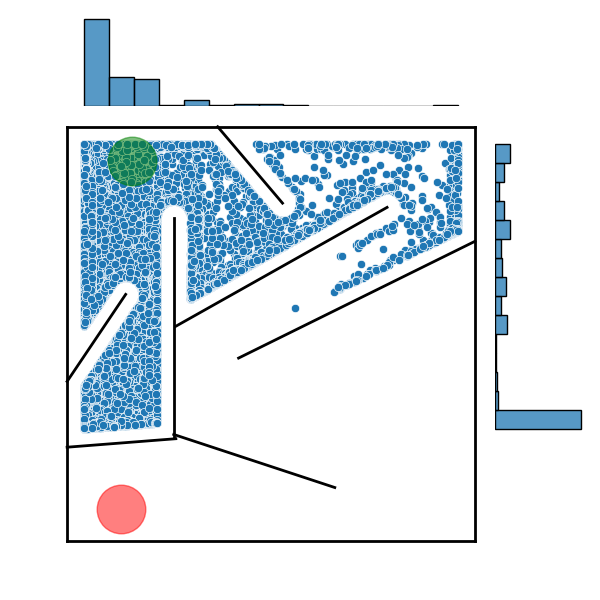
\includegraphics[scale=0.4]{resources/mazes/pure_fitness_hard_all.png}
            \caption{Fitness.}
        \end{subfigure}
        \begin{subfigure}[b]{0.5\textwidth}
            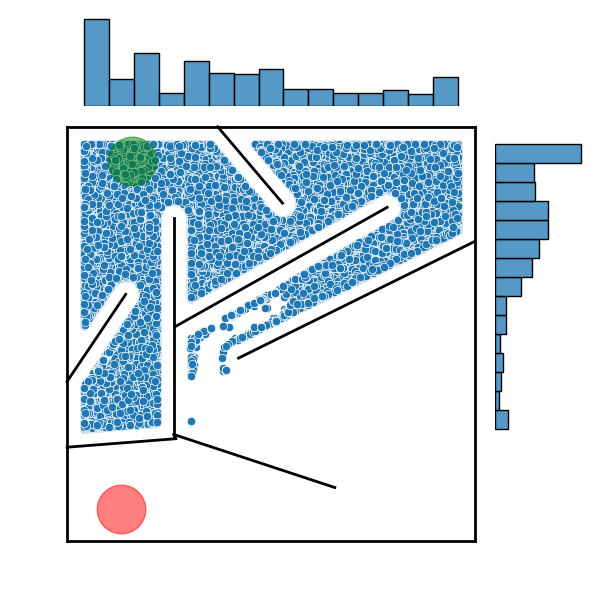
\includegraphics[scale=0.4]{resources/mazes/pure_novelty_hard_all.png}
            \caption{Novelty.}
        \end{subfigure}
        \begin{subfigure}[b]{0.5\textwidth}
            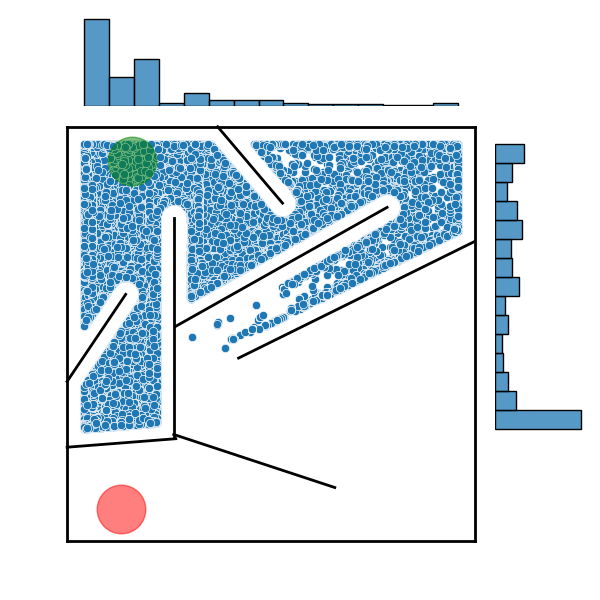
\includegraphics[scale=0.4]{resources/mazes/fitness_novelty_hard_all.png}
            \caption{LS-50.}
        \end{subfigure}
        \begin{subfigure}[b]{0.5\textwidth}
            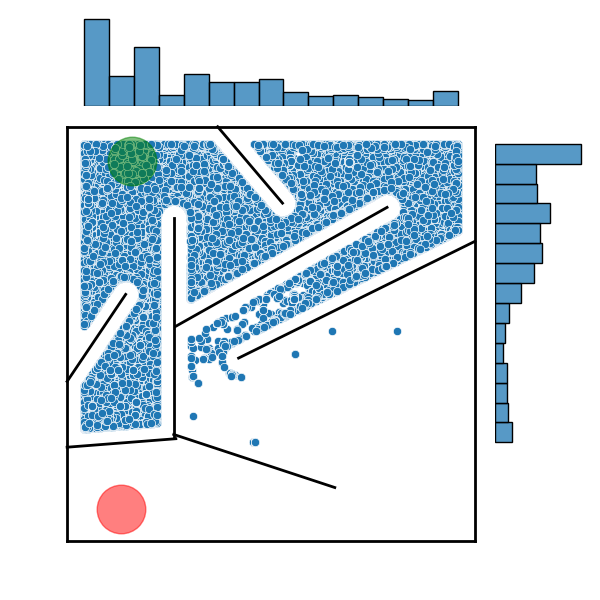
\includegraphics[scale=0.4]{resources/mazes/dynamic_hard_all.png}
            \caption{Dynamic linearisation.}
        \end{subfigure}
        \begin{subfigure}[b]{0.5\textwidth}
            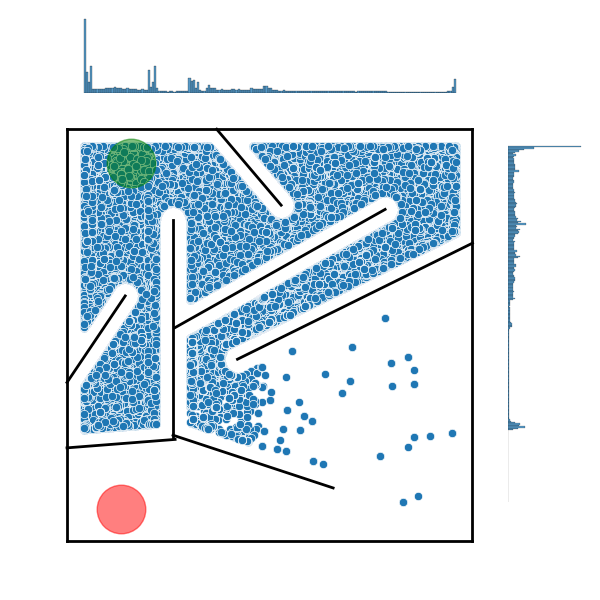
\includegraphics[scale=0.4]{resources/mazes/novelty_injection_hard_all.png}
            \caption{Novelty injection.}
        \end{subfigure}
    \end{mdframed}
    \caption{The distribution of all end-positions for each variant in the hard maze.}
    \label{distribution}
\end{figure}

\subsection{Open maze}
Only LS-50 and the dynamic combinations were able to find networks which solved the open maze, see Table \ref{open}.
\begin{table}[H]
    \centering
    \sisetup{table-format = 3.2}
    \begin{tabular}{lll}
    \toprule
    Statistic & \multicolumn{1}{l}{LS-50} & \multicolumn{1}{l}{DL} \\
    \midrule
    Successful runs & 12 & 2 \\
    Worst run (evaluations) & 122004 & 137803 \\
    \rowcolor[gray]{.9} Mean evaluations until solved & 82608 & 129205 \\
    Standard deviation & 32539  & 12159 \\
    \rowcolor[gray]{.9} Mean hidden nodes of solutions & 23.1 & 45.5 \\
    Standard deviation & 10.1 & 10.6 \\
    \rowcolor[gray]{.9} Mean links of solutions & 82.3  & 150 \\
    Standard deviation & 31.9  & 31.1 \\
    \bottomrule
    \end{tabular}
    \caption{Results for the open maze, data was collected for each variant over 30 runs.}
    \label{open}
\end{table}

\begin{figure}[H]
    \begin{center}
        %% Creator: Matplotlib, PGF backend
%%
%% To include the figure in your LaTeX document, write
%%   \input{<filename>.pgf}
%%
%% Make sure the required packages are loaded in your preamble
%%   \usepackage{pgf}
%%
%% and, on pdftex
%%   \usepackage[utf8]{inputenc}\DeclareUnicodeCharacter{2212}{-}
%%
%% or, on luatex and xetex
%%   \usepackage{unicode-math}
%%
%% Figures using additional raster images can only be included by \input if
%% they are in the same directory as the main LaTeX file. For loading figures
%% from other directories you can use the `import` package
%%   \usepackage{import}
%%
%% and then include the figures with
%%   \import{<path to file>}{<filename>.pgf}
%%
%% Matplotlib used the following preamble
%%
\begingroup%
\makeatletter%
\begin{pgfpicture}%
\pgfpathrectangle{\pgfpointorigin}{\pgfqpoint{3.854013in}{2.909691in}}%
\pgfusepath{use as bounding box, clip}%
\begin{pgfscope}%
\pgfsetbuttcap%
\pgfsetmiterjoin%
\definecolor{currentfill}{rgb}{1.000000,1.000000,1.000000}%
\pgfsetfillcolor{currentfill}%
\pgfsetlinewidth{0.000000pt}%
\definecolor{currentstroke}{rgb}{1.000000,1.000000,1.000000}%
\pgfsetstrokecolor{currentstroke}%
\pgfsetdash{}{0pt}%
\pgfpathmoveto{\pgfqpoint{0.000000in}{0.000000in}}%
\pgfpathlineto{\pgfqpoint{3.854013in}{0.000000in}}%
\pgfpathlineto{\pgfqpoint{3.854013in}{2.909691in}}%
\pgfpathlineto{\pgfqpoint{0.000000in}{2.909691in}}%
\pgfpathclose%
\pgfusepath{fill}%
\end{pgfscope}%
\begin{pgfscope}%
\pgfsetbuttcap%
\pgfsetmiterjoin%
\definecolor{currentfill}{rgb}{1.000000,1.000000,1.000000}%
\pgfsetfillcolor{currentfill}%
\pgfsetlinewidth{0.000000pt}%
\definecolor{currentstroke}{rgb}{0.000000,0.000000,0.000000}%
\pgfsetstrokecolor{currentstroke}%
\pgfsetstrokeopacity{0.000000}%
\pgfsetdash{}{0pt}%
\pgfpathmoveto{\pgfqpoint{0.654013in}{0.499691in}}%
\pgfpathlineto{\pgfqpoint{3.754013in}{0.499691in}}%
\pgfpathlineto{\pgfqpoint{3.754013in}{2.809691in}}%
\pgfpathlineto{\pgfqpoint{0.654013in}{2.809691in}}%
\pgfpathclose%
\pgfusepath{fill}%
\end{pgfscope}%
\begin{pgfscope}%
\pgfsetbuttcap%
\pgfsetroundjoin%
\definecolor{currentfill}{rgb}{0.000000,0.000000,0.000000}%
\pgfsetfillcolor{currentfill}%
\pgfsetlinewidth{0.803000pt}%
\definecolor{currentstroke}{rgb}{0.000000,0.000000,0.000000}%
\pgfsetstrokecolor{currentstroke}%
\pgfsetdash{}{0pt}%
\pgfsys@defobject{currentmarker}{\pgfqpoint{0.000000in}{-0.048611in}}{\pgfqpoint{0.000000in}{0.000000in}}{%
\pgfpathmoveto{\pgfqpoint{0.000000in}{0.000000in}}%
\pgfpathlineto{\pgfqpoint{0.000000in}{-0.048611in}}%
\pgfusepath{stroke,fill}%
}%
\begin{pgfscope}%
\pgfsys@transformshift{0.794922in}{0.499691in}%
\pgfsys@useobject{currentmarker}{}%
\end{pgfscope}%
\end{pgfscope}%
\begin{pgfscope}%
\definecolor{textcolor}{rgb}{0.000000,0.000000,0.000000}%
\pgfsetstrokecolor{textcolor}%
\pgfsetfillcolor{textcolor}%
\pgftext[x=0.794922in,y=0.402469in,,top]{\color{textcolor}\rmfamily\fontsize{10.000000}{12.000000}\selectfont \(\displaystyle {0}\)}%
\end{pgfscope}%
\begin{pgfscope}%
\pgfsetbuttcap%
\pgfsetroundjoin%
\definecolor{currentfill}{rgb}{0.000000,0.000000,0.000000}%
\pgfsetfillcolor{currentfill}%
\pgfsetlinewidth{0.803000pt}%
\definecolor{currentstroke}{rgb}{0.000000,0.000000,0.000000}%
\pgfsetstrokecolor{currentstroke}%
\pgfsetdash{}{0pt}%
\pgfsys@defobject{currentmarker}{\pgfqpoint{0.000000in}{-0.048611in}}{\pgfqpoint{0.000000in}{0.000000in}}{%
\pgfpathmoveto{\pgfqpoint{0.000000in}{0.000000in}}%
\pgfpathlineto{\pgfqpoint{0.000000in}{-0.048611in}}%
\pgfusepath{stroke,fill}%
}%
\begin{pgfscope}%
\pgfsys@transformshift{1.601269in}{0.499691in}%
\pgfsys@useobject{currentmarker}{}%
\end{pgfscope}%
\end{pgfscope}%
\begin{pgfscope}%
\definecolor{textcolor}{rgb}{0.000000,0.000000,0.000000}%
\pgfsetstrokecolor{textcolor}%
\pgfsetfillcolor{textcolor}%
\pgftext[x=1.601269in,y=0.402469in,,top]{\color{textcolor}\rmfamily\fontsize{10.000000}{12.000000}\selectfont \(\displaystyle {200}\)}%
\end{pgfscope}%
\begin{pgfscope}%
\pgfsetbuttcap%
\pgfsetroundjoin%
\definecolor{currentfill}{rgb}{0.000000,0.000000,0.000000}%
\pgfsetfillcolor{currentfill}%
\pgfsetlinewidth{0.803000pt}%
\definecolor{currentstroke}{rgb}{0.000000,0.000000,0.000000}%
\pgfsetstrokecolor{currentstroke}%
\pgfsetdash{}{0pt}%
\pgfsys@defobject{currentmarker}{\pgfqpoint{0.000000in}{-0.048611in}}{\pgfqpoint{0.000000in}{0.000000in}}{%
\pgfpathmoveto{\pgfqpoint{0.000000in}{0.000000in}}%
\pgfpathlineto{\pgfqpoint{0.000000in}{-0.048611in}}%
\pgfusepath{stroke,fill}%
}%
\begin{pgfscope}%
\pgfsys@transformshift{2.407616in}{0.499691in}%
\pgfsys@useobject{currentmarker}{}%
\end{pgfscope}%
\end{pgfscope}%
\begin{pgfscope}%
\definecolor{textcolor}{rgb}{0.000000,0.000000,0.000000}%
\pgfsetstrokecolor{textcolor}%
\pgfsetfillcolor{textcolor}%
\pgftext[x=2.407616in,y=0.402469in,,top]{\color{textcolor}\rmfamily\fontsize{10.000000}{12.000000}\selectfont \(\displaystyle {400}\)}%
\end{pgfscope}%
\begin{pgfscope}%
\pgfsetbuttcap%
\pgfsetroundjoin%
\definecolor{currentfill}{rgb}{0.000000,0.000000,0.000000}%
\pgfsetfillcolor{currentfill}%
\pgfsetlinewidth{0.803000pt}%
\definecolor{currentstroke}{rgb}{0.000000,0.000000,0.000000}%
\pgfsetstrokecolor{currentstroke}%
\pgfsetdash{}{0pt}%
\pgfsys@defobject{currentmarker}{\pgfqpoint{0.000000in}{-0.048611in}}{\pgfqpoint{0.000000in}{0.000000in}}{%
\pgfpathmoveto{\pgfqpoint{0.000000in}{0.000000in}}%
\pgfpathlineto{\pgfqpoint{0.000000in}{-0.048611in}}%
\pgfusepath{stroke,fill}%
}%
\begin{pgfscope}%
\pgfsys@transformshift{3.213962in}{0.499691in}%
\pgfsys@useobject{currentmarker}{}%
\end{pgfscope}%
\end{pgfscope}%
\begin{pgfscope}%
\definecolor{textcolor}{rgb}{0.000000,0.000000,0.000000}%
\pgfsetstrokecolor{textcolor}%
\pgfsetfillcolor{textcolor}%
\pgftext[x=3.213962in,y=0.402469in,,top]{\color{textcolor}\rmfamily\fontsize{10.000000}{12.000000}\selectfont \(\displaystyle {600}\)}%
\end{pgfscope}%
\begin{pgfscope}%
\definecolor{textcolor}{rgb}{0.000000,0.000000,0.000000}%
\pgfsetstrokecolor{textcolor}%
\pgfsetfillcolor{textcolor}%
\pgftext[x=2.204013in,y=0.223457in,,top]{\color{textcolor}\rmfamily\fontsize{10.000000}{12.000000}\selectfont Generations}%
\end{pgfscope}%
\begin{pgfscope}%
\pgfsetbuttcap%
\pgfsetroundjoin%
\definecolor{currentfill}{rgb}{0.000000,0.000000,0.000000}%
\pgfsetfillcolor{currentfill}%
\pgfsetlinewidth{0.803000pt}%
\definecolor{currentstroke}{rgb}{0.000000,0.000000,0.000000}%
\pgfsetstrokecolor{currentstroke}%
\pgfsetdash{}{0pt}%
\pgfsys@defobject{currentmarker}{\pgfqpoint{-0.048611in}{0.000000in}}{\pgfqpoint{-0.000000in}{0.000000in}}{%
\pgfpathmoveto{\pgfqpoint{-0.000000in}{0.000000in}}%
\pgfpathlineto{\pgfqpoint{-0.048611in}{0.000000in}}%
\pgfusepath{stroke,fill}%
}%
\begin{pgfscope}%
\pgfsys@transformshift{0.654013in}{0.588094in}%
\pgfsys@useobject{currentmarker}{}%
\end{pgfscope}%
\end{pgfscope}%
\begin{pgfscope}%
\definecolor{textcolor}{rgb}{0.000000,0.000000,0.000000}%
\pgfsetstrokecolor{textcolor}%
\pgfsetfillcolor{textcolor}%
\pgftext[x=0.279012in, y=0.539869in, left, base]{\color{textcolor}\rmfamily\fontsize{10.000000}{12.000000}\selectfont \(\displaystyle {4400}\)}%
\end{pgfscope}%
\begin{pgfscope}%
\pgfsetbuttcap%
\pgfsetroundjoin%
\definecolor{currentfill}{rgb}{0.000000,0.000000,0.000000}%
\pgfsetfillcolor{currentfill}%
\pgfsetlinewidth{0.803000pt}%
\definecolor{currentstroke}{rgb}{0.000000,0.000000,0.000000}%
\pgfsetstrokecolor{currentstroke}%
\pgfsetdash{}{0pt}%
\pgfsys@defobject{currentmarker}{\pgfqpoint{-0.048611in}{0.000000in}}{\pgfqpoint{-0.000000in}{0.000000in}}{%
\pgfpathmoveto{\pgfqpoint{-0.000000in}{0.000000in}}%
\pgfpathlineto{\pgfqpoint{-0.048611in}{0.000000in}}%
\pgfusepath{stroke,fill}%
}%
\begin{pgfscope}%
\pgfsys@transformshift{0.654013in}{1.009275in}%
\pgfsys@useobject{currentmarker}{}%
\end{pgfscope}%
\end{pgfscope}%
\begin{pgfscope}%
\definecolor{textcolor}{rgb}{0.000000,0.000000,0.000000}%
\pgfsetstrokecolor{textcolor}%
\pgfsetfillcolor{textcolor}%
\pgftext[x=0.279012in, y=0.961050in, left, base]{\color{textcolor}\rmfamily\fontsize{10.000000}{12.000000}\selectfont \(\displaystyle {4500}\)}%
\end{pgfscope}%
\begin{pgfscope}%
\pgfsetbuttcap%
\pgfsetroundjoin%
\definecolor{currentfill}{rgb}{0.000000,0.000000,0.000000}%
\pgfsetfillcolor{currentfill}%
\pgfsetlinewidth{0.803000pt}%
\definecolor{currentstroke}{rgb}{0.000000,0.000000,0.000000}%
\pgfsetstrokecolor{currentstroke}%
\pgfsetdash{}{0pt}%
\pgfsys@defobject{currentmarker}{\pgfqpoint{-0.048611in}{0.000000in}}{\pgfqpoint{-0.000000in}{0.000000in}}{%
\pgfpathmoveto{\pgfqpoint{-0.000000in}{0.000000in}}%
\pgfpathlineto{\pgfqpoint{-0.048611in}{0.000000in}}%
\pgfusepath{stroke,fill}%
}%
\begin{pgfscope}%
\pgfsys@transformshift{0.654013in}{1.430455in}%
\pgfsys@useobject{currentmarker}{}%
\end{pgfscope}%
\end{pgfscope}%
\begin{pgfscope}%
\definecolor{textcolor}{rgb}{0.000000,0.000000,0.000000}%
\pgfsetstrokecolor{textcolor}%
\pgfsetfillcolor{textcolor}%
\pgftext[x=0.279012in, y=1.382230in, left, base]{\color{textcolor}\rmfamily\fontsize{10.000000}{12.000000}\selectfont \(\displaystyle {4600}\)}%
\end{pgfscope}%
\begin{pgfscope}%
\pgfsetbuttcap%
\pgfsetroundjoin%
\definecolor{currentfill}{rgb}{0.000000,0.000000,0.000000}%
\pgfsetfillcolor{currentfill}%
\pgfsetlinewidth{0.803000pt}%
\definecolor{currentstroke}{rgb}{0.000000,0.000000,0.000000}%
\pgfsetstrokecolor{currentstroke}%
\pgfsetdash{}{0pt}%
\pgfsys@defobject{currentmarker}{\pgfqpoint{-0.048611in}{0.000000in}}{\pgfqpoint{-0.000000in}{0.000000in}}{%
\pgfpathmoveto{\pgfqpoint{-0.000000in}{0.000000in}}%
\pgfpathlineto{\pgfqpoint{-0.048611in}{0.000000in}}%
\pgfusepath{stroke,fill}%
}%
\begin{pgfscope}%
\pgfsys@transformshift{0.654013in}{1.851636in}%
\pgfsys@useobject{currentmarker}{}%
\end{pgfscope}%
\end{pgfscope}%
\begin{pgfscope}%
\definecolor{textcolor}{rgb}{0.000000,0.000000,0.000000}%
\pgfsetstrokecolor{textcolor}%
\pgfsetfillcolor{textcolor}%
\pgftext[x=0.279012in, y=1.803410in, left, base]{\color{textcolor}\rmfamily\fontsize{10.000000}{12.000000}\selectfont \(\displaystyle {4700}\)}%
\end{pgfscope}%
\begin{pgfscope}%
\pgfsetbuttcap%
\pgfsetroundjoin%
\definecolor{currentfill}{rgb}{0.000000,0.000000,0.000000}%
\pgfsetfillcolor{currentfill}%
\pgfsetlinewidth{0.803000pt}%
\definecolor{currentstroke}{rgb}{0.000000,0.000000,0.000000}%
\pgfsetstrokecolor{currentstroke}%
\pgfsetdash{}{0pt}%
\pgfsys@defobject{currentmarker}{\pgfqpoint{-0.048611in}{0.000000in}}{\pgfqpoint{-0.000000in}{0.000000in}}{%
\pgfpathmoveto{\pgfqpoint{-0.000000in}{0.000000in}}%
\pgfpathlineto{\pgfqpoint{-0.048611in}{0.000000in}}%
\pgfusepath{stroke,fill}%
}%
\begin{pgfscope}%
\pgfsys@transformshift{0.654013in}{2.272816in}%
\pgfsys@useobject{currentmarker}{}%
\end{pgfscope}%
\end{pgfscope}%
\begin{pgfscope}%
\definecolor{textcolor}{rgb}{0.000000,0.000000,0.000000}%
\pgfsetstrokecolor{textcolor}%
\pgfsetfillcolor{textcolor}%
\pgftext[x=0.279012in, y=2.224591in, left, base]{\color{textcolor}\rmfamily\fontsize{10.000000}{12.000000}\selectfont \(\displaystyle {4800}\)}%
\end{pgfscope}%
\begin{pgfscope}%
\pgfsetbuttcap%
\pgfsetroundjoin%
\definecolor{currentfill}{rgb}{0.000000,0.000000,0.000000}%
\pgfsetfillcolor{currentfill}%
\pgfsetlinewidth{0.803000pt}%
\definecolor{currentstroke}{rgb}{0.000000,0.000000,0.000000}%
\pgfsetstrokecolor{currentstroke}%
\pgfsetdash{}{0pt}%
\pgfsys@defobject{currentmarker}{\pgfqpoint{-0.048611in}{0.000000in}}{\pgfqpoint{-0.000000in}{0.000000in}}{%
\pgfpathmoveto{\pgfqpoint{-0.000000in}{0.000000in}}%
\pgfpathlineto{\pgfqpoint{-0.048611in}{0.000000in}}%
\pgfusepath{stroke,fill}%
}%
\begin{pgfscope}%
\pgfsys@transformshift{0.654013in}{2.693996in}%
\pgfsys@useobject{currentmarker}{}%
\end{pgfscope}%
\end{pgfscope}%
\begin{pgfscope}%
\definecolor{textcolor}{rgb}{0.000000,0.000000,0.000000}%
\pgfsetstrokecolor{textcolor}%
\pgfsetfillcolor{textcolor}%
\pgftext[x=0.279012in, y=2.645771in, left, base]{\color{textcolor}\rmfamily\fontsize{10.000000}{12.000000}\selectfont \(\displaystyle {4900}\)}%
\end{pgfscope}%
\begin{pgfscope}%
\definecolor{textcolor}{rgb}{0.000000,0.000000,0.000000}%
\pgfsetstrokecolor{textcolor}%
\pgfsetfillcolor{textcolor}%
\pgftext[x=0.223457in,y=1.654691in,,bottom,rotate=90.000000]{\color{textcolor}\rmfamily\fontsize{10.000000}{12.000000}\selectfont Average fitness}%
\end{pgfscope}%
\begin{pgfscope}%
\pgfpathrectangle{\pgfqpoint{0.654013in}{0.499691in}}{\pgfqpoint{3.100000in}{2.310000in}}%
\pgfusepath{clip}%
\pgfsetrectcap%
\pgfsetroundjoin%
\pgfsetlinewidth{1.505625pt}%
\definecolor{currentstroke}{rgb}{0.121569,0.466667,0.705882}%
\pgfsetstrokecolor{currentstroke}%
\pgfsetdash{}{0pt}%
\pgfpathmoveto{\pgfqpoint{0.794922in}{2.101735in}}%
\pgfpathlineto{\pgfqpoint{0.798954in}{2.260172in}}%
\pgfpathlineto{\pgfqpoint{0.802986in}{2.346294in}}%
\pgfpathlineto{\pgfqpoint{0.807017in}{2.370912in}}%
\pgfpathlineto{\pgfqpoint{0.819113in}{2.506503in}}%
\pgfpathlineto{\pgfqpoint{0.823144in}{2.515492in}}%
\pgfpathlineto{\pgfqpoint{0.827176in}{2.530094in}}%
\pgfpathlineto{\pgfqpoint{0.831208in}{2.558277in}}%
\pgfpathlineto{\pgfqpoint{0.835239in}{2.553075in}}%
\pgfpathlineto{\pgfqpoint{0.839271in}{2.571056in}}%
\pgfpathlineto{\pgfqpoint{0.843303in}{2.574566in}}%
\pgfpathlineto{\pgfqpoint{0.847335in}{2.588707in}}%
\pgfpathlineto{\pgfqpoint{0.851366in}{2.583999in}}%
\pgfpathlineto{\pgfqpoint{0.855398in}{2.595689in}}%
\pgfpathlineto{\pgfqpoint{0.859430in}{2.594239in}}%
\pgfpathlineto{\pgfqpoint{0.863462in}{2.605189in}}%
\pgfpathlineto{\pgfqpoint{0.867493in}{2.600121in}}%
\pgfpathlineto{\pgfqpoint{0.871525in}{2.601021in}}%
\pgfpathlineto{\pgfqpoint{0.875557in}{2.613548in}}%
\pgfpathlineto{\pgfqpoint{0.883620in}{2.618772in}}%
\pgfpathlineto{\pgfqpoint{0.887652in}{2.625152in}}%
\pgfpathlineto{\pgfqpoint{0.891684in}{2.622285in}}%
\pgfpathlineto{\pgfqpoint{0.895715in}{2.603328in}}%
\pgfpathlineto{\pgfqpoint{0.899747in}{2.622765in}}%
\pgfpathlineto{\pgfqpoint{0.903779in}{2.604996in}}%
\pgfpathlineto{\pgfqpoint{0.911842in}{2.628449in}}%
\pgfpathlineto{\pgfqpoint{0.915874in}{2.625576in}}%
\pgfpathlineto{\pgfqpoint{0.919906in}{2.624335in}}%
\pgfpathlineto{\pgfqpoint{0.923938in}{2.625890in}}%
\pgfpathlineto{\pgfqpoint{0.927969in}{2.629785in}}%
\pgfpathlineto{\pgfqpoint{0.932001in}{2.617646in}}%
\pgfpathlineto{\pgfqpoint{0.936033in}{2.621038in}}%
\pgfpathlineto{\pgfqpoint{0.940065in}{2.636489in}}%
\pgfpathlineto{\pgfqpoint{0.948128in}{2.625036in}}%
\pgfpathlineto{\pgfqpoint{0.952160in}{2.633204in}}%
\pgfpathlineto{\pgfqpoint{0.956191in}{2.621506in}}%
\pgfpathlineto{\pgfqpoint{0.964255in}{2.641823in}}%
\pgfpathlineto{\pgfqpoint{0.968287in}{2.631956in}}%
\pgfpathlineto{\pgfqpoint{0.972318in}{2.652835in}}%
\pgfpathlineto{\pgfqpoint{0.976350in}{2.640272in}}%
\pgfpathlineto{\pgfqpoint{0.980382in}{2.651233in}}%
\pgfpathlineto{\pgfqpoint{0.984414in}{2.640469in}}%
\pgfpathlineto{\pgfqpoint{0.988445in}{2.645477in}}%
\pgfpathlineto{\pgfqpoint{0.992477in}{2.638741in}}%
\pgfpathlineto{\pgfqpoint{0.996509in}{2.647551in}}%
\pgfpathlineto{\pgfqpoint{1.000541in}{2.636802in}}%
\pgfpathlineto{\pgfqpoint{1.004572in}{2.648418in}}%
\pgfpathlineto{\pgfqpoint{1.012636in}{2.643238in}}%
\pgfpathlineto{\pgfqpoint{1.016667in}{2.647712in}}%
\pgfpathlineto{\pgfqpoint{1.020699in}{2.648418in}}%
\pgfpathlineto{\pgfqpoint{1.024731in}{2.643320in}}%
\pgfpathlineto{\pgfqpoint{1.028763in}{2.656850in}}%
\pgfpathlineto{\pgfqpoint{1.032794in}{2.654868in}}%
\pgfpathlineto{\pgfqpoint{1.036826in}{2.640239in}}%
\pgfpathlineto{\pgfqpoint{1.040858in}{2.649594in}}%
\pgfpathlineto{\pgfqpoint{1.044890in}{2.668452in}}%
\pgfpathlineto{\pgfqpoint{1.048921in}{2.642799in}}%
\pgfpathlineto{\pgfqpoint{1.052953in}{2.643245in}}%
\pgfpathlineto{\pgfqpoint{1.056985in}{2.658849in}}%
\pgfpathlineto{\pgfqpoint{1.061017in}{2.645205in}}%
\pgfpathlineto{\pgfqpoint{1.065048in}{2.653565in}}%
\pgfpathlineto{\pgfqpoint{1.069080in}{2.645625in}}%
\pgfpathlineto{\pgfqpoint{1.073112in}{2.665016in}}%
\pgfpathlineto{\pgfqpoint{1.077144in}{2.649604in}}%
\pgfpathlineto{\pgfqpoint{1.081175in}{2.656706in}}%
\pgfpathlineto{\pgfqpoint{1.085207in}{2.649859in}}%
\pgfpathlineto{\pgfqpoint{1.089239in}{2.657388in}}%
\pgfpathlineto{\pgfqpoint{1.093270in}{2.652508in}}%
\pgfpathlineto{\pgfqpoint{1.097302in}{2.667876in}}%
\pgfpathlineto{\pgfqpoint{1.101334in}{2.659437in}}%
\pgfpathlineto{\pgfqpoint{1.105366in}{2.664400in}}%
\pgfpathlineto{\pgfqpoint{1.109397in}{2.662994in}}%
\pgfpathlineto{\pgfqpoint{1.113429in}{2.650151in}}%
\pgfpathlineto{\pgfqpoint{1.117461in}{2.669166in}}%
\pgfpathlineto{\pgfqpoint{1.121493in}{2.654789in}}%
\pgfpathlineto{\pgfqpoint{1.125524in}{2.667935in}}%
\pgfpathlineto{\pgfqpoint{1.129556in}{2.673963in}}%
\pgfpathlineto{\pgfqpoint{1.133588in}{2.677381in}}%
\pgfpathlineto{\pgfqpoint{1.137620in}{2.664901in}}%
\pgfpathlineto{\pgfqpoint{1.145683in}{2.656726in}}%
\pgfpathlineto{\pgfqpoint{1.149715in}{2.678621in}}%
\pgfpathlineto{\pgfqpoint{1.153746in}{2.663157in}}%
\pgfpathlineto{\pgfqpoint{1.157778in}{2.664417in}}%
\pgfpathlineto{\pgfqpoint{1.161810in}{2.668027in}}%
\pgfpathlineto{\pgfqpoint{1.169873in}{2.653225in}}%
\pgfpathlineto{\pgfqpoint{1.177937in}{2.660901in}}%
\pgfpathlineto{\pgfqpoint{1.181969in}{2.651180in}}%
\pgfpathlineto{\pgfqpoint{1.190032in}{2.673419in}}%
\pgfpathlineto{\pgfqpoint{1.194064in}{2.661588in}}%
\pgfpathlineto{\pgfqpoint{1.198096in}{2.661042in}}%
\pgfpathlineto{\pgfqpoint{1.202127in}{2.670012in}}%
\pgfpathlineto{\pgfqpoint{1.206159in}{2.657397in}}%
\pgfpathlineto{\pgfqpoint{1.210191in}{2.670349in}}%
\pgfpathlineto{\pgfqpoint{1.214222in}{2.666828in}}%
\pgfpathlineto{\pgfqpoint{1.222286in}{2.666157in}}%
\pgfpathlineto{\pgfqpoint{1.226318in}{2.673500in}}%
\pgfpathlineto{\pgfqpoint{1.230349in}{2.670172in}}%
\pgfpathlineto{\pgfqpoint{1.234381in}{2.670167in}}%
\pgfpathlineto{\pgfqpoint{1.238413in}{2.660742in}}%
\pgfpathlineto{\pgfqpoint{1.242445in}{2.661294in}}%
\pgfpathlineto{\pgfqpoint{1.246476in}{2.670180in}}%
\pgfpathlineto{\pgfqpoint{1.254540in}{2.656368in}}%
\pgfpathlineto{\pgfqpoint{1.258572in}{2.666887in}}%
\pgfpathlineto{\pgfqpoint{1.262603in}{2.663833in}}%
\pgfpathlineto{\pgfqpoint{1.266635in}{2.665350in}}%
\pgfpathlineto{\pgfqpoint{1.274698in}{2.661048in}}%
\pgfpathlineto{\pgfqpoint{1.278730in}{2.662880in}}%
\pgfpathlineto{\pgfqpoint{1.282762in}{2.669510in}}%
\pgfpathlineto{\pgfqpoint{1.286794in}{2.665522in}}%
\pgfpathlineto{\pgfqpoint{1.290825in}{2.668210in}}%
\pgfpathlineto{\pgfqpoint{1.294857in}{2.679701in}}%
\pgfpathlineto{\pgfqpoint{1.298889in}{2.665545in}}%
\pgfpathlineto{\pgfqpoint{1.302921in}{2.673614in}}%
\pgfpathlineto{\pgfqpoint{1.306952in}{2.668869in}}%
\pgfpathlineto{\pgfqpoint{1.310984in}{2.674811in}}%
\pgfpathlineto{\pgfqpoint{1.315016in}{2.670444in}}%
\pgfpathlineto{\pgfqpoint{1.319048in}{2.663428in}}%
\pgfpathlineto{\pgfqpoint{1.323079in}{2.665960in}}%
\pgfpathlineto{\pgfqpoint{1.331143in}{2.676307in}}%
\pgfpathlineto{\pgfqpoint{1.335174in}{2.665584in}}%
\pgfpathlineto{\pgfqpoint{1.339206in}{2.664645in}}%
\pgfpathlineto{\pgfqpoint{1.343238in}{2.680689in}}%
\pgfpathlineto{\pgfqpoint{1.347270in}{2.664505in}}%
\pgfpathlineto{\pgfqpoint{1.351301in}{2.664332in}}%
\pgfpathlineto{\pgfqpoint{1.355333in}{2.678480in}}%
\pgfpathlineto{\pgfqpoint{1.359365in}{2.669399in}}%
\pgfpathlineto{\pgfqpoint{1.363397in}{2.678755in}}%
\pgfpathlineto{\pgfqpoint{1.367428in}{2.682741in}}%
\pgfpathlineto{\pgfqpoint{1.371460in}{2.671481in}}%
\pgfpathlineto{\pgfqpoint{1.375492in}{2.686238in}}%
\pgfpathlineto{\pgfqpoint{1.379524in}{2.673385in}}%
\pgfpathlineto{\pgfqpoint{1.383555in}{2.669195in}}%
\pgfpathlineto{\pgfqpoint{1.387587in}{2.683544in}}%
\pgfpathlineto{\pgfqpoint{1.391619in}{2.678786in}}%
\pgfpathlineto{\pgfqpoint{1.395650in}{2.668058in}}%
\pgfpathlineto{\pgfqpoint{1.399682in}{2.667572in}}%
\pgfpathlineto{\pgfqpoint{1.403714in}{2.678686in}}%
\pgfpathlineto{\pgfqpoint{1.407746in}{2.673393in}}%
\pgfpathlineto{\pgfqpoint{1.411777in}{2.676190in}}%
\pgfpathlineto{\pgfqpoint{1.415809in}{2.676930in}}%
\pgfpathlineto{\pgfqpoint{1.419841in}{2.682855in}}%
\pgfpathlineto{\pgfqpoint{1.423873in}{2.675328in}}%
\pgfpathlineto{\pgfqpoint{1.427904in}{2.671262in}}%
\pgfpathlineto{\pgfqpoint{1.431936in}{2.680905in}}%
\pgfpathlineto{\pgfqpoint{1.435968in}{2.670897in}}%
\pgfpathlineto{\pgfqpoint{1.440000in}{2.675467in}}%
\pgfpathlineto{\pgfqpoint{1.444031in}{2.671549in}}%
\pgfpathlineto{\pgfqpoint{1.448063in}{2.682044in}}%
\pgfpathlineto{\pgfqpoint{1.452095in}{2.674792in}}%
\pgfpathlineto{\pgfqpoint{1.456126in}{2.670643in}}%
\pgfpathlineto{\pgfqpoint{1.460158in}{2.682162in}}%
\pgfpathlineto{\pgfqpoint{1.464190in}{2.678485in}}%
\pgfpathlineto{\pgfqpoint{1.468222in}{2.682799in}}%
\pgfpathlineto{\pgfqpoint{1.472253in}{2.691622in}}%
\pgfpathlineto{\pgfqpoint{1.476285in}{2.675951in}}%
\pgfpathlineto{\pgfqpoint{1.484349in}{2.684762in}}%
\pgfpathlineto{\pgfqpoint{1.488380in}{2.680527in}}%
\pgfpathlineto{\pgfqpoint{1.492412in}{2.683812in}}%
\pgfpathlineto{\pgfqpoint{1.496444in}{2.682638in}}%
\pgfpathlineto{\pgfqpoint{1.500476in}{2.684537in}}%
\pgfpathlineto{\pgfqpoint{1.504507in}{2.684404in}}%
\pgfpathlineto{\pgfqpoint{1.508539in}{2.681072in}}%
\pgfpathlineto{\pgfqpoint{1.512571in}{2.690774in}}%
\pgfpathlineto{\pgfqpoint{1.516602in}{2.684487in}}%
\pgfpathlineto{\pgfqpoint{1.520634in}{2.682614in}}%
\pgfpathlineto{\pgfqpoint{1.524666in}{2.679097in}}%
\pgfpathlineto{\pgfqpoint{1.528698in}{2.688557in}}%
\pgfpathlineto{\pgfqpoint{1.532729in}{2.684636in}}%
\pgfpathlineto{\pgfqpoint{1.536761in}{2.686747in}}%
\pgfpathlineto{\pgfqpoint{1.540793in}{2.696172in}}%
\pgfpathlineto{\pgfqpoint{1.544825in}{2.682237in}}%
\pgfpathlineto{\pgfqpoint{1.548856in}{2.685247in}}%
\pgfpathlineto{\pgfqpoint{1.552888in}{2.672327in}}%
\pgfpathlineto{\pgfqpoint{1.556920in}{2.685606in}}%
\pgfpathlineto{\pgfqpoint{1.560952in}{2.687647in}}%
\pgfpathlineto{\pgfqpoint{1.564983in}{2.677139in}}%
\pgfpathlineto{\pgfqpoint{1.577078in}{2.683113in}}%
\pgfpathlineto{\pgfqpoint{1.581110in}{2.679251in}}%
\pgfpathlineto{\pgfqpoint{1.585142in}{2.688103in}}%
\pgfpathlineto{\pgfqpoint{1.589174in}{2.693186in}}%
\pgfpathlineto{\pgfqpoint{1.601269in}{2.672222in}}%
\pgfpathlineto{\pgfqpoint{1.605301in}{2.679999in}}%
\pgfpathlineto{\pgfqpoint{1.609332in}{2.690389in}}%
\pgfpathlineto{\pgfqpoint{1.613364in}{2.690773in}}%
\pgfpathlineto{\pgfqpoint{1.617396in}{2.688243in}}%
\pgfpathlineto{\pgfqpoint{1.621428in}{2.675688in}}%
\pgfpathlineto{\pgfqpoint{1.625459in}{2.683449in}}%
\pgfpathlineto{\pgfqpoint{1.629491in}{2.684313in}}%
\pgfpathlineto{\pgfqpoint{1.633523in}{2.686352in}}%
\pgfpathlineto{\pgfqpoint{1.637554in}{2.691773in}}%
\pgfpathlineto{\pgfqpoint{1.641586in}{2.688030in}}%
\pgfpathlineto{\pgfqpoint{1.645618in}{2.692062in}}%
\pgfpathlineto{\pgfqpoint{1.649650in}{2.692767in}}%
\pgfpathlineto{\pgfqpoint{1.653681in}{2.689716in}}%
\pgfpathlineto{\pgfqpoint{1.657713in}{2.681947in}}%
\pgfpathlineto{\pgfqpoint{1.661745in}{2.692186in}}%
\pgfpathlineto{\pgfqpoint{1.665777in}{2.694166in}}%
\pgfpathlineto{\pgfqpoint{1.669808in}{2.693477in}}%
\pgfpathlineto{\pgfqpoint{1.677872in}{2.695303in}}%
\pgfpathlineto{\pgfqpoint{1.681904in}{2.688514in}}%
\pgfpathlineto{\pgfqpoint{1.685935in}{2.673266in}}%
\pgfpathlineto{\pgfqpoint{1.689967in}{2.693249in}}%
\pgfpathlineto{\pgfqpoint{1.693999in}{2.699912in}}%
\pgfpathlineto{\pgfqpoint{1.698030in}{2.690754in}}%
\pgfpathlineto{\pgfqpoint{1.702062in}{2.688690in}}%
\pgfpathlineto{\pgfqpoint{1.706094in}{2.682244in}}%
\pgfpathlineto{\pgfqpoint{1.710126in}{2.693072in}}%
\pgfpathlineto{\pgfqpoint{1.714157in}{2.697751in}}%
\pgfpathlineto{\pgfqpoint{1.718189in}{2.694794in}}%
\pgfpathlineto{\pgfqpoint{1.722221in}{2.683573in}}%
\pgfpathlineto{\pgfqpoint{1.726253in}{2.690077in}}%
\pgfpathlineto{\pgfqpoint{1.730284in}{2.688560in}}%
\pgfpathlineto{\pgfqpoint{1.734316in}{2.693261in}}%
\pgfpathlineto{\pgfqpoint{1.738348in}{2.679889in}}%
\pgfpathlineto{\pgfqpoint{1.742380in}{2.683963in}}%
\pgfpathlineto{\pgfqpoint{1.746411in}{2.679186in}}%
\pgfpathlineto{\pgfqpoint{1.750443in}{2.683571in}}%
\pgfpathlineto{\pgfqpoint{1.754475in}{2.679359in}}%
\pgfpathlineto{\pgfqpoint{1.758506in}{2.679259in}}%
\pgfpathlineto{\pgfqpoint{1.766570in}{2.689572in}}%
\pgfpathlineto{\pgfqpoint{1.770602in}{2.690812in}}%
\pgfpathlineto{\pgfqpoint{1.774633in}{2.698076in}}%
\pgfpathlineto{\pgfqpoint{1.778665in}{2.696320in}}%
\pgfpathlineto{\pgfqpoint{1.782697in}{2.690747in}}%
\pgfpathlineto{\pgfqpoint{1.786729in}{2.677730in}}%
\pgfpathlineto{\pgfqpoint{1.790760in}{2.683428in}}%
\pgfpathlineto{\pgfqpoint{1.794792in}{2.683174in}}%
\pgfpathlineto{\pgfqpoint{1.798824in}{2.692735in}}%
\pgfpathlineto{\pgfqpoint{1.802856in}{2.685154in}}%
\pgfpathlineto{\pgfqpoint{1.810919in}{2.684692in}}%
\pgfpathlineto{\pgfqpoint{1.814951in}{2.687654in}}%
\pgfpathlineto{\pgfqpoint{1.818982in}{2.679683in}}%
\pgfpathlineto{\pgfqpoint{1.823014in}{2.694992in}}%
\pgfpathlineto{\pgfqpoint{1.827046in}{2.689007in}}%
\pgfpathlineto{\pgfqpoint{1.831078in}{2.687925in}}%
\pgfpathlineto{\pgfqpoint{1.835109in}{2.685122in}}%
\pgfpathlineto{\pgfqpoint{1.839141in}{2.688557in}}%
\pgfpathlineto{\pgfqpoint{1.851236in}{2.678426in}}%
\pgfpathlineto{\pgfqpoint{1.855268in}{2.673422in}}%
\pgfpathlineto{\pgfqpoint{1.859300in}{2.689460in}}%
\pgfpathlineto{\pgfqpoint{1.863332in}{2.680140in}}%
\pgfpathlineto{\pgfqpoint{1.867363in}{2.680582in}}%
\pgfpathlineto{\pgfqpoint{1.879458in}{2.687376in}}%
\pgfpathlineto{\pgfqpoint{1.887522in}{2.699269in}}%
\pgfpathlineto{\pgfqpoint{1.891554in}{2.693898in}}%
\pgfpathlineto{\pgfqpoint{1.895585in}{2.693295in}}%
\pgfpathlineto{\pgfqpoint{1.899617in}{2.685227in}}%
\pgfpathlineto{\pgfqpoint{1.903649in}{2.679686in}}%
\pgfpathlineto{\pgfqpoint{1.907681in}{2.693135in}}%
\pgfpathlineto{\pgfqpoint{1.911712in}{2.678536in}}%
\pgfpathlineto{\pgfqpoint{1.915744in}{2.686192in}}%
\pgfpathlineto{\pgfqpoint{1.919776in}{2.678667in}}%
\pgfpathlineto{\pgfqpoint{1.923808in}{2.696712in}}%
\pgfpathlineto{\pgfqpoint{1.927839in}{2.688131in}}%
\pgfpathlineto{\pgfqpoint{1.935903in}{2.686654in}}%
\pgfpathlineto{\pgfqpoint{1.939935in}{2.681247in}}%
\pgfpathlineto{\pgfqpoint{1.943966in}{2.683287in}}%
\pgfpathlineto{\pgfqpoint{1.947998in}{2.690823in}}%
\pgfpathlineto{\pgfqpoint{1.952030in}{2.686497in}}%
\pgfpathlineto{\pgfqpoint{1.960093in}{2.697644in}}%
\pgfpathlineto{\pgfqpoint{1.964125in}{2.683299in}}%
\pgfpathlineto{\pgfqpoint{1.968157in}{2.686688in}}%
\pgfpathlineto{\pgfqpoint{1.972188in}{2.682967in}}%
\pgfpathlineto{\pgfqpoint{1.976220in}{2.696746in}}%
\pgfpathlineto{\pgfqpoint{1.980252in}{2.695681in}}%
\pgfpathlineto{\pgfqpoint{1.984284in}{2.698539in}}%
\pgfpathlineto{\pgfqpoint{1.988315in}{2.692495in}}%
\pgfpathlineto{\pgfqpoint{1.992347in}{2.677426in}}%
\pgfpathlineto{\pgfqpoint{1.996379in}{2.688174in}}%
\pgfpathlineto{\pgfqpoint{2.000411in}{2.684982in}}%
\pgfpathlineto{\pgfqpoint{2.004442in}{2.694126in}}%
\pgfpathlineto{\pgfqpoint{2.008474in}{2.693559in}}%
\pgfpathlineto{\pgfqpoint{2.012506in}{2.699552in}}%
\pgfpathlineto{\pgfqpoint{2.016537in}{2.688907in}}%
\pgfpathlineto{\pgfqpoint{2.020569in}{2.698200in}}%
\pgfpathlineto{\pgfqpoint{2.024601in}{2.691256in}}%
\pgfpathlineto{\pgfqpoint{2.028633in}{2.687855in}}%
\pgfpathlineto{\pgfqpoint{2.032664in}{2.687896in}}%
\pgfpathlineto{\pgfqpoint{2.036696in}{2.696458in}}%
\pgfpathlineto{\pgfqpoint{2.040728in}{2.696692in}}%
\pgfpathlineto{\pgfqpoint{2.044760in}{2.688990in}}%
\pgfpathlineto{\pgfqpoint{2.048791in}{2.677040in}}%
\pgfpathlineto{\pgfqpoint{2.060887in}{2.696303in}}%
\pgfpathlineto{\pgfqpoint{2.064918in}{2.696873in}}%
\pgfpathlineto{\pgfqpoint{2.068950in}{2.684625in}}%
\pgfpathlineto{\pgfqpoint{2.072982in}{2.694348in}}%
\pgfpathlineto{\pgfqpoint{2.077013in}{2.697663in}}%
\pgfpathlineto{\pgfqpoint{2.081045in}{2.690953in}}%
\pgfpathlineto{\pgfqpoint{2.085077in}{2.692141in}}%
\pgfpathlineto{\pgfqpoint{2.089109in}{2.704691in}}%
\pgfpathlineto{\pgfqpoint{2.093140in}{2.697174in}}%
\pgfpathlineto{\pgfqpoint{2.097172in}{2.684235in}}%
\pgfpathlineto{\pgfqpoint{2.101204in}{2.681893in}}%
\pgfpathlineto{\pgfqpoint{2.109267in}{2.693364in}}%
\pgfpathlineto{\pgfqpoint{2.113299in}{2.686387in}}%
\pgfpathlineto{\pgfqpoint{2.117331in}{2.700479in}}%
\pgfpathlineto{\pgfqpoint{2.121363in}{2.698559in}}%
\pgfpathlineto{\pgfqpoint{2.133458in}{2.688526in}}%
\pgfpathlineto{\pgfqpoint{2.137489in}{2.688019in}}%
\pgfpathlineto{\pgfqpoint{2.141521in}{2.693002in}}%
\pgfpathlineto{\pgfqpoint{2.145553in}{2.683658in}}%
\pgfpathlineto{\pgfqpoint{2.153616in}{2.696495in}}%
\pgfpathlineto{\pgfqpoint{2.157648in}{2.690111in}}%
\pgfpathlineto{\pgfqpoint{2.169743in}{2.685158in}}%
\pgfpathlineto{\pgfqpoint{2.173775in}{2.696158in}}%
\pgfpathlineto{\pgfqpoint{2.177807in}{2.692626in}}%
\pgfpathlineto{\pgfqpoint{2.181839in}{2.687197in}}%
\pgfpathlineto{\pgfqpoint{2.185870in}{2.695393in}}%
\pgfpathlineto{\pgfqpoint{2.189902in}{2.691618in}}%
\pgfpathlineto{\pgfqpoint{2.193934in}{2.693064in}}%
\pgfpathlineto{\pgfqpoint{2.197965in}{2.690197in}}%
\pgfpathlineto{\pgfqpoint{2.201997in}{2.694604in}}%
\pgfpathlineto{\pgfqpoint{2.206029in}{2.687700in}}%
\pgfpathlineto{\pgfqpoint{2.214092in}{2.694365in}}%
\pgfpathlineto{\pgfqpoint{2.218124in}{2.687084in}}%
\pgfpathlineto{\pgfqpoint{2.222156in}{2.691447in}}%
\pgfpathlineto{\pgfqpoint{2.226188in}{2.688603in}}%
\pgfpathlineto{\pgfqpoint{2.230219in}{2.682308in}}%
\pgfpathlineto{\pgfqpoint{2.234251in}{2.684306in}}%
\pgfpathlineto{\pgfqpoint{2.238283in}{2.676655in}}%
\pgfpathlineto{\pgfqpoint{2.242315in}{2.675789in}}%
\pgfpathlineto{\pgfqpoint{2.246346in}{2.684826in}}%
\pgfpathlineto{\pgfqpoint{2.250378in}{2.688832in}}%
\pgfpathlineto{\pgfqpoint{2.254410in}{2.676984in}}%
\pgfpathlineto{\pgfqpoint{2.258441in}{2.692177in}}%
\pgfpathlineto{\pgfqpoint{2.262473in}{2.687633in}}%
\pgfpathlineto{\pgfqpoint{2.274568in}{2.685970in}}%
\pgfpathlineto{\pgfqpoint{2.278600in}{2.688265in}}%
\pgfpathlineto{\pgfqpoint{2.282632in}{2.678858in}}%
\pgfpathlineto{\pgfqpoint{2.286664in}{2.695945in}}%
\pgfpathlineto{\pgfqpoint{2.290695in}{2.686160in}}%
\pgfpathlineto{\pgfqpoint{2.294727in}{2.686990in}}%
\pgfpathlineto{\pgfqpoint{2.298759in}{2.683283in}}%
\pgfpathlineto{\pgfqpoint{2.302791in}{2.674961in}}%
\pgfpathlineto{\pgfqpoint{2.306822in}{2.688931in}}%
\pgfpathlineto{\pgfqpoint{2.310854in}{2.683575in}}%
\pgfpathlineto{\pgfqpoint{2.314886in}{2.684911in}}%
\pgfpathlineto{\pgfqpoint{2.322949in}{2.696991in}}%
\pgfpathlineto{\pgfqpoint{2.326981in}{2.687967in}}%
\pgfpathlineto{\pgfqpoint{2.331013in}{2.683904in}}%
\pgfpathlineto{\pgfqpoint{2.335044in}{2.686638in}}%
\pgfpathlineto{\pgfqpoint{2.339076in}{2.683841in}}%
\pgfpathlineto{\pgfqpoint{2.343108in}{2.678628in}}%
\pgfpathlineto{\pgfqpoint{2.347140in}{2.688449in}}%
\pgfpathlineto{\pgfqpoint{2.351171in}{2.678233in}}%
\pgfpathlineto{\pgfqpoint{2.355203in}{2.688725in}}%
\pgfpathlineto{\pgfqpoint{2.359235in}{2.678845in}}%
\pgfpathlineto{\pgfqpoint{2.363267in}{2.685058in}}%
\pgfpathlineto{\pgfqpoint{2.367298in}{2.682958in}}%
\pgfpathlineto{\pgfqpoint{2.371330in}{2.683464in}}%
\pgfpathlineto{\pgfqpoint{2.379393in}{2.697876in}}%
\pgfpathlineto{\pgfqpoint{2.383425in}{2.686106in}}%
\pgfpathlineto{\pgfqpoint{2.387457in}{2.684880in}}%
\pgfpathlineto{\pgfqpoint{2.391489in}{2.685270in}}%
\pgfpathlineto{\pgfqpoint{2.395520in}{2.682930in}}%
\pgfpathlineto{\pgfqpoint{2.399552in}{2.682506in}}%
\pgfpathlineto{\pgfqpoint{2.403584in}{2.677035in}}%
\pgfpathlineto{\pgfqpoint{2.407616in}{2.693919in}}%
\pgfpathlineto{\pgfqpoint{2.411647in}{2.687630in}}%
\pgfpathlineto{\pgfqpoint{2.419711in}{2.690402in}}%
\pgfpathlineto{\pgfqpoint{2.423743in}{2.677286in}}%
\pgfpathlineto{\pgfqpoint{2.431806in}{2.699885in}}%
\pgfpathlineto{\pgfqpoint{2.435838in}{2.684793in}}%
\pgfpathlineto{\pgfqpoint{2.439869in}{2.687563in}}%
\pgfpathlineto{\pgfqpoint{2.443901in}{2.688261in}}%
\pgfpathlineto{\pgfqpoint{2.447933in}{2.678126in}}%
\pgfpathlineto{\pgfqpoint{2.451965in}{2.682983in}}%
\pgfpathlineto{\pgfqpoint{2.455996in}{2.678324in}}%
\pgfpathlineto{\pgfqpoint{2.460028in}{2.689587in}}%
\pgfpathlineto{\pgfqpoint{2.464060in}{2.682895in}}%
\pgfpathlineto{\pgfqpoint{2.468092in}{2.689695in}}%
\pgfpathlineto{\pgfqpoint{2.472123in}{2.690589in}}%
\pgfpathlineto{\pgfqpoint{2.476155in}{2.684705in}}%
\pgfpathlineto{\pgfqpoint{2.480187in}{2.696626in}}%
\pgfpathlineto{\pgfqpoint{2.484219in}{2.681118in}}%
\pgfpathlineto{\pgfqpoint{2.488250in}{2.681623in}}%
\pgfpathlineto{\pgfqpoint{2.492282in}{2.694837in}}%
\pgfpathlineto{\pgfqpoint{2.496314in}{2.673835in}}%
\pgfpathlineto{\pgfqpoint{2.500345in}{2.691248in}}%
\pgfpathlineto{\pgfqpoint{2.504377in}{2.690427in}}%
\pgfpathlineto{\pgfqpoint{2.508409in}{2.685500in}}%
\pgfpathlineto{\pgfqpoint{2.512441in}{2.686991in}}%
\pgfpathlineto{\pgfqpoint{2.516472in}{2.680781in}}%
\pgfpathlineto{\pgfqpoint{2.520504in}{2.690706in}}%
\pgfpathlineto{\pgfqpoint{2.524536in}{2.677499in}}%
\pgfpathlineto{\pgfqpoint{2.528568in}{2.682385in}}%
\pgfpathlineto{\pgfqpoint{2.544695in}{2.688640in}}%
\pgfpathlineto{\pgfqpoint{2.548726in}{2.686076in}}%
\pgfpathlineto{\pgfqpoint{2.552758in}{2.688636in}}%
\pgfpathlineto{\pgfqpoint{2.556790in}{2.688377in}}%
\pgfpathlineto{\pgfqpoint{2.560821in}{2.692011in}}%
\pgfpathlineto{\pgfqpoint{2.564853in}{2.682070in}}%
\pgfpathlineto{\pgfqpoint{2.568885in}{2.681630in}}%
\pgfpathlineto{\pgfqpoint{2.572917in}{2.685593in}}%
\pgfpathlineto{\pgfqpoint{2.576948in}{2.697553in}}%
\pgfpathlineto{\pgfqpoint{2.585012in}{2.689352in}}%
\pgfpathlineto{\pgfqpoint{2.593075in}{2.683323in}}%
\pgfpathlineto{\pgfqpoint{2.601139in}{2.689337in}}%
\pgfpathlineto{\pgfqpoint{2.605171in}{2.685709in}}%
\pgfpathlineto{\pgfqpoint{2.609202in}{2.684207in}}%
\pgfpathlineto{\pgfqpoint{2.613234in}{2.694369in}}%
\pgfpathlineto{\pgfqpoint{2.617266in}{2.681606in}}%
\pgfpathlineto{\pgfqpoint{2.621297in}{2.697834in}}%
\pgfpathlineto{\pgfqpoint{2.625329in}{2.688750in}}%
\pgfpathlineto{\pgfqpoint{2.629361in}{2.689719in}}%
\pgfpathlineto{\pgfqpoint{2.633393in}{2.694392in}}%
\pgfpathlineto{\pgfqpoint{2.637424in}{2.685463in}}%
\pgfpathlineto{\pgfqpoint{2.641456in}{2.689840in}}%
\pgfpathlineto{\pgfqpoint{2.645488in}{2.688514in}}%
\pgfpathlineto{\pgfqpoint{2.649520in}{2.689776in}}%
\pgfpathlineto{\pgfqpoint{2.653551in}{2.674899in}}%
\pgfpathlineto{\pgfqpoint{2.657583in}{2.687386in}}%
\pgfpathlineto{\pgfqpoint{2.661615in}{2.693233in}}%
\pgfpathlineto{\pgfqpoint{2.665647in}{2.689720in}}%
\pgfpathlineto{\pgfqpoint{2.669678in}{2.699862in}}%
\pgfpathlineto{\pgfqpoint{2.673710in}{2.688472in}}%
\pgfpathlineto{\pgfqpoint{2.677742in}{2.680682in}}%
\pgfpathlineto{\pgfqpoint{2.681773in}{2.693984in}}%
\pgfpathlineto{\pgfqpoint{2.685805in}{2.692196in}}%
\pgfpathlineto{\pgfqpoint{2.689837in}{2.686270in}}%
\pgfpathlineto{\pgfqpoint{2.693869in}{2.691983in}}%
\pgfpathlineto{\pgfqpoint{2.697900in}{2.685192in}}%
\pgfpathlineto{\pgfqpoint{2.705964in}{2.692007in}}%
\pgfpathlineto{\pgfqpoint{2.709996in}{2.692979in}}%
\pgfpathlineto{\pgfqpoint{2.714027in}{2.689823in}}%
\pgfpathlineto{\pgfqpoint{2.718059in}{2.694827in}}%
\pgfpathlineto{\pgfqpoint{2.722091in}{2.682349in}}%
\pgfpathlineto{\pgfqpoint{2.726123in}{2.693428in}}%
\pgfpathlineto{\pgfqpoint{2.730154in}{2.700449in}}%
\pgfpathlineto{\pgfqpoint{2.738218in}{2.677976in}}%
\pgfpathlineto{\pgfqpoint{2.742249in}{2.691431in}}%
\pgfpathlineto{\pgfqpoint{2.746281in}{2.682385in}}%
\pgfpathlineto{\pgfqpoint{2.750313in}{2.696655in}}%
\pgfpathlineto{\pgfqpoint{2.754345in}{2.680780in}}%
\pgfpathlineto{\pgfqpoint{2.758376in}{2.699856in}}%
\pgfpathlineto{\pgfqpoint{2.762408in}{2.679479in}}%
\pgfpathlineto{\pgfqpoint{2.766440in}{2.685291in}}%
\pgfpathlineto{\pgfqpoint{2.770472in}{2.681279in}}%
\pgfpathlineto{\pgfqpoint{2.778535in}{2.697396in}}%
\pgfpathlineto{\pgfqpoint{2.782567in}{2.689733in}}%
\pgfpathlineto{\pgfqpoint{2.786599in}{2.695181in}}%
\pgfpathlineto{\pgfqpoint{2.790630in}{2.690250in}}%
\pgfpathlineto{\pgfqpoint{2.794662in}{2.687636in}}%
\pgfpathlineto{\pgfqpoint{2.798694in}{2.676060in}}%
\pgfpathlineto{\pgfqpoint{2.802726in}{2.690007in}}%
\pgfpathlineto{\pgfqpoint{2.806757in}{2.688944in}}%
\pgfpathlineto{\pgfqpoint{2.810789in}{2.681492in}}%
\pgfpathlineto{\pgfqpoint{2.814821in}{2.699806in}}%
\pgfpathlineto{\pgfqpoint{2.818852in}{2.681871in}}%
\pgfpathlineto{\pgfqpoint{2.822884in}{2.678887in}}%
\pgfpathlineto{\pgfqpoint{2.826916in}{2.689777in}}%
\pgfpathlineto{\pgfqpoint{2.830948in}{2.678323in}}%
\pgfpathlineto{\pgfqpoint{2.834979in}{2.684524in}}%
\pgfpathlineto{\pgfqpoint{2.839011in}{2.696390in}}%
\pgfpathlineto{\pgfqpoint{2.843043in}{2.682137in}}%
\pgfpathlineto{\pgfqpoint{2.847075in}{2.674662in}}%
\pgfpathlineto{\pgfqpoint{2.851106in}{2.687923in}}%
\pgfpathlineto{\pgfqpoint{2.855138in}{2.692769in}}%
\pgfpathlineto{\pgfqpoint{2.859170in}{2.674274in}}%
\pgfpathlineto{\pgfqpoint{2.863202in}{2.679422in}}%
\pgfpathlineto{\pgfqpoint{2.867233in}{2.680677in}}%
\pgfpathlineto{\pgfqpoint{2.871265in}{2.684310in}}%
\pgfpathlineto{\pgfqpoint{2.875297in}{2.697097in}}%
\pgfpathlineto{\pgfqpoint{2.879328in}{2.686094in}}%
\pgfpathlineto{\pgfqpoint{2.883360in}{2.684785in}}%
\pgfpathlineto{\pgfqpoint{2.887392in}{2.686510in}}%
\pgfpathlineto{\pgfqpoint{2.891424in}{2.676168in}}%
\pgfpathlineto{\pgfqpoint{2.895455in}{2.674064in}}%
\pgfpathlineto{\pgfqpoint{2.899487in}{2.676863in}}%
\pgfpathlineto{\pgfqpoint{2.907551in}{2.688301in}}%
\pgfpathlineto{\pgfqpoint{2.911582in}{2.689308in}}%
\pgfpathlineto{\pgfqpoint{2.915614in}{2.685795in}}%
\pgfpathlineto{\pgfqpoint{2.919646in}{2.687973in}}%
\pgfpathlineto{\pgfqpoint{2.923678in}{2.675100in}}%
\pgfpathlineto{\pgfqpoint{2.927709in}{2.686276in}}%
\pgfpathlineto{\pgfqpoint{2.931741in}{2.682737in}}%
\pgfpathlineto{\pgfqpoint{2.935773in}{2.680915in}}%
\pgfpathlineto{\pgfqpoint{2.939804in}{2.689378in}}%
\pgfpathlineto{\pgfqpoint{2.943836in}{2.694186in}}%
\pgfpathlineto{\pgfqpoint{2.947868in}{2.694622in}}%
\pgfpathlineto{\pgfqpoint{2.951900in}{2.682521in}}%
\pgfpathlineto{\pgfqpoint{2.955931in}{2.677128in}}%
\pgfpathlineto{\pgfqpoint{2.959963in}{2.691177in}}%
\pgfpathlineto{\pgfqpoint{2.968027in}{2.690511in}}%
\pgfpathlineto{\pgfqpoint{2.972058in}{2.693837in}}%
\pgfpathlineto{\pgfqpoint{2.976090in}{2.684314in}}%
\pgfpathlineto{\pgfqpoint{2.980122in}{2.687475in}}%
\pgfpathlineto{\pgfqpoint{2.988185in}{2.678913in}}%
\pgfpathlineto{\pgfqpoint{2.992217in}{2.690273in}}%
\pgfpathlineto{\pgfqpoint{2.996249in}{2.687602in}}%
\pgfpathlineto{\pgfqpoint{3.000280in}{2.688394in}}%
\pgfpathlineto{\pgfqpoint{3.004312in}{2.686608in}}%
\pgfpathlineto{\pgfqpoint{3.008344in}{2.681835in}}%
\pgfpathlineto{\pgfqpoint{3.012376in}{2.694943in}}%
\pgfpathlineto{\pgfqpoint{3.016407in}{2.679156in}}%
\pgfpathlineto{\pgfqpoint{3.020439in}{2.687819in}}%
\pgfpathlineto{\pgfqpoint{3.024471in}{2.686573in}}%
\pgfpathlineto{\pgfqpoint{3.028503in}{2.683313in}}%
\pgfpathlineto{\pgfqpoint{3.032534in}{2.688650in}}%
\pgfpathlineto{\pgfqpoint{3.040598in}{2.686572in}}%
\pgfpathlineto{\pgfqpoint{3.044630in}{2.691276in}}%
\pgfpathlineto{\pgfqpoint{3.048661in}{2.683137in}}%
\pgfpathlineto{\pgfqpoint{3.052693in}{2.702044in}}%
\pgfpathlineto{\pgfqpoint{3.056725in}{2.683793in}}%
\pgfpathlineto{\pgfqpoint{3.060756in}{2.681922in}}%
\pgfpathlineto{\pgfqpoint{3.064788in}{2.687990in}}%
\pgfpathlineto{\pgfqpoint{3.068820in}{2.691686in}}%
\pgfpathlineto{\pgfqpoint{3.076883in}{2.686267in}}%
\pgfpathlineto{\pgfqpoint{3.080915in}{2.682506in}}%
\pgfpathlineto{\pgfqpoint{3.088979in}{2.691214in}}%
\pgfpathlineto{\pgfqpoint{3.093010in}{2.679269in}}%
\pgfpathlineto{\pgfqpoint{3.097042in}{2.697430in}}%
\pgfpathlineto{\pgfqpoint{3.101074in}{2.685850in}}%
\pgfpathlineto{\pgfqpoint{3.105106in}{2.679874in}}%
\pgfpathlineto{\pgfqpoint{3.109137in}{2.688402in}}%
\pgfpathlineto{\pgfqpoint{3.113169in}{2.685302in}}%
\pgfpathlineto{\pgfqpoint{3.117201in}{2.693222in}}%
\pgfpathlineto{\pgfqpoint{3.121232in}{2.697498in}}%
\pgfpathlineto{\pgfqpoint{3.129296in}{2.692795in}}%
\pgfpathlineto{\pgfqpoint{3.133328in}{2.681393in}}%
\pgfpathlineto{\pgfqpoint{3.137359in}{2.686007in}}%
\pgfpathlineto{\pgfqpoint{3.141391in}{2.688680in}}%
\pgfpathlineto{\pgfqpoint{3.145423in}{2.685778in}}%
\pgfpathlineto{\pgfqpoint{3.149455in}{2.690660in}}%
\pgfpathlineto{\pgfqpoint{3.153486in}{2.680431in}}%
\pgfpathlineto{\pgfqpoint{3.157518in}{2.685809in}}%
\pgfpathlineto{\pgfqpoint{3.161550in}{2.694432in}}%
\pgfpathlineto{\pgfqpoint{3.165582in}{2.691472in}}%
\pgfpathlineto{\pgfqpoint{3.173645in}{2.680533in}}%
\pgfpathlineto{\pgfqpoint{3.177677in}{2.691092in}}%
\pgfpathlineto{\pgfqpoint{3.181708in}{2.693162in}}%
\pgfpathlineto{\pgfqpoint{3.185740in}{2.696719in}}%
\pgfpathlineto{\pgfqpoint{3.189772in}{2.690266in}}%
\pgfpathlineto{\pgfqpoint{3.193804in}{2.689812in}}%
\pgfpathlineto{\pgfqpoint{3.197835in}{2.694392in}}%
\pgfpathlineto{\pgfqpoint{3.201867in}{2.681661in}}%
\pgfpathlineto{\pgfqpoint{3.205899in}{2.687913in}}%
\pgfpathlineto{\pgfqpoint{3.209931in}{2.690528in}}%
\pgfpathlineto{\pgfqpoint{3.213962in}{2.696117in}}%
\pgfpathlineto{\pgfqpoint{3.217994in}{2.699392in}}%
\pgfpathlineto{\pgfqpoint{3.222026in}{2.697035in}}%
\pgfpathlineto{\pgfqpoint{3.226058in}{2.696590in}}%
\pgfpathlineto{\pgfqpoint{3.230089in}{2.694204in}}%
\pgfpathlineto{\pgfqpoint{3.234121in}{2.701361in}}%
\pgfpathlineto{\pgfqpoint{3.238153in}{2.690381in}}%
\pgfpathlineto{\pgfqpoint{3.242184in}{2.691080in}}%
\pgfpathlineto{\pgfqpoint{3.246216in}{2.693831in}}%
\pgfpathlineto{\pgfqpoint{3.250248in}{2.684211in}}%
\pgfpathlineto{\pgfqpoint{3.254280in}{2.690087in}}%
\pgfpathlineto{\pgfqpoint{3.258311in}{2.684539in}}%
\pgfpathlineto{\pgfqpoint{3.262343in}{2.689759in}}%
\pgfpathlineto{\pgfqpoint{3.266375in}{2.687316in}}%
\pgfpathlineto{\pgfqpoint{3.270407in}{2.690877in}}%
\pgfpathlineto{\pgfqpoint{3.274438in}{2.691965in}}%
\pgfpathlineto{\pgfqpoint{3.278470in}{2.677468in}}%
\pgfpathlineto{\pgfqpoint{3.282502in}{2.687641in}}%
\pgfpathlineto{\pgfqpoint{3.290565in}{2.680589in}}%
\pgfpathlineto{\pgfqpoint{3.294597in}{2.689804in}}%
\pgfpathlineto{\pgfqpoint{3.298629in}{2.679039in}}%
\pgfpathlineto{\pgfqpoint{3.302660in}{2.684857in}}%
\pgfpathlineto{\pgfqpoint{3.306692in}{2.699547in}}%
\pgfpathlineto{\pgfqpoint{3.314756in}{2.689877in}}%
\pgfpathlineto{\pgfqpoint{3.318787in}{2.677633in}}%
\pgfpathlineto{\pgfqpoint{3.322819in}{2.679468in}}%
\pgfpathlineto{\pgfqpoint{3.326851in}{2.682688in}}%
\pgfpathlineto{\pgfqpoint{3.330883in}{2.692022in}}%
\pgfpathlineto{\pgfqpoint{3.338946in}{2.679611in}}%
\pgfpathlineto{\pgfqpoint{3.347010in}{2.699939in}}%
\pgfpathlineto{\pgfqpoint{3.351041in}{2.688156in}}%
\pgfpathlineto{\pgfqpoint{3.355073in}{2.691776in}}%
\pgfpathlineto{\pgfqpoint{3.359105in}{2.683802in}}%
\pgfpathlineto{\pgfqpoint{3.363136in}{2.687587in}}%
\pgfpathlineto{\pgfqpoint{3.367168in}{2.677936in}}%
\pgfpathlineto{\pgfqpoint{3.371200in}{2.687584in}}%
\pgfpathlineto{\pgfqpoint{3.375232in}{2.687644in}}%
\pgfpathlineto{\pgfqpoint{3.379263in}{2.699463in}}%
\pgfpathlineto{\pgfqpoint{3.383295in}{2.700931in}}%
\pgfpathlineto{\pgfqpoint{3.387327in}{2.691734in}}%
\pgfpathlineto{\pgfqpoint{3.391359in}{2.689354in}}%
\pgfpathlineto{\pgfqpoint{3.403454in}{2.697245in}}%
\pgfpathlineto{\pgfqpoint{3.407486in}{2.689803in}}%
\pgfpathlineto{\pgfqpoint{3.411517in}{2.686085in}}%
\pgfpathlineto{\pgfqpoint{3.415549in}{2.676589in}}%
\pgfpathlineto{\pgfqpoint{3.419581in}{2.701113in}}%
\pgfpathlineto{\pgfqpoint{3.423612in}{2.704578in}}%
\pgfpathlineto{\pgfqpoint{3.427644in}{2.686084in}}%
\pgfpathlineto{\pgfqpoint{3.431676in}{2.697527in}}%
\pgfpathlineto{\pgfqpoint{3.435708in}{2.692052in}}%
\pgfpathlineto{\pgfqpoint{3.439739in}{2.688867in}}%
\pgfpathlineto{\pgfqpoint{3.443771in}{2.690879in}}%
\pgfpathlineto{\pgfqpoint{3.447803in}{2.684435in}}%
\pgfpathlineto{\pgfqpoint{3.451835in}{2.688455in}}%
\pgfpathlineto{\pgfqpoint{3.455866in}{2.685176in}}%
\pgfpathlineto{\pgfqpoint{3.459898in}{2.677740in}}%
\pgfpathlineto{\pgfqpoint{3.463930in}{2.685886in}}%
\pgfpathlineto{\pgfqpoint{3.467962in}{2.679828in}}%
\pgfpathlineto{\pgfqpoint{3.471993in}{2.678885in}}%
\pgfpathlineto{\pgfqpoint{3.480057in}{2.690015in}}%
\pgfpathlineto{\pgfqpoint{3.484088in}{2.673398in}}%
\pgfpathlineto{\pgfqpoint{3.488120in}{2.690305in}}%
\pgfpathlineto{\pgfqpoint{3.492152in}{2.686357in}}%
\pgfpathlineto{\pgfqpoint{3.496184in}{2.693960in}}%
\pgfpathlineto{\pgfqpoint{3.500215in}{2.694248in}}%
\pgfpathlineto{\pgfqpoint{3.504247in}{2.689571in}}%
\pgfpathlineto{\pgfqpoint{3.508279in}{2.694970in}}%
\pgfpathlineto{\pgfqpoint{3.512311in}{2.684236in}}%
\pgfpathlineto{\pgfqpoint{3.516342in}{2.686665in}}%
\pgfpathlineto{\pgfqpoint{3.520374in}{2.690781in}}%
\pgfpathlineto{\pgfqpoint{3.524406in}{2.683380in}}%
\pgfpathlineto{\pgfqpoint{3.528438in}{2.685429in}}%
\pgfpathlineto{\pgfqpoint{3.532469in}{2.690166in}}%
\pgfpathlineto{\pgfqpoint{3.536501in}{2.679032in}}%
\pgfpathlineto{\pgfqpoint{3.540533in}{2.677527in}}%
\pgfpathlineto{\pgfqpoint{3.544564in}{2.688169in}}%
\pgfpathlineto{\pgfqpoint{3.552628in}{2.688650in}}%
\pgfpathlineto{\pgfqpoint{3.556660in}{2.684742in}}%
\pgfpathlineto{\pgfqpoint{3.560691in}{2.688645in}}%
\pgfpathlineto{\pgfqpoint{3.564723in}{2.685416in}}%
\pgfpathlineto{\pgfqpoint{3.572787in}{2.689539in}}%
\pgfpathlineto{\pgfqpoint{3.576818in}{2.701729in}}%
\pgfpathlineto{\pgfqpoint{3.584882in}{2.683923in}}%
\pgfpathlineto{\pgfqpoint{3.588914in}{2.688030in}}%
\pgfpathlineto{\pgfqpoint{3.592945in}{2.683083in}}%
\pgfpathlineto{\pgfqpoint{3.596977in}{2.696157in}}%
\pgfpathlineto{\pgfqpoint{3.601009in}{2.687557in}}%
\pgfpathlineto{\pgfqpoint{3.605040in}{2.685052in}}%
\pgfpathlineto{\pgfqpoint{3.613104in}{2.693809in}}%
\pgfpathlineto{\pgfqpoint{3.613104in}{2.693809in}}%
\pgfusepath{stroke}%
\end{pgfscope}%
\begin{pgfscope}%
\pgfpathrectangle{\pgfqpoint{0.654013in}{0.499691in}}{\pgfqpoint{3.100000in}{2.310000in}}%
\pgfusepath{clip}%
\pgfsetrectcap%
\pgfsetroundjoin%
\pgfsetlinewidth{1.505625pt}%
\definecolor{currentstroke}{rgb}{1.000000,0.498039,0.054902}%
\pgfsetstrokecolor{currentstroke}%
\pgfsetdash{}{0pt}%
\pgfpathmoveto{\pgfqpoint{0.794922in}{2.108768in}}%
\pgfpathlineto{\pgfqpoint{0.798954in}{1.857367in}}%
\pgfpathlineto{\pgfqpoint{0.802986in}{1.687172in}}%
\pgfpathlineto{\pgfqpoint{0.811049in}{1.236255in}}%
\pgfpathlineto{\pgfqpoint{0.819113in}{0.966777in}}%
\pgfpathlineto{\pgfqpoint{0.831208in}{0.727585in}}%
\pgfpathlineto{\pgfqpoint{0.835239in}{0.732498in}}%
\pgfpathlineto{\pgfqpoint{0.839271in}{0.708831in}}%
\pgfpathlineto{\pgfqpoint{0.847335in}{0.724968in}}%
\pgfpathlineto{\pgfqpoint{0.851366in}{0.710822in}}%
\pgfpathlineto{\pgfqpoint{0.855398in}{0.676915in}}%
\pgfpathlineto{\pgfqpoint{0.859430in}{0.714087in}}%
\pgfpathlineto{\pgfqpoint{0.863462in}{0.739589in}}%
\pgfpathlineto{\pgfqpoint{0.867493in}{0.694193in}}%
\pgfpathlineto{\pgfqpoint{0.871525in}{0.710482in}}%
\pgfpathlineto{\pgfqpoint{0.875557in}{0.689942in}}%
\pgfpathlineto{\pgfqpoint{0.883620in}{0.735930in}}%
\pgfpathlineto{\pgfqpoint{0.887652in}{0.691866in}}%
\pgfpathlineto{\pgfqpoint{0.891684in}{0.683999in}}%
\pgfpathlineto{\pgfqpoint{0.895715in}{0.689348in}}%
\pgfpathlineto{\pgfqpoint{0.899747in}{0.681556in}}%
\pgfpathlineto{\pgfqpoint{0.903779in}{0.691031in}}%
\pgfpathlineto{\pgfqpoint{0.907811in}{0.675336in}}%
\pgfpathlineto{\pgfqpoint{0.911842in}{0.671531in}}%
\pgfpathlineto{\pgfqpoint{0.915874in}{0.674402in}}%
\pgfpathlineto{\pgfqpoint{0.919906in}{0.701234in}}%
\pgfpathlineto{\pgfqpoint{0.923938in}{0.637781in}}%
\pgfpathlineto{\pgfqpoint{0.927969in}{0.664068in}}%
\pgfpathlineto{\pgfqpoint{0.932001in}{0.655452in}}%
\pgfpathlineto{\pgfqpoint{0.936033in}{0.690763in}}%
\pgfpathlineto{\pgfqpoint{0.940065in}{0.659513in}}%
\pgfpathlineto{\pgfqpoint{0.944096in}{0.675938in}}%
\pgfpathlineto{\pgfqpoint{0.948128in}{0.653330in}}%
\pgfpathlineto{\pgfqpoint{0.956191in}{0.659609in}}%
\pgfpathlineto{\pgfqpoint{0.960223in}{0.637902in}}%
\pgfpathlineto{\pgfqpoint{0.964255in}{0.659030in}}%
\pgfpathlineto{\pgfqpoint{0.968287in}{0.730068in}}%
\pgfpathlineto{\pgfqpoint{0.972318in}{0.664782in}}%
\pgfpathlineto{\pgfqpoint{0.976350in}{0.653525in}}%
\pgfpathlineto{\pgfqpoint{0.980382in}{0.647455in}}%
\pgfpathlineto{\pgfqpoint{0.984414in}{0.664919in}}%
\pgfpathlineto{\pgfqpoint{0.992477in}{0.604691in}}%
\pgfpathlineto{\pgfqpoint{0.996509in}{0.712455in}}%
\pgfpathlineto{\pgfqpoint{1.000541in}{0.657525in}}%
\pgfpathlineto{\pgfqpoint{1.004572in}{0.683325in}}%
\pgfpathlineto{\pgfqpoint{1.008604in}{0.663730in}}%
\pgfpathlineto{\pgfqpoint{1.012636in}{0.697022in}}%
\pgfpathlineto{\pgfqpoint{1.016667in}{0.702201in}}%
\pgfpathlineto{\pgfqpoint{1.020699in}{0.680298in}}%
\pgfpathlineto{\pgfqpoint{1.024731in}{0.728220in}}%
\pgfpathlineto{\pgfqpoint{1.028763in}{0.746784in}}%
\pgfpathlineto{\pgfqpoint{1.032794in}{0.645832in}}%
\pgfpathlineto{\pgfqpoint{1.036826in}{0.643962in}}%
\pgfpathlineto{\pgfqpoint{1.044890in}{0.713168in}}%
\pgfpathlineto{\pgfqpoint{1.048921in}{0.744127in}}%
\pgfpathlineto{\pgfqpoint{1.052953in}{0.695202in}}%
\pgfpathlineto{\pgfqpoint{1.056985in}{0.701228in}}%
\pgfpathlineto{\pgfqpoint{1.061017in}{0.702488in}}%
\pgfpathlineto{\pgfqpoint{1.065048in}{0.718901in}}%
\pgfpathlineto{\pgfqpoint{1.069080in}{0.700681in}}%
\pgfpathlineto{\pgfqpoint{1.073112in}{0.705382in}}%
\pgfpathlineto{\pgfqpoint{1.077144in}{0.690648in}}%
\pgfpathlineto{\pgfqpoint{1.081175in}{0.701014in}}%
\pgfpathlineto{\pgfqpoint{1.085207in}{0.690686in}}%
\pgfpathlineto{\pgfqpoint{1.089239in}{0.714840in}}%
\pgfpathlineto{\pgfqpoint{1.093270in}{0.716846in}}%
\pgfpathlineto{\pgfqpoint{1.101334in}{0.680891in}}%
\pgfpathlineto{\pgfqpoint{1.105366in}{0.700398in}}%
\pgfpathlineto{\pgfqpoint{1.109397in}{0.746640in}}%
\pgfpathlineto{\pgfqpoint{1.113429in}{0.728457in}}%
\pgfpathlineto{\pgfqpoint{1.117461in}{0.752245in}}%
\pgfpathlineto{\pgfqpoint{1.121493in}{0.695466in}}%
\pgfpathlineto{\pgfqpoint{1.125524in}{0.697156in}}%
\pgfpathlineto{\pgfqpoint{1.129556in}{0.714418in}}%
\pgfpathlineto{\pgfqpoint{1.133588in}{0.740224in}}%
\pgfpathlineto{\pgfqpoint{1.137620in}{0.754280in}}%
\pgfpathlineto{\pgfqpoint{1.141651in}{0.742664in}}%
\pgfpathlineto{\pgfqpoint{1.145683in}{0.756361in}}%
\pgfpathlineto{\pgfqpoint{1.149715in}{0.764991in}}%
\pgfpathlineto{\pgfqpoint{1.153746in}{0.728913in}}%
\pgfpathlineto{\pgfqpoint{1.157778in}{0.713619in}}%
\pgfpathlineto{\pgfqpoint{1.161810in}{0.693332in}}%
\pgfpathlineto{\pgfqpoint{1.165842in}{0.691702in}}%
\pgfpathlineto{\pgfqpoint{1.169873in}{0.704032in}}%
\pgfpathlineto{\pgfqpoint{1.173905in}{0.690344in}}%
\pgfpathlineto{\pgfqpoint{1.186000in}{0.717304in}}%
\pgfpathlineto{\pgfqpoint{1.190032in}{0.678570in}}%
\pgfpathlineto{\pgfqpoint{1.194064in}{0.746316in}}%
\pgfpathlineto{\pgfqpoint{1.198096in}{0.715086in}}%
\pgfpathlineto{\pgfqpoint{1.202127in}{0.695535in}}%
\pgfpathlineto{\pgfqpoint{1.206159in}{0.729835in}}%
\pgfpathlineto{\pgfqpoint{1.210191in}{0.752507in}}%
\pgfpathlineto{\pgfqpoint{1.214222in}{0.713291in}}%
\pgfpathlineto{\pgfqpoint{1.218254in}{0.689546in}}%
\pgfpathlineto{\pgfqpoint{1.222286in}{0.686570in}}%
\pgfpathlineto{\pgfqpoint{1.226318in}{0.691631in}}%
\pgfpathlineto{\pgfqpoint{1.230349in}{0.712657in}}%
\pgfpathlineto{\pgfqpoint{1.234381in}{0.751899in}}%
\pgfpathlineto{\pgfqpoint{1.238413in}{0.760931in}}%
\pgfpathlineto{\pgfqpoint{1.242445in}{0.738496in}}%
\pgfpathlineto{\pgfqpoint{1.246476in}{0.768178in}}%
\pgfpathlineto{\pgfqpoint{1.250508in}{0.742400in}}%
\pgfpathlineto{\pgfqpoint{1.254540in}{0.796250in}}%
\pgfpathlineto{\pgfqpoint{1.258572in}{0.779639in}}%
\pgfpathlineto{\pgfqpoint{1.262603in}{0.757548in}}%
\pgfpathlineto{\pgfqpoint{1.266635in}{0.754597in}}%
\pgfpathlineto{\pgfqpoint{1.270667in}{0.735130in}}%
\pgfpathlineto{\pgfqpoint{1.274698in}{0.773063in}}%
\pgfpathlineto{\pgfqpoint{1.278730in}{0.758999in}}%
\pgfpathlineto{\pgfqpoint{1.282762in}{0.770225in}}%
\pgfpathlineto{\pgfqpoint{1.286794in}{0.764230in}}%
\pgfpathlineto{\pgfqpoint{1.290825in}{0.770461in}}%
\pgfpathlineto{\pgfqpoint{1.298889in}{0.757476in}}%
\pgfpathlineto{\pgfqpoint{1.302921in}{0.780435in}}%
\pgfpathlineto{\pgfqpoint{1.306952in}{0.780817in}}%
\pgfpathlineto{\pgfqpoint{1.310984in}{0.762689in}}%
\pgfpathlineto{\pgfqpoint{1.315016in}{0.705158in}}%
\pgfpathlineto{\pgfqpoint{1.319048in}{0.763889in}}%
\pgfpathlineto{\pgfqpoint{1.323079in}{0.734236in}}%
\pgfpathlineto{\pgfqpoint{1.331143in}{0.708936in}}%
\pgfpathlineto{\pgfqpoint{1.335174in}{0.683019in}}%
\pgfpathlineto{\pgfqpoint{1.339206in}{0.698069in}}%
\pgfpathlineto{\pgfqpoint{1.343238in}{0.666183in}}%
\pgfpathlineto{\pgfqpoint{1.351301in}{0.755794in}}%
\pgfpathlineto{\pgfqpoint{1.355333in}{0.716395in}}%
\pgfpathlineto{\pgfqpoint{1.359365in}{0.706220in}}%
\pgfpathlineto{\pgfqpoint{1.363397in}{0.732206in}}%
\pgfpathlineto{\pgfqpoint{1.367428in}{0.704828in}}%
\pgfpathlineto{\pgfqpoint{1.371460in}{0.788642in}}%
\pgfpathlineto{\pgfqpoint{1.375492in}{0.710792in}}%
\pgfpathlineto{\pgfqpoint{1.383555in}{0.701794in}}%
\pgfpathlineto{\pgfqpoint{1.387587in}{0.735590in}}%
\pgfpathlineto{\pgfqpoint{1.391619in}{0.714931in}}%
\pgfpathlineto{\pgfqpoint{1.395650in}{0.778189in}}%
\pgfpathlineto{\pgfqpoint{1.399682in}{0.775124in}}%
\pgfpathlineto{\pgfqpoint{1.403714in}{0.750805in}}%
\pgfpathlineto{\pgfqpoint{1.407746in}{0.795299in}}%
\pgfpathlineto{\pgfqpoint{1.411777in}{0.779921in}}%
\pgfpathlineto{\pgfqpoint{1.415809in}{0.757850in}}%
\pgfpathlineto{\pgfqpoint{1.419841in}{0.774334in}}%
\pgfpathlineto{\pgfqpoint{1.423873in}{0.769080in}}%
\pgfpathlineto{\pgfqpoint{1.427904in}{0.804136in}}%
\pgfpathlineto{\pgfqpoint{1.431936in}{0.769812in}}%
\pgfpathlineto{\pgfqpoint{1.435968in}{0.770416in}}%
\pgfpathlineto{\pgfqpoint{1.440000in}{0.767277in}}%
\pgfpathlineto{\pgfqpoint{1.444031in}{0.801351in}}%
\pgfpathlineto{\pgfqpoint{1.448063in}{0.802359in}}%
\pgfpathlineto{\pgfqpoint{1.452095in}{0.781165in}}%
\pgfpathlineto{\pgfqpoint{1.456126in}{0.805236in}}%
\pgfpathlineto{\pgfqpoint{1.460158in}{0.752891in}}%
\pgfpathlineto{\pgfqpoint{1.464190in}{0.788209in}}%
\pgfpathlineto{\pgfqpoint{1.468222in}{0.785389in}}%
\pgfpathlineto{\pgfqpoint{1.472253in}{0.790869in}}%
\pgfpathlineto{\pgfqpoint{1.476285in}{0.821626in}}%
\pgfpathlineto{\pgfqpoint{1.480317in}{0.800671in}}%
\pgfpathlineto{\pgfqpoint{1.484349in}{0.842083in}}%
\pgfpathlineto{\pgfqpoint{1.488380in}{0.772264in}}%
\pgfpathlineto{\pgfqpoint{1.496444in}{0.806584in}}%
\pgfpathlineto{\pgfqpoint{1.500476in}{0.781239in}}%
\pgfpathlineto{\pgfqpoint{1.504507in}{0.810257in}}%
\pgfpathlineto{\pgfqpoint{1.508539in}{0.806075in}}%
\pgfpathlineto{\pgfqpoint{1.512571in}{0.791633in}}%
\pgfpathlineto{\pgfqpoint{1.516602in}{0.827634in}}%
\pgfpathlineto{\pgfqpoint{1.520634in}{0.820685in}}%
\pgfpathlineto{\pgfqpoint{1.524666in}{0.820191in}}%
\pgfpathlineto{\pgfqpoint{1.528698in}{0.800530in}}%
\pgfpathlineto{\pgfqpoint{1.532729in}{0.822124in}}%
\pgfpathlineto{\pgfqpoint{1.536761in}{0.850023in}}%
\pgfpathlineto{\pgfqpoint{1.540793in}{0.866044in}}%
\pgfpathlineto{\pgfqpoint{1.544825in}{0.806541in}}%
\pgfpathlineto{\pgfqpoint{1.548856in}{0.817432in}}%
\pgfpathlineto{\pgfqpoint{1.552888in}{0.824210in}}%
\pgfpathlineto{\pgfqpoint{1.556920in}{0.817377in}}%
\pgfpathlineto{\pgfqpoint{1.560952in}{0.819200in}}%
\pgfpathlineto{\pgfqpoint{1.564983in}{0.797759in}}%
\pgfpathlineto{\pgfqpoint{1.569015in}{0.800266in}}%
\pgfpathlineto{\pgfqpoint{1.573047in}{0.823663in}}%
\pgfpathlineto{\pgfqpoint{1.581110in}{0.759323in}}%
\pgfpathlineto{\pgfqpoint{1.585142in}{0.793926in}}%
\pgfpathlineto{\pgfqpoint{1.589174in}{0.802023in}}%
\pgfpathlineto{\pgfqpoint{1.593205in}{0.734878in}}%
\pgfpathlineto{\pgfqpoint{1.597237in}{0.753979in}}%
\pgfpathlineto{\pgfqpoint{1.601269in}{0.784856in}}%
\pgfpathlineto{\pgfqpoint{1.605301in}{0.786356in}}%
\pgfpathlineto{\pgfqpoint{1.609332in}{0.795195in}}%
\pgfpathlineto{\pgfqpoint{1.613364in}{0.766656in}}%
\pgfpathlineto{\pgfqpoint{1.617396in}{0.799697in}}%
\pgfpathlineto{\pgfqpoint{1.621428in}{0.763222in}}%
\pgfpathlineto{\pgfqpoint{1.625459in}{0.757615in}}%
\pgfpathlineto{\pgfqpoint{1.629491in}{0.874444in}}%
\pgfpathlineto{\pgfqpoint{1.637554in}{0.791994in}}%
\pgfpathlineto{\pgfqpoint{1.641586in}{0.803697in}}%
\pgfpathlineto{\pgfqpoint{1.645618in}{0.790206in}}%
\pgfpathlineto{\pgfqpoint{1.649650in}{0.767308in}}%
\pgfpathlineto{\pgfqpoint{1.653681in}{0.760673in}}%
\pgfpathlineto{\pgfqpoint{1.657713in}{0.802927in}}%
\pgfpathlineto{\pgfqpoint{1.661745in}{0.780146in}}%
\pgfpathlineto{\pgfqpoint{1.665777in}{0.812988in}}%
\pgfpathlineto{\pgfqpoint{1.669808in}{0.768991in}}%
\pgfpathlineto{\pgfqpoint{1.673840in}{0.777240in}}%
\pgfpathlineto{\pgfqpoint{1.677872in}{0.778887in}}%
\pgfpathlineto{\pgfqpoint{1.681904in}{0.789773in}}%
\pgfpathlineto{\pgfqpoint{1.685935in}{0.743622in}}%
\pgfpathlineto{\pgfqpoint{1.689967in}{0.766512in}}%
\pgfpathlineto{\pgfqpoint{1.693999in}{0.807283in}}%
\pgfpathlineto{\pgfqpoint{1.698030in}{0.803970in}}%
\pgfpathlineto{\pgfqpoint{1.702062in}{0.822744in}}%
\pgfpathlineto{\pgfqpoint{1.706094in}{0.822326in}}%
\pgfpathlineto{\pgfqpoint{1.710126in}{0.829351in}}%
\pgfpathlineto{\pgfqpoint{1.714157in}{0.841646in}}%
\pgfpathlineto{\pgfqpoint{1.718189in}{0.812293in}}%
\pgfpathlineto{\pgfqpoint{1.722221in}{0.839748in}}%
\pgfpathlineto{\pgfqpoint{1.726253in}{0.801233in}}%
\pgfpathlineto{\pgfqpoint{1.730284in}{0.809652in}}%
\pgfpathlineto{\pgfqpoint{1.734316in}{0.828153in}}%
\pgfpathlineto{\pgfqpoint{1.738348in}{0.764125in}}%
\pgfpathlineto{\pgfqpoint{1.742380in}{0.838754in}}%
\pgfpathlineto{\pgfqpoint{1.746411in}{0.837566in}}%
\pgfpathlineto{\pgfqpoint{1.750443in}{0.831087in}}%
\pgfpathlineto{\pgfqpoint{1.754475in}{0.852885in}}%
\pgfpathlineto{\pgfqpoint{1.758506in}{0.822255in}}%
\pgfpathlineto{\pgfqpoint{1.762538in}{0.778829in}}%
\pgfpathlineto{\pgfqpoint{1.766570in}{0.831771in}}%
\pgfpathlineto{\pgfqpoint{1.770602in}{0.789762in}}%
\pgfpathlineto{\pgfqpoint{1.774633in}{0.822130in}}%
\pgfpathlineto{\pgfqpoint{1.778665in}{0.823944in}}%
\pgfpathlineto{\pgfqpoint{1.782697in}{0.756794in}}%
\pgfpathlineto{\pgfqpoint{1.786729in}{0.807993in}}%
\pgfpathlineto{\pgfqpoint{1.790760in}{0.787223in}}%
\pgfpathlineto{\pgfqpoint{1.794792in}{0.828203in}}%
\pgfpathlineto{\pgfqpoint{1.798824in}{0.811518in}}%
\pgfpathlineto{\pgfqpoint{1.802856in}{0.877413in}}%
\pgfpathlineto{\pgfqpoint{1.806887in}{0.802199in}}%
\pgfpathlineto{\pgfqpoint{1.810919in}{0.836322in}}%
\pgfpathlineto{\pgfqpoint{1.818982in}{0.788001in}}%
\pgfpathlineto{\pgfqpoint{1.823014in}{0.797550in}}%
\pgfpathlineto{\pgfqpoint{1.827046in}{0.763955in}}%
\pgfpathlineto{\pgfqpoint{1.831078in}{0.811919in}}%
\pgfpathlineto{\pgfqpoint{1.835109in}{0.832547in}}%
\pgfpathlineto{\pgfqpoint{1.839141in}{0.844952in}}%
\pgfpathlineto{\pgfqpoint{1.843173in}{0.864857in}}%
\pgfpathlineto{\pgfqpoint{1.847205in}{0.829581in}}%
\pgfpathlineto{\pgfqpoint{1.851236in}{0.828007in}}%
\pgfpathlineto{\pgfqpoint{1.855268in}{0.807163in}}%
\pgfpathlineto{\pgfqpoint{1.859300in}{0.873710in}}%
\pgfpathlineto{\pgfqpoint{1.863332in}{0.885025in}}%
\pgfpathlineto{\pgfqpoint{1.867363in}{0.847880in}}%
\pgfpathlineto{\pgfqpoint{1.871395in}{0.849252in}}%
\pgfpathlineto{\pgfqpoint{1.875427in}{0.810405in}}%
\pgfpathlineto{\pgfqpoint{1.879458in}{0.831671in}}%
\pgfpathlineto{\pgfqpoint{1.883490in}{0.837287in}}%
\pgfpathlineto{\pgfqpoint{1.887522in}{0.865690in}}%
\pgfpathlineto{\pgfqpoint{1.891554in}{0.811891in}}%
\pgfpathlineto{\pgfqpoint{1.895585in}{0.814478in}}%
\pgfpathlineto{\pgfqpoint{1.899617in}{0.801096in}}%
\pgfpathlineto{\pgfqpoint{1.903649in}{0.846464in}}%
\pgfpathlineto{\pgfqpoint{1.907681in}{0.838671in}}%
\pgfpathlineto{\pgfqpoint{1.911712in}{0.809701in}}%
\pgfpathlineto{\pgfqpoint{1.915744in}{0.798012in}}%
\pgfpathlineto{\pgfqpoint{1.919776in}{0.805626in}}%
\pgfpathlineto{\pgfqpoint{1.923808in}{0.840839in}}%
\pgfpathlineto{\pgfqpoint{1.927839in}{0.840268in}}%
\pgfpathlineto{\pgfqpoint{1.931871in}{0.825829in}}%
\pgfpathlineto{\pgfqpoint{1.935903in}{0.833293in}}%
\pgfpathlineto{\pgfqpoint{1.939935in}{0.871075in}}%
\pgfpathlineto{\pgfqpoint{1.943966in}{0.857903in}}%
\pgfpathlineto{\pgfqpoint{1.947998in}{0.822754in}}%
\pgfpathlineto{\pgfqpoint{1.952030in}{0.837429in}}%
\pgfpathlineto{\pgfqpoint{1.956061in}{0.842282in}}%
\pgfpathlineto{\pgfqpoint{1.960093in}{0.869422in}}%
\pgfpathlineto{\pgfqpoint{1.964125in}{0.845198in}}%
\pgfpathlineto{\pgfqpoint{1.968157in}{0.831262in}}%
\pgfpathlineto{\pgfqpoint{1.972188in}{0.877523in}}%
\pgfpathlineto{\pgfqpoint{1.976220in}{0.824920in}}%
\pgfpathlineto{\pgfqpoint{1.980252in}{0.830071in}}%
\pgfpathlineto{\pgfqpoint{1.984284in}{0.818385in}}%
\pgfpathlineto{\pgfqpoint{1.988315in}{0.833025in}}%
\pgfpathlineto{\pgfqpoint{1.992347in}{0.835981in}}%
\pgfpathlineto{\pgfqpoint{1.996379in}{0.841042in}}%
\pgfpathlineto{\pgfqpoint{2.000411in}{0.837126in}}%
\pgfpathlineto{\pgfqpoint{2.004442in}{0.862212in}}%
\pgfpathlineto{\pgfqpoint{2.008474in}{0.869082in}}%
\pgfpathlineto{\pgfqpoint{2.012506in}{0.850379in}}%
\pgfpathlineto{\pgfqpoint{2.016537in}{0.846150in}}%
\pgfpathlineto{\pgfqpoint{2.020569in}{0.854074in}}%
\pgfpathlineto{\pgfqpoint{2.024601in}{0.835480in}}%
\pgfpathlineto{\pgfqpoint{2.028633in}{0.838955in}}%
\pgfpathlineto{\pgfqpoint{2.032664in}{0.840528in}}%
\pgfpathlineto{\pgfqpoint{2.036696in}{0.843539in}}%
\pgfpathlineto{\pgfqpoint{2.040728in}{0.770809in}}%
\pgfpathlineto{\pgfqpoint{2.044760in}{0.806976in}}%
\pgfpathlineto{\pgfqpoint{2.048791in}{0.825753in}}%
\pgfpathlineto{\pgfqpoint{2.052823in}{0.813535in}}%
\pgfpathlineto{\pgfqpoint{2.056855in}{0.863970in}}%
\pgfpathlineto{\pgfqpoint{2.060887in}{0.825509in}}%
\pgfpathlineto{\pgfqpoint{2.064918in}{0.830702in}}%
\pgfpathlineto{\pgfqpoint{2.068950in}{0.854530in}}%
\pgfpathlineto{\pgfqpoint{2.072982in}{0.820661in}}%
\pgfpathlineto{\pgfqpoint{2.077013in}{0.835666in}}%
\pgfpathlineto{\pgfqpoint{2.081045in}{0.863835in}}%
\pgfpathlineto{\pgfqpoint{2.085077in}{0.847805in}}%
\pgfpathlineto{\pgfqpoint{2.089109in}{0.855129in}}%
\pgfpathlineto{\pgfqpoint{2.093140in}{0.837895in}}%
\pgfpathlineto{\pgfqpoint{2.097172in}{0.880736in}}%
\pgfpathlineto{\pgfqpoint{2.101204in}{0.851935in}}%
\pgfpathlineto{\pgfqpoint{2.105236in}{0.905176in}}%
\pgfpathlineto{\pgfqpoint{2.109267in}{0.911649in}}%
\pgfpathlineto{\pgfqpoint{2.113299in}{0.879205in}}%
\pgfpathlineto{\pgfqpoint{2.117331in}{0.870025in}}%
\pgfpathlineto{\pgfqpoint{2.121363in}{0.872140in}}%
\pgfpathlineto{\pgfqpoint{2.125394in}{0.878718in}}%
\pgfpathlineto{\pgfqpoint{2.129426in}{0.897173in}}%
\pgfpathlineto{\pgfqpoint{2.133458in}{0.892455in}}%
\pgfpathlineto{\pgfqpoint{2.137489in}{0.844182in}}%
\pgfpathlineto{\pgfqpoint{2.141521in}{0.882677in}}%
\pgfpathlineto{\pgfqpoint{2.145553in}{0.876052in}}%
\pgfpathlineto{\pgfqpoint{2.149585in}{0.834175in}}%
\pgfpathlineto{\pgfqpoint{2.153616in}{0.860142in}}%
\pgfpathlineto{\pgfqpoint{2.157648in}{0.863196in}}%
\pgfpathlineto{\pgfqpoint{2.161680in}{0.836206in}}%
\pgfpathlineto{\pgfqpoint{2.165712in}{0.867656in}}%
\pgfpathlineto{\pgfqpoint{2.169743in}{0.877879in}}%
\pgfpathlineto{\pgfqpoint{2.173775in}{0.882202in}}%
\pgfpathlineto{\pgfqpoint{2.177807in}{0.824628in}}%
\pgfpathlineto{\pgfqpoint{2.181839in}{0.876076in}}%
\pgfpathlineto{\pgfqpoint{2.185870in}{0.862389in}}%
\pgfpathlineto{\pgfqpoint{2.189902in}{0.803969in}}%
\pgfpathlineto{\pgfqpoint{2.193934in}{0.821849in}}%
\pgfpathlineto{\pgfqpoint{2.197965in}{0.825793in}}%
\pgfpathlineto{\pgfqpoint{2.201997in}{0.857063in}}%
\pgfpathlineto{\pgfqpoint{2.206029in}{0.817562in}}%
\pgfpathlineto{\pgfqpoint{2.210061in}{0.863308in}}%
\pgfpathlineto{\pgfqpoint{2.214092in}{0.879581in}}%
\pgfpathlineto{\pgfqpoint{2.218124in}{0.839064in}}%
\pgfpathlineto{\pgfqpoint{2.222156in}{0.832904in}}%
\pgfpathlineto{\pgfqpoint{2.226188in}{0.831718in}}%
\pgfpathlineto{\pgfqpoint{2.230219in}{0.877777in}}%
\pgfpathlineto{\pgfqpoint{2.234251in}{0.847497in}}%
\pgfpathlineto{\pgfqpoint{2.238283in}{0.861312in}}%
\pgfpathlineto{\pgfqpoint{2.242315in}{0.830488in}}%
\pgfpathlineto{\pgfqpoint{2.246346in}{0.863222in}}%
\pgfpathlineto{\pgfqpoint{2.250378in}{0.855705in}}%
\pgfpathlineto{\pgfqpoint{2.254410in}{0.900048in}}%
\pgfpathlineto{\pgfqpoint{2.258441in}{0.906153in}}%
\pgfpathlineto{\pgfqpoint{2.262473in}{0.935017in}}%
\pgfpathlineto{\pgfqpoint{2.266505in}{0.867102in}}%
\pgfpathlineto{\pgfqpoint{2.270537in}{0.900800in}}%
\pgfpathlineto{\pgfqpoint{2.274568in}{0.914110in}}%
\pgfpathlineto{\pgfqpoint{2.278600in}{0.893789in}}%
\pgfpathlineto{\pgfqpoint{2.282632in}{0.915858in}}%
\pgfpathlineto{\pgfqpoint{2.286664in}{0.901993in}}%
\pgfpathlineto{\pgfqpoint{2.290695in}{0.926016in}}%
\pgfpathlineto{\pgfqpoint{2.294727in}{0.927820in}}%
\pgfpathlineto{\pgfqpoint{2.298759in}{0.905870in}}%
\pgfpathlineto{\pgfqpoint{2.302791in}{0.913465in}}%
\pgfpathlineto{\pgfqpoint{2.306822in}{0.900832in}}%
\pgfpathlineto{\pgfqpoint{2.314886in}{0.950188in}}%
\pgfpathlineto{\pgfqpoint{2.318917in}{0.899182in}}%
\pgfpathlineto{\pgfqpoint{2.322949in}{0.929543in}}%
\pgfpathlineto{\pgfqpoint{2.326981in}{0.935349in}}%
\pgfpathlineto{\pgfqpoint{2.335044in}{0.910115in}}%
\pgfpathlineto{\pgfqpoint{2.339076in}{0.928814in}}%
\pgfpathlineto{\pgfqpoint{2.347140in}{0.922844in}}%
\pgfpathlineto{\pgfqpoint{2.351171in}{0.907139in}}%
\pgfpathlineto{\pgfqpoint{2.355203in}{0.963377in}}%
\pgfpathlineto{\pgfqpoint{2.359235in}{0.899770in}}%
\pgfpathlineto{\pgfqpoint{2.363267in}{0.897776in}}%
\pgfpathlineto{\pgfqpoint{2.367298in}{0.862491in}}%
\pgfpathlineto{\pgfqpoint{2.375362in}{0.935147in}}%
\pgfpathlineto{\pgfqpoint{2.379393in}{0.916192in}}%
\pgfpathlineto{\pgfqpoint{2.383425in}{0.883424in}}%
\pgfpathlineto{\pgfqpoint{2.387457in}{0.903413in}}%
\pgfpathlineto{\pgfqpoint{2.391489in}{0.905903in}}%
\pgfpathlineto{\pgfqpoint{2.395520in}{0.912117in}}%
\pgfpathlineto{\pgfqpoint{2.399552in}{0.952822in}}%
\pgfpathlineto{\pgfqpoint{2.403584in}{0.922764in}}%
\pgfpathlineto{\pgfqpoint{2.407616in}{0.949864in}}%
\pgfpathlineto{\pgfqpoint{2.411647in}{0.961406in}}%
\pgfpathlineto{\pgfqpoint{2.415679in}{0.926078in}}%
\pgfpathlineto{\pgfqpoint{2.419711in}{0.958017in}}%
\pgfpathlineto{\pgfqpoint{2.423743in}{0.938318in}}%
\pgfpathlineto{\pgfqpoint{2.427774in}{0.932419in}}%
\pgfpathlineto{\pgfqpoint{2.431806in}{0.881363in}}%
\pgfpathlineto{\pgfqpoint{2.435838in}{0.924206in}}%
\pgfpathlineto{\pgfqpoint{2.439869in}{0.885934in}}%
\pgfpathlineto{\pgfqpoint{2.443901in}{0.923112in}}%
\pgfpathlineto{\pgfqpoint{2.451965in}{0.884922in}}%
\pgfpathlineto{\pgfqpoint{2.455996in}{0.923871in}}%
\pgfpathlineto{\pgfqpoint{2.460028in}{0.913120in}}%
\pgfpathlineto{\pgfqpoint{2.464060in}{0.913793in}}%
\pgfpathlineto{\pgfqpoint{2.468092in}{0.884349in}}%
\pgfpathlineto{\pgfqpoint{2.472123in}{0.922921in}}%
\pgfpathlineto{\pgfqpoint{2.476155in}{0.899850in}}%
\pgfpathlineto{\pgfqpoint{2.480187in}{0.923506in}}%
\pgfpathlineto{\pgfqpoint{2.488250in}{0.898923in}}%
\pgfpathlineto{\pgfqpoint{2.492282in}{0.934415in}}%
\pgfpathlineto{\pgfqpoint{2.496314in}{0.906013in}}%
\pgfpathlineto{\pgfqpoint{2.500345in}{0.938403in}}%
\pgfpathlineto{\pgfqpoint{2.504377in}{0.932509in}}%
\pgfpathlineto{\pgfqpoint{2.508409in}{0.885154in}}%
\pgfpathlineto{\pgfqpoint{2.512441in}{0.949740in}}%
\pgfpathlineto{\pgfqpoint{2.516472in}{0.954508in}}%
\pgfpathlineto{\pgfqpoint{2.520504in}{0.969842in}}%
\pgfpathlineto{\pgfqpoint{2.524536in}{0.977946in}}%
\pgfpathlineto{\pgfqpoint{2.528568in}{0.978200in}}%
\pgfpathlineto{\pgfqpoint{2.532599in}{0.944715in}}%
\pgfpathlineto{\pgfqpoint{2.536631in}{0.987782in}}%
\pgfpathlineto{\pgfqpoint{2.540663in}{0.967897in}}%
\pgfpathlineto{\pgfqpoint{2.548726in}{1.022743in}}%
\pgfpathlineto{\pgfqpoint{2.552758in}{1.000933in}}%
\pgfpathlineto{\pgfqpoint{2.556790in}{1.010266in}}%
\pgfpathlineto{\pgfqpoint{2.560821in}{1.041884in}}%
\pgfpathlineto{\pgfqpoint{2.564853in}{1.034964in}}%
\pgfpathlineto{\pgfqpoint{2.568885in}{1.006080in}}%
\pgfpathlineto{\pgfqpoint{2.572917in}{0.986507in}}%
\pgfpathlineto{\pgfqpoint{2.576948in}{1.020769in}}%
\pgfpathlineto{\pgfqpoint{2.580980in}{1.029122in}}%
\pgfpathlineto{\pgfqpoint{2.585012in}{0.976910in}}%
\pgfpathlineto{\pgfqpoint{2.589044in}{0.983065in}}%
\pgfpathlineto{\pgfqpoint{2.593075in}{1.003152in}}%
\pgfpathlineto{\pgfqpoint{2.597107in}{0.952727in}}%
\pgfpathlineto{\pgfqpoint{2.601139in}{1.011037in}}%
\pgfpathlineto{\pgfqpoint{2.605171in}{0.990060in}}%
\pgfpathlineto{\pgfqpoint{2.609202in}{1.010782in}}%
\pgfpathlineto{\pgfqpoint{2.613234in}{0.928146in}}%
\pgfpathlineto{\pgfqpoint{2.617266in}{0.986024in}}%
\pgfpathlineto{\pgfqpoint{2.621297in}{0.975060in}}%
\pgfpathlineto{\pgfqpoint{2.625329in}{0.998885in}}%
\pgfpathlineto{\pgfqpoint{2.629361in}{0.995938in}}%
\pgfpathlineto{\pgfqpoint{2.633393in}{1.009570in}}%
\pgfpathlineto{\pgfqpoint{2.637424in}{0.955688in}}%
\pgfpathlineto{\pgfqpoint{2.641456in}{0.993041in}}%
\pgfpathlineto{\pgfqpoint{2.645488in}{0.985901in}}%
\pgfpathlineto{\pgfqpoint{2.649520in}{0.931593in}}%
\pgfpathlineto{\pgfqpoint{2.653551in}{0.976043in}}%
\pgfpathlineto{\pgfqpoint{2.657583in}{0.977415in}}%
\pgfpathlineto{\pgfqpoint{2.661615in}{0.955871in}}%
\pgfpathlineto{\pgfqpoint{2.665647in}{1.003440in}}%
\pgfpathlineto{\pgfqpoint{2.669678in}{0.994391in}}%
\pgfpathlineto{\pgfqpoint{2.673710in}{0.998173in}}%
\pgfpathlineto{\pgfqpoint{2.677742in}{0.996654in}}%
\pgfpathlineto{\pgfqpoint{2.681773in}{0.977394in}}%
\pgfpathlineto{\pgfqpoint{2.685805in}{0.993229in}}%
\pgfpathlineto{\pgfqpoint{2.689837in}{0.943381in}}%
\pgfpathlineto{\pgfqpoint{2.693869in}{0.983047in}}%
\pgfpathlineto{\pgfqpoint{2.697900in}{0.978713in}}%
\pgfpathlineto{\pgfqpoint{2.701932in}{0.984494in}}%
\pgfpathlineto{\pgfqpoint{2.705964in}{0.996378in}}%
\pgfpathlineto{\pgfqpoint{2.709996in}{1.044919in}}%
\pgfpathlineto{\pgfqpoint{2.718059in}{0.997489in}}%
\pgfpathlineto{\pgfqpoint{2.722091in}{1.005562in}}%
\pgfpathlineto{\pgfqpoint{2.726123in}{0.985799in}}%
\pgfpathlineto{\pgfqpoint{2.730154in}{0.980722in}}%
\pgfpathlineto{\pgfqpoint{2.734186in}{0.965613in}}%
\pgfpathlineto{\pgfqpoint{2.738218in}{0.990340in}}%
\pgfpathlineto{\pgfqpoint{2.742249in}{0.987504in}}%
\pgfpathlineto{\pgfqpoint{2.746281in}{1.021684in}}%
\pgfpathlineto{\pgfqpoint{2.750313in}{1.001328in}}%
\pgfpathlineto{\pgfqpoint{2.754345in}{0.950614in}}%
\pgfpathlineto{\pgfqpoint{2.758376in}{0.981978in}}%
\pgfpathlineto{\pgfqpoint{2.762408in}{0.983814in}}%
\pgfpathlineto{\pgfqpoint{2.766440in}{1.038012in}}%
\pgfpathlineto{\pgfqpoint{2.770472in}{0.981820in}}%
\pgfpathlineto{\pgfqpoint{2.774503in}{1.022065in}}%
\pgfpathlineto{\pgfqpoint{2.778535in}{0.999771in}}%
\pgfpathlineto{\pgfqpoint{2.782567in}{1.015575in}}%
\pgfpathlineto{\pgfqpoint{2.786599in}{1.016456in}}%
\pgfpathlineto{\pgfqpoint{2.790630in}{1.014019in}}%
\pgfpathlineto{\pgfqpoint{2.794662in}{0.976797in}}%
\pgfpathlineto{\pgfqpoint{2.798694in}{0.987157in}}%
\pgfpathlineto{\pgfqpoint{2.802726in}{1.026242in}}%
\pgfpathlineto{\pgfqpoint{2.806757in}{1.022359in}}%
\pgfpathlineto{\pgfqpoint{2.810789in}{0.969733in}}%
\pgfpathlineto{\pgfqpoint{2.814821in}{1.001423in}}%
\pgfpathlineto{\pgfqpoint{2.818852in}{1.017061in}}%
\pgfpathlineto{\pgfqpoint{2.822884in}{0.986625in}}%
\pgfpathlineto{\pgfqpoint{2.826916in}{1.075216in}}%
\pgfpathlineto{\pgfqpoint{2.830948in}{1.035150in}}%
\pgfpathlineto{\pgfqpoint{2.834979in}{1.085180in}}%
\pgfpathlineto{\pgfqpoint{2.839011in}{1.034815in}}%
\pgfpathlineto{\pgfqpoint{2.843043in}{1.000536in}}%
\pgfpathlineto{\pgfqpoint{2.847075in}{1.008004in}}%
\pgfpathlineto{\pgfqpoint{2.855138in}{0.987436in}}%
\pgfpathlineto{\pgfqpoint{2.859170in}{1.008261in}}%
\pgfpathlineto{\pgfqpoint{2.863202in}{1.022201in}}%
\pgfpathlineto{\pgfqpoint{2.867233in}{0.957684in}}%
\pgfpathlineto{\pgfqpoint{2.871265in}{0.997816in}}%
\pgfpathlineto{\pgfqpoint{2.875297in}{1.004798in}}%
\pgfpathlineto{\pgfqpoint{2.879328in}{1.015109in}}%
\pgfpathlineto{\pgfqpoint{2.883360in}{0.994436in}}%
\pgfpathlineto{\pgfqpoint{2.887392in}{1.025551in}}%
\pgfpathlineto{\pgfqpoint{2.891424in}{1.045017in}}%
\pgfpathlineto{\pgfqpoint{2.895455in}{1.031498in}}%
\pgfpathlineto{\pgfqpoint{2.899487in}{1.004835in}}%
\pgfpathlineto{\pgfqpoint{2.907551in}{1.064158in}}%
\pgfpathlineto{\pgfqpoint{2.911582in}{1.076873in}}%
\pgfpathlineto{\pgfqpoint{2.915614in}{1.051592in}}%
\pgfpathlineto{\pgfqpoint{2.919646in}{1.054024in}}%
\pgfpathlineto{\pgfqpoint{2.923678in}{1.061403in}}%
\pgfpathlineto{\pgfqpoint{2.927709in}{1.056756in}}%
\pgfpathlineto{\pgfqpoint{2.931741in}{1.032417in}}%
\pgfpathlineto{\pgfqpoint{2.935773in}{1.052726in}}%
\pgfpathlineto{\pgfqpoint{2.939804in}{1.034713in}}%
\pgfpathlineto{\pgfqpoint{2.943836in}{1.057430in}}%
\pgfpathlineto{\pgfqpoint{2.947868in}{1.068911in}}%
\pgfpathlineto{\pgfqpoint{2.951900in}{1.060214in}}%
\pgfpathlineto{\pgfqpoint{2.955931in}{1.095729in}}%
\pgfpathlineto{\pgfqpoint{2.959963in}{1.099412in}}%
\pgfpathlineto{\pgfqpoint{2.963995in}{1.095585in}}%
\pgfpathlineto{\pgfqpoint{2.968027in}{1.015275in}}%
\pgfpathlineto{\pgfqpoint{2.972058in}{1.025792in}}%
\pgfpathlineto{\pgfqpoint{2.976090in}{1.075461in}}%
\pgfpathlineto{\pgfqpoint{2.980122in}{1.046207in}}%
\pgfpathlineto{\pgfqpoint{2.984154in}{1.064469in}}%
\pgfpathlineto{\pgfqpoint{2.988185in}{1.049843in}}%
\pgfpathlineto{\pgfqpoint{2.992217in}{1.087311in}}%
\pgfpathlineto{\pgfqpoint{3.000280in}{1.048140in}}%
\pgfpathlineto{\pgfqpoint{3.004312in}{1.039403in}}%
\pgfpathlineto{\pgfqpoint{3.008344in}{1.015714in}}%
\pgfpathlineto{\pgfqpoint{3.016407in}{1.088277in}}%
\pgfpathlineto{\pgfqpoint{3.020439in}{1.081383in}}%
\pgfpathlineto{\pgfqpoint{3.024471in}{1.066155in}}%
\pgfpathlineto{\pgfqpoint{3.028503in}{1.102794in}}%
\pgfpathlineto{\pgfqpoint{3.032534in}{1.073245in}}%
\pgfpathlineto{\pgfqpoint{3.036566in}{1.012759in}}%
\pgfpathlineto{\pgfqpoint{3.040598in}{1.025954in}}%
\pgfpathlineto{\pgfqpoint{3.044630in}{1.104270in}}%
\pgfpathlineto{\pgfqpoint{3.048661in}{1.071157in}}%
\pgfpathlineto{\pgfqpoint{3.052693in}{1.097440in}}%
\pgfpathlineto{\pgfqpoint{3.056725in}{1.108018in}}%
\pgfpathlineto{\pgfqpoint{3.060756in}{1.058534in}}%
\pgfpathlineto{\pgfqpoint{3.064788in}{1.106504in}}%
\pgfpathlineto{\pgfqpoint{3.068820in}{1.104806in}}%
\pgfpathlineto{\pgfqpoint{3.072852in}{1.079756in}}%
\pgfpathlineto{\pgfqpoint{3.076883in}{1.065787in}}%
\pgfpathlineto{\pgfqpoint{3.080915in}{1.071165in}}%
\pgfpathlineto{\pgfqpoint{3.084947in}{1.060319in}}%
\pgfpathlineto{\pgfqpoint{3.088979in}{1.070770in}}%
\pgfpathlineto{\pgfqpoint{3.093010in}{1.092999in}}%
\pgfpathlineto{\pgfqpoint{3.097042in}{1.095076in}}%
\pgfpathlineto{\pgfqpoint{3.101074in}{1.117369in}}%
\pgfpathlineto{\pgfqpoint{3.105106in}{1.084367in}}%
\pgfpathlineto{\pgfqpoint{3.109137in}{1.080870in}}%
\pgfpathlineto{\pgfqpoint{3.113169in}{1.040056in}}%
\pgfpathlineto{\pgfqpoint{3.117201in}{1.045026in}}%
\pgfpathlineto{\pgfqpoint{3.121232in}{1.036802in}}%
\pgfpathlineto{\pgfqpoint{3.125264in}{1.061265in}}%
\pgfpathlineto{\pgfqpoint{3.129296in}{1.078662in}}%
\pgfpathlineto{\pgfqpoint{3.133328in}{1.060324in}}%
\pgfpathlineto{\pgfqpoint{3.137359in}{1.033287in}}%
\pgfpathlineto{\pgfqpoint{3.141391in}{1.039894in}}%
\pgfpathlineto{\pgfqpoint{3.145423in}{1.054517in}}%
\pgfpathlineto{\pgfqpoint{3.149455in}{1.032473in}}%
\pgfpathlineto{\pgfqpoint{3.153486in}{1.055726in}}%
\pgfpathlineto{\pgfqpoint{3.157518in}{1.072227in}}%
\pgfpathlineto{\pgfqpoint{3.165582in}{1.057262in}}%
\pgfpathlineto{\pgfqpoint{3.169613in}{1.074058in}}%
\pgfpathlineto{\pgfqpoint{3.173645in}{1.075937in}}%
\pgfpathlineto{\pgfqpoint{3.177677in}{1.030056in}}%
\pgfpathlineto{\pgfqpoint{3.181708in}{1.056445in}}%
\pgfpathlineto{\pgfqpoint{3.185740in}{1.040856in}}%
\pgfpathlineto{\pgfqpoint{3.189772in}{1.092863in}}%
\pgfpathlineto{\pgfqpoint{3.193804in}{1.083319in}}%
\pgfpathlineto{\pgfqpoint{3.197835in}{1.084365in}}%
\pgfpathlineto{\pgfqpoint{3.201867in}{1.078796in}}%
\pgfpathlineto{\pgfqpoint{3.205899in}{1.055645in}}%
\pgfpathlineto{\pgfqpoint{3.209931in}{1.050374in}}%
\pgfpathlineto{\pgfqpoint{3.213962in}{1.041045in}}%
\pgfpathlineto{\pgfqpoint{3.217994in}{0.987595in}}%
\pgfpathlineto{\pgfqpoint{3.226058in}{1.044205in}}%
\pgfpathlineto{\pgfqpoint{3.230089in}{1.000458in}}%
\pgfpathlineto{\pgfqpoint{3.234121in}{1.073125in}}%
\pgfpathlineto{\pgfqpoint{3.238153in}{1.028108in}}%
\pgfpathlineto{\pgfqpoint{3.242184in}{1.047926in}}%
\pgfpathlineto{\pgfqpoint{3.246216in}{1.096075in}}%
\pgfpathlineto{\pgfqpoint{3.250248in}{1.053147in}}%
\pgfpathlineto{\pgfqpoint{3.254280in}{1.039805in}}%
\pgfpathlineto{\pgfqpoint{3.258311in}{1.053049in}}%
\pgfpathlineto{\pgfqpoint{3.266375in}{0.999300in}}%
\pgfpathlineto{\pgfqpoint{3.270407in}{1.031593in}}%
\pgfpathlineto{\pgfqpoint{3.274438in}{1.107295in}}%
\pgfpathlineto{\pgfqpoint{3.278470in}{1.077662in}}%
\pgfpathlineto{\pgfqpoint{3.282502in}{1.083401in}}%
\pgfpathlineto{\pgfqpoint{3.286534in}{1.059372in}}%
\pgfpathlineto{\pgfqpoint{3.290565in}{1.080359in}}%
\pgfpathlineto{\pgfqpoint{3.294597in}{1.041787in}}%
\pgfpathlineto{\pgfqpoint{3.298629in}{1.052327in}}%
\pgfpathlineto{\pgfqpoint{3.302660in}{1.102350in}}%
\pgfpathlineto{\pgfqpoint{3.306692in}{1.081279in}}%
\pgfpathlineto{\pgfqpoint{3.310724in}{1.033325in}}%
\pgfpathlineto{\pgfqpoint{3.314756in}{1.057683in}}%
\pgfpathlineto{\pgfqpoint{3.318787in}{1.069638in}}%
\pgfpathlineto{\pgfqpoint{3.322819in}{1.050628in}}%
\pgfpathlineto{\pgfqpoint{3.326851in}{1.041061in}}%
\pgfpathlineto{\pgfqpoint{3.330883in}{1.038632in}}%
\pgfpathlineto{\pgfqpoint{3.334914in}{1.030092in}}%
\pgfpathlineto{\pgfqpoint{3.338946in}{1.003778in}}%
\pgfpathlineto{\pgfqpoint{3.347010in}{1.025000in}}%
\pgfpathlineto{\pgfqpoint{3.351041in}{1.050378in}}%
\pgfpathlineto{\pgfqpoint{3.355073in}{1.041795in}}%
\pgfpathlineto{\pgfqpoint{3.359105in}{1.059802in}}%
\pgfpathlineto{\pgfqpoint{3.363136in}{1.031086in}}%
\pgfpathlineto{\pgfqpoint{3.367168in}{1.055613in}}%
\pgfpathlineto{\pgfqpoint{3.371200in}{1.055605in}}%
\pgfpathlineto{\pgfqpoint{3.375232in}{1.063467in}}%
\pgfpathlineto{\pgfqpoint{3.379263in}{1.050644in}}%
\pgfpathlineto{\pgfqpoint{3.383295in}{1.045762in}}%
\pgfpathlineto{\pgfqpoint{3.387327in}{1.031560in}}%
\pgfpathlineto{\pgfqpoint{3.391359in}{1.039108in}}%
\pgfpathlineto{\pgfqpoint{3.399422in}{1.021916in}}%
\pgfpathlineto{\pgfqpoint{3.403454in}{1.056431in}}%
\pgfpathlineto{\pgfqpoint{3.411517in}{1.025193in}}%
\pgfpathlineto{\pgfqpoint{3.415549in}{1.028670in}}%
\pgfpathlineto{\pgfqpoint{3.419581in}{1.038938in}}%
\pgfpathlineto{\pgfqpoint{3.427644in}{1.009340in}}%
\pgfpathlineto{\pgfqpoint{3.431676in}{1.054652in}}%
\pgfpathlineto{\pgfqpoint{3.435708in}{1.012479in}}%
\pgfpathlineto{\pgfqpoint{3.439739in}{1.027116in}}%
\pgfpathlineto{\pgfqpoint{3.443771in}{1.047777in}}%
\pgfpathlineto{\pgfqpoint{3.447803in}{0.993265in}}%
\pgfpathlineto{\pgfqpoint{3.451835in}{1.029197in}}%
\pgfpathlineto{\pgfqpoint{3.455866in}{1.023123in}}%
\pgfpathlineto{\pgfqpoint{3.459898in}{1.036348in}}%
\pgfpathlineto{\pgfqpoint{3.463930in}{1.034161in}}%
\pgfpathlineto{\pgfqpoint{3.467962in}{1.054089in}}%
\pgfpathlineto{\pgfqpoint{3.471993in}{1.014536in}}%
\pgfpathlineto{\pgfqpoint{3.476025in}{1.047767in}}%
\pgfpathlineto{\pgfqpoint{3.480057in}{1.006282in}}%
\pgfpathlineto{\pgfqpoint{3.484088in}{1.044985in}}%
\pgfpathlineto{\pgfqpoint{3.488120in}{0.993890in}}%
\pgfpathlineto{\pgfqpoint{3.492152in}{1.012472in}}%
\pgfpathlineto{\pgfqpoint{3.496184in}{1.062314in}}%
\pgfpathlineto{\pgfqpoint{3.500215in}{1.043367in}}%
\pgfpathlineto{\pgfqpoint{3.504247in}{0.983879in}}%
\pgfpathlineto{\pgfqpoint{3.508279in}{1.050845in}}%
\pgfpathlineto{\pgfqpoint{3.512311in}{0.992124in}}%
\pgfpathlineto{\pgfqpoint{3.516342in}{1.002962in}}%
\pgfpathlineto{\pgfqpoint{3.520374in}{1.028941in}}%
\pgfpathlineto{\pgfqpoint{3.524406in}{1.032084in}}%
\pgfpathlineto{\pgfqpoint{3.528438in}{1.016305in}}%
\pgfpathlineto{\pgfqpoint{3.532469in}{1.064666in}}%
\pgfpathlineto{\pgfqpoint{3.536501in}{1.029213in}}%
\pgfpathlineto{\pgfqpoint{3.540533in}{1.014240in}}%
\pgfpathlineto{\pgfqpoint{3.544564in}{0.974263in}}%
\pgfpathlineto{\pgfqpoint{3.548596in}{1.004488in}}%
\pgfpathlineto{\pgfqpoint{3.552628in}{0.998547in}}%
\pgfpathlineto{\pgfqpoint{3.556660in}{0.996316in}}%
\pgfpathlineto{\pgfqpoint{3.560691in}{1.031206in}}%
\pgfpathlineto{\pgfqpoint{3.564723in}{1.021799in}}%
\pgfpathlineto{\pgfqpoint{3.568755in}{1.023086in}}%
\pgfpathlineto{\pgfqpoint{3.572787in}{0.955152in}}%
\pgfpathlineto{\pgfqpoint{3.580850in}{1.035622in}}%
\pgfpathlineto{\pgfqpoint{3.584882in}{1.006363in}}%
\pgfpathlineto{\pgfqpoint{3.588914in}{0.987694in}}%
\pgfpathlineto{\pgfqpoint{3.592945in}{1.020897in}}%
\pgfpathlineto{\pgfqpoint{3.596977in}{1.011484in}}%
\pgfpathlineto{\pgfqpoint{3.601009in}{1.061366in}}%
\pgfpathlineto{\pgfqpoint{3.605040in}{1.014415in}}%
\pgfpathlineto{\pgfqpoint{3.609072in}{1.003522in}}%
\pgfpathlineto{\pgfqpoint{3.613104in}{0.947591in}}%
\pgfpathlineto{\pgfqpoint{3.613104in}{0.947591in}}%
\pgfusepath{stroke}%
\end{pgfscope}%
\begin{pgfscope}%
\pgfpathrectangle{\pgfqpoint{0.654013in}{0.499691in}}{\pgfqpoint{3.100000in}{2.310000in}}%
\pgfusepath{clip}%
\pgfsetrectcap%
\pgfsetroundjoin%
\pgfsetlinewidth{1.505625pt}%
\definecolor{currentstroke}{rgb}{0.172549,0.627451,0.172549}%
\pgfsetstrokecolor{currentstroke}%
\pgfsetdash{}{0pt}%
\pgfpathmoveto{\pgfqpoint{0.794922in}{2.090577in}}%
\pgfpathlineto{\pgfqpoint{0.798954in}{2.239166in}}%
\pgfpathlineto{\pgfqpoint{0.802986in}{2.308822in}}%
\pgfpathlineto{\pgfqpoint{0.807017in}{2.333913in}}%
\pgfpathlineto{\pgfqpoint{0.811049in}{2.375037in}}%
\pgfpathlineto{\pgfqpoint{0.815081in}{2.377480in}}%
\pgfpathlineto{\pgfqpoint{0.819113in}{2.418013in}}%
\pgfpathlineto{\pgfqpoint{0.823144in}{2.424886in}}%
\pgfpathlineto{\pgfqpoint{0.827176in}{2.446551in}}%
\pgfpathlineto{\pgfqpoint{0.831208in}{2.447226in}}%
\pgfpathlineto{\pgfqpoint{0.835239in}{2.475306in}}%
\pgfpathlineto{\pgfqpoint{0.839271in}{2.477049in}}%
\pgfpathlineto{\pgfqpoint{0.847335in}{2.471986in}}%
\pgfpathlineto{\pgfqpoint{0.851366in}{2.483542in}}%
\pgfpathlineto{\pgfqpoint{0.855398in}{2.474255in}}%
\pgfpathlineto{\pgfqpoint{0.859430in}{2.492750in}}%
\pgfpathlineto{\pgfqpoint{0.863462in}{2.460370in}}%
\pgfpathlineto{\pgfqpoint{0.871525in}{2.481625in}}%
\pgfpathlineto{\pgfqpoint{0.875557in}{2.481494in}}%
\pgfpathlineto{\pgfqpoint{0.883620in}{2.484138in}}%
\pgfpathlineto{\pgfqpoint{0.887652in}{2.476235in}}%
\pgfpathlineto{\pgfqpoint{0.891684in}{2.474637in}}%
\pgfpathlineto{\pgfqpoint{0.895715in}{2.470853in}}%
\pgfpathlineto{\pgfqpoint{0.899747in}{2.470679in}}%
\pgfpathlineto{\pgfqpoint{0.907811in}{2.465615in}}%
\pgfpathlineto{\pgfqpoint{0.911842in}{2.468113in}}%
\pgfpathlineto{\pgfqpoint{0.915874in}{2.466688in}}%
\pgfpathlineto{\pgfqpoint{0.919906in}{2.491143in}}%
\pgfpathlineto{\pgfqpoint{0.923938in}{2.461419in}}%
\pgfpathlineto{\pgfqpoint{0.927969in}{2.483850in}}%
\pgfpathlineto{\pgfqpoint{0.932001in}{2.452779in}}%
\pgfpathlineto{\pgfqpoint{0.936033in}{2.456079in}}%
\pgfpathlineto{\pgfqpoint{0.940065in}{2.465134in}}%
\pgfpathlineto{\pgfqpoint{0.944096in}{2.438526in}}%
\pgfpathlineto{\pgfqpoint{0.948128in}{2.438013in}}%
\pgfpathlineto{\pgfqpoint{0.952160in}{2.438830in}}%
\pgfpathlineto{\pgfqpoint{0.956191in}{2.434712in}}%
\pgfpathlineto{\pgfqpoint{0.960223in}{2.461932in}}%
\pgfpathlineto{\pgfqpoint{0.964255in}{2.456282in}}%
\pgfpathlineto{\pgfqpoint{0.968287in}{2.457031in}}%
\pgfpathlineto{\pgfqpoint{0.972318in}{2.449437in}}%
\pgfpathlineto{\pgfqpoint{0.976350in}{2.456000in}}%
\pgfpathlineto{\pgfqpoint{0.980382in}{2.438594in}}%
\pgfpathlineto{\pgfqpoint{0.984414in}{2.451493in}}%
\pgfpathlineto{\pgfqpoint{0.988445in}{2.457446in}}%
\pgfpathlineto{\pgfqpoint{0.992477in}{2.455297in}}%
\pgfpathlineto{\pgfqpoint{0.996509in}{2.462981in}}%
\pgfpathlineto{\pgfqpoint{1.000541in}{2.463135in}}%
\pgfpathlineto{\pgfqpoint{1.004572in}{2.434147in}}%
\pgfpathlineto{\pgfqpoint{1.008604in}{2.449268in}}%
\pgfpathlineto{\pgfqpoint{1.012636in}{2.445410in}}%
\pgfpathlineto{\pgfqpoint{1.016667in}{2.436839in}}%
\pgfpathlineto{\pgfqpoint{1.020699in}{2.441267in}}%
\pgfpathlineto{\pgfqpoint{1.024731in}{2.437613in}}%
\pgfpathlineto{\pgfqpoint{1.028763in}{2.424369in}}%
\pgfpathlineto{\pgfqpoint{1.032794in}{2.438532in}}%
\pgfpathlineto{\pgfqpoint{1.036826in}{2.431576in}}%
\pgfpathlineto{\pgfqpoint{1.040858in}{2.407994in}}%
\pgfpathlineto{\pgfqpoint{1.044890in}{2.416172in}}%
\pgfpathlineto{\pgfqpoint{1.052953in}{2.402663in}}%
\pgfpathlineto{\pgfqpoint{1.061017in}{2.369800in}}%
\pgfpathlineto{\pgfqpoint{1.065048in}{2.366527in}}%
\pgfpathlineto{\pgfqpoint{1.069080in}{2.387489in}}%
\pgfpathlineto{\pgfqpoint{1.073112in}{2.361678in}}%
\pgfpathlineto{\pgfqpoint{1.077144in}{2.368295in}}%
\pgfpathlineto{\pgfqpoint{1.081175in}{2.355006in}}%
\pgfpathlineto{\pgfqpoint{1.085207in}{2.388736in}}%
\pgfpathlineto{\pgfqpoint{1.089239in}{2.390839in}}%
\pgfpathlineto{\pgfqpoint{1.093270in}{2.364010in}}%
\pgfpathlineto{\pgfqpoint{1.097302in}{2.393513in}}%
\pgfpathlineto{\pgfqpoint{1.101334in}{2.377858in}}%
\pgfpathlineto{\pgfqpoint{1.105366in}{2.356651in}}%
\pgfpathlineto{\pgfqpoint{1.109397in}{2.358883in}}%
\pgfpathlineto{\pgfqpoint{1.113429in}{2.367421in}}%
\pgfpathlineto{\pgfqpoint{1.117461in}{2.398046in}}%
\pgfpathlineto{\pgfqpoint{1.121493in}{2.372860in}}%
\pgfpathlineto{\pgfqpoint{1.125524in}{2.399896in}}%
\pgfpathlineto{\pgfqpoint{1.129556in}{2.382078in}}%
\pgfpathlineto{\pgfqpoint{1.133588in}{2.387556in}}%
\pgfpathlineto{\pgfqpoint{1.137620in}{2.396737in}}%
\pgfpathlineto{\pgfqpoint{1.141651in}{2.381449in}}%
\pgfpathlineto{\pgfqpoint{1.145683in}{2.375090in}}%
\pgfpathlineto{\pgfqpoint{1.149715in}{2.394152in}}%
\pgfpathlineto{\pgfqpoint{1.157778in}{2.351635in}}%
\pgfpathlineto{\pgfqpoint{1.161810in}{2.382827in}}%
\pgfpathlineto{\pgfqpoint{1.165842in}{2.343373in}}%
\pgfpathlineto{\pgfqpoint{1.169873in}{2.352797in}}%
\pgfpathlineto{\pgfqpoint{1.173905in}{2.326180in}}%
\pgfpathlineto{\pgfqpoint{1.177937in}{2.342461in}}%
\pgfpathlineto{\pgfqpoint{1.181969in}{2.344958in}}%
\pgfpathlineto{\pgfqpoint{1.186000in}{2.330794in}}%
\pgfpathlineto{\pgfqpoint{1.190032in}{2.334519in}}%
\pgfpathlineto{\pgfqpoint{1.194064in}{2.339983in}}%
\pgfpathlineto{\pgfqpoint{1.198096in}{2.364721in}}%
\pgfpathlineto{\pgfqpoint{1.202127in}{2.336199in}}%
\pgfpathlineto{\pgfqpoint{1.206159in}{2.347589in}}%
\pgfpathlineto{\pgfqpoint{1.210191in}{2.346124in}}%
\pgfpathlineto{\pgfqpoint{1.214222in}{2.319440in}}%
\pgfpathlineto{\pgfqpoint{1.218254in}{2.319492in}}%
\pgfpathlineto{\pgfqpoint{1.222286in}{2.317105in}}%
\pgfpathlineto{\pgfqpoint{1.226318in}{2.334486in}}%
\pgfpathlineto{\pgfqpoint{1.230349in}{2.332710in}}%
\pgfpathlineto{\pgfqpoint{1.234381in}{2.325268in}}%
\pgfpathlineto{\pgfqpoint{1.238413in}{2.353411in}}%
\pgfpathlineto{\pgfqpoint{1.242445in}{2.342923in}}%
\pgfpathlineto{\pgfqpoint{1.246476in}{2.323225in}}%
\pgfpathlineto{\pgfqpoint{1.250508in}{2.332054in}}%
\pgfpathlineto{\pgfqpoint{1.254540in}{2.316034in}}%
\pgfpathlineto{\pgfqpoint{1.258572in}{2.351730in}}%
\pgfpathlineto{\pgfqpoint{1.262603in}{2.339859in}}%
\pgfpathlineto{\pgfqpoint{1.266635in}{2.338597in}}%
\pgfpathlineto{\pgfqpoint{1.270667in}{2.330378in}}%
\pgfpathlineto{\pgfqpoint{1.274698in}{2.343519in}}%
\pgfpathlineto{\pgfqpoint{1.278730in}{2.339812in}}%
\pgfpathlineto{\pgfqpoint{1.282762in}{2.332909in}}%
\pgfpathlineto{\pgfqpoint{1.286794in}{2.341293in}}%
\pgfpathlineto{\pgfqpoint{1.290825in}{2.306671in}}%
\pgfpathlineto{\pgfqpoint{1.294857in}{2.334605in}}%
\pgfpathlineto{\pgfqpoint{1.298889in}{2.328007in}}%
\pgfpathlineto{\pgfqpoint{1.302921in}{2.312890in}}%
\pgfpathlineto{\pgfqpoint{1.306952in}{2.302530in}}%
\pgfpathlineto{\pgfqpoint{1.315016in}{2.296025in}}%
\pgfpathlineto{\pgfqpoint{1.319048in}{2.253589in}}%
\pgfpathlineto{\pgfqpoint{1.323079in}{2.258908in}}%
\pgfpathlineto{\pgfqpoint{1.327111in}{2.269496in}}%
\pgfpathlineto{\pgfqpoint{1.331143in}{2.272362in}}%
\pgfpathlineto{\pgfqpoint{1.335174in}{2.284797in}}%
\pgfpathlineto{\pgfqpoint{1.339206in}{2.309795in}}%
\pgfpathlineto{\pgfqpoint{1.343238in}{2.308972in}}%
\pgfpathlineto{\pgfqpoint{1.347270in}{2.287140in}}%
\pgfpathlineto{\pgfqpoint{1.351301in}{2.301250in}}%
\pgfpathlineto{\pgfqpoint{1.355333in}{2.282306in}}%
\pgfpathlineto{\pgfqpoint{1.359365in}{2.324969in}}%
\pgfpathlineto{\pgfqpoint{1.363397in}{2.297342in}}%
\pgfpathlineto{\pgfqpoint{1.367428in}{2.301285in}}%
\pgfpathlineto{\pgfqpoint{1.371460in}{2.301475in}}%
\pgfpathlineto{\pgfqpoint{1.375492in}{2.308884in}}%
\pgfpathlineto{\pgfqpoint{1.379524in}{2.326373in}}%
\pgfpathlineto{\pgfqpoint{1.383555in}{2.321703in}}%
\pgfpathlineto{\pgfqpoint{1.387587in}{2.313516in}}%
\pgfpathlineto{\pgfqpoint{1.391619in}{2.324129in}}%
\pgfpathlineto{\pgfqpoint{1.395650in}{2.341792in}}%
\pgfpathlineto{\pgfqpoint{1.399682in}{2.326904in}}%
\pgfpathlineto{\pgfqpoint{1.403714in}{2.318896in}}%
\pgfpathlineto{\pgfqpoint{1.407746in}{2.290354in}}%
\pgfpathlineto{\pgfqpoint{1.411777in}{2.290876in}}%
\pgfpathlineto{\pgfqpoint{1.415809in}{2.317000in}}%
\pgfpathlineto{\pgfqpoint{1.419841in}{2.304219in}}%
\pgfpathlineto{\pgfqpoint{1.427904in}{2.318240in}}%
\pgfpathlineto{\pgfqpoint{1.431936in}{2.273692in}}%
\pgfpathlineto{\pgfqpoint{1.435968in}{2.299986in}}%
\pgfpathlineto{\pgfqpoint{1.440000in}{2.309115in}}%
\pgfpathlineto{\pgfqpoint{1.444031in}{2.286752in}}%
\pgfpathlineto{\pgfqpoint{1.448063in}{2.279368in}}%
\pgfpathlineto{\pgfqpoint{1.452095in}{2.261084in}}%
\pgfpathlineto{\pgfqpoint{1.456126in}{2.255254in}}%
\pgfpathlineto{\pgfqpoint{1.460158in}{2.292955in}}%
\pgfpathlineto{\pgfqpoint{1.464190in}{2.294834in}}%
\pgfpathlineto{\pgfqpoint{1.468222in}{2.280521in}}%
\pgfpathlineto{\pgfqpoint{1.472253in}{2.260128in}}%
\pgfpathlineto{\pgfqpoint{1.476285in}{2.262072in}}%
\pgfpathlineto{\pgfqpoint{1.480317in}{2.246240in}}%
\pgfpathlineto{\pgfqpoint{1.484349in}{2.243589in}}%
\pgfpathlineto{\pgfqpoint{1.488380in}{2.251878in}}%
\pgfpathlineto{\pgfqpoint{1.492412in}{2.276333in}}%
\pgfpathlineto{\pgfqpoint{1.496444in}{2.278164in}}%
\pgfpathlineto{\pgfqpoint{1.500476in}{2.278642in}}%
\pgfpathlineto{\pgfqpoint{1.504507in}{2.281913in}}%
\pgfpathlineto{\pgfqpoint{1.508539in}{2.262157in}}%
\pgfpathlineto{\pgfqpoint{1.512571in}{2.257284in}}%
\pgfpathlineto{\pgfqpoint{1.516602in}{2.232713in}}%
\pgfpathlineto{\pgfqpoint{1.520634in}{2.256105in}}%
\pgfpathlineto{\pgfqpoint{1.524666in}{2.263907in}}%
\pgfpathlineto{\pgfqpoint{1.536761in}{2.275371in}}%
\pgfpathlineto{\pgfqpoint{1.540793in}{2.302194in}}%
\pgfpathlineto{\pgfqpoint{1.544825in}{2.309526in}}%
\pgfpathlineto{\pgfqpoint{1.548856in}{2.302592in}}%
\pgfpathlineto{\pgfqpoint{1.552888in}{2.290733in}}%
\pgfpathlineto{\pgfqpoint{1.556920in}{2.283629in}}%
\pgfpathlineto{\pgfqpoint{1.560952in}{2.261249in}}%
\pgfpathlineto{\pgfqpoint{1.564983in}{2.261611in}}%
\pgfpathlineto{\pgfqpoint{1.569015in}{2.249441in}}%
\pgfpathlineto{\pgfqpoint{1.573047in}{2.269437in}}%
\pgfpathlineto{\pgfqpoint{1.577078in}{2.250610in}}%
\pgfpathlineto{\pgfqpoint{1.581110in}{2.269917in}}%
\pgfpathlineto{\pgfqpoint{1.585142in}{2.276392in}}%
\pgfpathlineto{\pgfqpoint{1.589174in}{2.264954in}}%
\pgfpathlineto{\pgfqpoint{1.593205in}{2.269300in}}%
\pgfpathlineto{\pgfqpoint{1.601269in}{2.264424in}}%
\pgfpathlineto{\pgfqpoint{1.605301in}{2.265698in}}%
\pgfpathlineto{\pgfqpoint{1.609332in}{2.262997in}}%
\pgfpathlineto{\pgfqpoint{1.613364in}{2.279585in}}%
\pgfpathlineto{\pgfqpoint{1.617396in}{2.309132in}}%
\pgfpathlineto{\pgfqpoint{1.621428in}{2.292625in}}%
\pgfpathlineto{\pgfqpoint{1.629491in}{2.271069in}}%
\pgfpathlineto{\pgfqpoint{1.633523in}{2.287087in}}%
\pgfpathlineto{\pgfqpoint{1.637554in}{2.266318in}}%
\pgfpathlineto{\pgfqpoint{1.641586in}{2.296776in}}%
\pgfpathlineto{\pgfqpoint{1.645618in}{2.289641in}}%
\pgfpathlineto{\pgfqpoint{1.649650in}{2.295379in}}%
\pgfpathlineto{\pgfqpoint{1.653681in}{2.298670in}}%
\pgfpathlineto{\pgfqpoint{1.657713in}{2.296734in}}%
\pgfpathlineto{\pgfqpoint{1.665777in}{2.260312in}}%
\pgfpathlineto{\pgfqpoint{1.669808in}{2.273824in}}%
\pgfpathlineto{\pgfqpoint{1.673840in}{2.259161in}}%
\pgfpathlineto{\pgfqpoint{1.677872in}{2.250221in}}%
\pgfpathlineto{\pgfqpoint{1.681904in}{2.274747in}}%
\pgfpathlineto{\pgfqpoint{1.685935in}{2.256577in}}%
\pgfpathlineto{\pgfqpoint{1.689967in}{2.250961in}}%
\pgfpathlineto{\pgfqpoint{1.693999in}{2.260207in}}%
\pgfpathlineto{\pgfqpoint{1.698030in}{2.281063in}}%
\pgfpathlineto{\pgfqpoint{1.702062in}{2.286547in}}%
\pgfpathlineto{\pgfqpoint{1.706094in}{2.280686in}}%
\pgfpathlineto{\pgfqpoint{1.710126in}{2.256614in}}%
\pgfpathlineto{\pgfqpoint{1.714157in}{2.258562in}}%
\pgfpathlineto{\pgfqpoint{1.718189in}{2.286697in}}%
\pgfpathlineto{\pgfqpoint{1.722221in}{2.280042in}}%
\pgfpathlineto{\pgfqpoint{1.726253in}{2.302009in}}%
\pgfpathlineto{\pgfqpoint{1.730284in}{2.279413in}}%
\pgfpathlineto{\pgfqpoint{1.738348in}{2.313343in}}%
\pgfpathlineto{\pgfqpoint{1.742380in}{2.289081in}}%
\pgfpathlineto{\pgfqpoint{1.746411in}{2.287442in}}%
\pgfpathlineto{\pgfqpoint{1.750443in}{2.290585in}}%
\pgfpathlineto{\pgfqpoint{1.754475in}{2.312740in}}%
\pgfpathlineto{\pgfqpoint{1.758506in}{2.291531in}}%
\pgfpathlineto{\pgfqpoint{1.762538in}{2.297000in}}%
\pgfpathlineto{\pgfqpoint{1.770602in}{2.282786in}}%
\pgfpathlineto{\pgfqpoint{1.774633in}{2.279429in}}%
\pgfpathlineto{\pgfqpoint{1.778665in}{2.287083in}}%
\pgfpathlineto{\pgfqpoint{1.782697in}{2.290526in}}%
\pgfpathlineto{\pgfqpoint{1.790760in}{2.289427in}}%
\pgfpathlineto{\pgfqpoint{1.794792in}{2.292909in}}%
\pgfpathlineto{\pgfqpoint{1.798824in}{2.282292in}}%
\pgfpathlineto{\pgfqpoint{1.802856in}{2.266988in}}%
\pgfpathlineto{\pgfqpoint{1.806887in}{2.274845in}}%
\pgfpathlineto{\pgfqpoint{1.810919in}{2.242515in}}%
\pgfpathlineto{\pgfqpoint{1.814951in}{2.294608in}}%
\pgfpathlineto{\pgfqpoint{1.818982in}{2.293387in}}%
\pgfpathlineto{\pgfqpoint{1.823014in}{2.295840in}}%
\pgfpathlineto{\pgfqpoint{1.831078in}{2.294189in}}%
\pgfpathlineto{\pgfqpoint{1.835109in}{2.279907in}}%
\pgfpathlineto{\pgfqpoint{1.839141in}{2.291472in}}%
\pgfpathlineto{\pgfqpoint{1.843173in}{2.276756in}}%
\pgfpathlineto{\pgfqpoint{1.847205in}{2.294916in}}%
\pgfpathlineto{\pgfqpoint{1.851236in}{2.319939in}}%
\pgfpathlineto{\pgfqpoint{1.855268in}{2.308994in}}%
\pgfpathlineto{\pgfqpoint{1.859300in}{2.290437in}}%
\pgfpathlineto{\pgfqpoint{1.863332in}{2.263620in}}%
\pgfpathlineto{\pgfqpoint{1.867363in}{2.248762in}}%
\pgfpathlineto{\pgfqpoint{1.871395in}{2.292979in}}%
\pgfpathlineto{\pgfqpoint{1.875427in}{2.280827in}}%
\pgfpathlineto{\pgfqpoint{1.879458in}{2.304629in}}%
\pgfpathlineto{\pgfqpoint{1.887522in}{2.267734in}}%
\pgfpathlineto{\pgfqpoint{1.891554in}{2.294610in}}%
\pgfpathlineto{\pgfqpoint{1.895585in}{2.274959in}}%
\pgfpathlineto{\pgfqpoint{1.899617in}{2.273768in}}%
\pgfpathlineto{\pgfqpoint{1.903649in}{2.264467in}}%
\pgfpathlineto{\pgfqpoint{1.907681in}{2.245256in}}%
\pgfpathlineto{\pgfqpoint{1.911712in}{2.236552in}}%
\pgfpathlineto{\pgfqpoint{1.915744in}{2.250422in}}%
\pgfpathlineto{\pgfqpoint{1.919776in}{2.246758in}}%
\pgfpathlineto{\pgfqpoint{1.923808in}{2.254587in}}%
\pgfpathlineto{\pgfqpoint{1.927839in}{2.266299in}}%
\pgfpathlineto{\pgfqpoint{1.931871in}{2.287065in}}%
\pgfpathlineto{\pgfqpoint{1.935903in}{2.290740in}}%
\pgfpathlineto{\pgfqpoint{1.939935in}{2.272008in}}%
\pgfpathlineto{\pgfqpoint{1.943966in}{2.261472in}}%
\pgfpathlineto{\pgfqpoint{1.947998in}{2.284415in}}%
\pgfpathlineto{\pgfqpoint{1.952030in}{2.273195in}}%
\pgfpathlineto{\pgfqpoint{1.956061in}{2.285807in}}%
\pgfpathlineto{\pgfqpoint{1.960093in}{2.282480in}}%
\pgfpathlineto{\pgfqpoint{1.964125in}{2.285041in}}%
\pgfpathlineto{\pgfqpoint{1.968157in}{2.289629in}}%
\pgfpathlineto{\pgfqpoint{1.972188in}{2.278829in}}%
\pgfpathlineto{\pgfqpoint{1.976220in}{2.293965in}}%
\pgfpathlineto{\pgfqpoint{1.980252in}{2.288372in}}%
\pgfpathlineto{\pgfqpoint{1.984284in}{2.299932in}}%
\pgfpathlineto{\pgfqpoint{1.992347in}{2.277738in}}%
\pgfpathlineto{\pgfqpoint{1.996379in}{2.273428in}}%
\pgfpathlineto{\pgfqpoint{2.000411in}{2.286623in}}%
\pgfpathlineto{\pgfqpoint{2.004442in}{2.287272in}}%
\pgfpathlineto{\pgfqpoint{2.008474in}{2.293745in}}%
\pgfpathlineto{\pgfqpoint{2.012506in}{2.290709in}}%
\pgfpathlineto{\pgfqpoint{2.016537in}{2.276460in}}%
\pgfpathlineto{\pgfqpoint{2.020569in}{2.249956in}}%
\pgfpathlineto{\pgfqpoint{2.024601in}{2.254715in}}%
\pgfpathlineto{\pgfqpoint{2.028633in}{2.253775in}}%
\pgfpathlineto{\pgfqpoint{2.032664in}{2.248361in}}%
\pgfpathlineto{\pgfqpoint{2.036696in}{2.230017in}}%
\pgfpathlineto{\pgfqpoint{2.040728in}{2.236662in}}%
\pgfpathlineto{\pgfqpoint{2.044760in}{2.234682in}}%
\pgfpathlineto{\pgfqpoint{2.048791in}{2.208434in}}%
\pgfpathlineto{\pgfqpoint{2.052823in}{2.210833in}}%
\pgfpathlineto{\pgfqpoint{2.056855in}{2.220406in}}%
\pgfpathlineto{\pgfqpoint{2.060887in}{2.214737in}}%
\pgfpathlineto{\pgfqpoint{2.064918in}{2.202686in}}%
\pgfpathlineto{\pgfqpoint{2.068950in}{2.211720in}}%
\pgfpathlineto{\pgfqpoint{2.072982in}{2.208810in}}%
\pgfpathlineto{\pgfqpoint{2.081045in}{2.239139in}}%
\pgfpathlineto{\pgfqpoint{2.085077in}{2.230353in}}%
\pgfpathlineto{\pgfqpoint{2.089109in}{2.207431in}}%
\pgfpathlineto{\pgfqpoint{2.093140in}{2.224203in}}%
\pgfpathlineto{\pgfqpoint{2.097172in}{2.212761in}}%
\pgfpathlineto{\pgfqpoint{2.101204in}{2.222406in}}%
\pgfpathlineto{\pgfqpoint{2.105236in}{2.219701in}}%
\pgfpathlineto{\pgfqpoint{2.109267in}{2.241744in}}%
\pgfpathlineto{\pgfqpoint{2.113299in}{2.223599in}}%
\pgfpathlineto{\pgfqpoint{2.117331in}{2.245498in}}%
\pgfpathlineto{\pgfqpoint{2.121363in}{2.231809in}}%
\pgfpathlineto{\pgfqpoint{2.129426in}{2.305269in}}%
\pgfpathlineto{\pgfqpoint{2.133458in}{2.291953in}}%
\pgfpathlineto{\pgfqpoint{2.137489in}{2.290686in}}%
\pgfpathlineto{\pgfqpoint{2.141521in}{2.276097in}}%
\pgfpathlineto{\pgfqpoint{2.145553in}{2.281458in}}%
\pgfpathlineto{\pgfqpoint{2.149585in}{2.277230in}}%
\pgfpathlineto{\pgfqpoint{2.157648in}{2.291144in}}%
\pgfpathlineto{\pgfqpoint{2.161680in}{2.287703in}}%
\pgfpathlineto{\pgfqpoint{2.165712in}{2.279201in}}%
\pgfpathlineto{\pgfqpoint{2.169743in}{2.293589in}}%
\pgfpathlineto{\pgfqpoint{2.173775in}{2.283570in}}%
\pgfpathlineto{\pgfqpoint{2.177807in}{2.296865in}}%
\pgfpathlineto{\pgfqpoint{2.181839in}{2.290970in}}%
\pgfpathlineto{\pgfqpoint{2.185870in}{2.270219in}}%
\pgfpathlineto{\pgfqpoint{2.189902in}{2.260206in}}%
\pgfpathlineto{\pgfqpoint{2.193934in}{2.286528in}}%
\pgfpathlineto{\pgfqpoint{2.197965in}{2.286748in}}%
\pgfpathlineto{\pgfqpoint{2.201997in}{2.289234in}}%
\pgfpathlineto{\pgfqpoint{2.206029in}{2.253742in}}%
\pgfpathlineto{\pgfqpoint{2.210061in}{2.281294in}}%
\pgfpathlineto{\pgfqpoint{2.214092in}{2.269454in}}%
\pgfpathlineto{\pgfqpoint{2.218124in}{2.250787in}}%
\pgfpathlineto{\pgfqpoint{2.222156in}{2.262388in}}%
\pgfpathlineto{\pgfqpoint{2.226188in}{2.267003in}}%
\pgfpathlineto{\pgfqpoint{2.230219in}{2.309754in}}%
\pgfpathlineto{\pgfqpoint{2.238283in}{2.344704in}}%
\pgfpathlineto{\pgfqpoint{2.242315in}{2.343304in}}%
\pgfpathlineto{\pgfqpoint{2.246346in}{2.295435in}}%
\pgfpathlineto{\pgfqpoint{2.250378in}{2.308925in}}%
\pgfpathlineto{\pgfqpoint{2.258441in}{2.300506in}}%
\pgfpathlineto{\pgfqpoint{2.266505in}{2.322439in}}%
\pgfpathlineto{\pgfqpoint{2.270537in}{2.315037in}}%
\pgfpathlineto{\pgfqpoint{2.274568in}{2.283355in}}%
\pgfpathlineto{\pgfqpoint{2.278600in}{2.297354in}}%
\pgfpathlineto{\pgfqpoint{2.282632in}{2.320365in}}%
\pgfpathlineto{\pgfqpoint{2.286664in}{2.312448in}}%
\pgfpathlineto{\pgfqpoint{2.290695in}{2.321193in}}%
\pgfpathlineto{\pgfqpoint{2.298759in}{2.343743in}}%
\pgfpathlineto{\pgfqpoint{2.302791in}{2.320914in}}%
\pgfpathlineto{\pgfqpoint{2.306822in}{2.343121in}}%
\pgfpathlineto{\pgfqpoint{2.310854in}{2.341570in}}%
\pgfpathlineto{\pgfqpoint{2.314886in}{2.357613in}}%
\pgfpathlineto{\pgfqpoint{2.318917in}{2.351698in}}%
\pgfpathlineto{\pgfqpoint{2.322949in}{2.339533in}}%
\pgfpathlineto{\pgfqpoint{2.326981in}{2.364531in}}%
\pgfpathlineto{\pgfqpoint{2.331013in}{2.368956in}}%
\pgfpathlineto{\pgfqpoint{2.335044in}{2.358249in}}%
\pgfpathlineto{\pgfqpoint{2.339076in}{2.358683in}}%
\pgfpathlineto{\pgfqpoint{2.343108in}{2.356871in}}%
\pgfpathlineto{\pgfqpoint{2.347140in}{2.334927in}}%
\pgfpathlineto{\pgfqpoint{2.351171in}{2.350322in}}%
\pgfpathlineto{\pgfqpoint{2.355203in}{2.334952in}}%
\pgfpathlineto{\pgfqpoint{2.359235in}{2.327969in}}%
\pgfpathlineto{\pgfqpoint{2.363267in}{2.333137in}}%
\pgfpathlineto{\pgfqpoint{2.367298in}{2.309972in}}%
\pgfpathlineto{\pgfqpoint{2.371330in}{2.340522in}}%
\pgfpathlineto{\pgfqpoint{2.375362in}{2.329266in}}%
\pgfpathlineto{\pgfqpoint{2.379393in}{2.343192in}}%
\pgfpathlineto{\pgfqpoint{2.383425in}{2.327331in}}%
\pgfpathlineto{\pgfqpoint{2.387457in}{2.329507in}}%
\pgfpathlineto{\pgfqpoint{2.395520in}{2.307979in}}%
\pgfpathlineto{\pgfqpoint{2.399552in}{2.307360in}}%
\pgfpathlineto{\pgfqpoint{2.403584in}{2.329147in}}%
\pgfpathlineto{\pgfqpoint{2.407616in}{2.318389in}}%
\pgfpathlineto{\pgfqpoint{2.411647in}{2.352613in}}%
\pgfpathlineto{\pgfqpoint{2.415679in}{2.338955in}}%
\pgfpathlineto{\pgfqpoint{2.419711in}{2.342386in}}%
\pgfpathlineto{\pgfqpoint{2.423743in}{2.338061in}}%
\pgfpathlineto{\pgfqpoint{2.427774in}{2.324858in}}%
\pgfpathlineto{\pgfqpoint{2.431806in}{2.344669in}}%
\pgfpathlineto{\pgfqpoint{2.435838in}{2.346273in}}%
\pgfpathlineto{\pgfqpoint{2.439869in}{2.342654in}}%
\pgfpathlineto{\pgfqpoint{2.443901in}{2.333425in}}%
\pgfpathlineto{\pgfqpoint{2.451965in}{2.336910in}}%
\pgfpathlineto{\pgfqpoint{2.455996in}{2.314992in}}%
\pgfpathlineto{\pgfqpoint{2.464060in}{2.345412in}}%
\pgfpathlineto{\pgfqpoint{2.468092in}{2.326927in}}%
\pgfpathlineto{\pgfqpoint{2.472123in}{2.334951in}}%
\pgfpathlineto{\pgfqpoint{2.476155in}{2.332563in}}%
\pgfpathlineto{\pgfqpoint{2.480187in}{2.364774in}}%
\pgfpathlineto{\pgfqpoint{2.484219in}{2.367265in}}%
\pgfpathlineto{\pgfqpoint{2.488250in}{2.356912in}}%
\pgfpathlineto{\pgfqpoint{2.492282in}{2.352000in}}%
\pgfpathlineto{\pgfqpoint{2.496314in}{2.355297in}}%
\pgfpathlineto{\pgfqpoint{2.500345in}{2.372552in}}%
\pgfpathlineto{\pgfqpoint{2.504377in}{2.379242in}}%
\pgfpathlineto{\pgfqpoint{2.508409in}{2.405232in}}%
\pgfpathlineto{\pgfqpoint{2.512441in}{2.391467in}}%
\pgfpathlineto{\pgfqpoint{2.516472in}{2.398208in}}%
\pgfpathlineto{\pgfqpoint{2.520504in}{2.377461in}}%
\pgfpathlineto{\pgfqpoint{2.528568in}{2.394006in}}%
\pgfpathlineto{\pgfqpoint{2.532599in}{2.382453in}}%
\pgfpathlineto{\pgfqpoint{2.540663in}{2.394452in}}%
\pgfpathlineto{\pgfqpoint{2.544695in}{2.387811in}}%
\pgfpathlineto{\pgfqpoint{2.548726in}{2.388567in}}%
\pgfpathlineto{\pgfqpoint{2.552758in}{2.369493in}}%
\pgfpathlineto{\pgfqpoint{2.556790in}{2.394862in}}%
\pgfpathlineto{\pgfqpoint{2.560821in}{2.382061in}}%
\pgfpathlineto{\pgfqpoint{2.568885in}{2.411703in}}%
\pgfpathlineto{\pgfqpoint{2.576948in}{2.385831in}}%
\pgfpathlineto{\pgfqpoint{2.580980in}{2.387788in}}%
\pgfpathlineto{\pgfqpoint{2.585012in}{2.379859in}}%
\pgfpathlineto{\pgfqpoint{2.589044in}{2.376211in}}%
\pgfpathlineto{\pgfqpoint{2.593075in}{2.362115in}}%
\pgfpathlineto{\pgfqpoint{2.597107in}{2.406466in}}%
\pgfpathlineto{\pgfqpoint{2.601139in}{2.407621in}}%
\pgfpathlineto{\pgfqpoint{2.605171in}{2.387729in}}%
\pgfpathlineto{\pgfqpoint{2.609202in}{2.374867in}}%
\pgfpathlineto{\pgfqpoint{2.613234in}{2.382906in}}%
\pgfpathlineto{\pgfqpoint{2.617266in}{2.384709in}}%
\pgfpathlineto{\pgfqpoint{2.621297in}{2.378220in}}%
\pgfpathlineto{\pgfqpoint{2.629361in}{2.372943in}}%
\pgfpathlineto{\pgfqpoint{2.633393in}{2.367587in}}%
\pgfpathlineto{\pgfqpoint{2.637424in}{2.397272in}}%
\pgfpathlineto{\pgfqpoint{2.641456in}{2.375601in}}%
\pgfpathlineto{\pgfqpoint{2.645488in}{2.391635in}}%
\pgfpathlineto{\pgfqpoint{2.649520in}{2.386436in}}%
\pgfpathlineto{\pgfqpoint{2.653551in}{2.371378in}}%
\pgfpathlineto{\pgfqpoint{2.657583in}{2.361936in}}%
\pgfpathlineto{\pgfqpoint{2.661615in}{2.370370in}}%
\pgfpathlineto{\pgfqpoint{2.665647in}{2.385692in}}%
\pgfpathlineto{\pgfqpoint{2.669678in}{2.368565in}}%
\pgfpathlineto{\pgfqpoint{2.673710in}{2.390878in}}%
\pgfpathlineto{\pgfqpoint{2.681773in}{2.374065in}}%
\pgfpathlineto{\pgfqpoint{2.685805in}{2.385412in}}%
\pgfpathlineto{\pgfqpoint{2.689837in}{2.400299in}}%
\pgfpathlineto{\pgfqpoint{2.693869in}{2.376170in}}%
\pgfpathlineto{\pgfqpoint{2.697900in}{2.381046in}}%
\pgfpathlineto{\pgfqpoint{2.701932in}{2.424759in}}%
\pgfpathlineto{\pgfqpoint{2.705964in}{2.413965in}}%
\pgfpathlineto{\pgfqpoint{2.709996in}{2.443905in}}%
\pgfpathlineto{\pgfqpoint{2.714027in}{2.442274in}}%
\pgfpathlineto{\pgfqpoint{2.718059in}{2.416367in}}%
\pgfpathlineto{\pgfqpoint{2.722091in}{2.435616in}}%
\pgfpathlineto{\pgfqpoint{2.726123in}{2.440891in}}%
\pgfpathlineto{\pgfqpoint{2.734186in}{2.405491in}}%
\pgfpathlineto{\pgfqpoint{2.738218in}{2.422424in}}%
\pgfpathlineto{\pgfqpoint{2.750313in}{2.435942in}}%
\pgfpathlineto{\pgfqpoint{2.754345in}{2.427701in}}%
\pgfpathlineto{\pgfqpoint{2.758376in}{2.429679in}}%
\pgfpathlineto{\pgfqpoint{2.762408in}{2.435948in}}%
\pgfpathlineto{\pgfqpoint{2.766440in}{2.431529in}}%
\pgfpathlineto{\pgfqpoint{2.770472in}{2.432901in}}%
\pgfpathlineto{\pgfqpoint{2.774503in}{2.417608in}}%
\pgfpathlineto{\pgfqpoint{2.778535in}{2.447360in}}%
\pgfpathlineto{\pgfqpoint{2.786599in}{2.442958in}}%
\pgfpathlineto{\pgfqpoint{2.790630in}{2.433137in}}%
\pgfpathlineto{\pgfqpoint{2.794662in}{2.442564in}}%
\pgfpathlineto{\pgfqpoint{2.798694in}{2.431160in}}%
\pgfpathlineto{\pgfqpoint{2.802726in}{2.428801in}}%
\pgfpathlineto{\pgfqpoint{2.806757in}{2.408196in}}%
\pgfpathlineto{\pgfqpoint{2.810789in}{2.433042in}}%
\pgfpathlineto{\pgfqpoint{2.814821in}{2.411609in}}%
\pgfpathlineto{\pgfqpoint{2.818852in}{2.410823in}}%
\pgfpathlineto{\pgfqpoint{2.822884in}{2.401997in}}%
\pgfpathlineto{\pgfqpoint{2.826916in}{2.410337in}}%
\pgfpathlineto{\pgfqpoint{2.830948in}{2.411732in}}%
\pgfpathlineto{\pgfqpoint{2.834979in}{2.434673in}}%
\pgfpathlineto{\pgfqpoint{2.839011in}{2.413240in}}%
\pgfpathlineto{\pgfqpoint{2.843043in}{2.404008in}}%
\pgfpathlineto{\pgfqpoint{2.847075in}{2.426233in}}%
\pgfpathlineto{\pgfqpoint{2.851106in}{2.435345in}}%
\pgfpathlineto{\pgfqpoint{2.859170in}{2.427877in}}%
\pgfpathlineto{\pgfqpoint{2.863202in}{2.442460in}}%
\pgfpathlineto{\pgfqpoint{2.871265in}{2.419809in}}%
\pgfpathlineto{\pgfqpoint{2.875297in}{2.411932in}}%
\pgfpathlineto{\pgfqpoint{2.879328in}{2.432945in}}%
\pgfpathlineto{\pgfqpoint{2.883360in}{2.425482in}}%
\pgfpathlineto{\pgfqpoint{2.887392in}{2.457889in}}%
\pgfpathlineto{\pgfqpoint{2.891424in}{2.456467in}}%
\pgfpathlineto{\pgfqpoint{2.895455in}{2.472946in}}%
\pgfpathlineto{\pgfqpoint{2.899487in}{2.472823in}}%
\pgfpathlineto{\pgfqpoint{2.903519in}{2.468121in}}%
\pgfpathlineto{\pgfqpoint{2.907551in}{2.458398in}}%
\pgfpathlineto{\pgfqpoint{2.911582in}{2.470399in}}%
\pgfpathlineto{\pgfqpoint{2.915614in}{2.458600in}}%
\pgfpathlineto{\pgfqpoint{2.919646in}{2.482828in}}%
\pgfpathlineto{\pgfqpoint{2.923678in}{2.489951in}}%
\pgfpathlineto{\pgfqpoint{2.927709in}{2.472700in}}%
\pgfpathlineto{\pgfqpoint{2.935773in}{2.493105in}}%
\pgfpathlineto{\pgfqpoint{2.943836in}{2.473286in}}%
\pgfpathlineto{\pgfqpoint{2.947868in}{2.484717in}}%
\pgfpathlineto{\pgfqpoint{2.951900in}{2.467210in}}%
\pgfpathlineto{\pgfqpoint{2.955931in}{2.471437in}}%
\pgfpathlineto{\pgfqpoint{2.963995in}{2.502688in}}%
\pgfpathlineto{\pgfqpoint{2.968027in}{2.483181in}}%
\pgfpathlineto{\pgfqpoint{2.972058in}{2.496428in}}%
\pgfpathlineto{\pgfqpoint{2.976090in}{2.476548in}}%
\pgfpathlineto{\pgfqpoint{2.980122in}{2.493252in}}%
\pgfpathlineto{\pgfqpoint{2.988185in}{2.501059in}}%
\pgfpathlineto{\pgfqpoint{2.992217in}{2.491517in}}%
\pgfpathlineto{\pgfqpoint{2.996249in}{2.487449in}}%
\pgfpathlineto{\pgfqpoint{3.000280in}{2.488627in}}%
\pgfpathlineto{\pgfqpoint{3.004312in}{2.494482in}}%
\pgfpathlineto{\pgfqpoint{3.008344in}{2.491269in}}%
\pgfpathlineto{\pgfqpoint{3.012376in}{2.504785in}}%
\pgfpathlineto{\pgfqpoint{3.016407in}{2.508504in}}%
\pgfpathlineto{\pgfqpoint{3.024471in}{2.485098in}}%
\pgfpathlineto{\pgfqpoint{3.028503in}{2.489633in}}%
\pgfpathlineto{\pgfqpoint{3.032534in}{2.511139in}}%
\pgfpathlineto{\pgfqpoint{3.036566in}{2.511479in}}%
\pgfpathlineto{\pgfqpoint{3.040598in}{2.513877in}}%
\pgfpathlineto{\pgfqpoint{3.044630in}{2.495319in}}%
\pgfpathlineto{\pgfqpoint{3.048661in}{2.510035in}}%
\pgfpathlineto{\pgfqpoint{3.052693in}{2.500027in}}%
\pgfpathlineto{\pgfqpoint{3.056725in}{2.526562in}}%
\pgfpathlineto{\pgfqpoint{3.060756in}{2.488212in}}%
\pgfpathlineto{\pgfqpoint{3.068820in}{2.477984in}}%
\pgfpathlineto{\pgfqpoint{3.072852in}{2.487661in}}%
\pgfpathlineto{\pgfqpoint{3.076883in}{2.484167in}}%
\pgfpathlineto{\pgfqpoint{3.080915in}{2.464794in}}%
\pgfpathlineto{\pgfqpoint{3.084947in}{2.468050in}}%
\pgfpathlineto{\pgfqpoint{3.088979in}{2.481984in}}%
\pgfpathlineto{\pgfqpoint{3.093010in}{2.473329in}}%
\pgfpathlineto{\pgfqpoint{3.097042in}{2.478566in}}%
\pgfpathlineto{\pgfqpoint{3.101074in}{2.478809in}}%
\pgfpathlineto{\pgfqpoint{3.105106in}{2.481591in}}%
\pgfpathlineto{\pgfqpoint{3.109137in}{2.461335in}}%
\pgfpathlineto{\pgfqpoint{3.113169in}{2.493245in}}%
\pgfpathlineto{\pgfqpoint{3.117201in}{2.490502in}}%
\pgfpathlineto{\pgfqpoint{3.121232in}{2.474498in}}%
\pgfpathlineto{\pgfqpoint{3.125264in}{2.504001in}}%
\pgfpathlineto{\pgfqpoint{3.137359in}{2.459927in}}%
\pgfpathlineto{\pgfqpoint{3.141391in}{2.452696in}}%
\pgfpathlineto{\pgfqpoint{3.145423in}{2.450497in}}%
\pgfpathlineto{\pgfqpoint{3.149455in}{2.460826in}}%
\pgfpathlineto{\pgfqpoint{3.153486in}{2.468064in}}%
\pgfpathlineto{\pgfqpoint{3.157518in}{2.464212in}}%
\pgfpathlineto{\pgfqpoint{3.161550in}{2.454435in}}%
\pgfpathlineto{\pgfqpoint{3.165582in}{2.459833in}}%
\pgfpathlineto{\pgfqpoint{3.169613in}{2.456254in}}%
\pgfpathlineto{\pgfqpoint{3.173645in}{2.457116in}}%
\pgfpathlineto{\pgfqpoint{3.177677in}{2.487547in}}%
\pgfpathlineto{\pgfqpoint{3.181708in}{2.487495in}}%
\pgfpathlineto{\pgfqpoint{3.185740in}{2.483360in}}%
\pgfpathlineto{\pgfqpoint{3.189772in}{2.503081in}}%
\pgfpathlineto{\pgfqpoint{3.193804in}{2.501514in}}%
\pgfpathlineto{\pgfqpoint{3.197835in}{2.502865in}}%
\pgfpathlineto{\pgfqpoint{3.201867in}{2.521679in}}%
\pgfpathlineto{\pgfqpoint{3.205899in}{2.534198in}}%
\pgfpathlineto{\pgfqpoint{3.209931in}{2.522341in}}%
\pgfpathlineto{\pgfqpoint{3.213962in}{2.555773in}}%
\pgfpathlineto{\pgfqpoint{3.217994in}{2.564436in}}%
\pgfpathlineto{\pgfqpoint{3.222026in}{2.557587in}}%
\pgfpathlineto{\pgfqpoint{3.226058in}{2.575293in}}%
\pgfpathlineto{\pgfqpoint{3.230089in}{2.565762in}}%
\pgfpathlineto{\pgfqpoint{3.234121in}{2.579902in}}%
\pgfpathlineto{\pgfqpoint{3.238153in}{2.572909in}}%
\pgfpathlineto{\pgfqpoint{3.242184in}{2.560099in}}%
\pgfpathlineto{\pgfqpoint{3.246216in}{2.563289in}}%
\pgfpathlineto{\pgfqpoint{3.250248in}{2.560766in}}%
\pgfpathlineto{\pgfqpoint{3.254280in}{2.578774in}}%
\pgfpathlineto{\pgfqpoint{3.258311in}{2.590730in}}%
\pgfpathlineto{\pgfqpoint{3.262343in}{2.581235in}}%
\pgfpathlineto{\pgfqpoint{3.270407in}{2.571651in}}%
\pgfpathlineto{\pgfqpoint{3.274438in}{2.550609in}}%
\pgfpathlineto{\pgfqpoint{3.278470in}{2.550614in}}%
\pgfpathlineto{\pgfqpoint{3.282502in}{2.567613in}}%
\pgfpathlineto{\pgfqpoint{3.290565in}{2.565708in}}%
\pgfpathlineto{\pgfqpoint{3.294597in}{2.566857in}}%
\pgfpathlineto{\pgfqpoint{3.298629in}{2.572506in}}%
\pgfpathlineto{\pgfqpoint{3.302660in}{2.559795in}}%
\pgfpathlineto{\pgfqpoint{3.306692in}{2.551892in}}%
\pgfpathlineto{\pgfqpoint{3.310724in}{2.549747in}}%
\pgfpathlineto{\pgfqpoint{3.314756in}{2.575119in}}%
\pgfpathlineto{\pgfqpoint{3.318787in}{2.571035in}}%
\pgfpathlineto{\pgfqpoint{3.322819in}{2.552068in}}%
\pgfpathlineto{\pgfqpoint{3.330883in}{2.570484in}}%
\pgfpathlineto{\pgfqpoint{3.334914in}{2.562361in}}%
\pgfpathlineto{\pgfqpoint{3.338946in}{2.518167in}}%
\pgfpathlineto{\pgfqpoint{3.342978in}{2.540414in}}%
\pgfpathlineto{\pgfqpoint{3.351041in}{2.574279in}}%
\pgfpathlineto{\pgfqpoint{3.355073in}{2.542391in}}%
\pgfpathlineto{\pgfqpoint{3.359105in}{2.556568in}}%
\pgfpathlineto{\pgfqpoint{3.363136in}{2.548972in}}%
\pgfpathlineto{\pgfqpoint{3.367168in}{2.555127in}}%
\pgfpathlineto{\pgfqpoint{3.371200in}{2.565273in}}%
\pgfpathlineto{\pgfqpoint{3.375232in}{2.559900in}}%
\pgfpathlineto{\pgfqpoint{3.383295in}{2.566862in}}%
\pgfpathlineto{\pgfqpoint{3.387327in}{2.562534in}}%
\pgfpathlineto{\pgfqpoint{3.391359in}{2.555680in}}%
\pgfpathlineto{\pgfqpoint{3.395390in}{2.559278in}}%
\pgfpathlineto{\pgfqpoint{3.399422in}{2.566051in}}%
\pgfpathlineto{\pgfqpoint{3.403454in}{2.580077in}}%
\pgfpathlineto{\pgfqpoint{3.407486in}{2.588949in}}%
\pgfpathlineto{\pgfqpoint{3.411517in}{2.583188in}}%
\pgfpathlineto{\pgfqpoint{3.415549in}{2.573146in}}%
\pgfpathlineto{\pgfqpoint{3.419581in}{2.600013in}}%
\pgfpathlineto{\pgfqpoint{3.423612in}{2.587071in}}%
\pgfpathlineto{\pgfqpoint{3.427644in}{2.606560in}}%
\pgfpathlineto{\pgfqpoint{3.431676in}{2.601893in}}%
\pgfpathlineto{\pgfqpoint{3.435708in}{2.608494in}}%
\pgfpathlineto{\pgfqpoint{3.439739in}{2.595536in}}%
\pgfpathlineto{\pgfqpoint{3.443771in}{2.596074in}}%
\pgfpathlineto{\pgfqpoint{3.447803in}{2.598497in}}%
\pgfpathlineto{\pgfqpoint{3.451835in}{2.583761in}}%
\pgfpathlineto{\pgfqpoint{3.455866in}{2.594860in}}%
\pgfpathlineto{\pgfqpoint{3.459898in}{2.581850in}}%
\pgfpathlineto{\pgfqpoint{3.463930in}{2.598151in}}%
\pgfpathlineto{\pgfqpoint{3.467962in}{2.586041in}}%
\pgfpathlineto{\pgfqpoint{3.471993in}{2.591650in}}%
\pgfpathlineto{\pgfqpoint{3.476025in}{2.564906in}}%
\pgfpathlineto{\pgfqpoint{3.480057in}{2.582373in}}%
\pgfpathlineto{\pgfqpoint{3.484088in}{2.563093in}}%
\pgfpathlineto{\pgfqpoint{3.488120in}{2.551798in}}%
\pgfpathlineto{\pgfqpoint{3.492152in}{2.557125in}}%
\pgfpathlineto{\pgfqpoint{3.496184in}{2.556247in}}%
\pgfpathlineto{\pgfqpoint{3.500215in}{2.568600in}}%
\pgfpathlineto{\pgfqpoint{3.504247in}{2.564316in}}%
\pgfpathlineto{\pgfqpoint{3.508279in}{2.564393in}}%
\pgfpathlineto{\pgfqpoint{3.512311in}{2.557894in}}%
\pgfpathlineto{\pgfqpoint{3.516342in}{2.556259in}}%
\pgfpathlineto{\pgfqpoint{3.520374in}{2.558026in}}%
\pgfpathlineto{\pgfqpoint{3.524406in}{2.563169in}}%
\pgfpathlineto{\pgfqpoint{3.528438in}{2.556851in}}%
\pgfpathlineto{\pgfqpoint{3.532469in}{2.562883in}}%
\pgfpathlineto{\pgfqpoint{3.536501in}{2.564102in}}%
\pgfpathlineto{\pgfqpoint{3.540533in}{2.578055in}}%
\pgfpathlineto{\pgfqpoint{3.544564in}{2.565048in}}%
\pgfpathlineto{\pgfqpoint{3.548596in}{2.564461in}}%
\pgfpathlineto{\pgfqpoint{3.552628in}{2.565481in}}%
\pgfpathlineto{\pgfqpoint{3.556660in}{2.578346in}}%
\pgfpathlineto{\pgfqpoint{3.560691in}{2.572625in}}%
\pgfpathlineto{\pgfqpoint{3.564723in}{2.589249in}}%
\pgfpathlineto{\pgfqpoint{3.568755in}{2.570071in}}%
\pgfpathlineto{\pgfqpoint{3.572787in}{2.569977in}}%
\pgfpathlineto{\pgfqpoint{3.576818in}{2.572769in}}%
\pgfpathlineto{\pgfqpoint{3.580850in}{2.564819in}}%
\pgfpathlineto{\pgfqpoint{3.584882in}{2.589658in}}%
\pgfpathlineto{\pgfqpoint{3.588914in}{2.604014in}}%
\pgfpathlineto{\pgfqpoint{3.592945in}{2.611533in}}%
\pgfpathlineto{\pgfqpoint{3.596977in}{2.605381in}}%
\pgfpathlineto{\pgfqpoint{3.601009in}{2.621797in}}%
\pgfpathlineto{\pgfqpoint{3.609072in}{2.588064in}}%
\pgfpathlineto{\pgfqpoint{3.613104in}{2.579940in}}%
\pgfpathlineto{\pgfqpoint{3.613104in}{2.579940in}}%
\pgfusepath{stroke}%
\end{pgfscope}%
\begin{pgfscope}%
\pgfpathrectangle{\pgfqpoint{0.654013in}{0.499691in}}{\pgfqpoint{3.100000in}{2.310000in}}%
\pgfusepath{clip}%
\pgfsetrectcap%
\pgfsetroundjoin%
\pgfsetlinewidth{1.505625pt}%
\definecolor{currentstroke}{rgb}{0.839216,0.152941,0.156863}%
\pgfsetstrokecolor{currentstroke}%
\pgfsetdash{}{0pt}%
\pgfpathmoveto{\pgfqpoint{0.794922in}{2.097647in}}%
\pgfpathlineto{\pgfqpoint{0.798954in}{2.293621in}}%
\pgfpathlineto{\pgfqpoint{0.802986in}{2.326693in}}%
\pgfpathlineto{\pgfqpoint{0.807017in}{2.392780in}}%
\pgfpathlineto{\pgfqpoint{0.811049in}{2.433480in}}%
\pgfpathlineto{\pgfqpoint{0.815081in}{2.489332in}}%
\pgfpathlineto{\pgfqpoint{0.819113in}{2.504766in}}%
\pgfpathlineto{\pgfqpoint{0.823144in}{2.541094in}}%
\pgfpathlineto{\pgfqpoint{0.827176in}{2.549983in}}%
\pgfpathlineto{\pgfqpoint{0.835239in}{2.585320in}}%
\pgfpathlineto{\pgfqpoint{0.839271in}{2.587889in}}%
\pgfpathlineto{\pgfqpoint{0.843303in}{2.587211in}}%
\pgfpathlineto{\pgfqpoint{0.847335in}{2.607693in}}%
\pgfpathlineto{\pgfqpoint{0.851366in}{2.593895in}}%
\pgfpathlineto{\pgfqpoint{0.855398in}{2.612636in}}%
\pgfpathlineto{\pgfqpoint{0.859430in}{2.599400in}}%
\pgfpathlineto{\pgfqpoint{0.863462in}{2.599557in}}%
\pgfpathlineto{\pgfqpoint{0.867493in}{2.609941in}}%
\pgfpathlineto{\pgfqpoint{0.871525in}{2.608913in}}%
\pgfpathlineto{\pgfqpoint{0.875557in}{2.577533in}}%
\pgfpathlineto{\pgfqpoint{0.879589in}{2.558190in}}%
\pgfpathlineto{\pgfqpoint{0.883620in}{2.548017in}}%
\pgfpathlineto{\pgfqpoint{0.887652in}{2.530169in}}%
\pgfpathlineto{\pgfqpoint{0.891684in}{2.523648in}}%
\pgfpathlineto{\pgfqpoint{0.895715in}{2.524406in}}%
\pgfpathlineto{\pgfqpoint{0.899747in}{2.522033in}}%
\pgfpathlineto{\pgfqpoint{0.903779in}{2.476622in}}%
\pgfpathlineto{\pgfqpoint{0.907811in}{2.464569in}}%
\pgfpathlineto{\pgfqpoint{0.911842in}{2.441235in}}%
\pgfpathlineto{\pgfqpoint{0.915874in}{2.398769in}}%
\pgfpathlineto{\pgfqpoint{0.919906in}{2.389355in}}%
\pgfpathlineto{\pgfqpoint{0.923938in}{2.363089in}}%
\pgfpathlineto{\pgfqpoint{0.927969in}{2.306990in}}%
\pgfpathlineto{\pgfqpoint{0.932001in}{2.299633in}}%
\pgfpathlineto{\pgfqpoint{0.936033in}{2.322031in}}%
\pgfpathlineto{\pgfqpoint{0.940065in}{2.302517in}}%
\pgfpathlineto{\pgfqpoint{0.944096in}{2.242360in}}%
\pgfpathlineto{\pgfqpoint{0.948128in}{2.211011in}}%
\pgfpathlineto{\pgfqpoint{0.952160in}{2.159734in}}%
\pgfpathlineto{\pgfqpoint{0.956191in}{2.151722in}}%
\pgfpathlineto{\pgfqpoint{0.960223in}{2.157058in}}%
\pgfpathlineto{\pgfqpoint{0.964255in}{2.113990in}}%
\pgfpathlineto{\pgfqpoint{0.968287in}{2.134560in}}%
\pgfpathlineto{\pgfqpoint{0.972318in}{2.075363in}}%
\pgfpathlineto{\pgfqpoint{0.976350in}{2.046394in}}%
\pgfpathlineto{\pgfqpoint{0.980382in}{2.058102in}}%
\pgfpathlineto{\pgfqpoint{0.984414in}{1.965246in}}%
\pgfpathlineto{\pgfqpoint{0.988445in}{1.939217in}}%
\pgfpathlineto{\pgfqpoint{0.992477in}{1.943263in}}%
\pgfpathlineto{\pgfqpoint{0.996509in}{1.907476in}}%
\pgfpathlineto{\pgfqpoint{1.000541in}{1.850361in}}%
\pgfpathlineto{\pgfqpoint{1.004572in}{1.884980in}}%
\pgfpathlineto{\pgfqpoint{1.012636in}{1.703503in}}%
\pgfpathlineto{\pgfqpoint{1.016667in}{1.586626in}}%
\pgfpathlineto{\pgfqpoint{1.020699in}{1.562520in}}%
\pgfpathlineto{\pgfqpoint{1.024731in}{1.527658in}}%
\pgfpathlineto{\pgfqpoint{1.036826in}{1.363774in}}%
\pgfpathlineto{\pgfqpoint{1.044890in}{1.460517in}}%
\pgfpathlineto{\pgfqpoint{1.048921in}{1.353253in}}%
\pgfpathlineto{\pgfqpoint{1.052953in}{1.276031in}}%
\pgfpathlineto{\pgfqpoint{1.061017in}{1.334818in}}%
\pgfpathlineto{\pgfqpoint{1.065048in}{1.296641in}}%
\pgfpathlineto{\pgfqpoint{1.069080in}{1.355380in}}%
\pgfpathlineto{\pgfqpoint{1.073112in}{1.269744in}}%
\pgfpathlineto{\pgfqpoint{1.077144in}{1.302552in}}%
\pgfpathlineto{\pgfqpoint{1.085207in}{1.235282in}}%
\pgfpathlineto{\pgfqpoint{1.089239in}{1.253543in}}%
\pgfpathlineto{\pgfqpoint{1.093270in}{1.158640in}}%
\pgfpathlineto{\pgfqpoint{1.097302in}{1.171574in}}%
\pgfpathlineto{\pgfqpoint{1.101334in}{1.071223in}}%
\pgfpathlineto{\pgfqpoint{1.105366in}{1.141028in}}%
\pgfpathlineto{\pgfqpoint{1.109397in}{1.173430in}}%
\pgfpathlineto{\pgfqpoint{1.117461in}{0.966186in}}%
\pgfpathlineto{\pgfqpoint{1.121493in}{0.973912in}}%
\pgfpathlineto{\pgfqpoint{1.125524in}{1.093403in}}%
\pgfpathlineto{\pgfqpoint{1.129556in}{0.994469in}}%
\pgfpathlineto{\pgfqpoint{1.133588in}{1.019100in}}%
\pgfpathlineto{\pgfqpoint{1.137620in}{0.950888in}}%
\pgfpathlineto{\pgfqpoint{1.141651in}{1.050837in}}%
\pgfpathlineto{\pgfqpoint{1.145683in}{0.979000in}}%
\pgfpathlineto{\pgfqpoint{1.149715in}{0.932914in}}%
\pgfpathlineto{\pgfqpoint{1.153746in}{0.960792in}}%
\pgfpathlineto{\pgfqpoint{1.157778in}{0.928381in}}%
\pgfpathlineto{\pgfqpoint{1.161810in}{0.989870in}}%
\pgfpathlineto{\pgfqpoint{1.165842in}{0.934527in}}%
\pgfpathlineto{\pgfqpoint{1.169873in}{0.932934in}}%
\pgfpathlineto{\pgfqpoint{1.173905in}{1.037569in}}%
\pgfpathlineto{\pgfqpoint{1.177937in}{0.989587in}}%
\pgfpathlineto{\pgfqpoint{1.181969in}{0.909534in}}%
\pgfpathlineto{\pgfqpoint{1.186000in}{0.909343in}}%
\pgfpathlineto{\pgfqpoint{1.190032in}{1.044869in}}%
\pgfpathlineto{\pgfqpoint{1.194064in}{0.912949in}}%
\pgfpathlineto{\pgfqpoint{1.198096in}{1.032329in}}%
\pgfpathlineto{\pgfqpoint{1.202127in}{0.958501in}}%
\pgfpathlineto{\pgfqpoint{1.206159in}{1.011687in}}%
\pgfpathlineto{\pgfqpoint{1.210191in}{0.891057in}}%
\pgfpathlineto{\pgfqpoint{1.214222in}{0.912724in}}%
\pgfpathlineto{\pgfqpoint{1.218254in}{0.957088in}}%
\pgfpathlineto{\pgfqpoint{1.222286in}{0.876098in}}%
\pgfpathlineto{\pgfqpoint{1.226318in}{0.927742in}}%
\pgfpathlineto{\pgfqpoint{1.230349in}{0.925980in}}%
\pgfpathlineto{\pgfqpoint{1.234381in}{0.890748in}}%
\pgfpathlineto{\pgfqpoint{1.238413in}{1.036361in}}%
\pgfpathlineto{\pgfqpoint{1.246476in}{0.846300in}}%
\pgfpathlineto{\pgfqpoint{1.254540in}{1.050491in}}%
\pgfpathlineto{\pgfqpoint{1.258572in}{0.965469in}}%
\pgfpathlineto{\pgfqpoint{1.262603in}{0.999963in}}%
\pgfpathlineto{\pgfqpoint{1.266635in}{0.959418in}}%
\pgfpathlineto{\pgfqpoint{1.270667in}{1.001345in}}%
\pgfpathlineto{\pgfqpoint{1.274698in}{0.929560in}}%
\pgfpathlineto{\pgfqpoint{1.278730in}{0.925970in}}%
\pgfpathlineto{\pgfqpoint{1.282762in}{0.932239in}}%
\pgfpathlineto{\pgfqpoint{1.286794in}{0.863741in}}%
\pgfpathlineto{\pgfqpoint{1.290825in}{0.889429in}}%
\pgfpathlineto{\pgfqpoint{1.294857in}{0.952904in}}%
\pgfpathlineto{\pgfqpoint{1.298889in}{0.956228in}}%
\pgfpathlineto{\pgfqpoint{1.302921in}{1.055608in}}%
\pgfpathlineto{\pgfqpoint{1.310984in}{0.881000in}}%
\pgfpathlineto{\pgfqpoint{1.315016in}{0.941358in}}%
\pgfpathlineto{\pgfqpoint{1.319048in}{1.072900in}}%
\pgfpathlineto{\pgfqpoint{1.323079in}{0.976288in}}%
\pgfpathlineto{\pgfqpoint{1.327111in}{1.018037in}}%
\pgfpathlineto{\pgfqpoint{1.331143in}{0.966012in}}%
\pgfpathlineto{\pgfqpoint{1.335174in}{1.007578in}}%
\pgfpathlineto{\pgfqpoint{1.339206in}{0.937795in}}%
\pgfpathlineto{\pgfqpoint{1.343238in}{0.921508in}}%
\pgfpathlineto{\pgfqpoint{1.347270in}{0.929281in}}%
\pgfpathlineto{\pgfqpoint{1.351301in}{0.881620in}}%
\pgfpathlineto{\pgfqpoint{1.355333in}{0.920267in}}%
\pgfpathlineto{\pgfqpoint{1.359365in}{0.931588in}}%
\pgfpathlineto{\pgfqpoint{1.363397in}{0.877070in}}%
\pgfpathlineto{\pgfqpoint{1.367428in}{0.988749in}}%
\pgfpathlineto{\pgfqpoint{1.371460in}{0.851335in}}%
\pgfpathlineto{\pgfqpoint{1.375492in}{0.807362in}}%
\pgfpathlineto{\pgfqpoint{1.379524in}{0.851530in}}%
\pgfpathlineto{\pgfqpoint{1.383555in}{0.927528in}}%
\pgfpathlineto{\pgfqpoint{1.387587in}{0.863607in}}%
\pgfpathlineto{\pgfqpoint{1.391619in}{0.944967in}}%
\pgfpathlineto{\pgfqpoint{1.395650in}{0.883272in}}%
\pgfpathlineto{\pgfqpoint{1.399682in}{0.949514in}}%
\pgfpathlineto{\pgfqpoint{1.403714in}{0.883030in}}%
\pgfpathlineto{\pgfqpoint{1.407746in}{0.845385in}}%
\pgfpathlineto{\pgfqpoint{1.411777in}{0.900668in}}%
\pgfpathlineto{\pgfqpoint{1.415809in}{0.809804in}}%
\pgfpathlineto{\pgfqpoint{1.419841in}{0.917300in}}%
\pgfpathlineto{\pgfqpoint{1.423873in}{0.914669in}}%
\pgfpathlineto{\pgfqpoint{1.427904in}{0.919179in}}%
\pgfpathlineto{\pgfqpoint{1.431936in}{0.992608in}}%
\pgfpathlineto{\pgfqpoint{1.435968in}{0.914899in}}%
\pgfpathlineto{\pgfqpoint{1.440000in}{0.809245in}}%
\pgfpathlineto{\pgfqpoint{1.444031in}{0.867100in}}%
\pgfpathlineto{\pgfqpoint{1.448063in}{0.995879in}}%
\pgfpathlineto{\pgfqpoint{1.452095in}{0.839845in}}%
\pgfpathlineto{\pgfqpoint{1.456126in}{0.918590in}}%
\pgfpathlineto{\pgfqpoint{1.460158in}{0.884229in}}%
\pgfpathlineto{\pgfqpoint{1.464190in}{0.912198in}}%
\pgfpathlineto{\pgfqpoint{1.468222in}{0.886575in}}%
\pgfpathlineto{\pgfqpoint{1.472253in}{0.844159in}}%
\pgfpathlineto{\pgfqpoint{1.476285in}{0.887532in}}%
\pgfpathlineto{\pgfqpoint{1.480317in}{0.822437in}}%
\pgfpathlineto{\pgfqpoint{1.484349in}{0.840860in}}%
\pgfpathlineto{\pgfqpoint{1.488380in}{0.935543in}}%
\pgfpathlineto{\pgfqpoint{1.492412in}{0.940862in}}%
\pgfpathlineto{\pgfqpoint{1.496444in}{0.980888in}}%
\pgfpathlineto{\pgfqpoint{1.504507in}{0.831028in}}%
\pgfpathlineto{\pgfqpoint{1.508539in}{0.871601in}}%
\pgfpathlineto{\pgfqpoint{1.512571in}{0.979295in}}%
\pgfpathlineto{\pgfqpoint{1.516602in}{0.939107in}}%
\pgfpathlineto{\pgfqpoint{1.520634in}{0.924936in}}%
\pgfpathlineto{\pgfqpoint{1.524666in}{0.901827in}}%
\pgfpathlineto{\pgfqpoint{1.528698in}{0.975780in}}%
\pgfpathlineto{\pgfqpoint{1.536761in}{0.888750in}}%
\pgfpathlineto{\pgfqpoint{1.540793in}{0.938491in}}%
\pgfpathlineto{\pgfqpoint{1.544825in}{0.891982in}}%
\pgfpathlineto{\pgfqpoint{1.560952in}{1.030061in}}%
\pgfpathlineto{\pgfqpoint{1.569015in}{0.890421in}}%
\pgfpathlineto{\pgfqpoint{1.573047in}{0.946984in}}%
\pgfpathlineto{\pgfqpoint{1.577078in}{1.038966in}}%
\pgfpathlineto{\pgfqpoint{1.581110in}{0.971357in}}%
\pgfpathlineto{\pgfqpoint{1.585142in}{1.004128in}}%
\pgfpathlineto{\pgfqpoint{1.589174in}{0.969377in}}%
\pgfpathlineto{\pgfqpoint{1.593205in}{0.972251in}}%
\pgfpathlineto{\pgfqpoint{1.597237in}{0.873810in}}%
\pgfpathlineto{\pgfqpoint{1.601269in}{0.870865in}}%
\pgfpathlineto{\pgfqpoint{1.605301in}{0.879090in}}%
\pgfpathlineto{\pgfqpoint{1.609332in}{0.816198in}}%
\pgfpathlineto{\pgfqpoint{1.613364in}{0.863517in}}%
\pgfpathlineto{\pgfqpoint{1.617396in}{0.957017in}}%
\pgfpathlineto{\pgfqpoint{1.621428in}{0.910005in}}%
\pgfpathlineto{\pgfqpoint{1.625459in}{1.025881in}}%
\pgfpathlineto{\pgfqpoint{1.629491in}{0.934041in}}%
\pgfpathlineto{\pgfqpoint{1.633523in}{0.889307in}}%
\pgfpathlineto{\pgfqpoint{1.637554in}{0.927909in}}%
\pgfpathlineto{\pgfqpoint{1.641586in}{0.986382in}}%
\pgfpathlineto{\pgfqpoint{1.645618in}{0.899641in}}%
\pgfpathlineto{\pgfqpoint{1.649650in}{0.932439in}}%
\pgfpathlineto{\pgfqpoint{1.653681in}{0.919296in}}%
\pgfpathlineto{\pgfqpoint{1.657713in}{0.959000in}}%
\pgfpathlineto{\pgfqpoint{1.665777in}{0.873424in}}%
\pgfpathlineto{\pgfqpoint{1.669808in}{0.882028in}}%
\pgfpathlineto{\pgfqpoint{1.673840in}{0.866172in}}%
\pgfpathlineto{\pgfqpoint{1.677872in}{0.899188in}}%
\pgfpathlineto{\pgfqpoint{1.681904in}{0.902662in}}%
\pgfpathlineto{\pgfqpoint{1.685935in}{0.919777in}}%
\pgfpathlineto{\pgfqpoint{1.689967in}{0.963056in}}%
\pgfpathlineto{\pgfqpoint{1.693999in}{0.898105in}}%
\pgfpathlineto{\pgfqpoint{1.698030in}{0.783529in}}%
\pgfpathlineto{\pgfqpoint{1.702062in}{0.854746in}}%
\pgfpathlineto{\pgfqpoint{1.706094in}{0.969014in}}%
\pgfpathlineto{\pgfqpoint{1.710126in}{0.873870in}}%
\pgfpathlineto{\pgfqpoint{1.714157in}{0.988298in}}%
\pgfpathlineto{\pgfqpoint{1.718189in}{0.942907in}}%
\pgfpathlineto{\pgfqpoint{1.722221in}{1.006903in}}%
\pgfpathlineto{\pgfqpoint{1.726253in}{0.907533in}}%
\pgfpathlineto{\pgfqpoint{1.730284in}{0.886244in}}%
\pgfpathlineto{\pgfqpoint{1.734316in}{0.942896in}}%
\pgfpathlineto{\pgfqpoint{1.738348in}{0.810314in}}%
\pgfpathlineto{\pgfqpoint{1.746411in}{0.925661in}}%
\pgfpathlineto{\pgfqpoint{1.750443in}{0.933718in}}%
\pgfpathlineto{\pgfqpoint{1.754475in}{0.985863in}}%
\pgfpathlineto{\pgfqpoint{1.762538in}{0.823298in}}%
\pgfpathlineto{\pgfqpoint{1.770602in}{0.924160in}}%
\pgfpathlineto{\pgfqpoint{1.774633in}{0.912956in}}%
\pgfpathlineto{\pgfqpoint{1.778665in}{0.947371in}}%
\pgfpathlineto{\pgfqpoint{1.782697in}{0.878748in}}%
\pgfpathlineto{\pgfqpoint{1.786729in}{0.911259in}}%
\pgfpathlineto{\pgfqpoint{1.794792in}{0.847235in}}%
\pgfpathlineto{\pgfqpoint{1.798824in}{0.900734in}}%
\pgfpathlineto{\pgfqpoint{1.802856in}{0.829389in}}%
\pgfpathlineto{\pgfqpoint{1.806887in}{0.841405in}}%
\pgfpathlineto{\pgfqpoint{1.810919in}{0.943926in}}%
\pgfpathlineto{\pgfqpoint{1.814951in}{0.921304in}}%
\pgfpathlineto{\pgfqpoint{1.818982in}{1.026710in}}%
\pgfpathlineto{\pgfqpoint{1.827046in}{0.823115in}}%
\pgfpathlineto{\pgfqpoint{1.831078in}{0.896241in}}%
\pgfpathlineto{\pgfqpoint{1.835109in}{1.007257in}}%
\pgfpathlineto{\pgfqpoint{1.839141in}{0.927484in}}%
\pgfpathlineto{\pgfqpoint{1.843173in}{1.053146in}}%
\pgfpathlineto{\pgfqpoint{1.847205in}{0.988348in}}%
\pgfpathlineto{\pgfqpoint{1.851236in}{1.027278in}}%
\pgfpathlineto{\pgfqpoint{1.855268in}{0.964126in}}%
\pgfpathlineto{\pgfqpoint{1.859300in}{0.946138in}}%
\pgfpathlineto{\pgfqpoint{1.863332in}{0.995573in}}%
\pgfpathlineto{\pgfqpoint{1.867363in}{0.922174in}}%
\pgfpathlineto{\pgfqpoint{1.871395in}{1.000559in}}%
\pgfpathlineto{\pgfqpoint{1.875427in}{1.014143in}}%
\pgfpathlineto{\pgfqpoint{1.879458in}{0.957816in}}%
\pgfpathlineto{\pgfqpoint{1.883490in}{1.039746in}}%
\pgfpathlineto{\pgfqpoint{1.887522in}{0.939620in}}%
\pgfpathlineto{\pgfqpoint{1.891554in}{0.899142in}}%
\pgfpathlineto{\pgfqpoint{1.899617in}{0.997881in}}%
\pgfpathlineto{\pgfqpoint{1.903649in}{0.930316in}}%
\pgfpathlineto{\pgfqpoint{1.907681in}{0.978761in}}%
\pgfpathlineto{\pgfqpoint{1.911712in}{0.956464in}}%
\pgfpathlineto{\pgfqpoint{1.915744in}{1.012293in}}%
\pgfpathlineto{\pgfqpoint{1.919776in}{0.923153in}}%
\pgfpathlineto{\pgfqpoint{1.923808in}{0.924779in}}%
\pgfpathlineto{\pgfqpoint{1.927839in}{0.962623in}}%
\pgfpathlineto{\pgfqpoint{1.931871in}{0.902241in}}%
\pgfpathlineto{\pgfqpoint{1.935903in}{0.937911in}}%
\pgfpathlineto{\pgfqpoint{1.939935in}{1.040359in}}%
\pgfpathlineto{\pgfqpoint{1.943966in}{1.033102in}}%
\pgfpathlineto{\pgfqpoint{1.947998in}{1.087365in}}%
\pgfpathlineto{\pgfqpoint{1.956061in}{0.940623in}}%
\pgfpathlineto{\pgfqpoint{1.960093in}{0.961134in}}%
\pgfpathlineto{\pgfqpoint{1.964125in}{1.030167in}}%
\pgfpathlineto{\pgfqpoint{1.968157in}{0.949629in}}%
\pgfpathlineto{\pgfqpoint{1.972188in}{1.002170in}}%
\pgfpathlineto{\pgfqpoint{1.976220in}{0.968213in}}%
\pgfpathlineto{\pgfqpoint{1.980252in}{0.999407in}}%
\pgfpathlineto{\pgfqpoint{1.984284in}{0.989679in}}%
\pgfpathlineto{\pgfqpoint{1.988315in}{0.921086in}}%
\pgfpathlineto{\pgfqpoint{1.992347in}{0.961469in}}%
\pgfpathlineto{\pgfqpoint{1.996379in}{0.926335in}}%
\pgfpathlineto{\pgfqpoint{2.000411in}{0.929046in}}%
\pgfpathlineto{\pgfqpoint{2.004442in}{1.007546in}}%
\pgfpathlineto{\pgfqpoint{2.008474in}{1.013146in}}%
\pgfpathlineto{\pgfqpoint{2.012506in}{1.060610in}}%
\pgfpathlineto{\pgfqpoint{2.016537in}{1.021812in}}%
\pgfpathlineto{\pgfqpoint{2.020569in}{0.940735in}}%
\pgfpathlineto{\pgfqpoint{2.024601in}{1.012256in}}%
\pgfpathlineto{\pgfqpoint{2.028633in}{1.061545in}}%
\pgfpathlineto{\pgfqpoint{2.032664in}{1.022156in}}%
\pgfpathlineto{\pgfqpoint{2.036696in}{1.080681in}}%
\pgfpathlineto{\pgfqpoint{2.040728in}{1.020234in}}%
\pgfpathlineto{\pgfqpoint{2.044760in}{1.070700in}}%
\pgfpathlineto{\pgfqpoint{2.048791in}{0.995068in}}%
\pgfpathlineto{\pgfqpoint{2.052823in}{0.985188in}}%
\pgfpathlineto{\pgfqpoint{2.056855in}{0.982187in}}%
\pgfpathlineto{\pgfqpoint{2.060887in}{0.927610in}}%
\pgfpathlineto{\pgfqpoint{2.064918in}{0.967009in}}%
\pgfpathlineto{\pgfqpoint{2.068950in}{0.978855in}}%
\pgfpathlineto{\pgfqpoint{2.072982in}{0.930774in}}%
\pgfpathlineto{\pgfqpoint{2.077013in}{1.026852in}}%
\pgfpathlineto{\pgfqpoint{2.081045in}{0.985647in}}%
\pgfpathlineto{\pgfqpoint{2.085077in}{0.901067in}}%
\pgfpathlineto{\pgfqpoint{2.093140in}{1.054648in}}%
\pgfpathlineto{\pgfqpoint{2.097172in}{1.008252in}}%
\pgfpathlineto{\pgfqpoint{2.101204in}{1.045315in}}%
\pgfpathlineto{\pgfqpoint{2.105236in}{0.988640in}}%
\pgfpathlineto{\pgfqpoint{2.109267in}{1.048898in}}%
\pgfpathlineto{\pgfqpoint{2.113299in}{0.981585in}}%
\pgfpathlineto{\pgfqpoint{2.117331in}{0.983215in}}%
\pgfpathlineto{\pgfqpoint{2.121363in}{0.990454in}}%
\pgfpathlineto{\pgfqpoint{2.125394in}{0.951893in}}%
\pgfpathlineto{\pgfqpoint{2.129426in}{0.997389in}}%
\pgfpathlineto{\pgfqpoint{2.133458in}{0.993521in}}%
\pgfpathlineto{\pgfqpoint{2.137489in}{0.968507in}}%
\pgfpathlineto{\pgfqpoint{2.141521in}{1.081067in}}%
\pgfpathlineto{\pgfqpoint{2.149585in}{0.890532in}}%
\pgfpathlineto{\pgfqpoint{2.153616in}{0.945838in}}%
\pgfpathlineto{\pgfqpoint{2.157648in}{1.105285in}}%
\pgfpathlineto{\pgfqpoint{2.161680in}{1.005585in}}%
\pgfpathlineto{\pgfqpoint{2.165712in}{0.982899in}}%
\pgfpathlineto{\pgfqpoint{2.169743in}{0.928940in}}%
\pgfpathlineto{\pgfqpoint{2.173775in}{1.006865in}}%
\pgfpathlineto{\pgfqpoint{2.177807in}{0.916474in}}%
\pgfpathlineto{\pgfqpoint{2.181839in}{0.938263in}}%
\pgfpathlineto{\pgfqpoint{2.185870in}{0.966772in}}%
\pgfpathlineto{\pgfqpoint{2.189902in}{0.887967in}}%
\pgfpathlineto{\pgfqpoint{2.193934in}{0.937113in}}%
\pgfpathlineto{\pgfqpoint{2.197965in}{0.971260in}}%
\pgfpathlineto{\pgfqpoint{2.201997in}{0.962181in}}%
\pgfpathlineto{\pgfqpoint{2.206029in}{1.031588in}}%
\pgfpathlineto{\pgfqpoint{2.214092in}{0.927681in}}%
\pgfpathlineto{\pgfqpoint{2.218124in}{0.953438in}}%
\pgfpathlineto{\pgfqpoint{2.222156in}{1.074249in}}%
\pgfpathlineto{\pgfqpoint{2.226188in}{0.962639in}}%
\pgfpathlineto{\pgfqpoint{2.230219in}{1.036743in}}%
\pgfpathlineto{\pgfqpoint{2.234251in}{0.981833in}}%
\pgfpathlineto{\pgfqpoint{2.238283in}{1.038320in}}%
\pgfpathlineto{\pgfqpoint{2.242315in}{0.955391in}}%
\pgfpathlineto{\pgfqpoint{2.246346in}{1.036058in}}%
\pgfpathlineto{\pgfqpoint{2.250378in}{1.071218in}}%
\pgfpathlineto{\pgfqpoint{2.254410in}{0.983496in}}%
\pgfpathlineto{\pgfqpoint{2.258441in}{1.025127in}}%
\pgfpathlineto{\pgfqpoint{2.262473in}{1.089607in}}%
\pgfpathlineto{\pgfqpoint{2.266505in}{1.092793in}}%
\pgfpathlineto{\pgfqpoint{2.270537in}{1.192397in}}%
\pgfpathlineto{\pgfqpoint{2.274568in}{1.083865in}}%
\pgfpathlineto{\pgfqpoint{2.278600in}{1.007192in}}%
\pgfpathlineto{\pgfqpoint{2.282632in}{1.010274in}}%
\pgfpathlineto{\pgfqpoint{2.286664in}{1.148327in}}%
\pgfpathlineto{\pgfqpoint{2.290695in}{1.033258in}}%
\pgfpathlineto{\pgfqpoint{2.294727in}{1.148385in}}%
\pgfpathlineto{\pgfqpoint{2.298759in}{1.070386in}}%
\pgfpathlineto{\pgfqpoint{2.302791in}{1.060317in}}%
\pgfpathlineto{\pgfqpoint{2.306822in}{1.065632in}}%
\pgfpathlineto{\pgfqpoint{2.310854in}{1.014709in}}%
\pgfpathlineto{\pgfqpoint{2.314886in}{1.070398in}}%
\pgfpathlineto{\pgfqpoint{2.318917in}{0.999472in}}%
\pgfpathlineto{\pgfqpoint{2.322949in}{1.007801in}}%
\pgfpathlineto{\pgfqpoint{2.326981in}{1.099615in}}%
\pgfpathlineto{\pgfqpoint{2.331013in}{1.060085in}}%
\pgfpathlineto{\pgfqpoint{2.335044in}{1.074770in}}%
\pgfpathlineto{\pgfqpoint{2.339076in}{1.033479in}}%
\pgfpathlineto{\pgfqpoint{2.343108in}{0.962817in}}%
\pgfpathlineto{\pgfqpoint{2.347140in}{0.971412in}}%
\pgfpathlineto{\pgfqpoint{2.351171in}{1.097439in}}%
\pgfpathlineto{\pgfqpoint{2.355203in}{1.003630in}}%
\pgfpathlineto{\pgfqpoint{2.359235in}{1.059848in}}%
\pgfpathlineto{\pgfqpoint{2.363267in}{1.010156in}}%
\pgfpathlineto{\pgfqpoint{2.367298in}{1.053051in}}%
\pgfpathlineto{\pgfqpoint{2.371330in}{1.006637in}}%
\pgfpathlineto{\pgfqpoint{2.375362in}{0.993015in}}%
\pgfpathlineto{\pgfqpoint{2.379393in}{1.000820in}}%
\pgfpathlineto{\pgfqpoint{2.383425in}{0.954995in}}%
\pgfpathlineto{\pgfqpoint{2.391489in}{1.078426in}}%
\pgfpathlineto{\pgfqpoint{2.395520in}{1.032120in}}%
\pgfpathlineto{\pgfqpoint{2.399552in}{1.138205in}}%
\pgfpathlineto{\pgfqpoint{2.403584in}{1.076288in}}%
\pgfpathlineto{\pgfqpoint{2.407616in}{0.966633in}}%
\pgfpathlineto{\pgfqpoint{2.411647in}{1.015524in}}%
\pgfpathlineto{\pgfqpoint{2.415679in}{1.079176in}}%
\pgfpathlineto{\pgfqpoint{2.419711in}{1.051741in}}%
\pgfpathlineto{\pgfqpoint{2.423743in}{1.129358in}}%
\pgfpathlineto{\pgfqpoint{2.427774in}{1.071883in}}%
\pgfpathlineto{\pgfqpoint{2.431806in}{1.088402in}}%
\pgfpathlineto{\pgfqpoint{2.435838in}{1.064849in}}%
\pgfpathlineto{\pgfqpoint{2.439869in}{0.992678in}}%
\pgfpathlineto{\pgfqpoint{2.443901in}{1.021492in}}%
\pgfpathlineto{\pgfqpoint{2.447933in}{0.938106in}}%
\pgfpathlineto{\pgfqpoint{2.451965in}{0.995193in}}%
\pgfpathlineto{\pgfqpoint{2.455996in}{1.078164in}}%
\pgfpathlineto{\pgfqpoint{2.460028in}{1.008667in}}%
\pgfpathlineto{\pgfqpoint{2.464060in}{1.098378in}}%
\pgfpathlineto{\pgfqpoint{2.468092in}{1.066132in}}%
\pgfpathlineto{\pgfqpoint{2.472123in}{1.013818in}}%
\pgfpathlineto{\pgfqpoint{2.476155in}{1.036917in}}%
\pgfpathlineto{\pgfqpoint{2.480187in}{1.133749in}}%
\pgfpathlineto{\pgfqpoint{2.484219in}{1.039398in}}%
\pgfpathlineto{\pgfqpoint{2.488250in}{1.073464in}}%
\pgfpathlineto{\pgfqpoint{2.492282in}{1.062709in}}%
\pgfpathlineto{\pgfqpoint{2.496314in}{1.111240in}}%
\pgfpathlineto{\pgfqpoint{2.500345in}{1.046571in}}%
\pgfpathlineto{\pgfqpoint{2.504377in}{1.032954in}}%
\pgfpathlineto{\pgfqpoint{2.508409in}{1.038400in}}%
\pgfpathlineto{\pgfqpoint{2.516472in}{0.999450in}}%
\pgfpathlineto{\pgfqpoint{2.520504in}{1.078188in}}%
\pgfpathlineto{\pgfqpoint{2.524536in}{1.106142in}}%
\pgfpathlineto{\pgfqpoint{2.528568in}{1.172565in}}%
\pgfpathlineto{\pgfqpoint{2.536631in}{1.055313in}}%
\pgfpathlineto{\pgfqpoint{2.540663in}{1.108413in}}%
\pgfpathlineto{\pgfqpoint{2.544695in}{1.115130in}}%
\pgfpathlineto{\pgfqpoint{2.548726in}{1.082883in}}%
\pgfpathlineto{\pgfqpoint{2.552758in}{1.124461in}}%
\pgfpathlineto{\pgfqpoint{2.556790in}{1.089875in}}%
\pgfpathlineto{\pgfqpoint{2.560821in}{1.169898in}}%
\pgfpathlineto{\pgfqpoint{2.564853in}{1.062607in}}%
\pgfpathlineto{\pgfqpoint{2.568885in}{1.079536in}}%
\pgfpathlineto{\pgfqpoint{2.572917in}{1.081929in}}%
\pgfpathlineto{\pgfqpoint{2.576948in}{1.030782in}}%
\pgfpathlineto{\pgfqpoint{2.580980in}{1.052926in}}%
\pgfpathlineto{\pgfqpoint{2.585012in}{1.109480in}}%
\pgfpathlineto{\pgfqpoint{2.589044in}{1.103346in}}%
\pgfpathlineto{\pgfqpoint{2.593075in}{1.147215in}}%
\pgfpathlineto{\pgfqpoint{2.597107in}{1.069463in}}%
\pgfpathlineto{\pgfqpoint{2.601139in}{0.957347in}}%
\pgfpathlineto{\pgfqpoint{2.605171in}{1.018823in}}%
\pgfpathlineto{\pgfqpoint{2.609202in}{1.150254in}}%
\pgfpathlineto{\pgfqpoint{2.613234in}{1.088706in}}%
\pgfpathlineto{\pgfqpoint{2.617266in}{1.160233in}}%
\pgfpathlineto{\pgfqpoint{2.621297in}{1.082550in}}%
\pgfpathlineto{\pgfqpoint{2.625329in}{1.142942in}}%
\pgfpathlineto{\pgfqpoint{2.629361in}{1.071752in}}%
\pgfpathlineto{\pgfqpoint{2.633393in}{1.064175in}}%
\pgfpathlineto{\pgfqpoint{2.637424in}{1.086331in}}%
\pgfpathlineto{\pgfqpoint{2.641456in}{0.993785in}}%
\pgfpathlineto{\pgfqpoint{2.645488in}{1.021155in}}%
\pgfpathlineto{\pgfqpoint{2.649520in}{1.119379in}}%
\pgfpathlineto{\pgfqpoint{2.653551in}{1.089689in}}%
\pgfpathlineto{\pgfqpoint{2.657583in}{1.185071in}}%
\pgfpathlineto{\pgfqpoint{2.665647in}{1.065123in}}%
\pgfpathlineto{\pgfqpoint{2.669678in}{1.070862in}}%
\pgfpathlineto{\pgfqpoint{2.673710in}{1.199865in}}%
\pgfpathlineto{\pgfqpoint{2.677742in}{1.086346in}}%
\pgfpathlineto{\pgfqpoint{2.681773in}{1.108134in}}%
\pgfpathlineto{\pgfqpoint{2.685805in}{1.095564in}}%
\pgfpathlineto{\pgfqpoint{2.689837in}{1.121170in}}%
\pgfpathlineto{\pgfqpoint{2.693869in}{1.102469in}}%
\pgfpathlineto{\pgfqpoint{2.697900in}{1.114541in}}%
\pgfpathlineto{\pgfqpoint{2.701932in}{1.105426in}}%
\pgfpathlineto{\pgfqpoint{2.705964in}{1.078312in}}%
\pgfpathlineto{\pgfqpoint{2.709996in}{1.084265in}}%
\pgfpathlineto{\pgfqpoint{2.714027in}{1.131316in}}%
\pgfpathlineto{\pgfqpoint{2.718059in}{1.123406in}}%
\pgfpathlineto{\pgfqpoint{2.722091in}{1.214332in}}%
\pgfpathlineto{\pgfqpoint{2.730154in}{1.077881in}}%
\pgfpathlineto{\pgfqpoint{2.734186in}{1.099544in}}%
\pgfpathlineto{\pgfqpoint{2.738218in}{1.166640in}}%
\pgfpathlineto{\pgfqpoint{2.742249in}{1.154746in}}%
\pgfpathlineto{\pgfqpoint{2.746281in}{1.126873in}}%
\pgfpathlineto{\pgfqpoint{2.750313in}{1.049763in}}%
\pgfpathlineto{\pgfqpoint{2.754345in}{1.126049in}}%
\pgfpathlineto{\pgfqpoint{2.762408in}{1.021642in}}%
\pgfpathlineto{\pgfqpoint{2.766440in}{1.056012in}}%
\pgfpathlineto{\pgfqpoint{2.770472in}{1.009694in}}%
\pgfpathlineto{\pgfqpoint{2.774503in}{1.025545in}}%
\pgfpathlineto{\pgfqpoint{2.778535in}{1.091570in}}%
\pgfpathlineto{\pgfqpoint{2.782567in}{1.082274in}}%
\pgfpathlineto{\pgfqpoint{2.786599in}{1.154349in}}%
\pgfpathlineto{\pgfqpoint{2.790630in}{1.033315in}}%
\pgfpathlineto{\pgfqpoint{2.794662in}{0.981344in}}%
\pgfpathlineto{\pgfqpoint{2.798694in}{1.009058in}}%
\pgfpathlineto{\pgfqpoint{2.802726in}{1.088477in}}%
\pgfpathlineto{\pgfqpoint{2.806757in}{1.059744in}}%
\pgfpathlineto{\pgfqpoint{2.810789in}{1.118923in}}%
\pgfpathlineto{\pgfqpoint{2.814821in}{1.036409in}}%
\pgfpathlineto{\pgfqpoint{2.818852in}{1.107461in}}%
\pgfpathlineto{\pgfqpoint{2.822884in}{1.120202in}}%
\pgfpathlineto{\pgfqpoint{2.830948in}{1.104267in}}%
\pgfpathlineto{\pgfqpoint{2.834979in}{1.028623in}}%
\pgfpathlineto{\pgfqpoint{2.839011in}{1.115188in}}%
\pgfpathlineto{\pgfqpoint{2.843043in}{1.107033in}}%
\pgfpathlineto{\pgfqpoint{2.847075in}{1.141192in}}%
\pgfpathlineto{\pgfqpoint{2.851106in}{1.213324in}}%
\pgfpathlineto{\pgfqpoint{2.855138in}{1.116274in}}%
\pgfpathlineto{\pgfqpoint{2.859170in}{1.054156in}}%
\pgfpathlineto{\pgfqpoint{2.867233in}{1.238428in}}%
\pgfpathlineto{\pgfqpoint{2.871265in}{1.141747in}}%
\pgfpathlineto{\pgfqpoint{2.875297in}{1.167616in}}%
\pgfpathlineto{\pgfqpoint{2.879328in}{1.115279in}}%
\pgfpathlineto{\pgfqpoint{2.883360in}{1.159355in}}%
\pgfpathlineto{\pgfqpoint{2.887392in}{1.089278in}}%
\pgfpathlineto{\pgfqpoint{2.891424in}{1.108498in}}%
\pgfpathlineto{\pgfqpoint{2.895455in}{1.071255in}}%
\pgfpathlineto{\pgfqpoint{2.899487in}{1.017941in}}%
\pgfpathlineto{\pgfqpoint{2.903519in}{1.070214in}}%
\pgfpathlineto{\pgfqpoint{2.907551in}{1.093447in}}%
\pgfpathlineto{\pgfqpoint{2.911582in}{1.080456in}}%
\pgfpathlineto{\pgfqpoint{2.915614in}{1.196601in}}%
\pgfpathlineto{\pgfqpoint{2.919646in}{1.072551in}}%
\pgfpathlineto{\pgfqpoint{2.923678in}{1.016677in}}%
\pgfpathlineto{\pgfqpoint{2.931741in}{1.112709in}}%
\pgfpathlineto{\pgfqpoint{2.935773in}{1.051369in}}%
\pgfpathlineto{\pgfqpoint{2.939804in}{1.115988in}}%
\pgfpathlineto{\pgfqpoint{2.943836in}{1.050396in}}%
\pgfpathlineto{\pgfqpoint{2.947868in}{1.087827in}}%
\pgfpathlineto{\pgfqpoint{2.951900in}{1.031925in}}%
\pgfpathlineto{\pgfqpoint{2.959963in}{1.050725in}}%
\pgfpathlineto{\pgfqpoint{2.963995in}{0.989514in}}%
\pgfpathlineto{\pgfqpoint{2.968027in}{1.035761in}}%
\pgfpathlineto{\pgfqpoint{2.972058in}{1.120496in}}%
\pgfpathlineto{\pgfqpoint{2.976090in}{1.099703in}}%
\pgfpathlineto{\pgfqpoint{2.980122in}{1.182143in}}%
\pgfpathlineto{\pgfqpoint{2.988185in}{1.038765in}}%
\pgfpathlineto{\pgfqpoint{2.992217in}{1.133638in}}%
\pgfpathlineto{\pgfqpoint{2.996249in}{1.157168in}}%
\pgfpathlineto{\pgfqpoint{3.000280in}{1.134458in}}%
\pgfpathlineto{\pgfqpoint{3.004312in}{1.127607in}}%
\pgfpathlineto{\pgfqpoint{3.008344in}{1.046718in}}%
\pgfpathlineto{\pgfqpoint{3.012376in}{1.151145in}}%
\pgfpathlineto{\pgfqpoint{3.020439in}{1.058460in}}%
\pgfpathlineto{\pgfqpoint{3.024471in}{1.115394in}}%
\pgfpathlineto{\pgfqpoint{3.028503in}{1.019078in}}%
\pgfpathlineto{\pgfqpoint{3.032534in}{1.053270in}}%
\pgfpathlineto{\pgfqpoint{3.036566in}{1.158250in}}%
\pgfpathlineto{\pgfqpoint{3.040598in}{1.120060in}}%
\pgfpathlineto{\pgfqpoint{3.044630in}{1.196247in}}%
\pgfpathlineto{\pgfqpoint{3.048661in}{1.129454in}}%
\pgfpathlineto{\pgfqpoint{3.052693in}{1.031461in}}%
\pgfpathlineto{\pgfqpoint{3.056725in}{1.049165in}}%
\pgfpathlineto{\pgfqpoint{3.060756in}{1.143631in}}%
\pgfpathlineto{\pgfqpoint{3.064788in}{1.065386in}}%
\pgfpathlineto{\pgfqpoint{3.068820in}{1.111460in}}%
\pgfpathlineto{\pgfqpoint{3.072852in}{1.101098in}}%
\pgfpathlineto{\pgfqpoint{3.076883in}{1.122744in}}%
\pgfpathlineto{\pgfqpoint{3.080915in}{1.027003in}}%
\pgfpathlineto{\pgfqpoint{3.088979in}{1.046368in}}%
\pgfpathlineto{\pgfqpoint{3.093010in}{0.979600in}}%
\pgfpathlineto{\pgfqpoint{3.097042in}{1.051892in}}%
\pgfpathlineto{\pgfqpoint{3.101074in}{1.069074in}}%
\pgfpathlineto{\pgfqpoint{3.105106in}{1.063690in}}%
\pgfpathlineto{\pgfqpoint{3.109137in}{1.163953in}}%
\pgfpathlineto{\pgfqpoint{3.113169in}{1.051171in}}%
\pgfpathlineto{\pgfqpoint{3.117201in}{1.027543in}}%
\pgfpathlineto{\pgfqpoint{3.121232in}{1.077438in}}%
\pgfpathlineto{\pgfqpoint{3.125264in}{1.163797in}}%
\pgfpathlineto{\pgfqpoint{3.129296in}{1.071123in}}%
\pgfpathlineto{\pgfqpoint{3.133328in}{1.143675in}}%
\pgfpathlineto{\pgfqpoint{3.137359in}{1.080906in}}%
\pgfpathlineto{\pgfqpoint{3.141391in}{1.128836in}}%
\pgfpathlineto{\pgfqpoint{3.145423in}{1.116279in}}%
\pgfpathlineto{\pgfqpoint{3.149455in}{1.064790in}}%
\pgfpathlineto{\pgfqpoint{3.153486in}{1.136760in}}%
\pgfpathlineto{\pgfqpoint{3.157518in}{1.051914in}}%
\pgfpathlineto{\pgfqpoint{3.161550in}{1.087020in}}%
\pgfpathlineto{\pgfqpoint{3.165582in}{1.087530in}}%
\pgfpathlineto{\pgfqpoint{3.169613in}{1.083399in}}%
\pgfpathlineto{\pgfqpoint{3.173645in}{1.151960in}}%
\pgfpathlineto{\pgfqpoint{3.177677in}{1.141648in}}%
\pgfpathlineto{\pgfqpoint{3.181708in}{1.047774in}}%
\pgfpathlineto{\pgfqpoint{3.185740in}{1.072567in}}%
\pgfpathlineto{\pgfqpoint{3.189772in}{1.149306in}}%
\pgfpathlineto{\pgfqpoint{3.193804in}{1.083383in}}%
\pgfpathlineto{\pgfqpoint{3.197835in}{1.150313in}}%
\pgfpathlineto{\pgfqpoint{3.201867in}{1.107371in}}%
\pgfpathlineto{\pgfqpoint{3.205899in}{1.163234in}}%
\pgfpathlineto{\pgfqpoint{3.209931in}{1.088032in}}%
\pgfpathlineto{\pgfqpoint{3.213962in}{1.048271in}}%
\pgfpathlineto{\pgfqpoint{3.217994in}{1.105135in}}%
\pgfpathlineto{\pgfqpoint{3.222026in}{1.040625in}}%
\pgfpathlineto{\pgfqpoint{3.226058in}{1.089784in}}%
\pgfpathlineto{\pgfqpoint{3.230089in}{1.112751in}}%
\pgfpathlineto{\pgfqpoint{3.234121in}{1.080169in}}%
\pgfpathlineto{\pgfqpoint{3.238153in}{1.201034in}}%
\pgfpathlineto{\pgfqpoint{3.242184in}{1.145082in}}%
\pgfpathlineto{\pgfqpoint{3.246216in}{1.035993in}}%
\pgfpathlineto{\pgfqpoint{3.250248in}{1.067639in}}%
\pgfpathlineto{\pgfqpoint{3.254280in}{1.160534in}}%
\pgfpathlineto{\pgfqpoint{3.258311in}{1.043170in}}%
\pgfpathlineto{\pgfqpoint{3.262343in}{1.127845in}}%
\pgfpathlineto{\pgfqpoint{3.266375in}{1.066603in}}%
\pgfpathlineto{\pgfqpoint{3.270407in}{1.110417in}}%
\pgfpathlineto{\pgfqpoint{3.274438in}{1.077637in}}%
\pgfpathlineto{\pgfqpoint{3.278470in}{1.061143in}}%
\pgfpathlineto{\pgfqpoint{3.282502in}{1.110931in}}%
\pgfpathlineto{\pgfqpoint{3.286534in}{1.108612in}}%
\pgfpathlineto{\pgfqpoint{3.290565in}{1.122612in}}%
\pgfpathlineto{\pgfqpoint{3.294597in}{1.205764in}}%
\pgfpathlineto{\pgfqpoint{3.298629in}{1.165596in}}%
\pgfpathlineto{\pgfqpoint{3.302660in}{1.208446in}}%
\pgfpathlineto{\pgfqpoint{3.310724in}{1.061255in}}%
\pgfpathlineto{\pgfqpoint{3.318787in}{1.245796in}}%
\pgfpathlineto{\pgfqpoint{3.322819in}{1.176333in}}%
\pgfpathlineto{\pgfqpoint{3.326851in}{1.175892in}}%
\pgfpathlineto{\pgfqpoint{3.330883in}{1.134512in}}%
\pgfpathlineto{\pgfqpoint{3.334914in}{1.177636in}}%
\pgfpathlineto{\pgfqpoint{3.338946in}{1.118956in}}%
\pgfpathlineto{\pgfqpoint{3.342978in}{1.092650in}}%
\pgfpathlineto{\pgfqpoint{3.347010in}{1.192704in}}%
\pgfpathlineto{\pgfqpoint{3.351041in}{1.065090in}}%
\pgfpathlineto{\pgfqpoint{3.355073in}{1.155002in}}%
\pgfpathlineto{\pgfqpoint{3.359105in}{1.212090in}}%
\pgfpathlineto{\pgfqpoint{3.363136in}{1.174531in}}%
\pgfpathlineto{\pgfqpoint{3.367168in}{1.247206in}}%
\pgfpathlineto{\pgfqpoint{3.371200in}{1.188804in}}%
\pgfpathlineto{\pgfqpoint{3.375232in}{1.104426in}}%
\pgfpathlineto{\pgfqpoint{3.379263in}{1.132254in}}%
\pgfpathlineto{\pgfqpoint{3.383295in}{1.231300in}}%
\pgfpathlineto{\pgfqpoint{3.387327in}{1.126128in}}%
\pgfpathlineto{\pgfqpoint{3.391359in}{1.163263in}}%
\pgfpathlineto{\pgfqpoint{3.395390in}{1.105721in}}%
\pgfpathlineto{\pgfqpoint{3.399422in}{1.115087in}}%
\pgfpathlineto{\pgfqpoint{3.407486in}{1.072396in}}%
\pgfpathlineto{\pgfqpoint{3.411517in}{1.122857in}}%
\pgfpathlineto{\pgfqpoint{3.415549in}{1.105527in}}%
\pgfpathlineto{\pgfqpoint{3.423612in}{1.168133in}}%
\pgfpathlineto{\pgfqpoint{3.427644in}{1.110760in}}%
\pgfpathlineto{\pgfqpoint{3.431676in}{1.187221in}}%
\pgfpathlineto{\pgfqpoint{3.435708in}{1.154178in}}%
\pgfpathlineto{\pgfqpoint{3.439739in}{1.084672in}}%
\pgfpathlineto{\pgfqpoint{3.443771in}{1.112393in}}%
\pgfpathlineto{\pgfqpoint{3.447803in}{1.215668in}}%
\pgfpathlineto{\pgfqpoint{3.451835in}{1.160987in}}%
\pgfpathlineto{\pgfqpoint{3.459898in}{1.080066in}}%
\pgfpathlineto{\pgfqpoint{3.463930in}{1.184970in}}%
\pgfpathlineto{\pgfqpoint{3.467962in}{1.132307in}}%
\pgfpathlineto{\pgfqpoint{3.471993in}{1.096242in}}%
\pgfpathlineto{\pgfqpoint{3.476025in}{1.155663in}}%
\pgfpathlineto{\pgfqpoint{3.480057in}{1.104593in}}%
\pgfpathlineto{\pgfqpoint{3.484088in}{1.101754in}}%
\pgfpathlineto{\pgfqpoint{3.488120in}{1.147297in}}%
\pgfpathlineto{\pgfqpoint{3.492152in}{1.143448in}}%
\pgfpathlineto{\pgfqpoint{3.496184in}{1.204250in}}%
\pgfpathlineto{\pgfqpoint{3.504247in}{1.103076in}}%
\pgfpathlineto{\pgfqpoint{3.508279in}{1.118144in}}%
\pgfpathlineto{\pgfqpoint{3.512311in}{1.233735in}}%
\pgfpathlineto{\pgfqpoint{3.516342in}{1.194242in}}%
\pgfpathlineto{\pgfqpoint{3.520374in}{1.202124in}}%
\pgfpathlineto{\pgfqpoint{3.524406in}{1.167454in}}%
\pgfpathlineto{\pgfqpoint{3.528438in}{1.218956in}}%
\pgfpathlineto{\pgfqpoint{3.532469in}{1.166304in}}%
\pgfpathlineto{\pgfqpoint{3.536501in}{1.159618in}}%
\pgfpathlineto{\pgfqpoint{3.540533in}{1.195875in}}%
\pgfpathlineto{\pgfqpoint{3.544564in}{1.166940in}}%
\pgfpathlineto{\pgfqpoint{3.548596in}{1.190631in}}%
\pgfpathlineto{\pgfqpoint{3.552628in}{1.262759in}}%
\pgfpathlineto{\pgfqpoint{3.556660in}{1.225080in}}%
\pgfpathlineto{\pgfqpoint{3.560691in}{1.275449in}}%
\pgfpathlineto{\pgfqpoint{3.564723in}{1.196313in}}%
\pgfpathlineto{\pgfqpoint{3.568755in}{1.157540in}}%
\pgfpathlineto{\pgfqpoint{3.572787in}{1.209682in}}%
\pgfpathlineto{\pgfqpoint{3.576818in}{1.298209in}}%
\pgfpathlineto{\pgfqpoint{3.580850in}{1.242904in}}%
\pgfpathlineto{\pgfqpoint{3.584882in}{1.250567in}}%
\pgfpathlineto{\pgfqpoint{3.588914in}{1.205413in}}%
\pgfpathlineto{\pgfqpoint{3.592945in}{1.256667in}}%
\pgfpathlineto{\pgfqpoint{3.596977in}{1.217931in}}%
\pgfpathlineto{\pgfqpoint{3.601009in}{1.222149in}}%
\pgfpathlineto{\pgfqpoint{3.605040in}{1.238483in}}%
\pgfpathlineto{\pgfqpoint{3.609072in}{1.195757in}}%
\pgfpathlineto{\pgfqpoint{3.613104in}{1.212671in}}%
\pgfpathlineto{\pgfqpoint{3.613104in}{1.212671in}}%
\pgfusepath{stroke}%
\end{pgfscope}%
\begin{pgfscope}%
\pgfpathrectangle{\pgfqpoint{0.654013in}{0.499691in}}{\pgfqpoint{3.100000in}{2.310000in}}%
\pgfusepath{clip}%
\pgfsetrectcap%
\pgfsetroundjoin%
\pgfsetlinewidth{1.505625pt}%
\definecolor{currentstroke}{rgb}{0.580392,0.403922,0.741176}%
\pgfsetstrokecolor{currentstroke}%
\pgfsetdash{}{0pt}%
\pgfpathmoveto{\pgfqpoint{0.794922in}{2.097920in}}%
\pgfpathlineto{\pgfqpoint{0.798954in}{2.259900in}}%
\pgfpathlineto{\pgfqpoint{0.802986in}{2.349229in}}%
\pgfpathlineto{\pgfqpoint{0.807017in}{2.378986in}}%
\pgfpathlineto{\pgfqpoint{0.811049in}{2.427946in}}%
\pgfpathlineto{\pgfqpoint{0.815081in}{2.456818in}}%
\pgfpathlineto{\pgfqpoint{0.819113in}{2.510105in}}%
\pgfpathlineto{\pgfqpoint{0.823144in}{2.535385in}}%
\pgfpathlineto{\pgfqpoint{0.827176in}{2.543104in}}%
\pgfpathlineto{\pgfqpoint{0.831208in}{2.567945in}}%
\pgfpathlineto{\pgfqpoint{0.835239in}{2.550105in}}%
\pgfpathlineto{\pgfqpoint{0.839271in}{2.555312in}}%
\pgfpathlineto{\pgfqpoint{0.843303in}{2.548387in}}%
\pgfpathlineto{\pgfqpoint{0.855398in}{2.484752in}}%
\pgfpathlineto{\pgfqpoint{0.867493in}{2.287932in}}%
\pgfpathlineto{\pgfqpoint{0.875557in}{2.112815in}}%
\pgfpathlineto{\pgfqpoint{0.883620in}{1.873810in}}%
\pgfpathlineto{\pgfqpoint{0.895715in}{1.641483in}}%
\pgfpathlineto{\pgfqpoint{0.899747in}{1.587895in}}%
\pgfpathlineto{\pgfqpoint{0.903779in}{1.479486in}}%
\pgfpathlineto{\pgfqpoint{0.907811in}{1.429819in}}%
\pgfpathlineto{\pgfqpoint{0.911842in}{1.354175in}}%
\pgfpathlineto{\pgfqpoint{0.915874in}{1.220368in}}%
\pgfpathlineto{\pgfqpoint{0.919906in}{1.193722in}}%
\pgfpathlineto{\pgfqpoint{0.923938in}{1.212981in}}%
\pgfpathlineto{\pgfqpoint{0.927969in}{1.052314in}}%
\pgfpathlineto{\pgfqpoint{0.932001in}{1.022630in}}%
\pgfpathlineto{\pgfqpoint{0.936033in}{0.939033in}}%
\pgfpathlineto{\pgfqpoint{0.940065in}{0.909773in}}%
\pgfpathlineto{\pgfqpoint{0.944096in}{0.935012in}}%
\pgfpathlineto{\pgfqpoint{0.948128in}{0.882812in}}%
\pgfpathlineto{\pgfqpoint{0.956191in}{0.825814in}}%
\pgfpathlineto{\pgfqpoint{0.960223in}{0.777854in}}%
\pgfpathlineto{\pgfqpoint{0.964255in}{0.782963in}}%
\pgfpathlineto{\pgfqpoint{0.968287in}{0.792995in}}%
\pgfpathlineto{\pgfqpoint{0.972318in}{0.796209in}}%
\pgfpathlineto{\pgfqpoint{0.976350in}{0.805747in}}%
\pgfpathlineto{\pgfqpoint{0.980382in}{0.777206in}}%
\pgfpathlineto{\pgfqpoint{0.988445in}{0.814646in}}%
\pgfpathlineto{\pgfqpoint{0.992477in}{0.794533in}}%
\pgfpathlineto{\pgfqpoint{0.996509in}{0.792395in}}%
\pgfpathlineto{\pgfqpoint{1.000541in}{0.777083in}}%
\pgfpathlineto{\pgfqpoint{1.004572in}{0.806231in}}%
\pgfpathlineto{\pgfqpoint{1.008604in}{0.851938in}}%
\pgfpathlineto{\pgfqpoint{1.012636in}{0.821197in}}%
\pgfpathlineto{\pgfqpoint{1.016667in}{0.806941in}}%
\pgfpathlineto{\pgfqpoint{1.020699in}{0.814307in}}%
\pgfpathlineto{\pgfqpoint{1.024731in}{0.797449in}}%
\pgfpathlineto{\pgfqpoint{1.028763in}{0.801985in}}%
\pgfpathlineto{\pgfqpoint{1.032794in}{0.778263in}}%
\pgfpathlineto{\pgfqpoint{1.036826in}{0.787212in}}%
\pgfpathlineto{\pgfqpoint{1.040858in}{0.788866in}}%
\pgfpathlineto{\pgfqpoint{1.044890in}{0.786608in}}%
\pgfpathlineto{\pgfqpoint{1.048921in}{0.780479in}}%
\pgfpathlineto{\pgfqpoint{1.052953in}{0.762222in}}%
\pgfpathlineto{\pgfqpoint{1.056985in}{0.811231in}}%
\pgfpathlineto{\pgfqpoint{1.061017in}{0.751952in}}%
\pgfpathlineto{\pgfqpoint{1.065048in}{0.748454in}}%
\pgfpathlineto{\pgfqpoint{1.069080in}{0.751610in}}%
\pgfpathlineto{\pgfqpoint{1.073112in}{0.785056in}}%
\pgfpathlineto{\pgfqpoint{1.077144in}{0.711065in}}%
\pgfpathlineto{\pgfqpoint{1.081175in}{0.710392in}}%
\pgfpathlineto{\pgfqpoint{1.085207in}{0.752634in}}%
\pgfpathlineto{\pgfqpoint{1.089239in}{0.743130in}}%
\pgfpathlineto{\pgfqpoint{1.093270in}{0.726685in}}%
\pgfpathlineto{\pgfqpoint{1.097302in}{0.759154in}}%
\pgfpathlineto{\pgfqpoint{1.105366in}{0.733657in}}%
\pgfpathlineto{\pgfqpoint{1.109397in}{0.765651in}}%
\pgfpathlineto{\pgfqpoint{1.117461in}{0.739618in}}%
\pgfpathlineto{\pgfqpoint{1.121493in}{0.780011in}}%
\pgfpathlineto{\pgfqpoint{1.125524in}{0.726441in}}%
\pgfpathlineto{\pgfqpoint{1.129556in}{0.760292in}}%
\pgfpathlineto{\pgfqpoint{1.133588in}{0.773227in}}%
\pgfpathlineto{\pgfqpoint{1.137620in}{0.771652in}}%
\pgfpathlineto{\pgfqpoint{1.141651in}{0.792148in}}%
\pgfpathlineto{\pgfqpoint{1.145683in}{0.777931in}}%
\pgfpathlineto{\pgfqpoint{1.149715in}{0.776463in}}%
\pgfpathlineto{\pgfqpoint{1.153746in}{0.772320in}}%
\pgfpathlineto{\pgfqpoint{1.157778in}{0.729242in}}%
\pgfpathlineto{\pgfqpoint{1.161810in}{0.707177in}}%
\pgfpathlineto{\pgfqpoint{1.165842in}{0.761641in}}%
\pgfpathlineto{\pgfqpoint{1.169873in}{0.766068in}}%
\pgfpathlineto{\pgfqpoint{1.173905in}{0.712747in}}%
\pgfpathlineto{\pgfqpoint{1.177937in}{0.753818in}}%
\pgfpathlineto{\pgfqpoint{1.181969in}{0.710001in}}%
\pgfpathlineto{\pgfqpoint{1.186000in}{0.744808in}}%
\pgfpathlineto{\pgfqpoint{1.190032in}{0.725556in}}%
\pgfpathlineto{\pgfqpoint{1.194064in}{0.771414in}}%
\pgfpathlineto{\pgfqpoint{1.198096in}{0.729805in}}%
\pgfpathlineto{\pgfqpoint{1.202127in}{0.745962in}}%
\pgfpathlineto{\pgfqpoint{1.206159in}{0.773737in}}%
\pgfpathlineto{\pgfqpoint{1.210191in}{0.747614in}}%
\pgfpathlineto{\pgfqpoint{1.214222in}{0.742688in}}%
\pgfpathlineto{\pgfqpoint{1.218254in}{0.811244in}}%
\pgfpathlineto{\pgfqpoint{1.226318in}{0.715341in}}%
\pgfpathlineto{\pgfqpoint{1.230349in}{0.756883in}}%
\pgfpathlineto{\pgfqpoint{1.234381in}{0.763037in}}%
\pgfpathlineto{\pgfqpoint{1.238413in}{0.784520in}}%
\pgfpathlineto{\pgfqpoint{1.242445in}{0.766177in}}%
\pgfpathlineto{\pgfqpoint{1.246476in}{0.720153in}}%
\pgfpathlineto{\pgfqpoint{1.250508in}{0.778138in}}%
\pgfpathlineto{\pgfqpoint{1.254540in}{0.718734in}}%
\pgfpathlineto{\pgfqpoint{1.258572in}{0.722442in}}%
\pgfpathlineto{\pgfqpoint{1.262603in}{0.769555in}}%
\pgfpathlineto{\pgfqpoint{1.270667in}{0.724521in}}%
\pgfpathlineto{\pgfqpoint{1.274698in}{0.714447in}}%
\pgfpathlineto{\pgfqpoint{1.278730in}{0.684689in}}%
\pgfpathlineto{\pgfqpoint{1.282762in}{0.748420in}}%
\pgfpathlineto{\pgfqpoint{1.286794in}{0.722858in}}%
\pgfpathlineto{\pgfqpoint{1.290825in}{0.752723in}}%
\pgfpathlineto{\pgfqpoint{1.294857in}{0.723412in}}%
\pgfpathlineto{\pgfqpoint{1.298889in}{0.723224in}}%
\pgfpathlineto{\pgfqpoint{1.302921in}{0.728490in}}%
\pgfpathlineto{\pgfqpoint{1.306952in}{0.715326in}}%
\pgfpathlineto{\pgfqpoint{1.310984in}{0.721288in}}%
\pgfpathlineto{\pgfqpoint{1.315016in}{0.758929in}}%
\pgfpathlineto{\pgfqpoint{1.319048in}{0.716799in}}%
\pgfpathlineto{\pgfqpoint{1.323079in}{0.699993in}}%
\pgfpathlineto{\pgfqpoint{1.327111in}{0.731449in}}%
\pgfpathlineto{\pgfqpoint{1.331143in}{0.697801in}}%
\pgfpathlineto{\pgfqpoint{1.335174in}{0.734312in}}%
\pgfpathlineto{\pgfqpoint{1.339206in}{0.710350in}}%
\pgfpathlineto{\pgfqpoint{1.343238in}{0.709311in}}%
\pgfpathlineto{\pgfqpoint{1.347270in}{0.711916in}}%
\pgfpathlineto{\pgfqpoint{1.351301in}{0.720243in}}%
\pgfpathlineto{\pgfqpoint{1.355333in}{0.701840in}}%
\pgfpathlineto{\pgfqpoint{1.359365in}{0.730339in}}%
\pgfpathlineto{\pgfqpoint{1.363397in}{0.691096in}}%
\pgfpathlineto{\pgfqpoint{1.371460in}{0.779328in}}%
\pgfpathlineto{\pgfqpoint{1.375492in}{0.727282in}}%
\pgfpathlineto{\pgfqpoint{1.379524in}{0.757821in}}%
\pgfpathlineto{\pgfqpoint{1.383555in}{0.748081in}}%
\pgfpathlineto{\pgfqpoint{1.391619in}{0.715318in}}%
\pgfpathlineto{\pgfqpoint{1.395650in}{0.752076in}}%
\pgfpathlineto{\pgfqpoint{1.399682in}{0.739913in}}%
\pgfpathlineto{\pgfqpoint{1.403714in}{0.720245in}}%
\pgfpathlineto{\pgfqpoint{1.407746in}{0.782217in}}%
\pgfpathlineto{\pgfqpoint{1.411777in}{0.804282in}}%
\pgfpathlineto{\pgfqpoint{1.415809in}{0.722318in}}%
\pgfpathlineto{\pgfqpoint{1.419841in}{0.738247in}}%
\pgfpathlineto{\pgfqpoint{1.423873in}{0.770053in}}%
\pgfpathlineto{\pgfqpoint{1.431936in}{0.746563in}}%
\pgfpathlineto{\pgfqpoint{1.435968in}{0.799719in}}%
\pgfpathlineto{\pgfqpoint{1.440000in}{0.786344in}}%
\pgfpathlineto{\pgfqpoint{1.444031in}{0.777408in}}%
\pgfpathlineto{\pgfqpoint{1.448063in}{0.823440in}}%
\pgfpathlineto{\pgfqpoint{1.452095in}{0.795465in}}%
\pgfpathlineto{\pgfqpoint{1.456126in}{0.818344in}}%
\pgfpathlineto{\pgfqpoint{1.460158in}{0.824494in}}%
\pgfpathlineto{\pgfqpoint{1.464190in}{0.827548in}}%
\pgfpathlineto{\pgfqpoint{1.468222in}{0.795556in}}%
\pgfpathlineto{\pgfqpoint{1.472253in}{0.809901in}}%
\pgfpathlineto{\pgfqpoint{1.476285in}{0.796862in}}%
\pgfpathlineto{\pgfqpoint{1.480317in}{0.767171in}}%
\pgfpathlineto{\pgfqpoint{1.484349in}{0.801625in}}%
\pgfpathlineto{\pgfqpoint{1.488380in}{0.777888in}}%
\pgfpathlineto{\pgfqpoint{1.492412in}{0.768241in}}%
\pgfpathlineto{\pgfqpoint{1.496444in}{0.782716in}}%
\pgfpathlineto{\pgfqpoint{1.500476in}{0.758023in}}%
\pgfpathlineto{\pgfqpoint{1.504507in}{0.742860in}}%
\pgfpathlineto{\pgfqpoint{1.508539in}{0.789150in}}%
\pgfpathlineto{\pgfqpoint{1.512571in}{0.759279in}}%
\pgfpathlineto{\pgfqpoint{1.516602in}{0.804589in}}%
\pgfpathlineto{\pgfqpoint{1.520634in}{0.750278in}}%
\pgfpathlineto{\pgfqpoint{1.524666in}{0.759438in}}%
\pgfpathlineto{\pgfqpoint{1.528698in}{0.796418in}}%
\pgfpathlineto{\pgfqpoint{1.532729in}{0.769636in}}%
\pgfpathlineto{\pgfqpoint{1.536761in}{0.783294in}}%
\pgfpathlineto{\pgfqpoint{1.540793in}{0.817347in}}%
\pgfpathlineto{\pgfqpoint{1.544825in}{0.824284in}}%
\pgfpathlineto{\pgfqpoint{1.548856in}{0.810827in}}%
\pgfpathlineto{\pgfqpoint{1.552888in}{0.815545in}}%
\pgfpathlineto{\pgfqpoint{1.556920in}{0.809648in}}%
\pgfpathlineto{\pgfqpoint{1.560952in}{0.820701in}}%
\pgfpathlineto{\pgfqpoint{1.564983in}{0.794588in}}%
\pgfpathlineto{\pgfqpoint{1.569015in}{0.788230in}}%
\pgfpathlineto{\pgfqpoint{1.573047in}{0.802522in}}%
\pgfpathlineto{\pgfqpoint{1.577078in}{0.781991in}}%
\pgfpathlineto{\pgfqpoint{1.581110in}{0.801810in}}%
\pgfpathlineto{\pgfqpoint{1.585142in}{0.860367in}}%
\pgfpathlineto{\pgfqpoint{1.589174in}{0.844484in}}%
\pgfpathlineto{\pgfqpoint{1.593205in}{0.836431in}}%
\pgfpathlineto{\pgfqpoint{1.597237in}{0.845943in}}%
\pgfpathlineto{\pgfqpoint{1.601269in}{0.806381in}}%
\pgfpathlineto{\pgfqpoint{1.605301in}{0.800128in}}%
\pgfpathlineto{\pgfqpoint{1.617396in}{0.840203in}}%
\pgfpathlineto{\pgfqpoint{1.621428in}{0.831603in}}%
\pgfpathlineto{\pgfqpoint{1.625459in}{0.849009in}}%
\pgfpathlineto{\pgfqpoint{1.629491in}{0.849421in}}%
\pgfpathlineto{\pgfqpoint{1.633523in}{0.847084in}}%
\pgfpathlineto{\pgfqpoint{1.637554in}{0.846594in}}%
\pgfpathlineto{\pgfqpoint{1.641586in}{0.865727in}}%
\pgfpathlineto{\pgfqpoint{1.645618in}{0.844699in}}%
\pgfpathlineto{\pgfqpoint{1.649650in}{0.816078in}}%
\pgfpathlineto{\pgfqpoint{1.653681in}{0.805430in}}%
\pgfpathlineto{\pgfqpoint{1.657713in}{0.805611in}}%
\pgfpathlineto{\pgfqpoint{1.661745in}{0.873680in}}%
\pgfpathlineto{\pgfqpoint{1.665777in}{0.824303in}}%
\pgfpathlineto{\pgfqpoint{1.669808in}{0.816677in}}%
\pgfpathlineto{\pgfqpoint{1.673840in}{0.876627in}}%
\pgfpathlineto{\pgfqpoint{1.677872in}{0.844957in}}%
\pgfpathlineto{\pgfqpoint{1.681904in}{0.850819in}}%
\pgfpathlineto{\pgfqpoint{1.685935in}{0.838028in}}%
\pgfpathlineto{\pgfqpoint{1.689967in}{0.885718in}}%
\pgfpathlineto{\pgfqpoint{1.693999in}{0.828380in}}%
\pgfpathlineto{\pgfqpoint{1.698030in}{0.856100in}}%
\pgfpathlineto{\pgfqpoint{1.706094in}{0.819474in}}%
\pgfpathlineto{\pgfqpoint{1.710126in}{0.809455in}}%
\pgfpathlineto{\pgfqpoint{1.714157in}{0.874397in}}%
\pgfpathlineto{\pgfqpoint{1.718189in}{0.842598in}}%
\pgfpathlineto{\pgfqpoint{1.722221in}{0.846759in}}%
\pgfpathlineto{\pgfqpoint{1.726253in}{0.815226in}}%
\pgfpathlineto{\pgfqpoint{1.730284in}{0.872128in}}%
\pgfpathlineto{\pgfqpoint{1.734316in}{0.846702in}}%
\pgfpathlineto{\pgfqpoint{1.738348in}{0.859076in}}%
\pgfpathlineto{\pgfqpoint{1.742380in}{0.848290in}}%
\pgfpathlineto{\pgfqpoint{1.746411in}{0.872442in}}%
\pgfpathlineto{\pgfqpoint{1.750443in}{0.876194in}}%
\pgfpathlineto{\pgfqpoint{1.754475in}{0.878030in}}%
\pgfpathlineto{\pgfqpoint{1.762538in}{0.834642in}}%
\pgfpathlineto{\pgfqpoint{1.766570in}{0.800387in}}%
\pgfpathlineto{\pgfqpoint{1.770602in}{0.828574in}}%
\pgfpathlineto{\pgfqpoint{1.774633in}{0.806407in}}%
\pgfpathlineto{\pgfqpoint{1.778665in}{0.840612in}}%
\pgfpathlineto{\pgfqpoint{1.786729in}{0.850745in}}%
\pgfpathlineto{\pgfqpoint{1.790760in}{0.815357in}}%
\pgfpathlineto{\pgfqpoint{1.794792in}{0.856226in}}%
\pgfpathlineto{\pgfqpoint{1.798824in}{0.842592in}}%
\pgfpathlineto{\pgfqpoint{1.802856in}{0.845893in}}%
\pgfpathlineto{\pgfqpoint{1.806887in}{0.877465in}}%
\pgfpathlineto{\pgfqpoint{1.810919in}{0.868537in}}%
\pgfpathlineto{\pgfqpoint{1.814951in}{0.848016in}}%
\pgfpathlineto{\pgfqpoint{1.818982in}{0.884425in}}%
\pgfpathlineto{\pgfqpoint{1.823014in}{0.858298in}}%
\pgfpathlineto{\pgfqpoint{1.827046in}{0.909354in}}%
\pgfpathlineto{\pgfqpoint{1.831078in}{0.866794in}}%
\pgfpathlineto{\pgfqpoint{1.835109in}{0.867624in}}%
\pgfpathlineto{\pgfqpoint{1.839141in}{0.877279in}}%
\pgfpathlineto{\pgfqpoint{1.843173in}{0.866729in}}%
\pgfpathlineto{\pgfqpoint{1.847205in}{0.872457in}}%
\pgfpathlineto{\pgfqpoint{1.851236in}{0.875734in}}%
\pgfpathlineto{\pgfqpoint{1.855268in}{0.940292in}}%
\pgfpathlineto{\pgfqpoint{1.859300in}{0.928857in}}%
\pgfpathlineto{\pgfqpoint{1.863332in}{0.964810in}}%
\pgfpathlineto{\pgfqpoint{1.867363in}{0.955909in}}%
\pgfpathlineto{\pgfqpoint{1.871395in}{0.920536in}}%
\pgfpathlineto{\pgfqpoint{1.875427in}{0.915677in}}%
\pgfpathlineto{\pgfqpoint{1.879458in}{0.908129in}}%
\pgfpathlineto{\pgfqpoint{1.883490in}{0.922153in}}%
\pgfpathlineto{\pgfqpoint{1.887522in}{0.899716in}}%
\pgfpathlineto{\pgfqpoint{1.891554in}{0.897009in}}%
\pgfpathlineto{\pgfqpoint{1.895585in}{0.869754in}}%
\pgfpathlineto{\pgfqpoint{1.899617in}{0.880396in}}%
\pgfpathlineto{\pgfqpoint{1.903649in}{0.870478in}}%
\pgfpathlineto{\pgfqpoint{1.907681in}{0.867234in}}%
\pgfpathlineto{\pgfqpoint{1.911712in}{0.887170in}}%
\pgfpathlineto{\pgfqpoint{1.915744in}{0.867450in}}%
\pgfpathlineto{\pgfqpoint{1.919776in}{0.870959in}}%
\pgfpathlineto{\pgfqpoint{1.927839in}{0.842969in}}%
\pgfpathlineto{\pgfqpoint{1.935903in}{0.839490in}}%
\pgfpathlineto{\pgfqpoint{1.939935in}{0.850837in}}%
\pgfpathlineto{\pgfqpoint{1.943966in}{0.888548in}}%
\pgfpathlineto{\pgfqpoint{1.947998in}{0.867425in}}%
\pgfpathlineto{\pgfqpoint{1.952030in}{0.822253in}}%
\pgfpathlineto{\pgfqpoint{1.956061in}{0.850381in}}%
\pgfpathlineto{\pgfqpoint{1.960093in}{0.809608in}}%
\pgfpathlineto{\pgfqpoint{1.964125in}{0.816573in}}%
\pgfpathlineto{\pgfqpoint{1.968157in}{0.792926in}}%
\pgfpathlineto{\pgfqpoint{1.972188in}{0.805175in}}%
\pgfpathlineto{\pgfqpoint{1.976220in}{0.796378in}}%
\pgfpathlineto{\pgfqpoint{1.980252in}{0.811063in}}%
\pgfpathlineto{\pgfqpoint{1.984284in}{0.856646in}}%
\pgfpathlineto{\pgfqpoint{1.988315in}{0.823169in}}%
\pgfpathlineto{\pgfqpoint{1.992347in}{0.842976in}}%
\pgfpathlineto{\pgfqpoint{1.996379in}{0.837162in}}%
\pgfpathlineto{\pgfqpoint{2.000411in}{0.849581in}}%
\pgfpathlineto{\pgfqpoint{2.004442in}{0.851494in}}%
\pgfpathlineto{\pgfqpoint{2.008474in}{0.908385in}}%
\pgfpathlineto{\pgfqpoint{2.012506in}{0.875030in}}%
\pgfpathlineto{\pgfqpoint{2.016537in}{0.876807in}}%
\pgfpathlineto{\pgfqpoint{2.020569in}{0.861959in}}%
\pgfpathlineto{\pgfqpoint{2.024601in}{0.901839in}}%
\pgfpathlineto{\pgfqpoint{2.028633in}{0.925447in}}%
\pgfpathlineto{\pgfqpoint{2.032664in}{0.891120in}}%
\pgfpathlineto{\pgfqpoint{2.036696in}{0.866532in}}%
\pgfpathlineto{\pgfqpoint{2.040728in}{0.870821in}}%
\pgfpathlineto{\pgfqpoint{2.044760in}{0.847178in}}%
\pgfpathlineto{\pgfqpoint{2.048791in}{0.892735in}}%
\pgfpathlineto{\pgfqpoint{2.052823in}{0.868993in}}%
\pgfpathlineto{\pgfqpoint{2.056855in}{0.824041in}}%
\pgfpathlineto{\pgfqpoint{2.060887in}{0.808171in}}%
\pgfpathlineto{\pgfqpoint{2.064918in}{0.864848in}}%
\pgfpathlineto{\pgfqpoint{2.068950in}{0.839268in}}%
\pgfpathlineto{\pgfqpoint{2.072982in}{0.891670in}}%
\pgfpathlineto{\pgfqpoint{2.077013in}{0.853043in}}%
\pgfpathlineto{\pgfqpoint{2.081045in}{0.858109in}}%
\pgfpathlineto{\pgfqpoint{2.085077in}{0.871255in}}%
\pgfpathlineto{\pgfqpoint{2.093140in}{0.818892in}}%
\pgfpathlineto{\pgfqpoint{2.101204in}{0.874691in}}%
\pgfpathlineto{\pgfqpoint{2.105236in}{0.850251in}}%
\pgfpathlineto{\pgfqpoint{2.109267in}{0.900132in}}%
\pgfpathlineto{\pgfqpoint{2.113299in}{0.909291in}}%
\pgfpathlineto{\pgfqpoint{2.117331in}{0.904667in}}%
\pgfpathlineto{\pgfqpoint{2.121363in}{0.933576in}}%
\pgfpathlineto{\pgfqpoint{2.125394in}{0.922332in}}%
\pgfpathlineto{\pgfqpoint{2.129426in}{0.941036in}}%
\pgfpathlineto{\pgfqpoint{2.133458in}{0.933930in}}%
\pgfpathlineto{\pgfqpoint{2.137489in}{0.909421in}}%
\pgfpathlineto{\pgfqpoint{2.141521in}{0.917027in}}%
\pgfpathlineto{\pgfqpoint{2.145553in}{0.901995in}}%
\pgfpathlineto{\pgfqpoint{2.149585in}{0.910643in}}%
\pgfpathlineto{\pgfqpoint{2.153616in}{0.929728in}}%
\pgfpathlineto{\pgfqpoint{2.157648in}{0.858469in}}%
\pgfpathlineto{\pgfqpoint{2.161680in}{0.910270in}}%
\pgfpathlineto{\pgfqpoint{2.165712in}{0.886677in}}%
\pgfpathlineto{\pgfqpoint{2.169743in}{0.907085in}}%
\pgfpathlineto{\pgfqpoint{2.173775in}{0.889603in}}%
\pgfpathlineto{\pgfqpoint{2.177807in}{0.917019in}}%
\pgfpathlineto{\pgfqpoint{2.181839in}{0.890984in}}%
\pgfpathlineto{\pgfqpoint{2.185870in}{0.845338in}}%
\pgfpathlineto{\pgfqpoint{2.189902in}{0.915351in}}%
\pgfpathlineto{\pgfqpoint{2.193934in}{0.855391in}}%
\pgfpathlineto{\pgfqpoint{2.197965in}{0.889169in}}%
\pgfpathlineto{\pgfqpoint{2.201997in}{0.892250in}}%
\pgfpathlineto{\pgfqpoint{2.206029in}{0.908466in}}%
\pgfpathlineto{\pgfqpoint{2.210061in}{0.864750in}}%
\pgfpathlineto{\pgfqpoint{2.214092in}{0.924632in}}%
\pgfpathlineto{\pgfqpoint{2.218124in}{0.895537in}}%
\pgfpathlineto{\pgfqpoint{2.222156in}{0.880267in}}%
\pgfpathlineto{\pgfqpoint{2.226188in}{0.877519in}}%
\pgfpathlineto{\pgfqpoint{2.230219in}{0.856376in}}%
\pgfpathlineto{\pgfqpoint{2.234251in}{0.855119in}}%
\pgfpathlineto{\pgfqpoint{2.238283in}{0.916437in}}%
\pgfpathlineto{\pgfqpoint{2.242315in}{0.888073in}}%
\pgfpathlineto{\pgfqpoint{2.246346in}{0.891983in}}%
\pgfpathlineto{\pgfqpoint{2.250378in}{0.891528in}}%
\pgfpathlineto{\pgfqpoint{2.254410in}{0.907752in}}%
\pgfpathlineto{\pgfqpoint{2.258441in}{0.913082in}}%
\pgfpathlineto{\pgfqpoint{2.262473in}{0.893008in}}%
\pgfpathlineto{\pgfqpoint{2.266505in}{0.896998in}}%
\pgfpathlineto{\pgfqpoint{2.270537in}{0.907784in}}%
\pgfpathlineto{\pgfqpoint{2.278600in}{0.938778in}}%
\pgfpathlineto{\pgfqpoint{2.282632in}{0.916584in}}%
\pgfpathlineto{\pgfqpoint{2.286664in}{0.931386in}}%
\pgfpathlineto{\pgfqpoint{2.290695in}{0.962221in}}%
\pgfpathlineto{\pgfqpoint{2.294727in}{0.937579in}}%
\pgfpathlineto{\pgfqpoint{2.298759in}{0.945037in}}%
\pgfpathlineto{\pgfqpoint{2.302791in}{0.961673in}}%
\pgfpathlineto{\pgfqpoint{2.306822in}{0.952432in}}%
\pgfpathlineto{\pgfqpoint{2.310854in}{0.910275in}}%
\pgfpathlineto{\pgfqpoint{2.314886in}{0.951629in}}%
\pgfpathlineto{\pgfqpoint{2.318917in}{0.928412in}}%
\pgfpathlineto{\pgfqpoint{2.322949in}{0.913787in}}%
\pgfpathlineto{\pgfqpoint{2.326981in}{0.918343in}}%
\pgfpathlineto{\pgfqpoint{2.331013in}{0.937952in}}%
\pgfpathlineto{\pgfqpoint{2.335044in}{0.916949in}}%
\pgfpathlineto{\pgfqpoint{2.339076in}{0.911501in}}%
\pgfpathlineto{\pgfqpoint{2.343108in}{0.882149in}}%
\pgfpathlineto{\pgfqpoint{2.347140in}{0.899255in}}%
\pgfpathlineto{\pgfqpoint{2.351171in}{0.907901in}}%
\pgfpathlineto{\pgfqpoint{2.355203in}{0.886397in}}%
\pgfpathlineto{\pgfqpoint{2.359235in}{0.873295in}}%
\pgfpathlineto{\pgfqpoint{2.363267in}{0.877016in}}%
\pgfpathlineto{\pgfqpoint{2.367298in}{0.848366in}}%
\pgfpathlineto{\pgfqpoint{2.375362in}{0.881529in}}%
\pgfpathlineto{\pgfqpoint{2.379393in}{0.862523in}}%
\pgfpathlineto{\pgfqpoint{2.383425in}{0.885322in}}%
\pgfpathlineto{\pgfqpoint{2.387457in}{0.928585in}}%
\pgfpathlineto{\pgfqpoint{2.391489in}{0.866600in}}%
\pgfpathlineto{\pgfqpoint{2.395520in}{0.922223in}}%
\pgfpathlineto{\pgfqpoint{2.399552in}{0.859122in}}%
\pgfpathlineto{\pgfqpoint{2.403584in}{0.873175in}}%
\pgfpathlineto{\pgfqpoint{2.407616in}{0.853860in}}%
\pgfpathlineto{\pgfqpoint{2.411647in}{0.889147in}}%
\pgfpathlineto{\pgfqpoint{2.415679in}{0.892001in}}%
\pgfpathlineto{\pgfqpoint{2.419711in}{0.879044in}}%
\pgfpathlineto{\pgfqpoint{2.423743in}{0.891222in}}%
\pgfpathlineto{\pgfqpoint{2.427774in}{0.914702in}}%
\pgfpathlineto{\pgfqpoint{2.431806in}{0.869848in}}%
\pgfpathlineto{\pgfqpoint{2.435838in}{0.895853in}}%
\pgfpathlineto{\pgfqpoint{2.439869in}{0.875291in}}%
\pgfpathlineto{\pgfqpoint{2.443901in}{0.910774in}}%
\pgfpathlineto{\pgfqpoint{2.447933in}{0.877417in}}%
\pgfpathlineto{\pgfqpoint{2.451965in}{0.876573in}}%
\pgfpathlineto{\pgfqpoint{2.460028in}{0.936247in}}%
\pgfpathlineto{\pgfqpoint{2.464060in}{0.919576in}}%
\pgfpathlineto{\pgfqpoint{2.468092in}{0.886838in}}%
\pgfpathlineto{\pgfqpoint{2.472123in}{0.974950in}}%
\pgfpathlineto{\pgfqpoint{2.476155in}{0.903226in}}%
\pgfpathlineto{\pgfqpoint{2.480187in}{0.960051in}}%
\pgfpathlineto{\pgfqpoint{2.484219in}{0.921287in}}%
\pgfpathlineto{\pgfqpoint{2.488250in}{0.953568in}}%
\pgfpathlineto{\pgfqpoint{2.492282in}{0.957191in}}%
\pgfpathlineto{\pgfqpoint{2.496314in}{0.957697in}}%
\pgfpathlineto{\pgfqpoint{2.500345in}{0.973519in}}%
\pgfpathlineto{\pgfqpoint{2.504377in}{0.909783in}}%
\pgfpathlineto{\pgfqpoint{2.508409in}{0.954369in}}%
\pgfpathlineto{\pgfqpoint{2.512441in}{0.952821in}}%
\pgfpathlineto{\pgfqpoint{2.516472in}{0.943724in}}%
\pgfpathlineto{\pgfqpoint{2.520504in}{0.945687in}}%
\pgfpathlineto{\pgfqpoint{2.524536in}{0.939496in}}%
\pgfpathlineto{\pgfqpoint{2.528568in}{0.948806in}}%
\pgfpathlineto{\pgfqpoint{2.532599in}{0.964910in}}%
\pgfpathlineto{\pgfqpoint{2.536631in}{0.968959in}}%
\pgfpathlineto{\pgfqpoint{2.540663in}{0.934039in}}%
\pgfpathlineto{\pgfqpoint{2.548726in}{0.969503in}}%
\pgfpathlineto{\pgfqpoint{2.552758in}{0.963015in}}%
\pgfpathlineto{\pgfqpoint{2.556790in}{1.002002in}}%
\pgfpathlineto{\pgfqpoint{2.560821in}{0.997024in}}%
\pgfpathlineto{\pgfqpoint{2.564853in}{1.006844in}}%
\pgfpathlineto{\pgfqpoint{2.568885in}{0.967947in}}%
\pgfpathlineto{\pgfqpoint{2.572917in}{0.983029in}}%
\pgfpathlineto{\pgfqpoint{2.576948in}{0.954873in}}%
\pgfpathlineto{\pgfqpoint{2.580980in}{0.949645in}}%
\pgfpathlineto{\pgfqpoint{2.585012in}{0.973749in}}%
\pgfpathlineto{\pgfqpoint{2.589044in}{0.957855in}}%
\pgfpathlineto{\pgfqpoint{2.593075in}{0.924670in}}%
\pgfpathlineto{\pgfqpoint{2.597107in}{0.958139in}}%
\pgfpathlineto{\pgfqpoint{2.601139in}{0.952035in}}%
\pgfpathlineto{\pgfqpoint{2.605171in}{0.934905in}}%
\pgfpathlineto{\pgfqpoint{2.609202in}{0.939053in}}%
\pgfpathlineto{\pgfqpoint{2.613234in}{0.959200in}}%
\pgfpathlineto{\pgfqpoint{2.617266in}{0.964922in}}%
\pgfpathlineto{\pgfqpoint{2.621297in}{0.996240in}}%
\pgfpathlineto{\pgfqpoint{2.625329in}{0.993908in}}%
\pgfpathlineto{\pgfqpoint{2.629361in}{0.960710in}}%
\pgfpathlineto{\pgfqpoint{2.633393in}{0.957161in}}%
\pgfpathlineto{\pgfqpoint{2.637424in}{0.946065in}}%
\pgfpathlineto{\pgfqpoint{2.641456in}{0.941932in}}%
\pgfpathlineto{\pgfqpoint{2.645488in}{0.980736in}}%
\pgfpathlineto{\pgfqpoint{2.649520in}{0.961776in}}%
\pgfpathlineto{\pgfqpoint{2.653551in}{0.956314in}}%
\pgfpathlineto{\pgfqpoint{2.657583in}{0.963798in}}%
\pgfpathlineto{\pgfqpoint{2.661615in}{0.981927in}}%
\pgfpathlineto{\pgfqpoint{2.665647in}{0.979444in}}%
\pgfpathlineto{\pgfqpoint{2.669678in}{0.993005in}}%
\pgfpathlineto{\pgfqpoint{2.673710in}{0.983976in}}%
\pgfpathlineto{\pgfqpoint{2.677742in}{1.001148in}}%
\pgfpathlineto{\pgfqpoint{2.681773in}{0.971754in}}%
\pgfpathlineto{\pgfqpoint{2.685805in}{0.967343in}}%
\pgfpathlineto{\pgfqpoint{2.689837in}{0.967069in}}%
\pgfpathlineto{\pgfqpoint{2.693869in}{0.982454in}}%
\pgfpathlineto{\pgfqpoint{2.697900in}{0.967235in}}%
\pgfpathlineto{\pgfqpoint{2.701932in}{1.022625in}}%
\pgfpathlineto{\pgfqpoint{2.705964in}{0.984798in}}%
\pgfpathlineto{\pgfqpoint{2.709996in}{1.018834in}}%
\pgfpathlineto{\pgfqpoint{2.714027in}{1.034064in}}%
\pgfpathlineto{\pgfqpoint{2.718059in}{1.054773in}}%
\pgfpathlineto{\pgfqpoint{2.722091in}{1.040142in}}%
\pgfpathlineto{\pgfqpoint{2.726123in}{1.049437in}}%
\pgfpathlineto{\pgfqpoint{2.730154in}{1.021647in}}%
\pgfpathlineto{\pgfqpoint{2.734186in}{1.034477in}}%
\pgfpathlineto{\pgfqpoint{2.738218in}{1.029536in}}%
\pgfpathlineto{\pgfqpoint{2.742249in}{1.052076in}}%
\pgfpathlineto{\pgfqpoint{2.746281in}{1.015179in}}%
\pgfpathlineto{\pgfqpoint{2.750313in}{1.023665in}}%
\pgfpathlineto{\pgfqpoint{2.754345in}{1.012397in}}%
\pgfpathlineto{\pgfqpoint{2.758376in}{1.016914in}}%
\pgfpathlineto{\pgfqpoint{2.762408in}{1.026037in}}%
\pgfpathlineto{\pgfqpoint{2.766440in}{1.039611in}}%
\pgfpathlineto{\pgfqpoint{2.770472in}{1.020594in}}%
\pgfpathlineto{\pgfqpoint{2.774503in}{1.063958in}}%
\pgfpathlineto{\pgfqpoint{2.778535in}{1.044473in}}%
\pgfpathlineto{\pgfqpoint{2.782567in}{1.012632in}}%
\pgfpathlineto{\pgfqpoint{2.786599in}{1.002237in}}%
\pgfpathlineto{\pgfqpoint{2.790630in}{1.019634in}}%
\pgfpathlineto{\pgfqpoint{2.794662in}{1.046513in}}%
\pgfpathlineto{\pgfqpoint{2.798694in}{1.044239in}}%
\pgfpathlineto{\pgfqpoint{2.802726in}{1.033443in}}%
\pgfpathlineto{\pgfqpoint{2.806757in}{1.007415in}}%
\pgfpathlineto{\pgfqpoint{2.810789in}{1.022947in}}%
\pgfpathlineto{\pgfqpoint{2.814821in}{1.022668in}}%
\pgfpathlineto{\pgfqpoint{2.818852in}{1.014388in}}%
\pgfpathlineto{\pgfqpoint{2.822884in}{1.023411in}}%
\pgfpathlineto{\pgfqpoint{2.826916in}{1.051764in}}%
\pgfpathlineto{\pgfqpoint{2.830948in}{1.045896in}}%
\pgfpathlineto{\pgfqpoint{2.834979in}{1.010823in}}%
\pgfpathlineto{\pgfqpoint{2.839011in}{1.032863in}}%
\pgfpathlineto{\pgfqpoint{2.843043in}{1.027639in}}%
\pgfpathlineto{\pgfqpoint{2.847075in}{1.032270in}}%
\pgfpathlineto{\pgfqpoint{2.851106in}{1.016803in}}%
\pgfpathlineto{\pgfqpoint{2.855138in}{1.020315in}}%
\pgfpathlineto{\pgfqpoint{2.859170in}{1.015198in}}%
\pgfpathlineto{\pgfqpoint{2.863202in}{1.012355in}}%
\pgfpathlineto{\pgfqpoint{2.867233in}{1.056623in}}%
\pgfpathlineto{\pgfqpoint{2.871265in}{1.015769in}}%
\pgfpathlineto{\pgfqpoint{2.875297in}{1.033814in}}%
\pgfpathlineto{\pgfqpoint{2.879328in}{1.031878in}}%
\pgfpathlineto{\pgfqpoint{2.883360in}{0.989939in}}%
\pgfpathlineto{\pgfqpoint{2.887392in}{1.023750in}}%
\pgfpathlineto{\pgfqpoint{2.891424in}{0.993995in}}%
\pgfpathlineto{\pgfqpoint{2.895455in}{0.995273in}}%
\pgfpathlineto{\pgfqpoint{2.899487in}{0.979820in}}%
\pgfpathlineto{\pgfqpoint{2.903519in}{1.034718in}}%
\pgfpathlineto{\pgfqpoint{2.907551in}{1.043474in}}%
\pgfpathlineto{\pgfqpoint{2.911582in}{0.992478in}}%
\pgfpathlineto{\pgfqpoint{2.915614in}{1.055609in}}%
\pgfpathlineto{\pgfqpoint{2.919646in}{1.046845in}}%
\pgfpathlineto{\pgfqpoint{2.923678in}{1.033412in}}%
\pgfpathlineto{\pgfqpoint{2.927709in}{1.026445in}}%
\pgfpathlineto{\pgfqpoint{2.931741in}{1.054132in}}%
\pgfpathlineto{\pgfqpoint{2.935773in}{1.053323in}}%
\pgfpathlineto{\pgfqpoint{2.939804in}{1.043426in}}%
\pgfpathlineto{\pgfqpoint{2.943836in}{1.048772in}}%
\pgfpathlineto{\pgfqpoint{2.947868in}{1.048936in}}%
\pgfpathlineto{\pgfqpoint{2.951900in}{1.053057in}}%
\pgfpathlineto{\pgfqpoint{2.955931in}{1.020093in}}%
\pgfpathlineto{\pgfqpoint{2.959963in}{1.011347in}}%
\pgfpathlineto{\pgfqpoint{2.963995in}{1.026277in}}%
\pgfpathlineto{\pgfqpoint{2.968027in}{1.033196in}}%
\pgfpathlineto{\pgfqpoint{2.972058in}{1.028363in}}%
\pgfpathlineto{\pgfqpoint{2.976090in}{1.038357in}}%
\pgfpathlineto{\pgfqpoint{2.980122in}{1.032233in}}%
\pgfpathlineto{\pgfqpoint{2.984154in}{1.068400in}}%
\pgfpathlineto{\pgfqpoint{2.988185in}{1.048025in}}%
\pgfpathlineto{\pgfqpoint{2.992217in}{1.078736in}}%
\pgfpathlineto{\pgfqpoint{2.996249in}{1.070716in}}%
\pgfpathlineto{\pgfqpoint{3.000280in}{1.030546in}}%
\pgfpathlineto{\pgfqpoint{3.004312in}{1.029627in}}%
\pgfpathlineto{\pgfqpoint{3.008344in}{1.004689in}}%
\pgfpathlineto{\pgfqpoint{3.012376in}{1.008128in}}%
\pgfpathlineto{\pgfqpoint{3.016407in}{1.058013in}}%
\pgfpathlineto{\pgfqpoint{3.020439in}{1.028433in}}%
\pgfpathlineto{\pgfqpoint{3.024471in}{1.022754in}}%
\pgfpathlineto{\pgfqpoint{3.028503in}{1.028175in}}%
\pgfpathlineto{\pgfqpoint{3.032534in}{1.085523in}}%
\pgfpathlineto{\pgfqpoint{3.036566in}{1.060366in}}%
\pgfpathlineto{\pgfqpoint{3.044630in}{1.037878in}}%
\pgfpathlineto{\pgfqpoint{3.048661in}{1.049297in}}%
\pgfpathlineto{\pgfqpoint{3.052693in}{1.045823in}}%
\pgfpathlineto{\pgfqpoint{3.056725in}{1.029786in}}%
\pgfpathlineto{\pgfqpoint{3.060756in}{1.037035in}}%
\pgfpathlineto{\pgfqpoint{3.064788in}{1.026975in}}%
\pgfpathlineto{\pgfqpoint{3.068820in}{1.013750in}}%
\pgfpathlineto{\pgfqpoint{3.072852in}{1.044820in}}%
\pgfpathlineto{\pgfqpoint{3.076883in}{1.040456in}}%
\pgfpathlineto{\pgfqpoint{3.080915in}{1.019330in}}%
\pgfpathlineto{\pgfqpoint{3.084947in}{1.039417in}}%
\pgfpathlineto{\pgfqpoint{3.088979in}{1.032820in}}%
\pgfpathlineto{\pgfqpoint{3.093010in}{1.018924in}}%
\pgfpathlineto{\pgfqpoint{3.097042in}{1.047372in}}%
\pgfpathlineto{\pgfqpoint{3.101074in}{1.054840in}}%
\pgfpathlineto{\pgfqpoint{3.105106in}{1.055599in}}%
\pgfpathlineto{\pgfqpoint{3.109137in}{1.057796in}}%
\pgfpathlineto{\pgfqpoint{3.113169in}{1.029853in}}%
\pgfpathlineto{\pgfqpoint{3.117201in}{1.036748in}}%
\pgfpathlineto{\pgfqpoint{3.121232in}{1.030689in}}%
\pgfpathlineto{\pgfqpoint{3.125264in}{1.052675in}}%
\pgfpathlineto{\pgfqpoint{3.129296in}{1.092889in}}%
\pgfpathlineto{\pgfqpoint{3.133328in}{1.049715in}}%
\pgfpathlineto{\pgfqpoint{3.137359in}{1.074373in}}%
\pgfpathlineto{\pgfqpoint{3.141391in}{1.085034in}}%
\pgfpathlineto{\pgfqpoint{3.145423in}{1.068432in}}%
\pgfpathlineto{\pgfqpoint{3.149455in}{1.060136in}}%
\pgfpathlineto{\pgfqpoint{3.153486in}{1.045043in}}%
\pgfpathlineto{\pgfqpoint{3.157518in}{1.056580in}}%
\pgfpathlineto{\pgfqpoint{3.161550in}{1.042272in}}%
\pgfpathlineto{\pgfqpoint{3.165582in}{1.082779in}}%
\pgfpathlineto{\pgfqpoint{3.169613in}{1.058764in}}%
\pgfpathlineto{\pgfqpoint{3.173645in}{1.064696in}}%
\pgfpathlineto{\pgfqpoint{3.177677in}{1.111090in}}%
\pgfpathlineto{\pgfqpoint{3.185740in}{1.083773in}}%
\pgfpathlineto{\pgfqpoint{3.189772in}{1.102830in}}%
\pgfpathlineto{\pgfqpoint{3.193804in}{1.104407in}}%
\pgfpathlineto{\pgfqpoint{3.197835in}{1.120003in}}%
\pgfpathlineto{\pgfqpoint{3.201867in}{1.081996in}}%
\pgfpathlineto{\pgfqpoint{3.205899in}{1.103472in}}%
\pgfpathlineto{\pgfqpoint{3.209931in}{1.012861in}}%
\pgfpathlineto{\pgfqpoint{3.217994in}{1.101929in}}%
\pgfpathlineto{\pgfqpoint{3.222026in}{1.072291in}}%
\pgfpathlineto{\pgfqpoint{3.226058in}{1.092670in}}%
\pgfpathlineto{\pgfqpoint{3.234121in}{1.099841in}}%
\pgfpathlineto{\pgfqpoint{3.238153in}{1.120652in}}%
\pgfpathlineto{\pgfqpoint{3.242184in}{1.133035in}}%
\pgfpathlineto{\pgfqpoint{3.246216in}{1.102764in}}%
\pgfpathlineto{\pgfqpoint{3.250248in}{1.121899in}}%
\pgfpathlineto{\pgfqpoint{3.254280in}{1.088326in}}%
\pgfpathlineto{\pgfqpoint{3.258311in}{1.093743in}}%
\pgfpathlineto{\pgfqpoint{3.262343in}{1.097213in}}%
\pgfpathlineto{\pgfqpoint{3.266375in}{1.081431in}}%
\pgfpathlineto{\pgfqpoint{3.270407in}{1.091906in}}%
\pgfpathlineto{\pgfqpoint{3.274438in}{1.095714in}}%
\pgfpathlineto{\pgfqpoint{3.278470in}{1.081045in}}%
\pgfpathlineto{\pgfqpoint{3.282502in}{1.073927in}}%
\pgfpathlineto{\pgfqpoint{3.286534in}{1.061401in}}%
\pgfpathlineto{\pgfqpoint{3.290565in}{1.073163in}}%
\pgfpathlineto{\pgfqpoint{3.294597in}{1.076389in}}%
\pgfpathlineto{\pgfqpoint{3.298629in}{1.049057in}}%
\pgfpathlineto{\pgfqpoint{3.302660in}{1.069627in}}%
\pgfpathlineto{\pgfqpoint{3.306692in}{1.075954in}}%
\pgfpathlineto{\pgfqpoint{3.310724in}{1.064659in}}%
\pgfpathlineto{\pgfqpoint{3.314756in}{1.079580in}}%
\pgfpathlineto{\pgfqpoint{3.318787in}{1.103431in}}%
\pgfpathlineto{\pgfqpoint{3.322819in}{1.106653in}}%
\pgfpathlineto{\pgfqpoint{3.326851in}{1.075400in}}%
\pgfpathlineto{\pgfqpoint{3.330883in}{1.093007in}}%
\pgfpathlineto{\pgfqpoint{3.334914in}{1.078604in}}%
\pgfpathlineto{\pgfqpoint{3.342978in}{1.131161in}}%
\pgfpathlineto{\pgfqpoint{3.347010in}{1.081294in}}%
\pgfpathlineto{\pgfqpoint{3.351041in}{1.100609in}}%
\pgfpathlineto{\pgfqpoint{3.355073in}{1.129549in}}%
\pgfpathlineto{\pgfqpoint{3.359105in}{1.112617in}}%
\pgfpathlineto{\pgfqpoint{3.363136in}{1.109206in}}%
\pgfpathlineto{\pgfqpoint{3.367168in}{1.139025in}}%
\pgfpathlineto{\pgfqpoint{3.371200in}{1.156179in}}%
\pgfpathlineto{\pgfqpoint{3.375232in}{1.162869in}}%
\pgfpathlineto{\pgfqpoint{3.379263in}{1.096144in}}%
\pgfpathlineto{\pgfqpoint{3.383295in}{1.120343in}}%
\pgfpathlineto{\pgfqpoint{3.387327in}{1.123986in}}%
\pgfpathlineto{\pgfqpoint{3.391359in}{1.096991in}}%
\pgfpathlineto{\pgfqpoint{3.395390in}{1.160504in}}%
\pgfpathlineto{\pgfqpoint{3.399422in}{1.153729in}}%
\pgfpathlineto{\pgfqpoint{3.407486in}{1.108514in}}%
\pgfpathlineto{\pgfqpoint{3.411517in}{1.146431in}}%
\pgfpathlineto{\pgfqpoint{3.415549in}{1.112632in}}%
\pgfpathlineto{\pgfqpoint{3.419581in}{1.119486in}}%
\pgfpathlineto{\pgfqpoint{3.423612in}{1.156156in}}%
\pgfpathlineto{\pgfqpoint{3.427644in}{1.147426in}}%
\pgfpathlineto{\pgfqpoint{3.431676in}{1.167476in}}%
\pgfpathlineto{\pgfqpoint{3.439739in}{1.126652in}}%
\pgfpathlineto{\pgfqpoint{3.443771in}{1.119939in}}%
\pgfpathlineto{\pgfqpoint{3.447803in}{1.131008in}}%
\pgfpathlineto{\pgfqpoint{3.451835in}{1.138127in}}%
\pgfpathlineto{\pgfqpoint{3.455866in}{1.103406in}}%
\pgfpathlineto{\pgfqpoint{3.459898in}{1.096179in}}%
\pgfpathlineto{\pgfqpoint{3.463930in}{1.138896in}}%
\pgfpathlineto{\pgfqpoint{3.467962in}{1.147534in}}%
\pgfpathlineto{\pgfqpoint{3.471993in}{1.127809in}}%
\pgfpathlineto{\pgfqpoint{3.476025in}{1.090907in}}%
\pgfpathlineto{\pgfqpoint{3.480057in}{1.145870in}}%
\pgfpathlineto{\pgfqpoint{3.484088in}{1.164149in}}%
\pgfpathlineto{\pgfqpoint{3.488120in}{1.127043in}}%
\pgfpathlineto{\pgfqpoint{3.492152in}{1.142139in}}%
\pgfpathlineto{\pgfqpoint{3.496184in}{1.134907in}}%
\pgfpathlineto{\pgfqpoint{3.500215in}{1.138573in}}%
\pgfpathlineto{\pgfqpoint{3.504247in}{1.125559in}}%
\pgfpathlineto{\pgfqpoint{3.508279in}{1.154988in}}%
\pgfpathlineto{\pgfqpoint{3.516342in}{1.138685in}}%
\pgfpathlineto{\pgfqpoint{3.520374in}{1.162351in}}%
\pgfpathlineto{\pgfqpoint{3.524406in}{1.162063in}}%
\pgfpathlineto{\pgfqpoint{3.528438in}{1.112638in}}%
\pgfpathlineto{\pgfqpoint{3.532469in}{1.136411in}}%
\pgfpathlineto{\pgfqpoint{3.536501in}{1.109035in}}%
\pgfpathlineto{\pgfqpoint{3.540533in}{1.164214in}}%
\pgfpathlineto{\pgfqpoint{3.544564in}{1.141228in}}%
\pgfpathlineto{\pgfqpoint{3.548596in}{1.133197in}}%
\pgfpathlineto{\pgfqpoint{3.552628in}{1.166999in}}%
\pgfpathlineto{\pgfqpoint{3.556660in}{1.088348in}}%
\pgfpathlineto{\pgfqpoint{3.560691in}{1.140682in}}%
\pgfpathlineto{\pgfqpoint{3.564723in}{1.157317in}}%
\pgfpathlineto{\pgfqpoint{3.568755in}{1.113378in}}%
\pgfpathlineto{\pgfqpoint{3.572787in}{1.162518in}}%
\pgfpathlineto{\pgfqpoint{3.576818in}{1.103720in}}%
\pgfpathlineto{\pgfqpoint{3.580850in}{1.105126in}}%
\pgfpathlineto{\pgfqpoint{3.584882in}{1.095727in}}%
\pgfpathlineto{\pgfqpoint{3.588914in}{1.110164in}}%
\pgfpathlineto{\pgfqpoint{3.596977in}{1.127895in}}%
\pgfpathlineto{\pgfqpoint{3.601009in}{1.149019in}}%
\pgfpathlineto{\pgfqpoint{3.609072in}{1.153019in}}%
\pgfpathlineto{\pgfqpoint{3.613104in}{1.172914in}}%
\pgfpathlineto{\pgfqpoint{3.613104in}{1.172914in}}%
\pgfusepath{stroke}%
\end{pgfscope}%
\begin{pgfscope}%
\pgfsetrectcap%
\pgfsetmiterjoin%
\pgfsetlinewidth{0.803000pt}%
\definecolor{currentstroke}{rgb}{0.000000,0.000000,0.000000}%
\pgfsetstrokecolor{currentstroke}%
\pgfsetdash{}{0pt}%
\pgfpathmoveto{\pgfqpoint{0.654013in}{0.499691in}}%
\pgfpathlineto{\pgfqpoint{0.654013in}{2.809691in}}%
\pgfusepath{stroke}%
\end{pgfscope}%
\begin{pgfscope}%
\pgfsetrectcap%
\pgfsetmiterjoin%
\pgfsetlinewidth{0.803000pt}%
\definecolor{currentstroke}{rgb}{0.000000,0.000000,0.000000}%
\pgfsetstrokecolor{currentstroke}%
\pgfsetdash{}{0pt}%
\pgfpathmoveto{\pgfqpoint{3.754013in}{0.499691in}}%
\pgfpathlineto{\pgfqpoint{3.754013in}{2.809691in}}%
\pgfusepath{stroke}%
\end{pgfscope}%
\begin{pgfscope}%
\pgfsetrectcap%
\pgfsetmiterjoin%
\pgfsetlinewidth{0.803000pt}%
\definecolor{currentstroke}{rgb}{0.000000,0.000000,0.000000}%
\pgfsetstrokecolor{currentstroke}%
\pgfsetdash{}{0pt}%
\pgfpathmoveto{\pgfqpoint{0.654013in}{0.499691in}}%
\pgfpathlineto{\pgfqpoint{3.754013in}{0.499691in}}%
\pgfusepath{stroke}%
\end{pgfscope}%
\begin{pgfscope}%
\pgfsetrectcap%
\pgfsetmiterjoin%
\pgfsetlinewidth{0.803000pt}%
\definecolor{currentstroke}{rgb}{0.000000,0.000000,0.000000}%
\pgfsetstrokecolor{currentstroke}%
\pgfsetdash{}{0pt}%
\pgfpathmoveto{\pgfqpoint{0.654013in}{2.809691in}}%
\pgfpathlineto{\pgfqpoint{3.754013in}{2.809691in}}%
\pgfusepath{stroke}%
\end{pgfscope}%
\begin{pgfscope}%
\pgfsetbuttcap%
\pgfsetmiterjoin%
\definecolor{currentfill}{rgb}{1.000000,1.000000,1.000000}%
\pgfsetfillcolor{currentfill}%
\pgfsetfillopacity{0.800000}%
\pgfsetlinewidth{1.003750pt}%
\definecolor{currentstroke}{rgb}{0.800000,0.800000,0.800000}%
\pgfsetstrokecolor{currentstroke}%
\pgfsetstrokeopacity{0.800000}%
\pgfsetdash{}{0pt}%
\pgfpathmoveto{\pgfqpoint{2.670292in}{0.569136in}}%
\pgfpathlineto{\pgfqpoint{3.656791in}{0.569136in}}%
\pgfpathquadraticcurveto{\pgfqpoint{3.684569in}{0.569136in}}{\pgfqpoint{3.684569in}{0.596913in}}%
\pgfpathlineto{\pgfqpoint{3.684569in}{1.551388in}}%
\pgfpathquadraticcurveto{\pgfqpoint{3.684569in}{1.579166in}}{\pgfqpoint{3.656791in}{1.579166in}}%
\pgfpathlineto{\pgfqpoint{2.670292in}{1.579166in}}%
\pgfpathquadraticcurveto{\pgfqpoint{2.642515in}{1.579166in}}{\pgfqpoint{2.642515in}{1.551388in}}%
\pgfpathlineto{\pgfqpoint{2.642515in}{0.596913in}}%
\pgfpathquadraticcurveto{\pgfqpoint{2.642515in}{0.569136in}}{\pgfqpoint{2.670292in}{0.569136in}}%
\pgfpathclose%
\pgfusepath{stroke,fill}%
\end{pgfscope}%
\begin{pgfscope}%
\pgfsetrectcap%
\pgfsetroundjoin%
\pgfsetlinewidth{1.505625pt}%
\definecolor{currentstroke}{rgb}{0.121569,0.466667,0.705882}%
\pgfsetstrokecolor{currentstroke}%
\pgfsetdash{}{0pt}%
\pgfpathmoveto{\pgfqpoint{2.698070in}{1.474999in}}%
\pgfpathlineto{\pgfqpoint{2.975848in}{1.474999in}}%
\pgfusepath{stroke}%
\end{pgfscope}%
\begin{pgfscope}%
\definecolor{textcolor}{rgb}{0.000000,0.000000,0.000000}%
\pgfsetstrokecolor{textcolor}%
\pgfsetfillcolor{textcolor}%
\pgftext[x=3.086959in,y=1.426388in,left,base]{\color{textcolor}\rmfamily\fontsize{10.000000}{12.000000}\selectfont Fitness}%
\end{pgfscope}%
\begin{pgfscope}%
\pgfsetrectcap%
\pgfsetroundjoin%
\pgfsetlinewidth{1.505625pt}%
\definecolor{currentstroke}{rgb}{1.000000,0.498039,0.054902}%
\pgfsetstrokecolor{currentstroke}%
\pgfsetdash{}{0pt}%
\pgfpathmoveto{\pgfqpoint{2.698070in}{1.281327in}}%
\pgfpathlineto{\pgfqpoint{2.975848in}{1.281327in}}%
\pgfusepath{stroke}%
\end{pgfscope}%
\begin{pgfscope}%
\definecolor{textcolor}{rgb}{0.000000,0.000000,0.000000}%
\pgfsetstrokecolor{textcolor}%
\pgfsetfillcolor{textcolor}%
\pgftext[x=3.086959in,y=1.232716in,left,base]{\color{textcolor}\rmfamily\fontsize{10.000000}{12.000000}\selectfont Novelty}%
\end{pgfscope}%
\begin{pgfscope}%
\pgfsetrectcap%
\pgfsetroundjoin%
\pgfsetlinewidth{1.505625pt}%
\definecolor{currentstroke}{rgb}{0.172549,0.627451,0.172549}%
\pgfsetstrokecolor{currentstroke}%
\pgfsetdash{}{0pt}%
\pgfpathmoveto{\pgfqpoint{2.698070in}{1.087654in}}%
\pgfpathlineto{\pgfqpoint{2.975848in}{1.087654in}}%
\pgfusepath{stroke}%
\end{pgfscope}%
\begin{pgfscope}%
\definecolor{textcolor}{rgb}{0.000000,0.000000,0.000000}%
\pgfsetstrokecolor{textcolor}%
\pgfsetfillcolor{textcolor}%
\pgftext[x=3.086959in,y=1.039043in,left,base]{\color{textcolor}\rmfamily\fontsize{10.000000}{12.000000}\selectfont LS-50}%
\end{pgfscope}%
\begin{pgfscope}%
\pgfsetrectcap%
\pgfsetroundjoin%
\pgfsetlinewidth{1.505625pt}%
\definecolor{currentstroke}{rgb}{0.839216,0.152941,0.156863}%
\pgfsetstrokecolor{currentstroke}%
\pgfsetdash{}{0pt}%
\pgfpathmoveto{\pgfqpoint{2.698070in}{0.893981in}}%
\pgfpathlineto{\pgfqpoint{2.975848in}{0.893981in}}%
\pgfusepath{stroke}%
\end{pgfscope}%
\begin{pgfscope}%
\definecolor{textcolor}{rgb}{0.000000,0.000000,0.000000}%
\pgfsetstrokecolor{textcolor}%
\pgfsetfillcolor{textcolor}%
\pgftext[x=3.086959in,y=0.845370in,left,base]{\color{textcolor}\rmfamily\fontsize{10.000000}{12.000000}\selectfont Injection}%
\end{pgfscope}%
\begin{pgfscope}%
\pgfsetrectcap%
\pgfsetroundjoin%
\pgfsetlinewidth{1.505625pt}%
\definecolor{currentstroke}{rgb}{0.580392,0.403922,0.741176}%
\pgfsetstrokecolor{currentstroke}%
\pgfsetdash{}{0pt}%
\pgfpathmoveto{\pgfqpoint{2.698070in}{0.700308in}}%
\pgfpathlineto{\pgfqpoint{2.975848in}{0.700308in}}%
\pgfusepath{stroke}%
\end{pgfscope}%
\begin{pgfscope}%
\definecolor{textcolor}{rgb}{0.000000,0.000000,0.000000}%
\pgfsetstrokecolor{textcolor}%
\pgfsetfillcolor{textcolor}%
\pgftext[x=3.086959in,y=0.651697in,left,base]{\color{textcolor}\rmfamily\fontsize{10.000000}{12.000000}\selectfont Dynamic}%
\end{pgfscope}%
\end{pgfpicture}%
\makeatother%
\endgroup%

    \end{center}
    \caption{Average fitness of each generation over 30 runs on the open maze for each variant.}
    \label{hard_fitness}
\end{figure}

\begin{figure}[H]
    \begin{mdframed}
        \begin{subfigure}[b]{0.45\textwidth}
            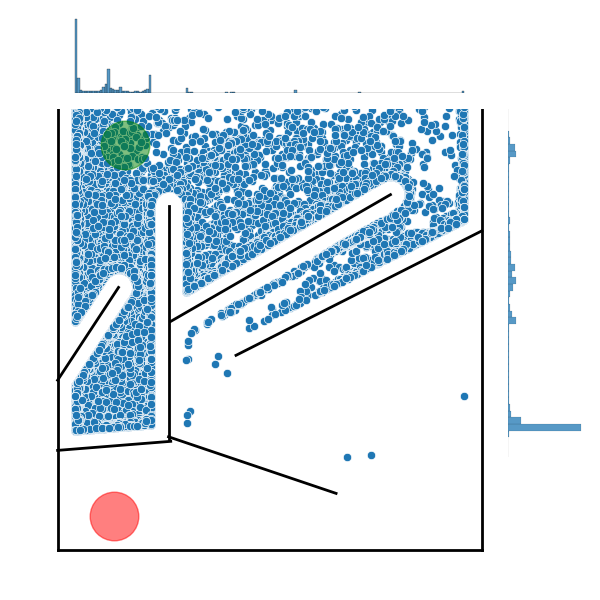
\includegraphics[scale=0.4]{resources/mazes/pure_fitness_open_all_runs.png}
            \caption{Fitness.}
        \end{subfigure}
        \begin{subfigure}[b]{0.5\textwidth}
            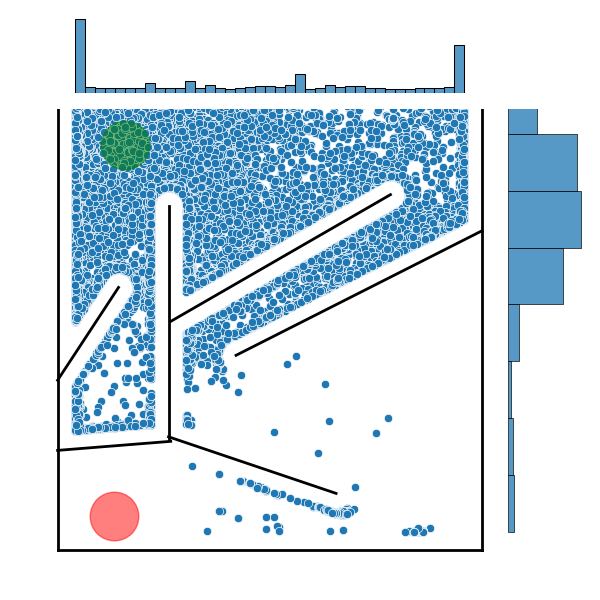
\includegraphics[scale=0.4]{resources/mazes/pure_novelty_open_all_runs.png}
            \caption{Novelty.}
        \end{subfigure}
        \begin{subfigure}[b]{0.5\textwidth}
            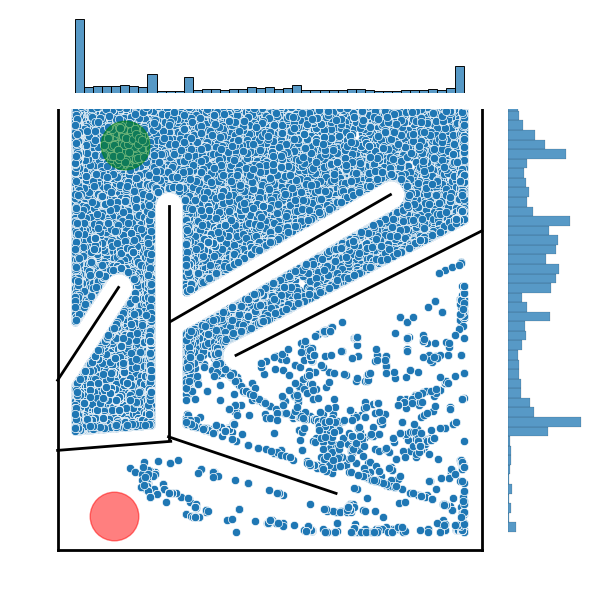
\includegraphics[scale=0.4]{resources/mazes/fitness_novelty_open_all_runs.png}
            \caption{LS-50.}
        \end{subfigure}
        \begin{subfigure}[b]{0.5\textwidth}
            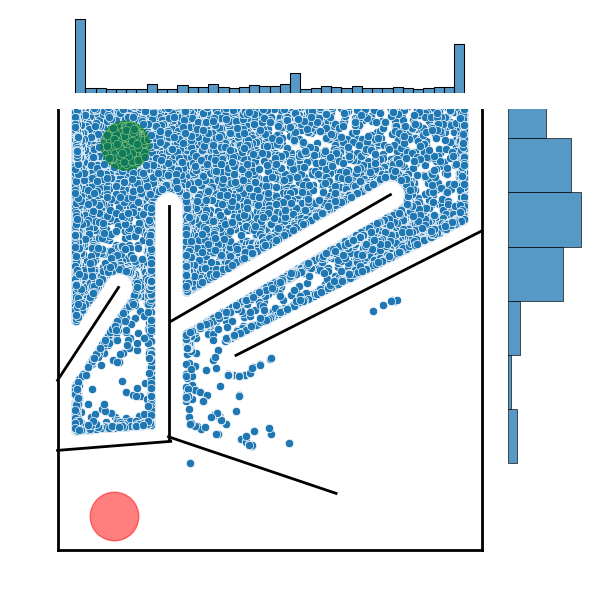
\includegraphics[scale=0.4]{resources/mazes/dynamic_open_all_runs.png}
            \caption{Dynamic linearisation.}
        \end{subfigure}
        \begin{subfigure}[b]{0.5\textwidth}
            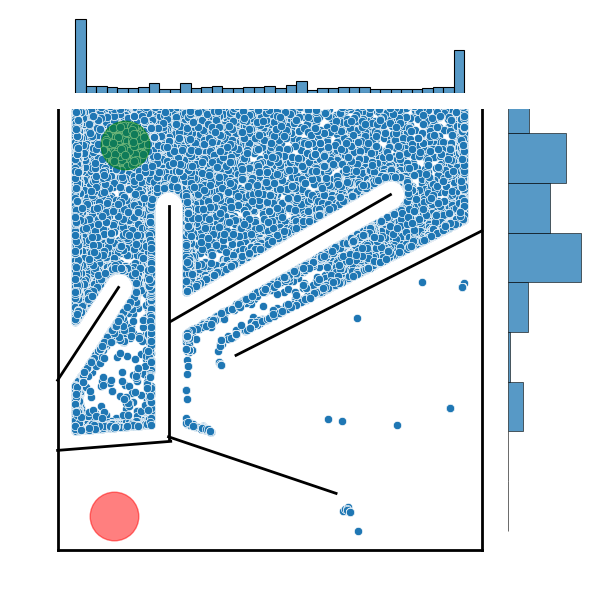
\includegraphics[scale=0.4]{resources/mazes/novelty_injection_open_all_runs.png}
            \caption{Novelty injection.}
        \end{subfigure}
    \end{mdframed}
    \caption{The distribution of all end-positions for each variant in the open maze.
             The top part of the maze is not shown.}
    \label{distribution_open}
\end{figure}


\section{Conclusion}
\label{sec:conclusion}
Neither of the proposed combinations of fitness and novelty search was significantly better
than LS-50 on any of the mazes. The robustness of the proposed combinations was not studied, so
it might be the case that the combinations perform better with other values. It might also be the
case that it is more appropriate to adjust $\rho$ based on another measure of the progress of
the search.



\clearpage
\hypersetup{breaklinks=true}
%\bibliographystyle{plainnat}
\bibliographystyle{unsrt}
\bibliography{bibliography/references.bib}

\end{document}
